\documentclass[10pt]{article}

% add links to document
\PassOptionsToPackage{hyphens}{url}\usepackage[hidelinks]{hyperref}

% add some packages
\usepackage{xcolor}
\usepackage[english]{babel}
\usepackage{nameref}
\usepackage{footnote}
\usepackage{refcount}
\usepackage{makecell}
\usepackage[a4paper, total={6in, 10in}]{geometry}
\usepackage{titlesec}
\usepackage{graphicx,import}
\usepackage{setspace}
\usepackage{url}
\usepackage{amsmath,amsfonts,amssymb}
%\usepackage{indentfirst}
\usepackage{float}
\usepackage{pgf}
\usepackage{pdfpages}
\usepackage{svg}
\usepackage{pstricks}
\usepackage{color,soul}
\usepackage{pst-plot}
\usepackage{import}
\usepackage{xifthen}
\usepackage{pdfpages}
\usepackage{transparent}
\usepackage[utf8]{inputenc}
\usepackage{csquotes}
\usepackage[style=verbose-ibid,backend=bibtex]{biblatex}
\usepackage{multirow}
\usepackage{caption}
\usepackage{colortbl}\usepackage{float}

\restylefloat{table}

% italic blockquotes
\renewcommand{\mkbegdispquote}[2]{\itshape}
\renewcommand{\mkbegdispquote}[2]{\openautoquote}
\renewcommand{\mkenddispquote}[2]{\closeautoquote#1#2}

% literature reference
\bibliography{references}

% document settings
\author{Björn Hempel <bjoern@hempel.li>}

% add nice formated tables
\makesavenoteenv{tabular}
\makesavenoteenv{table}

% add automatic numbering
\setcounter{secnumdepth}{5}
\setcounter{tocdepth}{4}
\setlength\bibitemsep{1.5\itemsep}

% some formating settings
\setlength{\parindent}{20pt}
\setlength{\parskip}{5pt}
\titleformat{\paragraph}
{\normalfont\normalsize\bfseries}{\theparagraph}{1em}{}
\titlespacing*{\paragraph}
{0pt}{3.25ex plus 1ex minus .2ex}{1.5ex plus .2ex}

% Footmarks always at the end of the page
\usepackage[bottom]{footmisc}

% allow some special characters
\DeclareUnicodeCharacter{2212}{-}

% pgf figures with images (add function \inputpgf)
\newcommand\inputpgf[2]{{
\let\pgfimageWithoutPath\pgfimage
\renewcommand{\pgfimage}[2][]{\pgfimageWithoutPath[##1]{#1/##2}}
\input{#1/#2}
}}

% import function of tex files
\newcommand{\includetex}[1]{
    \def\svgwidth{\columnwidth}
    \import{images/other/}{#1.pdf_tex}
}

% add language switcher functions \de and \en
\newif\ifen
\newif\ifde
\newcommand{\en}[1]{\ifen#1\fi}
\newcommand{\de}[1]{\ifde#1\fi}

% language switcher
%\detrue
\entrue



% -------------------- %
% Start document %
% -------------------- %
\begin{document}



	% -------------------- %
	% Flyleaf %
	% -------------------- %
	\thispagestyle{empty}


\includegraphics[width=0.4\textwidth]{images/tu_chemnitz}\\[2\baselineskip]

\begin{center}
\Large{TU Chemnitz}
\end{center}


\begin{center}
\Large{Faculty of Natural Sciences}\\
\Large{Institute of Physics}\\[4\baselineskip]
\end{center}

\begin{center}
\textbf{\LARGE{Bachelor Thesis}}\\[2\baselineskip]
\textbf{{In the course of degree in computational science (B.Sc.)}}
\end{center}

\begin{center}
\textbf{{To obtain the academic degree Bachelor of Science}}
\end{center}

\vspace*{\fill}
\begin{flushleft}
\begin{tabular}{llll}
\textbf{Topic:} & & Investigation of strategies for image classification \\
& & on small training data sets & \\
& & \\
\textbf{Author:} & & Björn Hempel \textless{bjoern@hempel.li}\textgreater & \\
& & Matriculation number 025038 & \\
& & \\
\textbf{Version from:} & & \today &\\
& & \\
\textbf{First assessor:} & & Prof. Dr. Angela Thränhardt &\\
\textbf{Second assessor:} & & Dr. David Urbansky &\\
\end{tabular}
\end{flushleft}




	\pagebreak



	% -------------------- %
	% Empty page %
	% -------------------- %
    \newpage\null\thispagestyle{empty}\newpage



	% -------------------- %
	% Abstract %
	% -------------------- %
	\section*{Abstract}
		\de{Neuronale Netze sind außerordentlich gut darin Muster in Daten zu finden. Hierzu müssen diese Netze vorher mit bekannten Datensätzen trainiert und entsprechend angepasst werden. Datensätze sind meist sehr teuer in der Beschaffung und sollten deshalb mit Bedacht und guter Qualität eingesetzt werden. Das Training des Netzes findet unter von vielen verschiedenen Parametern und Verfahrenstechniken statt. Dabei ist darauf zu achten das bestmögliche Modell mit seinen bestmöglichen Parametern zu verwenden. In dieser Arbeit werden gängige moderne Methoden der Bildklassifikation vorgestellt und miteinander verglichen. Das Hauptziel der Arbeit ist es, optimale Parameter und Techniken für die Klassifikation zu finden, die es auch ermöglichen, mit wenig Trainingsdaten ein optimales Modell zu erstellen.}
		\en{Neural networks are extraordinarily good at finding patterns in data. For this purpose, these networks must be trained with known data sets and adapted accordingly. Data sets are usually very expensive to obtain and should therefore be used with care and good quality. The training of the network takes place under many different parameters and process techniques. Care must be taken to use the best possible model with its best possible parameters. In this thesis, common modern methods of image classification will be presented and compared with each other. The main goal of the work is to find optimal parameters and techniques for the classification, which also allow to create an optimal model with little training data.}
	\pagebreak



	% -------------------- %
	% Table of contents %
	% -------------------- %
	\tableofcontents
	\pagebreak


	% -------------------- %
	% Introduction %
	% -------------------- %
	\section{Introduction}
		\de{In dieser Arbeit werden verschiedene Techniken der Bildklassifizierung verglichen. Variable Parameter beim Training werden einen entscheidenden Einfluss auf die Genauigkeit des Modells haben und werden hier im Detail verglichen. Nicht immer ist nur die Genauigkeit ein ausschlaggebender Faktor. Auch die benötigte Rechenzeit, welche notwendig ist das Modell zu bestimmen, soll nicht außer Acht gelassen werden und mit in die Auswertung einbezogen werden. Ich gehe davon aus, dass eine kleine Lernrate verbunden mit vielen Lern-Epochen und entsprechend mehr benötigter Rechenzeit bessere Ergebnisse erzielen werden, als wenige Lernepochen verbunden mit einer hohe Lernrate (langsame Anpassung vs. schnelle Anpassung). Auch gehe ich davon aus, dass eine hohe Qualität und eine größere Menge an Daten das Ergebnis entschieden positiv beeinflussen werden. Neue und komplexere Convolutional Neuronale Netzwerke stufe ich erfolgreicher in der Modellgenauigkeit ein als schön etwas ältere und kleinere Modelle.}
		\en{In this thesis different techniques of image classification are compared. Variable parameters during training will have a decisive influence on the accuracy of the model and are compared here in detail. Not always only the accuracy is a decisive factor. Also the required computing time, which is necessary to determine the model, should not be disregarded and should be included in the evaluation. I assume that a small learning rate combined with many learning epochs and correspondingly more computing time required will achieve better results than a few learning epochs combined with a high learning rate (slow adaptation vs. fast adaptation). I also assume that a high quality and a larger amount of data will have a decidedly positive influence on the result. New and more complex convolutional neural networks are more successful in model accuracy than older and smaller models.}


	% -------------------- %
	% Background %
	% -------------------- %
	\section{Background}

		% -------------------- %
		% Image Classification %
		% -------------------- %
		\subsection{Image Classification}
			\de{Klassifizierungen sind ein Prozess der Identifizierung, zu welcher Klasse ein unbeobachtetes Objekt gehört. Hierbei können eine Reihe von vordefinierten Klassen vorgegeben und anhand deren Eigenschaften versucht werden unbekannte und bisher unbeobachtete Objekt einzuordnen. Bei der Bildklassifizierung wird analog vorgegangen. Bei den zuvor genannten Objekten handelt es sich nun schlichtweg um Bilder.}
			\en{Classifications are a process of identifying to which class an unobserved object belongs. A number of predefined classes can be specified and, based on their properties, an attempt can be made to classify unknown and previously unobserved objects. The procedure for image classification is similar. The previously mentioned objects are now simply images.}

			\begin{figure}[H]
				\centering
				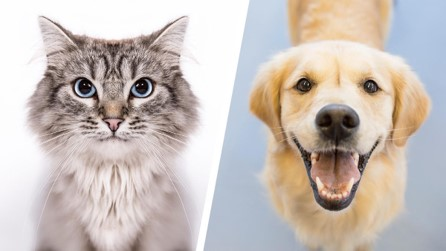
\includegraphics[width=0.4\textwidth]{images/cat_dog}
				\caption[Is it a dog or a cat?]{Is it a dog or a cat?\footnotemark}
				\label{fig:cat_or_dog}
			\end{figure}
			\footnotetext{Source: \url{https://towardsdatascience.com/image-classifier-cats-vs-dogs-with-convolutional-neural-networks-cnns-and-google-colabs-4e9af21ae7a8}}

			\de{Lange Zeit galt die automatische Erkennung von Objekten, Personen und Szenen in Bildern durch Computer als unmöglich. Die Komplexität schien zu groß, als dass man sie einem Algorithmus programmatisch beibringen könnte. Bis noch vor einigen Jahrzehnten hat man so versucht Bildklassifikation durch manuell entwickelte Algorithmen zu erreichen. Die automatisierte Klassifikation anhand von vorgegebenen und vorklassifizierten Bildern und dem automatisierten Erstellen von Modellen war ein neuer Schritt in eine neue Vorgehensweise. Die dabei entwickelten neuronale Netze spielten eine gewaltige Rolle und änderten dramatisch die Art der Herangehensweise! Mittlerweile ist die Bilderkennung ein weit verbreitetes Anwendungsgebiet des maschinellen Lernens. Häufig werden für Bilder sogenannte "Convolutional Neural Networks\footnote{Convolutional neural network, Wikipedia contributors, January 31, 2020, \url{https://en.wikipedia.org/wiki/Convolutional_neural_network}}" or "ConvNets" are often used for images.}
			\en{For a long time, the automatic recognition of objects, people and scenes in images by computers was considered impossible. The complexity seemed too great to be programmatically taught to an algorithm. Until a few decades ago, attempts were made to achieve image classification by manually developed algorithms. Automated classification based on given and pre-classified images and the automated creation of models was a new step into a new approach. The neural networks developed in this process played a huge role and dramatically changed the way of approach! In the meantime, image recognition has become a widespread application area of machine learning. So-called "Convolutional Neural Networks\footnote{Convolutional neural network, Wikipedia contributors, January 31, 2020, \url{https://en.wikipedia.org/wiki/Convolutional_neural_network}}" or "ConvNets" are often used for images.}

			\de{Der Bildklassifizierungsalgorithmus nimmt ein Bild als Eingabe und klassifiziert es in eine der Ausgabekategorien. Deep Learning hat den Bereich der Bildklassifizierung revolutioniert und großartige Ergebnisse erzielt. Verschiedene Deep Learning Netzwerke, wie ResNet, DenseNet, Inception, etc. wurden als hochpräzise Netzwerke für die Bildklassifikation entwickelt. Gleichzeitig wurden Bilddatensätze angelegt, um getaggte Bilddaten zu erfassen. Diese werden jetzt vorrangig dazu verwendet um bestehende Netzwerke zu trainieren und alljährliche Challenges zu veranstalten, welche sich mit den bisher bekannten und schon entwickelten Modellgenauigkeiten messen. ImageNet ist ein solch großer Datensatz mit mehr als 11 Millionen Bildern und über 11.000 Kategorien. Wenn ein Netzwerk einmal mit ImageNet-Daten trainiert wurde, kann es durch einfache Neuanpassung oder Optimierung mit anderen Datensätzen verallgemeinert werden. Bei diesem Transfer-Lernansatz wird ein Netzwerk mit Gewichten initialisiert, welche aus einem zuvor trainierten Netzwerk stammen. Dieses zuvor initialisierte Netzwerk wird nun für eine neue Bildklassifikationsaufgabe lediglich entsprechend angepasst.}
			\en{The image classification algorithm takes an image as input and classifies it into one of the output categories. Deep Learning has revolutionized the field of image classification and has achieved great results. Various Deep Learning networks, such as ResNet, DenseNet, Inception, etc. have been developed as high-precision networks for image classification. At the same time, image data sets were created to capture tagged image data. These are now primarily used to train existing networks and to organize annual challenges that compete with the model accuracies already known and developed. ImageNet is such a large data set with more than 11 million images and over 11,000 categories. Once a network has been trained with ImageNet data, it can be generalized with other data sets by simple re-compilation or optimization. In this transfer learning approach, a network is initialized with weights that come from a previously trained network. This previously initialized network is now simply adapted for a new image classification task.}

			\de{Die hier zugrunde liegende Arbeit beschäftigt sich hauptsächlich mit überwachtem Lernen, bei dem ein mathematisches Modell aufgrund bestehender bekannter Datensätze trainiert wird. Das Ziel des trainierten Modells ist es dabei auch für unbekannte Bilder bestmögliche Vorhersagen zu treffen. Diese bekannten Datensätze werden meist händisch erstellt (Ontologe), automatisiert aufgrund bekannter Tatsachen bestimmt oder auch in einem halbautomatischen Prozess ermittelt.}
			\en{The underlying work here is mainly concerned with supervised learning, in which a mathematical model is trained based on existing known data sets. The goal of the trained model is to make best possible predictions even for unknown images. These known data sets are usually created manually (ontologist), automatically determined based on known facts or determined in a semi-automatic process.}
			
		% -------------------- %
		% Deductive approach %
		% -------------------- %
		\subsubsection{Deductive approach}
		\label{sec:section_deductive_approach}
			\de{Seit den späten 1960er Jahren hat man versucht, Bilder mit selbstgeschriebenen Algorithmen zu klassifizieren. Dieser Teil der Computer Vision beschäftigt sich mit Techniken wie Bildentstehung, Bildbearbeitung und Bildsegmentierung. Im Bereich der Bildverarbeitung reihen sich bekannte Verfahren wie Kantenerkennungen, Merkmalsdetektoren, Randverknüpfungen, Kontrastverbesserungen, etc.\footnote{Szeliski, R.: Computer Vision: Algorithms and Applications,  Springer Science Business Media, 10 (2010)\label{springer_10}} Allen Techniken gemein ist die Verwendung des deduktiven Ansatzes. Beim deduktiven Ansatz erstellt man Regeln (Merkmalsdetektoren), welche das gewünschte Ergebnis vorhersagen sollen. Diese Regeln werden vorgegeben und beschrieben und erlauben damit später eine Klassifizierung von unbekannten Objekten. Da das Modell und sein Algorithmus hinreichend bekannt ist, wird dieses Verfahren White-Box-Verfahren genannt.}
			\en{Since the late 1960s, attempts have been made to classify images with self-written algorithms. This part of Computer Vision deals with techniques such as image creation, image processing and image segmentation. In the field of image processing, well-known techniques such as edge detection, feature detectors, edge linking, contrast enhancement, etc. are used\footnote{Szeliski, R.: Computer Vision: Algorithms and Applications,  Springer Science Business Media, 10 (2010)\label{springer_10}}. Common to all techniques is the use of the deductive approach. With the deductive approach, one creates rules (feature detectors) which are supposed to predict the desired result. These rules are given and described and thus allow later classification of unknown objects. Since the model and its algorithm are sufficiently well known, this procedure is called white-box procedure.}

			\begin{figure}[H]
				\begin{center}
					\scalebox{1.0}{\includetex{deductive_approach}}
				\end{center}
				\caption{Deductive approach}
				\label{fig:overview_deductive_approach}
			\end{figure}

			\de{}

		% -------------------- %
		% Inductive approach %
		% -------------------- %
		\subsubsection{Inductive approach}
		\label{sec:section_inductive_approach}
			\de{Der induktive Ansatz hingegen verfolgt einen anderen Ansatz Bilder zu klassifizieren. Das Ziel ist nicht die Vorgabe einer Regel, sondern das Vorgehen aus schon bekannten einzelnen Objekten eine Regel (Modell) automatisiert zu erlernen. Ein Modell meist eine komplexe Funktion und eine mathematische Abbildung eines Raumes (VC Dimension\footnote{Vapnik–Chervonenkis dimension, Wikipedia contributors, January 31, 2020, \url{https://en.wikipedia.org/wiki/Vapnik\%E2\%80\%93Chervonenkis_dimension}}), in welcher einzelne Objekte mit ihren Eigenschaften abgebildet und getrennt werden können. Das Modell wird Stück für Stück den bekannten Objekten so angepasst, dass der Eingabewert dem Ausgabewert entspricht bzw. weitgehend entspricht (Backpropagation). Das Ziel ist es mit diesem Modell eine Funktion zu erstellen, welche in der Lage ist auch unbekannte Objekte bestmöglichst zu klassifizieren. Da der Raum dieses Modell meist fern der Vorstellungskraft und der Erklärungsmöglichkeit liegt, wird dieses Verfahren auch Black-Box-Verfahren genannt. Der hier beschriebene Vorgang wird meist bei jeder Art von \hyperref[sec:section_supervised_classification]{überwachtem Lernen} angewendet und ist ein Teil des \hyperref[sec:section_machine_learning]{maschinellem Lernens}.}
			\en{The inductive approach, on the other hand, takes a different approach to classifying images. The goal is not to specify a rule, but to learn a rule (model) automatically from already known individual objects. A model is usually a complex function and a mathematical representation of a space (VC dimension\footnote{Vapnik–Chervonenkis dimension, Wikipedia contributors, January 31, 2020, \url{https://en.wikipedia.org/wiki/Vapnik\%E2\%80\%93Chervonenkis_dimension}}), in which individual objects with their properties can be mapped and separated. The model is adapted piece by piece to the known objects in such a way that the input value corresponds to the output value or corresponds to a large extent (backpropagation). The goal is to create a function with this model, which is able to classify unknown objects in the best possible way. Because the space of this model is mostly far away from the imagination and the possibility of explanation, this procedure is also called black box procedure. The procedure described here is mostly used for any kind of \hyperref[sec:section_supervised_classification]{supervised learning} and is a part of \hyperref[sec:section_machine_learning]{machine learning}.}

			\begin{figure}[H]
				\begin{center}
					\scalebox{1.0}{\includetex{inductive_approach}}
				\end{center}
				\caption{Inductive approach}
				\label{fig:overview_inductive_approach}
			\end{figure}

		% -------------------- %
		% Balanced training data set %
		% -------------------- %
		\subsubsection{Balanced training data set}
		\label{sec:section_balanced_training_data_set}
			\de{Neuronale Netze haben in den letzten Jahren enorme Fortschritte im Bereich der Mustererkennung gemacht. Dabei ist ein entscheidender Faktor, dass die Daten zum Lernen eine hohe Qualität und eine einfache Verarbeitung für das Netzwerk aufweisen müssen. Falsch klassifizierte oder irrelevante Daten könnten dazu führen, dass das Netzwerk was Falsches lernt. Das gilt auch für eine nicht vorhandene bzw. nicht geeignete Vorverarbeitung.}
			\en{Neural networks have made enormous progress in the field of pattern recognition in recent years. A decisive factor is that the data for learning must be of high quality and easy for the network to process. Wrongly classified or irrelevant data could cause the network to learn something wrong. This also applies to non-existent or unsuitable pre-processing\autocite{osinga2019data}.}

			\de{Mit dem Beginn eines Klassifizierungsprojektes steht die Frage was genau man klassifizieren möchte und wie umfangreich die Klassifzierung ausfallen soll. Angenommen man möchte verschiedene Klassen von Essen identifizieren, so könnten das Klassen wie Pizza, Burger, Donuts und Lasagne sein (etc.). Zu diesen Klassen benötigt man nun eine große Anzahl an Bildern. Diese Daten sollten im Idealfall die Realität möglichst gut widerspiegeln. Eine große Variation ist von Vorteil (ausbalancierter Datenset): verschiedene Blickwinkel, Größe, Position, Farbhelligkeiten, Variationen, Anzahl, etc. Bilder von z.B. nur einer Farbhelligkeit oder nur einem Blickwinkel sollten vermieden werden. Sind die Daten nicht ausbalanciert, so müssen diese entsprechend korrigiert werden: z.B. durch Hinzufügen weiterer Daten, Bildverarbeitung oder durch Entfernen von Daten, welche für eine Unausgewogenheit sorgen. Weiterhin sollten die ausgewählten Klassen untereinander klar optisch trennbar sein. Sind sich zwei Klassen optisch sehr ähnlich und selbst durch einen Menschen nicht wirklich unterscheidbar, sollte darüber nachgedacht werden diese zusammenzufassen (z.B. "burger" und "veggie burger"):}
			\en{With the beginning of a classification project the question is what exactly you want to classify and how extensive the classification should be. Assuming you want to identify different classes of food, this could be classes like pizza, burgers, donuts and lasagna (etc.). For these classes you now need a large number of images. Ideally, this data should reflect reality as well as possible. A large variation is advantageous (balanced data set): different viewing angles, size, position, colour brightness, variations, number, etc. Images of e.g. only one colour brightness or only one viewing angle should be avoided. If the data are not balanced, they must be corrected accordingly: e.g. by adding further data, image processing or by removing data that causes an imbalance. Furthermore, the selected classes should be clearly optically separable from each other. If two classes are visually very similar and not really distinguishable even by a human, consideration should be given to combining them (e.g. "burger" and "veggie burger"):}

			\begin{figure}[H]
				\centering
				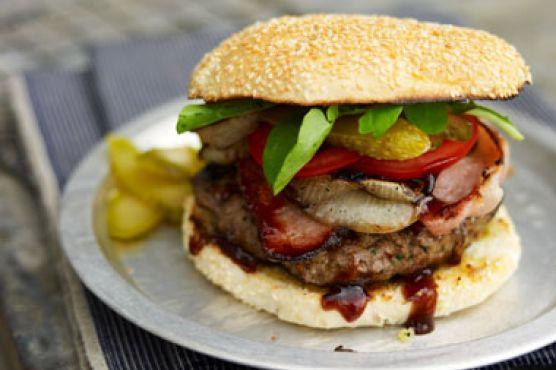
\includegraphics[width=0.19\textwidth]{images/data/burger/burger28.jpg}
				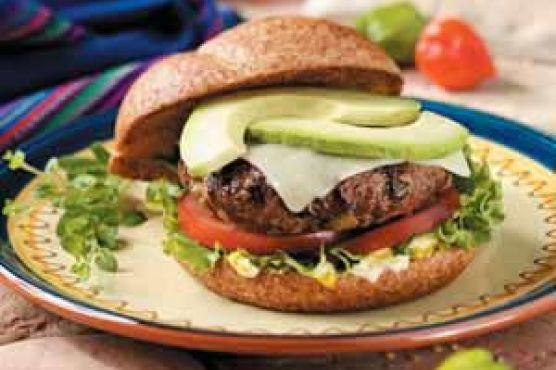
\includegraphics[width=0.19\textwidth]{images/data/burger/burger77.jpg}
				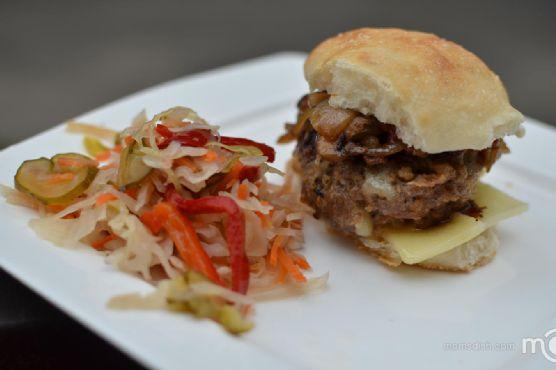
\includegraphics[width=0.19\textwidth]{images/data/burger/burger89.jpg}
				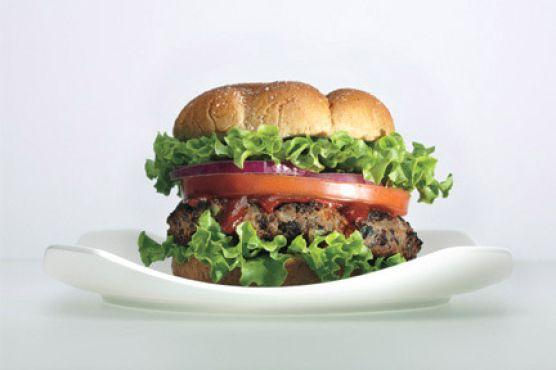
\includegraphics[width=0.19\textwidth]{images/data/burger/burger162.jpg}
				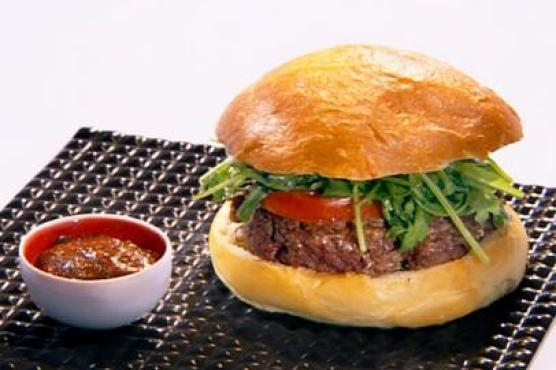
\includegraphics[width=0.19\textwidth]{images/data/burger/burger449.jpeg}
				\caption[Example pictures of a burger class]{Example pictures of a burger class}
				\label{fig:class_burger}
			\end{figure}

			\begin{figure}[H]
				\centering
				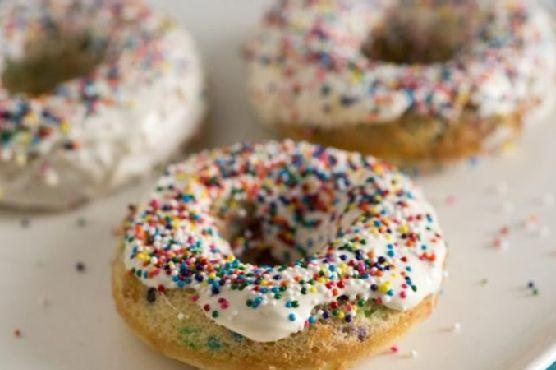
\includegraphics[width=0.19\textwidth]{images/data/donut/donut116.jpg}
				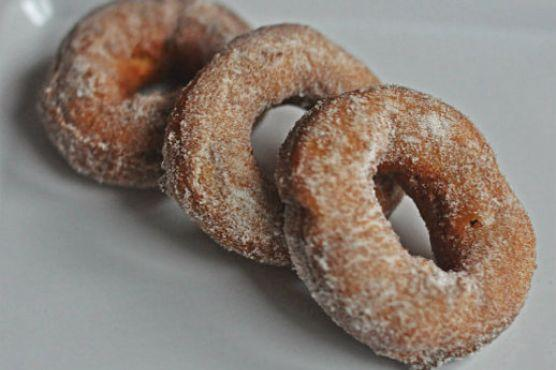
\includegraphics[width=0.19\textwidth]{images/data/donut/donut155.jpg}
				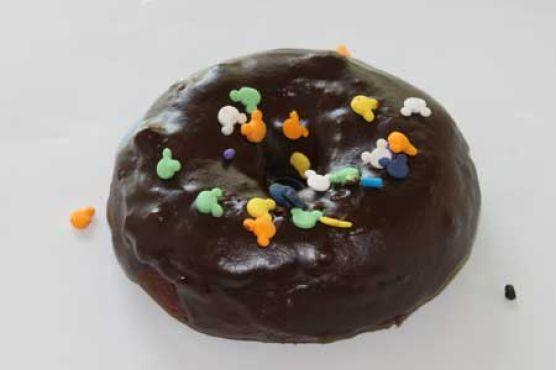
\includegraphics[width=0.19\textwidth]{images/data/donut/donut176.jpg}
				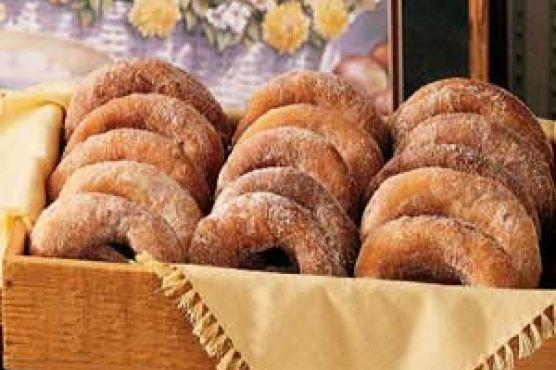
\includegraphics[width=0.19\textwidth]{images/data/donut/donut205.jpg}
				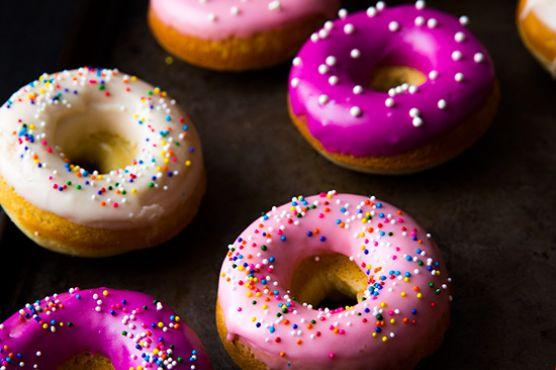
\includegraphics[width=0.19\textwidth]{images/data/donut/donut440.jpg}
				\caption[Example pictures of a donut class]{Example pictures of a donut class}
				\label{fig:class_donut}
			\end{figure}

			\begin{figure}[H]
				\centering
				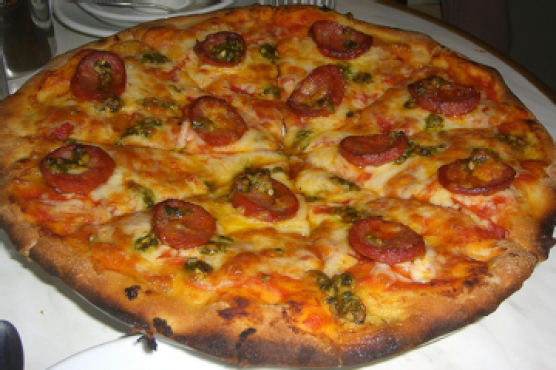
\includegraphics[width=0.19\textwidth]{images/data/pizza/pizza73.png}
				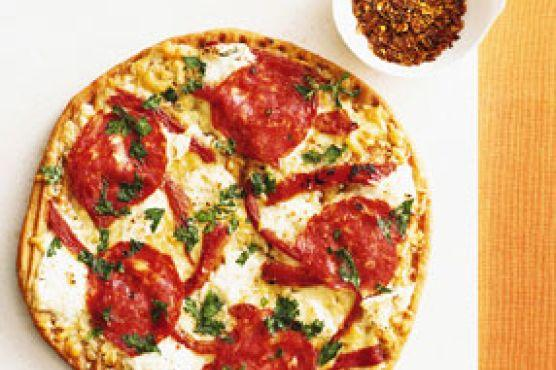
\includegraphics[width=0.19\textwidth]{images/data/pizza/pizza76.jpg}
				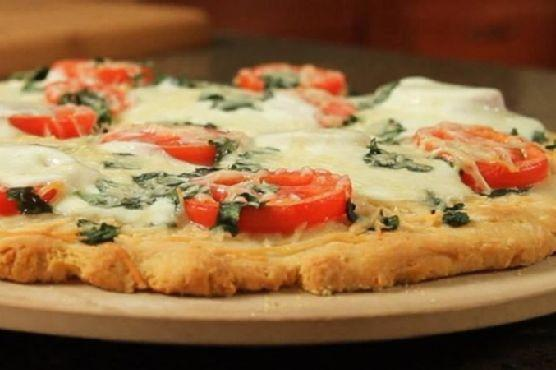
\includegraphics[width=0.19\textwidth]{images/data/pizza/pizza92.jpg}
				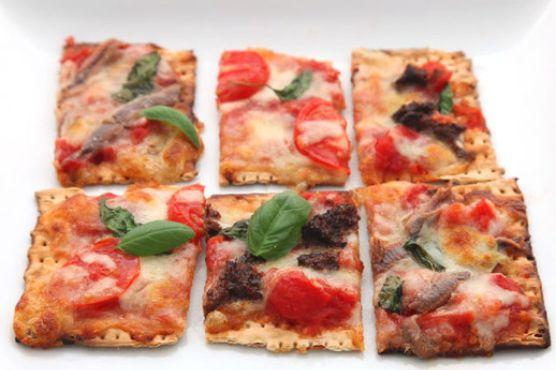
\includegraphics[width=0.19\textwidth]{images/data/pizza/pizza108.jpg}
				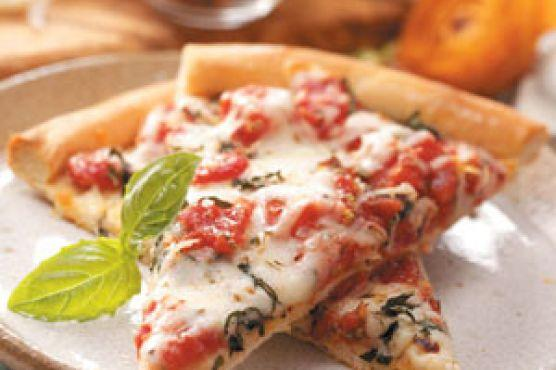
\includegraphics[width=0.19\textwidth]{images/data/pizza/pizza239.jpg}
				\caption[Example pictures of a pizza class]{Example pictures of a pizza class}
				\label{fig:class_pizza}
			\end{figure}

			\de{An Daten zu gelangen ist oftmals nicht so einfach. Jede Datenquelle hat ihre eigenen Besonderheiten. Eine Möglichkeit an Daten zu gelangen wäre ein automatische Crawling von Bilddatenbanken, Suchmaschinen oder Rezensionen, in welchen Bilder vorkommen. Ein gewisses Maß an Kreativität ist von Vorteil:}
			\en{Accessing data is often not that easy. Every data source has its own special features. One way to access data would be an automatic crawling of image databases, search engines or reviews in which images appear. A certain amount of creativity is advantageous:}

			\begin{itemize}
				\item Google
				\item Bing
				\item Flickr
				\item TripAdvisor
				\item etc.
			\end{itemize}
			
			\de{Die wahrscheinlich teuerste Variante an Daten zu gelangen ist die händische Suche und Klassifizierung durch z.B. einen Ontologen. Dieser beurteilt und sucht verschiedenen Bilder und ordnet diese händisch in die entsprechenden Klassen ein. Auch eine kombinierte Variante ist möglich und wahrscheinlich zu bevorzugen: Automatisches Crawling und händisches aussortieren falscher, ungünstiger oder irrelevanter Bilder.}
			\en{Probably the most expensive way to obtain data is to search and classify them manually, e.g. by an ontologist. The ontologist evaluates and searches for different images and manually classifies them in the appropriate classes. A combined variant is also possible and probably preferable: automatic crawling and manual sorting out of incorrect, unfavorable or irrelevant images.}

		% -------------------- %
		% Training, test and evaluation data set %
		% -------------------- %
		\subsubsection{Training, test and evaluation data set}
		\label{sec:section_training_test_and_evaluation}
			\de{Vor dem Beginn mit dem Training von ausbalancierten Bildern müssen diese in einen Trainings-, einen Test- und eventuell in einen Validierungsdatensatz aufgeteilt werden. Dies ist notwendig, da neuronale Netze zu einem Teil nicht verallgemeinern, sondern auswendig lernen werden (overfitting\footnote{``Overfitting'', Wikipedia contributors, January 31, 2020, \url{https://en.wikipedia.org/wiki/Overfitting}}). Die Idee ist es mit einem Trainingsdatensatz zu trainieren, während mit dem Validierungsdatensatz die Allgemeingültigkeit des Netzes und seiner Parameter überwacht wird. Anhand der Ergebnisse werden zur Laufzeit Anpassungen vorgenommen. Da die Anpassung der Parameter anhand der Testdaten vorgenommen wird, gibt es noch einen unabhängigen Testdatensatz, welcher eine erneute Überprüfung des Modells auf bisher unbeteiligte Daten vornimmt. Dieser stellt sicher, dass nicht versehentlich Hyperparameter nur speziell für den Validierungsdatensatz optimiert werden\autocite{osinga2019data}. Die Verwendung des Testdatensatz ist optional und simuliert das Modell unter realen Bedingungen. Ist die Anzahl der Daten begrenzt und kann dieser Datensatz z.B. auch dem Trainingsdatensatz hinzugefügt werden. In dieser Arbeit wird auf den Testdatensatz verzichtet und sämtliche Auswertungen beziehen sich auf den Validierungsdatensatz.}
			\en{Before starting the training of balanced images, they must be divided into a training, a test and possibly a validation data set. This is necessary because neural networks will not generalize to some extent, but will learn by heart (overfitting\footnote{``Overfitting'', Wikipedia contributors, January 31, 2020, \url{https://en.wikipedia.org/wiki/Overfitting}}). The idea is to train with a training data set, while the validation data set is used to monitor the general validity of the network and its parameters. Based on the results, adjustments are made at runtime. Since the adjustment of the parameters is carried out using the test data, there is also an independent test data set, which carries out a renewed check of the model for previously uninvolved data. This ensures that hyperparameters are not inadvertently optimized for the validation data set only\autocite{osinga2019data}. The use of the test data set is optional and simulates the model under real conditions. If the number of data is limited, this data record can also be added to the training data record, for example. In this thesis, the test data set is not used and all evaluations refer to the validation data set.}

			\de{Eine optimale Aufteilung des Trainings- und Validierungsdatensatzes ist abhängig von dem vorliegenden Klassifizierungsproblem und die Anzahl der Daten, welche zur Verfügung stehen. In dieser Arbeit wird ein Verhältnis aus 80 Prozent Trainingsdaten und 20 Prozent Validierungsdaten verwendet, sofern nicht anders angegeben.}
			\en{An optimal division of the training and validation data set depends on the existing classification problem and the amount of data available. In this paper a ratio of 80 percent training data and 20 percent validation data is used, unless otherwise stated.}

			\de{\hl{Hier muss die Frage noch geklärt werden warum 80 Prozent Trainingsdaten und 20 Prozent Validierungsdaten verwendet werden. Gibt es ein Paper bzw. eine Studie dazu? Oder ist noch ein Test erforderlich?}}
			\en{\hl{The question of why 80 percent training data and 20 percent validation data are used remains to be clarified. Is there a paper or a study on this? Or is another test required?}}			

		% -------------------- %
		% Methods of machine learning %
		% -------------------- %
		\subsubsection{Methods of machine learning}
		\label{sec:section_methods_of_machine_learning}
			\de{Je nach Art und Vorgehensweise der Überwachung des Trainings lassen sich verschiedene Machine-Learning-System einordnen. Dabei wird unterschieden, welche Art von Daten uns vorliegen oder diese selbst bestimmt werden müssen.}
			\en{Different machine learning systems can be classified according to the type and procedure of monitoring the training. A distinction is made between the type of data we have or the data we need to determine ourselves.}

			% -------------------- %
			% Supervised learning %
			% -------------------- %
			\paragraph{Supervised learning}
			\label{sec:section_supervised_learning}
				\de{Das überwachte Lernen bezieht sich auf ein maschinelles Lernen mit bekannten Trainingsdatensätzen (siehe auch Kapitel ``induktiver Ansatz''\hyperref[sec:section_inductive_approach]). Der Lernprozess wiederrum bezieht sich auf die Fähigkeit einer künstlichen Intelligenz, Regelmäßigkeiten und Muster zu reproduzieren. Die Ergebnisse sind durch Naturgesetze oder Expertenwissen bekannt und werden für die Lehre des Systems verwendet, in dem ein Trainingsset erstellt wird, welcher die gewünschten Lösungen enthält. Man nennt dies auch gelabelte Daten. Der Lernalgorithmus versucht nun epochenweise eine Hypothese zu finden, die eine möglichst genaue Vorhersagen auf unbekannten Daten ermöglicht. Eine Hypothese ist in diesem Fall ein Bild, das jedem Eingabewert (das Bild selbst) den angenommenen Ausgabewert (die vorhergesagte Klasse) zuordnet. Diese Arbeit macht ausgiebigen Gebrauch von überwachtem Lernen.}
				\en{Supervised learning refers to machine learning with known training data sets (see also chapter ``inductive approach''\hyperref[sec:section_inductive_approach]). The learning process in turn refers to the ability of an artificial intelligence to reproduce regularities and patterns. The results are known by laws of nature or expert knowledge and are used to teach the system by creating a training set containing the desired solutions. This is also called labelled data. The learning algorithm now tries to find a hypothesis epoch by epoch, which allows the most accurate predictions on unknown data. A hypothesis in this case is an image that assigns the assumed output value (the predicted class) to each input value (the image itself). This work makes extensive use of supervised learning.}
	
				\de{Beim Überwachten Lernen wird einer Klassifizierungsfunktion (meist ein künstliches neuronales Netz) ein Eingangsvektor zugeführt. Der Eingangsvektor erzeugt mit Hilfe der Klassifizierungsfunktion einen Ausgabevektor, die dieses neuronale Netz in seinem aktuellen Zustand produziert\footnote{Das neuronale Netzwerk besteht aus vielen (meist Millionen) Parametern, welche während des Lernprozesses angepasst werden können, um den Fehler zu minimieren.}. Dieser Wert wird mit dem Wert verglichen, den es eigentlich ausgeben soll. Der Vergleich des Soll- und Istzustandes gibt Auskunft wie und in welcher Form Änderungen am Netzwerk vorgenommen werden müssen, um dem Istzustand weiter anzugleichen und den Fehler zu minimieren. Für künstliche neuronale Netzwerke ohne versteckter Schicht (einlagiges Perzeptron\footnote{``Perceptron'', Wikipedia contributors, February 2, 2020, \url{https://en.wikipedia.org/wiki/Perceptron}}) kann die Delta-Regel\footnote{``Least mean squares'' filter also known as ``delta rule'', Wikipedia contributors, February 2, 2020, \url{https://en.wikipedia.org/wiki/Least_mean_squares_filter}} für die Korrektur vorgenommen werden. Bei Netzwerken mit einer oder mehreren versteckten Schichten verwendet man Backpropagation\footnote{``Backpropagation'', Wikipedia contributors, February 2, 2020, \url{https://en.wikipedia.org/wiki/Backpropagation}} um den Fehler zu minimieren. Backpropagation ist eine Verallgemeinerung der Delta-Regel.}
				\en{In supervised learning, an input vector is fed to a classification function (usually an artificial neural network). The input vector generates an output vector using the classification function, which produces this neural network in its current state\footnote{The neural network consists of many (usually millions) parameters, which can be adjusted during the learning process to minimize the error.}. This value is compared with the value that it should actually output. The comparison of the nominal and actual state provides information on how and in what form changes must be made to the network in order to further approximate the actual state and minimize the error. For artificial neural networks without a hidden layer (single-layer perceptron\footnote{``Perceptron'', Wikipedia contributors, February 2, 2020, \url{https://en.wikipedia.org/wiki/Perceptron}}), the delta rule\footnote{``Least mean squares'' filter also known as ``delta rule'', Wikipedia contributors, February 2, 2020, \url{https://en.wikipedia.org/wiki/Least_mean_squares_filter}} for correction can be applied. For networks with one or more hidden layers backpropagation\footnote{``Backpropagation'', Wikipedia contributors, February 2, 2020, \url{https://en.wikipedia.org/wiki/Backpropagation}} is used to minimize the error. Backpropagation is a generalization of the delta rule.}
				
				\de{Das neuronale Netzwerke ist nur ein Algorithmus aus der Kategorie der überwachten Lernalgorithmen. Der Vollständigkeit hier noch eine Liste von weiteren Verfahren:}
				\en{The neural network is only one algorithm from the category of supervised learning algorithms. For completeness here is a list of further algorithms:}
				
				\begin{itemize}
					\item k-nearest neighbors\footnote{``k-nearest neighbors algorithm'', Wikipedia contributors, February 2, 2020, \url{https://en.wikipedia.org/wiki/K-nearest_neighbors_algorithm}}
					\item Linear regression\footnote{``Linear regression'', Wikipedia contributors, February 2, 2020, \url{https://en.wikipedia.org/wiki/Linear_regression}}
					\item Logistic regression\footnote{``Logistic regression'', Wikipedia contributors, February 2, 2020, \url{https://en.wikipedia.org/wiki/Logistic_regression}}
					\item Support-vector machine\footnote{``Support-vector machine'', Wikipedia contributors, February 2, 2020, \url{https://en.wikipedia.org/wiki/Support-vector_machine}}
					\item Random forest\footnote{``Random forest'', Wikipedia contributors, February 2, 2020, \url{https://en.wikipedia.org/wiki/Random_forest}}
					\item etc.
				\end{itemize}
		
			% -------------------- %
			% Unsupervised learning %
			% -------------------- %
			\paragraph{Unsupervised learning}
			\label{sec:section_unsupervised_learning}
				\de{Beim unüberwachtem Lernen versucht man auch ohne gelabelte Daten an eine Kenntnis von Mustern zu erlangen. Angenommen man hätte mehrere Bilder von Burgern, Pizza und Donuts, welche sich unsortiert in einem Datenset befinden. Das unüberwachte Lernen versucht nun Ähnlichkeiten zu finden, um diese Bilder zu gruppieren. Im besten Fall erhält man am Ende drei unbenannte Gruppen \(A\), \(B\) und \(C\). Analysten werden sich diese Gruppen im Nachgang genauer anschauen und ein Fazit daraus ziehen, sofern dies möglich ist: Gruppe \(A\) sind Burger, Gruppe \(B\) sind Pizzen, etc.}
				\en{In unsupervised learning, one tries to gain knowledge of patterns even without labelled data. Suppose you have several pictures of burgers, pizza and donuts, which are unsorted in a data set. Unsupervised learning now tries to find similarities in order to cluster these images. In the best case you get three unnamed groups \(A\), \(B\) and \(C\) at the end. Analysts will take a closer look at these groups afterwards and draw a conclusion if possible: Group \(A\) is burgers, group \(B\) is pizzas, etc. }
				
				\de{\noindent Folgende unüberwachte Lernalgorithmen können zur Gruppierung verwendet werden:}
				\en{\noindent The following unsupervised learning algorithms can be used for clustering:}
				
				\begin{itemize}
					\item k-means\footnote{``k-means clustering'', Wikipedia contributors, February 2, 2020, \url{https://en.wikipedia.org/wiki/K-means_clustering}}
					\item Hierarchical clustering\footnote{``Hierarchical clustering'', Wikipedia contributors, February 2, 2020, \url{https://en.wikipedia.org/wiki/Hierarchical_clustering}}
					\item Expectation–maximization \footnote{``Expectation–maximization algorithm'', Wikipedia contributors, February 2, 2020, \url{Expectation–maximization algorithm}}
					\item etc.
				\end{itemize}
			
				\de{Eine Technik, die hierarchische Clusteranalyse, wird später verwendet um die Einführung von Hierarchien zu erleichtern. Für die allgemeine Analyse, den Finden von optimalen Parametern für das Lernen von Modellen, wird diese Art des Lernens in dieser Arbeit nicht verwendet.}
				\en{One technique, hierarchical clustering, is used later to facilitate the introduction of hierarchies. For the general analysis, the finding of optimal parameters for learning models, this kind of learning is not used in this thesis.}

			% -------------------- %
			% Reinforcement learning %
			% -------------------- %
			\paragraph{Reinforcement learning}
			\label{sec:section_reinforcement_learning}
				\de{Reinforcement learning\footnote{``Reinforcement learning'', Wikipedia contributors, January 31, 2020, \url{https://en.wikipedia.org/wiki/Reinforcement_learning}} ist eine Art des maschinellen Lernens, bei der ein Agent selbstständig die bestmögliche Strategie für die Erreichung eines Zieles erlernt. Für die Erreichung des Ziels sind Aktionen notwendig, welche zu bestimmten Zeitpunkten Belohnungen hervorbringen. Diese Belohnungen können auch negative sein (Bestrafung). Anhand dieser Belohnungen gilt es in Summe den bestmöglichen Belohnungswert zu erzielen. Bei der Klassifizierung von Bildern ist diese Art des Lernens nicht relevant, weshalb hier auch nicht weiter darauf eingegangen wird.}
				\en{Reinforcement learning\footnote{``Reinforcement learning'', Wikipedia contributors, January 31, 2020, \url{https://en.wikipedia.org/wiki/Reinforcement_learning}} is a type of machine learning in which an agent independently learns the best possible strategy for achieving a goal. To achieve the goal, actions are necessary which produce rewards at certain points in time. These rewards can also be negative (punishment). Based on these rewards, the aim is to achieve the best possible reward value. This type of learning is not relevant for the classification of images, which is why it will not be discussed further here.}



		% -------------------- %
		% Classification Metrics %
		% -------------------- %
		\subsubsection{Classification Metrics and confusion matrix}
			\de{Die Wahl der richtigen Metrik ist bei der Bewertung von Modellen des maschinellen Lernens von entscheidender Bedeutung. Metriken werden zur Überwachung und Messung der Leistung eines Modells während des Trainings und des Tests verwendet. Im nachfolgenden werden einige wichtige Metriken erklärt.}
			\en{Choosing the right metric is crucial in evaluating machine learning models. Metrics are used to monitor and measure the performance of a model during training and testing. Some important metrics are explained below.}

			% -------------------- %
			% Confusion Matrix %
			% -------------------- %
			\paragraph{Confusion Matrix}
			 	\de{Die Confusion Matrix ist eine spezielle quadratische Matrix auf dem Gebiet des maschinellen Lernens, das die Visualisierung der Leistung eines Vorhersage-Modells ermöglicht. Jede Zeile der Matrix repräsentiert die tatsächliche Klasse, während jede Spalte die Anzahl oder eine Zahlenangaben in Prozent der vorhergesagten Klasse angibt (oder umgekehrt)\footnote{``Confusion matrix'', Wikipedia contributors, February 5, 2020, \url{https://en.wikipedia.org/wiki/Confusion_matrix}}:}
			 	\en{The Confusion Matrix is a special quadratic matrix in the field of machine learning that allows the visualization of the performance of a predictive model. Each row of the matrix represents the actual class, while each column indicates the number or a numerical value as a percentage of the predicted class (or vice versa)\footnote{``Confusion matrix'', Wikipedia contributors, February 5, 2020, \url{https://en.wikipedia.org/wiki/Confusion_matrix}}:}

				\begin{table}[htb]
					\centering
					{\def\arraystretch{2}\tabcolsep=5pt
						\begin{tabular}{cc|c|c|c|c|}
							\cline{3-6}
							& & \multicolumn{4}{c|}{\textbf{predicted}} \\ \cline{3-6} 
							& & \boldmath\(class_1\) & \boldmath\(class_2\) & \textbf{\ldots} & \boldmath\(class_n\) \\ \hline
							\multicolumn{1}{|l|}{\multirow{4}{*}{\rotatebox{90}{\textbf{actual}}}} & \boldmath\(class_1\) & \(TP\)                  & \multicolumn{3}{c|}{\(FN\)} \\ \cline{2-6} 
							\multicolumn{1}{|c|}{} & \boldmath\(class_2\) & \multirow{3}{*}{\(FP\)} & \multicolumn{3}{c|}{\multirow{3}{*}{\(TN\)}} \\ \cline{2-2}
							\multicolumn{1}{|c|}{} & \textbf{\ldots} & & \multicolumn{3}{c|}{}                   \\ \cline{2-2}
							\multicolumn{1}{|c|}{} & \boldmath\(class_n\) & & \multicolumn{3}{c|}{}                   \\ \hline
						\end{tabular}
					}
					\captionof{table}{Confusion matrix}\label{tbl:table_confusion_matrix}
				\end{table}

			 	\de{Zum Schluß besitzt die Confusion Matrix folgenden Aufbau, wobei die Anzahl von Elementen in der Klasse \(C_{i,P}\) vorhergesagt wurde, obwohl (\(\boldsymbol{\cong}\)) es hätte Klasse \(C_{j,A}\) sein müssen:}
				\en{Finally, the Confusion Matrix has the following structure, where the number of elements in the class \(C_{i,P}\) was predicted although (\(\boldsymbol{\cong}\)) it should have been class \(C_{j,A}\):}

				\begin{equation}
					\boldsymbol{M}_{confusion} = \begin{bmatrix}
						\#C_{1,P}\boldsymbol{\cong} C_{1,A} & \dots & \#(C_{n,P}\boldsymbol{\cong} C_{1,A}) \\
						\vdots & \ddots & \vdots \\
						\#(C_{1,P}\boldsymbol{\cong} C_{n,A}) & \dots & \#(C_{n,P}\boldsymbol{\cong} C_{n,A})
					\end{bmatrix} = (a_{nn})
				\end{equation}

			% -------------------- %
			% Accuracy %
			% -------------------- %
			\paragraph{Accuracy}
				\de{Die \textbf{Top-1-Genauigkeit} ist wahrscheinlich die wichtigste Genauigkeit. Sie sagt sagt aus, zu wieviel Prozent die jeweils beste Aussage des Modells auf die Daten des Validierungssets mit der erwarteten Klasse übereinstimmt.}
				\en{\textbf{Top-1 accuracy} is probably the most important accuracy. It tells you the percentage of the model's best prediction of the data in the validation set that matches the expected class.}

				\begin{equation}
					Acc_{top-1} = {{TP + TN} \over {TP + TN + FP + FN}} = {{\sum_{i,j=1}^{n} a_{ij}} \over {\sum_{i=1}^{n} \sum_{j=1}^{n} a_{ij}}} = {{\#predictions_{correct}} \over {\#predictions_{all}}}
				\end{equation}

				\de{Die \textbf{Top-5-Genauigkeit} ist eine weitere Genauigkeitsangabe. Jedoch wird hier nicht nur der beste Treffer einbezogen, sondern auch die nächsten weiteren vier. Sobald die richtige Klasse innerhalb der ersten fünf vorhergesagten Klassen gefunden werden kann, so ist auch diese Vorhersage wahr:}
				\en{The \textbf{Top 5 Accuracy} is another accuracy specification. However, not only the best hit is included here, but also the next four. As soon as the correct class can be found within the first five predicted classes, this prediction is also true:}
				
				\begin{equation}
					Acc_{top-5} = {{\#predictions_{correct\ within\ the\ best\ 5\ classes}} \over {\#predictions_{all}}}
				\end{equation}

			% -------------------- %
			% Precision %
			% -------------------- %
			\paragraph{Precision}
				\de{Precision sagt aus, wie zuverlässig die Aussage einer Vorhersage einer Klasse ist:}
				\en{Precision expresses how reliable the statement of a prediction of a class is:}

				\begin{equation}
					Precision = {{Correct} \over {Actual}} = {{TP} \over {TP + FP}}
				\end{equation}

				\de{Oder genauer für die Klasse c:}
				\en{Or more precisely for class c:}

				\begin{equation}
					Precision_{@c} = {{a_{cc}} \over {\sum_{i=1}^{n} a_{ic}}}
				\end{equation}

			% -------------------- %
			% Precision %
			% -------------------- %
			\paragraph{Recall}
				\de{Recall ist die Genauigkeit einer Klasse. Das bedeutet wie gut konnte die Klasse vorhergesehen werden:}
				\en{Recall is the accuracy of a class. This means how well the class could be predicted:}

				\begin{equation}
					Recall = {{Correct} \over {CorrectPossible}} = {{TP} \over {TP + FN}}
				\end{equation}

				\de{Oder genauer für die Klasse c:}
				\en{Or more precisely for class c:}

				\begin{equation}
					Recall_{@c} = {{a_{cc}} \over {\sum_{i=1}^{n} a_{ci}}}
				\end{equation}

			% -------------------- %
			% loss function %
			% -------------------- %
			\paragraph{Loss function}
				\hl{...}

	
	
		\subsection{Machine Learning}
		\label{sec:section_machine_learning}
			\de{Maschinelles Lernen ist ein Oberbegriff für die künstliche Generierung von Wissen aus Erfahrung. Es verfolgt den Ansatz des induktiven Lernens (siehe auch Kapitel ``induktiver Ansatz''\hyperref[sec:section_inductive_approach]).}
			\en{Machine learning is a generic term for the artificial generation of knowledge from experience. It follows the approach of inductive learning (see also chapter ``inductive approach''\hyperref[sec:section_inductive_approach]).}

		
			\subsubsection{Neuronal Network}

				\noindent Explain the development of a neuronal network here...

				In künstlichen neuronalen Netzen bezeichnet die Topologie die Struktur des Netzes. Damit ist im Allgemeinen gemeint, wie viele künstliche Neuronen sich auf wie vielen Schichten befinden, und wie diese miteinander verbunden sind. Künstliche Neuronen können auf vielfältige Weise zu einem künstlichen neuronalen Netz verbunden werden. Dabei werden Neuronen bei vielen Modellen in hintereinander liegenden Schichten (englisch layers) angeordnet; bei einem Netz mit nur einer trainierbaren Neuronenschicht spricht man von einem einschichtigen Netz.

				Unter Verwendung eines Graphen können die Neuronen als Knoten und ihre Verbindungen als Kanten dargestellt werden. Die Eingaben werden gelegentlich auch als Knoten dargestellt.

				Die hinterste Schicht des Netzes, deren Neuronenausgaben meist als einzige außerhalb des Netzes sichtbar sind, wird Ausgabeschicht (englisch output layer) genannt. Davorliegende Schichten werden entsprechend als verdeckte Schicht (englisch hidden layer) bezeichnet.
	
				Let us imagine a simple classification function, where \(\bar{x}\) represents the coordinates of the individual class points and \(\bar{w}\) and \(b\) are learnable parameters:
	
				\begin{equation}
					f(\bar{x}, \bar{\omega}, b) = sgn(\bar{\omega}^\intercal \cdot \bar{x} + b)
				\end{equation}

				\begin{figure}[H]
					\begin{center}
						\scalebox{0.5}{%% Creator: Matplotlib, PGF backend
%%
%% To include the figure in your LaTeX document, write
%%   \input{<filename>.pgf}
%%
%% Make sure the required packages are loaded in your preamble
%%   \usepackage{pgf}
%%
%% Figures using additional raster images can only be included by \input if
%% they are in the same directory as the main LaTeX file. For loading figures
%% from other directories you can use the `import` package
%%   \usepackage{import}
%% and then include the figures with
%%   \import{<path to file>}{<filename>.pgf}
%%
%% Matplotlib used the following preamble
%%   \usepackage{fontspec}
%%   \setmainfont{DejaVuSerif.ttf}[Path=C:/Users/bjoern/Anaconda3/envs/keras-gpu/lib/site-packages/matplotlib/mpl-data/fonts/ttf/]
%%   \setsansfont{DejaVuSans.ttf}[Path=C:/Users/bjoern/Anaconda3/envs/keras-gpu/lib/site-packages/matplotlib/mpl-data/fonts/ttf/]
%%   \setmonofont{DejaVuSansMono.ttf}[Path=C:/Users/bjoern/Anaconda3/envs/keras-gpu/lib/site-packages/matplotlib/mpl-data/fonts/ttf/]
%%
\begingroup%
\makeatletter%
\begin{pgfpicture}%
\pgfpathrectangle{\pgfpointorigin}{\pgfqpoint{6.400000in}{4.800000in}}%
\pgfusepath{use as bounding box, clip}%
\begin{pgfscope}%
\pgfsetbuttcap%
\pgfsetmiterjoin%
\definecolor{currentfill}{rgb}{1.000000,1.000000,1.000000}%
\pgfsetfillcolor{currentfill}%
\pgfsetlinewidth{0.000000pt}%
\definecolor{currentstroke}{rgb}{1.000000,1.000000,1.000000}%
\pgfsetstrokecolor{currentstroke}%
\pgfsetdash{}{0pt}%
\pgfpathmoveto{\pgfqpoint{0.000000in}{0.000000in}}%
\pgfpathlineto{\pgfqpoint{6.400000in}{0.000000in}}%
\pgfpathlineto{\pgfqpoint{6.400000in}{4.800000in}}%
\pgfpathlineto{\pgfqpoint{0.000000in}{4.800000in}}%
\pgfpathclose%
\pgfusepath{fill}%
\end{pgfscope}%
\begin{pgfscope}%
\pgfsetbuttcap%
\pgfsetmiterjoin%
\definecolor{currentfill}{rgb}{1.000000,1.000000,1.000000}%
\pgfsetfillcolor{currentfill}%
\pgfsetlinewidth{0.000000pt}%
\definecolor{currentstroke}{rgb}{0.000000,0.000000,0.000000}%
\pgfsetstrokecolor{currentstroke}%
\pgfsetstrokeopacity{0.000000}%
\pgfsetdash{}{0pt}%
\pgfpathmoveto{\pgfqpoint{0.800000in}{0.528000in}}%
\pgfpathlineto{\pgfqpoint{5.760000in}{0.528000in}}%
\pgfpathlineto{\pgfqpoint{5.760000in}{4.224000in}}%
\pgfpathlineto{\pgfqpoint{0.800000in}{4.224000in}}%
\pgfpathclose%
\pgfusepath{fill}%
\end{pgfscope}%
\begin{pgfscope}%
\pgfsetbuttcap%
\pgfsetroundjoin%
\definecolor{currentfill}{rgb}{0.000000,0.000000,0.000000}%
\pgfsetfillcolor{currentfill}%
\pgfsetlinewidth{0.803000pt}%
\definecolor{currentstroke}{rgb}{0.000000,0.000000,0.000000}%
\pgfsetstrokecolor{currentstroke}%
\pgfsetdash{}{0pt}%
\pgfsys@defobject{currentmarker}{\pgfqpoint{0.000000in}{0.000000in}}{\pgfqpoint{0.000000in}{0.048611in}}{%
\pgfpathmoveto{\pgfqpoint{0.000000in}{0.000000in}}%
\pgfpathlineto{\pgfqpoint{0.000000in}{0.048611in}}%
\pgfusepath{stroke,fill}%
}%
\begin{pgfscope}%
\pgfsys@transformshift{0.800000in}{0.528000in}%
\pgfsys@useobject{currentmarker}{}%
\end{pgfscope}%
\end{pgfscope}%
\begin{pgfscope}%
\pgfsetbuttcap%
\pgfsetroundjoin%
\definecolor{currentfill}{rgb}{0.000000,0.000000,0.000000}%
\pgfsetfillcolor{currentfill}%
\pgfsetlinewidth{0.803000pt}%
\definecolor{currentstroke}{rgb}{0.000000,0.000000,0.000000}%
\pgfsetstrokecolor{currentstroke}%
\pgfsetdash{}{0pt}%
\pgfsys@defobject{currentmarker}{\pgfqpoint{0.000000in}{-0.048611in}}{\pgfqpoint{0.000000in}{0.000000in}}{%
\pgfpathmoveto{\pgfqpoint{0.000000in}{0.000000in}}%
\pgfpathlineto{\pgfqpoint{0.000000in}{-0.048611in}}%
\pgfusepath{stroke,fill}%
}%
\begin{pgfscope}%
\pgfsys@transformshift{0.800000in}{4.224000in}%
\pgfsys@useobject{currentmarker}{}%
\end{pgfscope}%
\end{pgfscope}%
\begin{pgfscope}%
\definecolor{textcolor}{rgb}{0.000000,0.000000,0.000000}%
\pgfsetstrokecolor{textcolor}%
\pgfsetfillcolor{textcolor}%
\pgftext[x=0.800000in,y=0.479389in,,top]{\color{textcolor}\sffamily\fontsize{12.000000}{14.400000}\selectfont −1.0}%
\end{pgfscope}%
\begin{pgfscope}%
\pgfsetbuttcap%
\pgfsetroundjoin%
\definecolor{currentfill}{rgb}{0.000000,0.000000,0.000000}%
\pgfsetfillcolor{currentfill}%
\pgfsetlinewidth{0.803000pt}%
\definecolor{currentstroke}{rgb}{0.000000,0.000000,0.000000}%
\pgfsetstrokecolor{currentstroke}%
\pgfsetdash{}{0pt}%
\pgfsys@defobject{currentmarker}{\pgfqpoint{0.000000in}{0.000000in}}{\pgfqpoint{0.000000in}{0.048611in}}{%
\pgfpathmoveto{\pgfqpoint{0.000000in}{0.000000in}}%
\pgfpathlineto{\pgfqpoint{0.000000in}{0.048611in}}%
\pgfusepath{stroke,fill}%
}%
\begin{pgfscope}%
\pgfsys@transformshift{2.040000in}{0.528000in}%
\pgfsys@useobject{currentmarker}{}%
\end{pgfscope}%
\end{pgfscope}%
\begin{pgfscope}%
\pgfsetbuttcap%
\pgfsetroundjoin%
\definecolor{currentfill}{rgb}{0.000000,0.000000,0.000000}%
\pgfsetfillcolor{currentfill}%
\pgfsetlinewidth{0.803000pt}%
\definecolor{currentstroke}{rgb}{0.000000,0.000000,0.000000}%
\pgfsetstrokecolor{currentstroke}%
\pgfsetdash{}{0pt}%
\pgfsys@defobject{currentmarker}{\pgfqpoint{0.000000in}{-0.048611in}}{\pgfqpoint{0.000000in}{0.000000in}}{%
\pgfpathmoveto{\pgfqpoint{0.000000in}{0.000000in}}%
\pgfpathlineto{\pgfqpoint{0.000000in}{-0.048611in}}%
\pgfusepath{stroke,fill}%
}%
\begin{pgfscope}%
\pgfsys@transformshift{2.040000in}{4.224000in}%
\pgfsys@useobject{currentmarker}{}%
\end{pgfscope}%
\end{pgfscope}%
\begin{pgfscope}%
\definecolor{textcolor}{rgb}{0.000000,0.000000,0.000000}%
\pgfsetstrokecolor{textcolor}%
\pgfsetfillcolor{textcolor}%
\pgftext[x=2.040000in,y=0.479389in,,top]{\color{textcolor}\sffamily\fontsize{12.000000}{14.400000}\selectfont −0.5}%
\end{pgfscope}%
\begin{pgfscope}%
\pgfsetbuttcap%
\pgfsetroundjoin%
\definecolor{currentfill}{rgb}{0.000000,0.000000,0.000000}%
\pgfsetfillcolor{currentfill}%
\pgfsetlinewidth{0.803000pt}%
\definecolor{currentstroke}{rgb}{0.000000,0.000000,0.000000}%
\pgfsetstrokecolor{currentstroke}%
\pgfsetdash{}{0pt}%
\pgfsys@defobject{currentmarker}{\pgfqpoint{0.000000in}{0.000000in}}{\pgfqpoint{0.000000in}{0.048611in}}{%
\pgfpathmoveto{\pgfqpoint{0.000000in}{0.000000in}}%
\pgfpathlineto{\pgfqpoint{0.000000in}{0.048611in}}%
\pgfusepath{stroke,fill}%
}%
\begin{pgfscope}%
\pgfsys@transformshift{3.280000in}{0.528000in}%
\pgfsys@useobject{currentmarker}{}%
\end{pgfscope}%
\end{pgfscope}%
\begin{pgfscope}%
\pgfsetbuttcap%
\pgfsetroundjoin%
\definecolor{currentfill}{rgb}{0.000000,0.000000,0.000000}%
\pgfsetfillcolor{currentfill}%
\pgfsetlinewidth{0.803000pt}%
\definecolor{currentstroke}{rgb}{0.000000,0.000000,0.000000}%
\pgfsetstrokecolor{currentstroke}%
\pgfsetdash{}{0pt}%
\pgfsys@defobject{currentmarker}{\pgfqpoint{0.000000in}{-0.048611in}}{\pgfqpoint{0.000000in}{0.000000in}}{%
\pgfpathmoveto{\pgfqpoint{0.000000in}{0.000000in}}%
\pgfpathlineto{\pgfqpoint{0.000000in}{-0.048611in}}%
\pgfusepath{stroke,fill}%
}%
\begin{pgfscope}%
\pgfsys@transformshift{3.280000in}{4.224000in}%
\pgfsys@useobject{currentmarker}{}%
\end{pgfscope}%
\end{pgfscope}%
\begin{pgfscope}%
\definecolor{textcolor}{rgb}{0.000000,0.000000,0.000000}%
\pgfsetstrokecolor{textcolor}%
\pgfsetfillcolor{textcolor}%
\pgftext[x=3.280000in,y=0.479389in,,top]{\color{textcolor}\sffamily\fontsize{12.000000}{14.400000}\selectfont 0.0}%
\end{pgfscope}%
\begin{pgfscope}%
\pgfsetbuttcap%
\pgfsetroundjoin%
\definecolor{currentfill}{rgb}{0.000000,0.000000,0.000000}%
\pgfsetfillcolor{currentfill}%
\pgfsetlinewidth{0.803000pt}%
\definecolor{currentstroke}{rgb}{0.000000,0.000000,0.000000}%
\pgfsetstrokecolor{currentstroke}%
\pgfsetdash{}{0pt}%
\pgfsys@defobject{currentmarker}{\pgfqpoint{0.000000in}{0.000000in}}{\pgfqpoint{0.000000in}{0.048611in}}{%
\pgfpathmoveto{\pgfqpoint{0.000000in}{0.000000in}}%
\pgfpathlineto{\pgfqpoint{0.000000in}{0.048611in}}%
\pgfusepath{stroke,fill}%
}%
\begin{pgfscope}%
\pgfsys@transformshift{4.520000in}{0.528000in}%
\pgfsys@useobject{currentmarker}{}%
\end{pgfscope}%
\end{pgfscope}%
\begin{pgfscope}%
\pgfsetbuttcap%
\pgfsetroundjoin%
\definecolor{currentfill}{rgb}{0.000000,0.000000,0.000000}%
\pgfsetfillcolor{currentfill}%
\pgfsetlinewidth{0.803000pt}%
\definecolor{currentstroke}{rgb}{0.000000,0.000000,0.000000}%
\pgfsetstrokecolor{currentstroke}%
\pgfsetdash{}{0pt}%
\pgfsys@defobject{currentmarker}{\pgfqpoint{0.000000in}{-0.048611in}}{\pgfqpoint{0.000000in}{0.000000in}}{%
\pgfpathmoveto{\pgfqpoint{0.000000in}{0.000000in}}%
\pgfpathlineto{\pgfqpoint{0.000000in}{-0.048611in}}%
\pgfusepath{stroke,fill}%
}%
\begin{pgfscope}%
\pgfsys@transformshift{4.520000in}{4.224000in}%
\pgfsys@useobject{currentmarker}{}%
\end{pgfscope}%
\end{pgfscope}%
\begin{pgfscope}%
\definecolor{textcolor}{rgb}{0.000000,0.000000,0.000000}%
\pgfsetstrokecolor{textcolor}%
\pgfsetfillcolor{textcolor}%
\pgftext[x=4.520000in,y=0.479389in,,top]{\color{textcolor}\sffamily\fontsize{12.000000}{14.400000}\selectfont 0.5}%
\end{pgfscope}%
\begin{pgfscope}%
\pgfsetbuttcap%
\pgfsetroundjoin%
\definecolor{currentfill}{rgb}{0.000000,0.000000,0.000000}%
\pgfsetfillcolor{currentfill}%
\pgfsetlinewidth{0.803000pt}%
\definecolor{currentstroke}{rgb}{0.000000,0.000000,0.000000}%
\pgfsetstrokecolor{currentstroke}%
\pgfsetdash{}{0pt}%
\pgfsys@defobject{currentmarker}{\pgfqpoint{0.000000in}{0.000000in}}{\pgfqpoint{0.048611in}{0.000000in}}{%
\pgfpathmoveto{\pgfqpoint{0.000000in}{0.000000in}}%
\pgfpathlineto{\pgfqpoint{0.048611in}{0.000000in}}%
\pgfusepath{stroke,fill}%
}%
\begin{pgfscope}%
\pgfsys@transformshift{0.800000in}{0.528000in}%
\pgfsys@useobject{currentmarker}{}%
\end{pgfscope}%
\end{pgfscope}%
\begin{pgfscope}%
\pgfsetbuttcap%
\pgfsetroundjoin%
\definecolor{currentfill}{rgb}{0.000000,0.000000,0.000000}%
\pgfsetfillcolor{currentfill}%
\pgfsetlinewidth{0.803000pt}%
\definecolor{currentstroke}{rgb}{0.000000,0.000000,0.000000}%
\pgfsetstrokecolor{currentstroke}%
\pgfsetdash{}{0pt}%
\pgfsys@defobject{currentmarker}{\pgfqpoint{-0.048611in}{0.000000in}}{\pgfqpoint{0.000000in}{0.000000in}}{%
\pgfpathmoveto{\pgfqpoint{0.000000in}{0.000000in}}%
\pgfpathlineto{\pgfqpoint{-0.048611in}{0.000000in}}%
\pgfusepath{stroke,fill}%
}%
\begin{pgfscope}%
\pgfsys@transformshift{5.760000in}{0.528000in}%
\pgfsys@useobject{currentmarker}{}%
\end{pgfscope}%
\end{pgfscope}%
\begin{pgfscope}%
\definecolor{textcolor}{rgb}{0.000000,0.000000,0.000000}%
\pgfsetstrokecolor{textcolor}%
\pgfsetfillcolor{textcolor}%
\pgftext[x=0.346685in,y=0.464686in,left,base]{\color{textcolor}\sffamily\fontsize{12.000000}{14.400000}\selectfont −1.0}%
\end{pgfscope}%
\begin{pgfscope}%
\pgfsetbuttcap%
\pgfsetroundjoin%
\definecolor{currentfill}{rgb}{0.000000,0.000000,0.000000}%
\pgfsetfillcolor{currentfill}%
\pgfsetlinewidth{0.803000pt}%
\definecolor{currentstroke}{rgb}{0.000000,0.000000,0.000000}%
\pgfsetstrokecolor{currentstroke}%
\pgfsetdash{}{0pt}%
\pgfsys@defobject{currentmarker}{\pgfqpoint{0.000000in}{0.000000in}}{\pgfqpoint{0.048611in}{0.000000in}}{%
\pgfpathmoveto{\pgfqpoint{0.000000in}{0.000000in}}%
\pgfpathlineto{\pgfqpoint{0.048611in}{0.000000in}}%
\pgfusepath{stroke,fill}%
}%
\begin{pgfscope}%
\pgfsys@transformshift{0.800000in}{1.452000in}%
\pgfsys@useobject{currentmarker}{}%
\end{pgfscope}%
\end{pgfscope}%
\begin{pgfscope}%
\pgfsetbuttcap%
\pgfsetroundjoin%
\definecolor{currentfill}{rgb}{0.000000,0.000000,0.000000}%
\pgfsetfillcolor{currentfill}%
\pgfsetlinewidth{0.803000pt}%
\definecolor{currentstroke}{rgb}{0.000000,0.000000,0.000000}%
\pgfsetstrokecolor{currentstroke}%
\pgfsetdash{}{0pt}%
\pgfsys@defobject{currentmarker}{\pgfqpoint{-0.048611in}{0.000000in}}{\pgfqpoint{0.000000in}{0.000000in}}{%
\pgfpathmoveto{\pgfqpoint{0.000000in}{0.000000in}}%
\pgfpathlineto{\pgfqpoint{-0.048611in}{0.000000in}}%
\pgfusepath{stroke,fill}%
}%
\begin{pgfscope}%
\pgfsys@transformshift{5.760000in}{1.452000in}%
\pgfsys@useobject{currentmarker}{}%
\end{pgfscope}%
\end{pgfscope}%
\begin{pgfscope}%
\definecolor{textcolor}{rgb}{0.000000,0.000000,0.000000}%
\pgfsetstrokecolor{textcolor}%
\pgfsetfillcolor{textcolor}%
\pgftext[x=0.346685in,y=1.388686in,left,base]{\color{textcolor}\sffamily\fontsize{12.000000}{14.400000}\selectfont −0.5}%
\end{pgfscope}%
\begin{pgfscope}%
\pgfsetbuttcap%
\pgfsetroundjoin%
\definecolor{currentfill}{rgb}{0.000000,0.000000,0.000000}%
\pgfsetfillcolor{currentfill}%
\pgfsetlinewidth{0.803000pt}%
\definecolor{currentstroke}{rgb}{0.000000,0.000000,0.000000}%
\pgfsetstrokecolor{currentstroke}%
\pgfsetdash{}{0pt}%
\pgfsys@defobject{currentmarker}{\pgfqpoint{0.000000in}{0.000000in}}{\pgfqpoint{0.048611in}{0.000000in}}{%
\pgfpathmoveto{\pgfqpoint{0.000000in}{0.000000in}}%
\pgfpathlineto{\pgfqpoint{0.048611in}{0.000000in}}%
\pgfusepath{stroke,fill}%
}%
\begin{pgfscope}%
\pgfsys@transformshift{0.800000in}{2.376000in}%
\pgfsys@useobject{currentmarker}{}%
\end{pgfscope}%
\end{pgfscope}%
\begin{pgfscope}%
\pgfsetbuttcap%
\pgfsetroundjoin%
\definecolor{currentfill}{rgb}{0.000000,0.000000,0.000000}%
\pgfsetfillcolor{currentfill}%
\pgfsetlinewidth{0.803000pt}%
\definecolor{currentstroke}{rgb}{0.000000,0.000000,0.000000}%
\pgfsetstrokecolor{currentstroke}%
\pgfsetdash{}{0pt}%
\pgfsys@defobject{currentmarker}{\pgfqpoint{-0.048611in}{0.000000in}}{\pgfqpoint{0.000000in}{0.000000in}}{%
\pgfpathmoveto{\pgfqpoint{0.000000in}{0.000000in}}%
\pgfpathlineto{\pgfqpoint{-0.048611in}{0.000000in}}%
\pgfusepath{stroke,fill}%
}%
\begin{pgfscope}%
\pgfsys@transformshift{5.760000in}{2.376000in}%
\pgfsys@useobject{currentmarker}{}%
\end{pgfscope}%
\end{pgfscope}%
\begin{pgfscope}%
\definecolor{textcolor}{rgb}{0.000000,0.000000,0.000000}%
\pgfsetstrokecolor{textcolor}%
\pgfsetfillcolor{textcolor}%
\pgftext[x=0.486334in,y=2.312686in,left,base]{\color{textcolor}\sffamily\fontsize{12.000000}{14.400000}\selectfont 0.0}%
\end{pgfscope}%
\begin{pgfscope}%
\pgfsetbuttcap%
\pgfsetroundjoin%
\definecolor{currentfill}{rgb}{0.000000,0.000000,0.000000}%
\pgfsetfillcolor{currentfill}%
\pgfsetlinewidth{0.803000pt}%
\definecolor{currentstroke}{rgb}{0.000000,0.000000,0.000000}%
\pgfsetstrokecolor{currentstroke}%
\pgfsetdash{}{0pt}%
\pgfsys@defobject{currentmarker}{\pgfqpoint{0.000000in}{0.000000in}}{\pgfqpoint{0.048611in}{0.000000in}}{%
\pgfpathmoveto{\pgfqpoint{0.000000in}{0.000000in}}%
\pgfpathlineto{\pgfqpoint{0.048611in}{0.000000in}}%
\pgfusepath{stroke,fill}%
}%
\begin{pgfscope}%
\pgfsys@transformshift{0.800000in}{3.300000in}%
\pgfsys@useobject{currentmarker}{}%
\end{pgfscope}%
\end{pgfscope}%
\begin{pgfscope}%
\pgfsetbuttcap%
\pgfsetroundjoin%
\definecolor{currentfill}{rgb}{0.000000,0.000000,0.000000}%
\pgfsetfillcolor{currentfill}%
\pgfsetlinewidth{0.803000pt}%
\definecolor{currentstroke}{rgb}{0.000000,0.000000,0.000000}%
\pgfsetstrokecolor{currentstroke}%
\pgfsetdash{}{0pt}%
\pgfsys@defobject{currentmarker}{\pgfqpoint{-0.048611in}{0.000000in}}{\pgfqpoint{0.000000in}{0.000000in}}{%
\pgfpathmoveto{\pgfqpoint{0.000000in}{0.000000in}}%
\pgfpathlineto{\pgfqpoint{-0.048611in}{0.000000in}}%
\pgfusepath{stroke,fill}%
}%
\begin{pgfscope}%
\pgfsys@transformshift{5.760000in}{3.300000in}%
\pgfsys@useobject{currentmarker}{}%
\end{pgfscope}%
\end{pgfscope}%
\begin{pgfscope}%
\definecolor{textcolor}{rgb}{0.000000,0.000000,0.000000}%
\pgfsetstrokecolor{textcolor}%
\pgfsetfillcolor{textcolor}%
\pgftext[x=0.486334in,y=3.236686in,left,base]{\color{textcolor}\sffamily\fontsize{12.000000}{14.400000}\selectfont 0.5}%
\end{pgfscope}%
\begin{pgfscope}%
\pgfpathrectangle{\pgfqpoint{0.800000in}{0.528000in}}{\pgfqpoint{4.960000in}{3.696000in}}%
\pgfusepath{clip}%
\pgfsetbuttcap%
\pgfsetroundjoin%
\pgfsetlinewidth{1.505625pt}%
\definecolor{currentstroke}{rgb}{0.000000,0.000000,0.878431}%
\pgfsetstrokecolor{currentstroke}%
\pgfsetdash{{1.500000pt}{2.475000pt}}{0.000000pt}%
\pgfpathmoveto{\pgfqpoint{2.332027in}{3.361475in}}%
\pgfusepath{stroke}%
\end{pgfscope}%
\begin{pgfscope}%
\pgfpathrectangle{\pgfqpoint{0.800000in}{0.528000in}}{\pgfqpoint{4.960000in}{3.696000in}}%
\pgfusepath{clip}%
\pgfsetbuttcap%
\pgfsetroundjoin%
\definecolor{currentfill}{rgb}{0.000000,0.000000,0.878431}%
\pgfsetfillcolor{currentfill}%
\pgfsetlinewidth{0.501875pt}%
\definecolor{currentstroke}{rgb}{0.000000,0.000000,0.690196}%
\pgfsetstrokecolor{currentstroke}%
\pgfsetdash{}{0pt}%
\pgfsys@defobject{currentmarker}{\pgfqpoint{-0.027778in}{-0.027778in}}{\pgfqpoint{0.027778in}{0.027778in}}{%
\pgfpathmoveto{\pgfqpoint{0.000000in}{-0.027778in}}%
\pgfpathcurveto{\pgfqpoint{0.007367in}{-0.027778in}}{\pgfqpoint{0.014433in}{-0.024851in}}{\pgfqpoint{0.019642in}{-0.019642in}}%
\pgfpathcurveto{\pgfqpoint{0.024851in}{-0.014433in}}{\pgfqpoint{0.027778in}{-0.007367in}}{\pgfqpoint{0.027778in}{0.000000in}}%
\pgfpathcurveto{\pgfqpoint{0.027778in}{0.007367in}}{\pgfqpoint{0.024851in}{0.014433in}}{\pgfqpoint{0.019642in}{0.019642in}}%
\pgfpathcurveto{\pgfqpoint{0.014433in}{0.024851in}}{\pgfqpoint{0.007367in}{0.027778in}}{\pgfqpoint{0.000000in}{0.027778in}}%
\pgfpathcurveto{\pgfqpoint{-0.007367in}{0.027778in}}{\pgfqpoint{-0.014433in}{0.024851in}}{\pgfqpoint{-0.019642in}{0.019642in}}%
\pgfpathcurveto{\pgfqpoint{-0.024851in}{0.014433in}}{\pgfqpoint{-0.027778in}{0.007367in}}{\pgfqpoint{-0.027778in}{0.000000in}}%
\pgfpathcurveto{\pgfqpoint{-0.027778in}{-0.007367in}}{\pgfqpoint{-0.024851in}{-0.014433in}}{\pgfqpoint{-0.019642in}{-0.019642in}}%
\pgfpathcurveto{\pgfqpoint{-0.014433in}{-0.024851in}}{\pgfqpoint{-0.007367in}{-0.027778in}}{\pgfqpoint{0.000000in}{-0.027778in}}%
\pgfpathclose%
\pgfusepath{stroke,fill}%
}%
\begin{pgfscope}%
\pgfsys@transformshift{2.332027in}{3.361475in}%
\pgfsys@useobject{currentmarker}{}%
\end{pgfscope}%
\end{pgfscope}%
\begin{pgfscope}%
\pgfpathrectangle{\pgfqpoint{0.800000in}{0.528000in}}{\pgfqpoint{4.960000in}{3.696000in}}%
\pgfusepath{clip}%
\pgfsetbuttcap%
\pgfsetroundjoin%
\pgfsetlinewidth{1.505625pt}%
\definecolor{currentstroke}{rgb}{0.000000,0.000000,0.878431}%
\pgfsetstrokecolor{currentstroke}%
\pgfsetdash{{1.500000pt}{2.475000pt}}{0.000000pt}%
\pgfpathmoveto{\pgfqpoint{1.707304in}{3.458535in}}%
\pgfusepath{stroke}%
\end{pgfscope}%
\begin{pgfscope}%
\pgfpathrectangle{\pgfqpoint{0.800000in}{0.528000in}}{\pgfqpoint{4.960000in}{3.696000in}}%
\pgfusepath{clip}%
\pgfsetbuttcap%
\pgfsetroundjoin%
\definecolor{currentfill}{rgb}{0.000000,0.000000,0.878431}%
\pgfsetfillcolor{currentfill}%
\pgfsetlinewidth{0.501875pt}%
\definecolor{currentstroke}{rgb}{0.000000,0.000000,0.690196}%
\pgfsetstrokecolor{currentstroke}%
\pgfsetdash{}{0pt}%
\pgfsys@defobject{currentmarker}{\pgfqpoint{-0.027778in}{-0.027778in}}{\pgfqpoint{0.027778in}{0.027778in}}{%
\pgfpathmoveto{\pgfqpoint{0.000000in}{-0.027778in}}%
\pgfpathcurveto{\pgfqpoint{0.007367in}{-0.027778in}}{\pgfqpoint{0.014433in}{-0.024851in}}{\pgfqpoint{0.019642in}{-0.019642in}}%
\pgfpathcurveto{\pgfqpoint{0.024851in}{-0.014433in}}{\pgfqpoint{0.027778in}{-0.007367in}}{\pgfqpoint{0.027778in}{0.000000in}}%
\pgfpathcurveto{\pgfqpoint{0.027778in}{0.007367in}}{\pgfqpoint{0.024851in}{0.014433in}}{\pgfqpoint{0.019642in}{0.019642in}}%
\pgfpathcurveto{\pgfqpoint{0.014433in}{0.024851in}}{\pgfqpoint{0.007367in}{0.027778in}}{\pgfqpoint{0.000000in}{0.027778in}}%
\pgfpathcurveto{\pgfqpoint{-0.007367in}{0.027778in}}{\pgfqpoint{-0.014433in}{0.024851in}}{\pgfqpoint{-0.019642in}{0.019642in}}%
\pgfpathcurveto{\pgfqpoint{-0.024851in}{0.014433in}}{\pgfqpoint{-0.027778in}{0.007367in}}{\pgfqpoint{-0.027778in}{0.000000in}}%
\pgfpathcurveto{\pgfqpoint{-0.027778in}{-0.007367in}}{\pgfqpoint{-0.024851in}{-0.014433in}}{\pgfqpoint{-0.019642in}{-0.019642in}}%
\pgfpathcurveto{\pgfqpoint{-0.014433in}{-0.024851in}}{\pgfqpoint{-0.007367in}{-0.027778in}}{\pgfqpoint{0.000000in}{-0.027778in}}%
\pgfpathclose%
\pgfusepath{stroke,fill}%
}%
\begin{pgfscope}%
\pgfsys@transformshift{1.707304in}{3.458535in}%
\pgfsys@useobject{currentmarker}{}%
\end{pgfscope}%
\end{pgfscope}%
\begin{pgfscope}%
\pgfpathrectangle{\pgfqpoint{0.800000in}{0.528000in}}{\pgfqpoint{4.960000in}{3.696000in}}%
\pgfusepath{clip}%
\pgfsetbuttcap%
\pgfsetroundjoin%
\pgfsetlinewidth{1.505625pt}%
\definecolor{currentstroke}{rgb}{0.000000,0.000000,0.878431}%
\pgfsetstrokecolor{currentstroke}%
\pgfsetdash{{1.500000pt}{2.475000pt}}{0.000000pt}%
\pgfpathmoveto{\pgfqpoint{1.210904in}{3.899443in}}%
\pgfusepath{stroke}%
\end{pgfscope}%
\begin{pgfscope}%
\pgfpathrectangle{\pgfqpoint{0.800000in}{0.528000in}}{\pgfqpoint{4.960000in}{3.696000in}}%
\pgfusepath{clip}%
\pgfsetbuttcap%
\pgfsetroundjoin%
\definecolor{currentfill}{rgb}{0.000000,0.000000,0.878431}%
\pgfsetfillcolor{currentfill}%
\pgfsetlinewidth{0.501875pt}%
\definecolor{currentstroke}{rgb}{0.000000,0.000000,0.690196}%
\pgfsetstrokecolor{currentstroke}%
\pgfsetdash{}{0pt}%
\pgfsys@defobject{currentmarker}{\pgfqpoint{-0.027778in}{-0.027778in}}{\pgfqpoint{0.027778in}{0.027778in}}{%
\pgfpathmoveto{\pgfqpoint{0.000000in}{-0.027778in}}%
\pgfpathcurveto{\pgfqpoint{0.007367in}{-0.027778in}}{\pgfqpoint{0.014433in}{-0.024851in}}{\pgfqpoint{0.019642in}{-0.019642in}}%
\pgfpathcurveto{\pgfqpoint{0.024851in}{-0.014433in}}{\pgfqpoint{0.027778in}{-0.007367in}}{\pgfqpoint{0.027778in}{0.000000in}}%
\pgfpathcurveto{\pgfqpoint{0.027778in}{0.007367in}}{\pgfqpoint{0.024851in}{0.014433in}}{\pgfqpoint{0.019642in}{0.019642in}}%
\pgfpathcurveto{\pgfqpoint{0.014433in}{0.024851in}}{\pgfqpoint{0.007367in}{0.027778in}}{\pgfqpoint{0.000000in}{0.027778in}}%
\pgfpathcurveto{\pgfqpoint{-0.007367in}{0.027778in}}{\pgfqpoint{-0.014433in}{0.024851in}}{\pgfqpoint{-0.019642in}{0.019642in}}%
\pgfpathcurveto{\pgfqpoint{-0.024851in}{0.014433in}}{\pgfqpoint{-0.027778in}{0.007367in}}{\pgfqpoint{-0.027778in}{0.000000in}}%
\pgfpathcurveto{\pgfqpoint{-0.027778in}{-0.007367in}}{\pgfqpoint{-0.024851in}{-0.014433in}}{\pgfqpoint{-0.019642in}{-0.019642in}}%
\pgfpathcurveto{\pgfqpoint{-0.014433in}{-0.024851in}}{\pgfqpoint{-0.007367in}{-0.027778in}}{\pgfqpoint{0.000000in}{-0.027778in}}%
\pgfpathclose%
\pgfusepath{stroke,fill}%
}%
\begin{pgfscope}%
\pgfsys@transformshift{1.210904in}{3.899443in}%
\pgfsys@useobject{currentmarker}{}%
\end{pgfscope}%
\end{pgfscope}%
\begin{pgfscope}%
\pgfpathrectangle{\pgfqpoint{0.800000in}{0.528000in}}{\pgfqpoint{4.960000in}{3.696000in}}%
\pgfusepath{clip}%
\pgfsetbuttcap%
\pgfsetroundjoin%
\pgfsetlinewidth{1.505625pt}%
\definecolor{currentstroke}{rgb}{0.000000,0.000000,0.878431}%
\pgfsetstrokecolor{currentstroke}%
\pgfsetdash{{1.500000pt}{2.475000pt}}{0.000000pt}%
\pgfpathmoveto{\pgfqpoint{1.751588in}{3.835205in}}%
\pgfusepath{stroke}%
\end{pgfscope}%
\begin{pgfscope}%
\pgfpathrectangle{\pgfqpoint{0.800000in}{0.528000in}}{\pgfqpoint{4.960000in}{3.696000in}}%
\pgfusepath{clip}%
\pgfsetbuttcap%
\pgfsetroundjoin%
\definecolor{currentfill}{rgb}{0.000000,0.000000,0.878431}%
\pgfsetfillcolor{currentfill}%
\pgfsetlinewidth{0.501875pt}%
\definecolor{currentstroke}{rgb}{0.000000,0.000000,0.690196}%
\pgfsetstrokecolor{currentstroke}%
\pgfsetdash{}{0pt}%
\pgfsys@defobject{currentmarker}{\pgfqpoint{-0.027778in}{-0.027778in}}{\pgfqpoint{0.027778in}{0.027778in}}{%
\pgfpathmoveto{\pgfqpoint{0.000000in}{-0.027778in}}%
\pgfpathcurveto{\pgfqpoint{0.007367in}{-0.027778in}}{\pgfqpoint{0.014433in}{-0.024851in}}{\pgfqpoint{0.019642in}{-0.019642in}}%
\pgfpathcurveto{\pgfqpoint{0.024851in}{-0.014433in}}{\pgfqpoint{0.027778in}{-0.007367in}}{\pgfqpoint{0.027778in}{0.000000in}}%
\pgfpathcurveto{\pgfqpoint{0.027778in}{0.007367in}}{\pgfqpoint{0.024851in}{0.014433in}}{\pgfqpoint{0.019642in}{0.019642in}}%
\pgfpathcurveto{\pgfqpoint{0.014433in}{0.024851in}}{\pgfqpoint{0.007367in}{0.027778in}}{\pgfqpoint{0.000000in}{0.027778in}}%
\pgfpathcurveto{\pgfqpoint{-0.007367in}{0.027778in}}{\pgfqpoint{-0.014433in}{0.024851in}}{\pgfqpoint{-0.019642in}{0.019642in}}%
\pgfpathcurveto{\pgfqpoint{-0.024851in}{0.014433in}}{\pgfqpoint{-0.027778in}{0.007367in}}{\pgfqpoint{-0.027778in}{0.000000in}}%
\pgfpathcurveto{\pgfqpoint{-0.027778in}{-0.007367in}}{\pgfqpoint{-0.024851in}{-0.014433in}}{\pgfqpoint{-0.019642in}{-0.019642in}}%
\pgfpathcurveto{\pgfqpoint{-0.014433in}{-0.024851in}}{\pgfqpoint{-0.007367in}{-0.027778in}}{\pgfqpoint{0.000000in}{-0.027778in}}%
\pgfpathclose%
\pgfusepath{stroke,fill}%
}%
\begin{pgfscope}%
\pgfsys@transformshift{1.751588in}{3.835205in}%
\pgfsys@useobject{currentmarker}{}%
\end{pgfscope}%
\end{pgfscope}%
\begin{pgfscope}%
\pgfpathrectangle{\pgfqpoint{0.800000in}{0.528000in}}{\pgfqpoint{4.960000in}{3.696000in}}%
\pgfusepath{clip}%
\pgfsetbuttcap%
\pgfsetroundjoin%
\pgfsetlinewidth{1.505625pt}%
\definecolor{currentstroke}{rgb}{0.000000,0.000000,0.878431}%
\pgfsetstrokecolor{currentstroke}%
\pgfsetdash{{1.500000pt}{2.475000pt}}{0.000000pt}%
\pgfpathmoveto{\pgfqpoint{3.085882in}{2.944507in}}%
\pgfusepath{stroke}%
\end{pgfscope}%
\begin{pgfscope}%
\pgfpathrectangle{\pgfqpoint{0.800000in}{0.528000in}}{\pgfqpoint{4.960000in}{3.696000in}}%
\pgfusepath{clip}%
\pgfsetbuttcap%
\pgfsetroundjoin%
\definecolor{currentfill}{rgb}{0.000000,0.000000,0.878431}%
\pgfsetfillcolor{currentfill}%
\pgfsetlinewidth{0.501875pt}%
\definecolor{currentstroke}{rgb}{0.000000,0.000000,0.690196}%
\pgfsetstrokecolor{currentstroke}%
\pgfsetdash{}{0pt}%
\pgfsys@defobject{currentmarker}{\pgfqpoint{-0.027778in}{-0.027778in}}{\pgfqpoint{0.027778in}{0.027778in}}{%
\pgfpathmoveto{\pgfqpoint{0.000000in}{-0.027778in}}%
\pgfpathcurveto{\pgfqpoint{0.007367in}{-0.027778in}}{\pgfqpoint{0.014433in}{-0.024851in}}{\pgfqpoint{0.019642in}{-0.019642in}}%
\pgfpathcurveto{\pgfqpoint{0.024851in}{-0.014433in}}{\pgfqpoint{0.027778in}{-0.007367in}}{\pgfqpoint{0.027778in}{0.000000in}}%
\pgfpathcurveto{\pgfqpoint{0.027778in}{0.007367in}}{\pgfqpoint{0.024851in}{0.014433in}}{\pgfqpoint{0.019642in}{0.019642in}}%
\pgfpathcurveto{\pgfqpoint{0.014433in}{0.024851in}}{\pgfqpoint{0.007367in}{0.027778in}}{\pgfqpoint{0.000000in}{0.027778in}}%
\pgfpathcurveto{\pgfqpoint{-0.007367in}{0.027778in}}{\pgfqpoint{-0.014433in}{0.024851in}}{\pgfqpoint{-0.019642in}{0.019642in}}%
\pgfpathcurveto{\pgfqpoint{-0.024851in}{0.014433in}}{\pgfqpoint{-0.027778in}{0.007367in}}{\pgfqpoint{-0.027778in}{0.000000in}}%
\pgfpathcurveto{\pgfqpoint{-0.027778in}{-0.007367in}}{\pgfqpoint{-0.024851in}{-0.014433in}}{\pgfqpoint{-0.019642in}{-0.019642in}}%
\pgfpathcurveto{\pgfqpoint{-0.014433in}{-0.024851in}}{\pgfqpoint{-0.007367in}{-0.027778in}}{\pgfqpoint{0.000000in}{-0.027778in}}%
\pgfpathclose%
\pgfusepath{stroke,fill}%
}%
\begin{pgfscope}%
\pgfsys@transformshift{3.085882in}{2.944507in}%
\pgfsys@useobject{currentmarker}{}%
\end{pgfscope}%
\end{pgfscope}%
\begin{pgfscope}%
\pgfpathrectangle{\pgfqpoint{0.800000in}{0.528000in}}{\pgfqpoint{4.960000in}{3.696000in}}%
\pgfusepath{clip}%
\pgfsetbuttcap%
\pgfsetroundjoin%
\pgfsetlinewidth{1.505625pt}%
\definecolor{currentstroke}{rgb}{0.000000,0.000000,0.878431}%
\pgfsetstrokecolor{currentstroke}%
\pgfsetdash{{1.500000pt}{2.475000pt}}{0.000000pt}%
\pgfpathmoveto{\pgfqpoint{3.260773in}{2.754740in}}%
\pgfusepath{stroke}%
\end{pgfscope}%
\begin{pgfscope}%
\pgfpathrectangle{\pgfqpoint{0.800000in}{0.528000in}}{\pgfqpoint{4.960000in}{3.696000in}}%
\pgfusepath{clip}%
\pgfsetbuttcap%
\pgfsetroundjoin%
\definecolor{currentfill}{rgb}{0.000000,0.000000,0.878431}%
\pgfsetfillcolor{currentfill}%
\pgfsetlinewidth{0.501875pt}%
\definecolor{currentstroke}{rgb}{0.000000,0.000000,0.690196}%
\pgfsetstrokecolor{currentstroke}%
\pgfsetdash{}{0pt}%
\pgfsys@defobject{currentmarker}{\pgfqpoint{-0.027778in}{-0.027778in}}{\pgfqpoint{0.027778in}{0.027778in}}{%
\pgfpathmoveto{\pgfqpoint{0.000000in}{-0.027778in}}%
\pgfpathcurveto{\pgfqpoint{0.007367in}{-0.027778in}}{\pgfqpoint{0.014433in}{-0.024851in}}{\pgfqpoint{0.019642in}{-0.019642in}}%
\pgfpathcurveto{\pgfqpoint{0.024851in}{-0.014433in}}{\pgfqpoint{0.027778in}{-0.007367in}}{\pgfqpoint{0.027778in}{0.000000in}}%
\pgfpathcurveto{\pgfqpoint{0.027778in}{0.007367in}}{\pgfqpoint{0.024851in}{0.014433in}}{\pgfqpoint{0.019642in}{0.019642in}}%
\pgfpathcurveto{\pgfqpoint{0.014433in}{0.024851in}}{\pgfqpoint{0.007367in}{0.027778in}}{\pgfqpoint{0.000000in}{0.027778in}}%
\pgfpathcurveto{\pgfqpoint{-0.007367in}{0.027778in}}{\pgfqpoint{-0.014433in}{0.024851in}}{\pgfqpoint{-0.019642in}{0.019642in}}%
\pgfpathcurveto{\pgfqpoint{-0.024851in}{0.014433in}}{\pgfqpoint{-0.027778in}{0.007367in}}{\pgfqpoint{-0.027778in}{0.000000in}}%
\pgfpathcurveto{\pgfqpoint{-0.027778in}{-0.007367in}}{\pgfqpoint{-0.024851in}{-0.014433in}}{\pgfqpoint{-0.019642in}{-0.019642in}}%
\pgfpathcurveto{\pgfqpoint{-0.014433in}{-0.024851in}}{\pgfqpoint{-0.007367in}{-0.027778in}}{\pgfqpoint{0.000000in}{-0.027778in}}%
\pgfpathclose%
\pgfusepath{stroke,fill}%
}%
\begin{pgfscope}%
\pgfsys@transformshift{3.260773in}{2.754740in}%
\pgfsys@useobject{currentmarker}{}%
\end{pgfscope}%
\end{pgfscope}%
\begin{pgfscope}%
\pgfpathrectangle{\pgfqpoint{0.800000in}{0.528000in}}{\pgfqpoint{4.960000in}{3.696000in}}%
\pgfusepath{clip}%
\pgfsetbuttcap%
\pgfsetroundjoin%
\pgfsetlinewidth{1.505625pt}%
\definecolor{currentstroke}{rgb}{0.000000,0.000000,0.878431}%
\pgfsetstrokecolor{currentstroke}%
\pgfsetdash{{1.500000pt}{2.475000pt}}{0.000000pt}%
\pgfpathmoveto{\pgfqpoint{2.427569in}{4.061940in}}%
\pgfusepath{stroke}%
\end{pgfscope}%
\begin{pgfscope}%
\pgfpathrectangle{\pgfqpoint{0.800000in}{0.528000in}}{\pgfqpoint{4.960000in}{3.696000in}}%
\pgfusepath{clip}%
\pgfsetbuttcap%
\pgfsetroundjoin%
\definecolor{currentfill}{rgb}{0.000000,0.000000,0.878431}%
\pgfsetfillcolor{currentfill}%
\pgfsetlinewidth{0.501875pt}%
\definecolor{currentstroke}{rgb}{0.000000,0.000000,0.690196}%
\pgfsetstrokecolor{currentstroke}%
\pgfsetdash{}{0pt}%
\pgfsys@defobject{currentmarker}{\pgfqpoint{-0.027778in}{-0.027778in}}{\pgfqpoint{0.027778in}{0.027778in}}{%
\pgfpathmoveto{\pgfqpoint{0.000000in}{-0.027778in}}%
\pgfpathcurveto{\pgfqpoint{0.007367in}{-0.027778in}}{\pgfqpoint{0.014433in}{-0.024851in}}{\pgfqpoint{0.019642in}{-0.019642in}}%
\pgfpathcurveto{\pgfqpoint{0.024851in}{-0.014433in}}{\pgfqpoint{0.027778in}{-0.007367in}}{\pgfqpoint{0.027778in}{0.000000in}}%
\pgfpathcurveto{\pgfqpoint{0.027778in}{0.007367in}}{\pgfqpoint{0.024851in}{0.014433in}}{\pgfqpoint{0.019642in}{0.019642in}}%
\pgfpathcurveto{\pgfqpoint{0.014433in}{0.024851in}}{\pgfqpoint{0.007367in}{0.027778in}}{\pgfqpoint{0.000000in}{0.027778in}}%
\pgfpathcurveto{\pgfqpoint{-0.007367in}{0.027778in}}{\pgfqpoint{-0.014433in}{0.024851in}}{\pgfqpoint{-0.019642in}{0.019642in}}%
\pgfpathcurveto{\pgfqpoint{-0.024851in}{0.014433in}}{\pgfqpoint{-0.027778in}{0.007367in}}{\pgfqpoint{-0.027778in}{0.000000in}}%
\pgfpathcurveto{\pgfqpoint{-0.027778in}{-0.007367in}}{\pgfqpoint{-0.024851in}{-0.014433in}}{\pgfqpoint{-0.019642in}{-0.019642in}}%
\pgfpathcurveto{\pgfqpoint{-0.014433in}{-0.024851in}}{\pgfqpoint{-0.007367in}{-0.027778in}}{\pgfqpoint{0.000000in}{-0.027778in}}%
\pgfpathclose%
\pgfusepath{stroke,fill}%
}%
\begin{pgfscope}%
\pgfsys@transformshift{2.427569in}{4.061940in}%
\pgfsys@useobject{currentmarker}{}%
\end{pgfscope}%
\end{pgfscope}%
\begin{pgfscope}%
\pgfpathrectangle{\pgfqpoint{0.800000in}{0.528000in}}{\pgfqpoint{4.960000in}{3.696000in}}%
\pgfusepath{clip}%
\pgfsetbuttcap%
\pgfsetroundjoin%
\pgfsetlinewidth{1.505625pt}%
\definecolor{currentstroke}{rgb}{0.000000,0.000000,0.878431}%
\pgfsetstrokecolor{currentstroke}%
\pgfsetdash{{1.500000pt}{2.475000pt}}{0.000000pt}%
\pgfpathmoveto{\pgfqpoint{1.071035in}{3.892169in}}%
\pgfusepath{stroke}%
\end{pgfscope}%
\begin{pgfscope}%
\pgfpathrectangle{\pgfqpoint{0.800000in}{0.528000in}}{\pgfqpoint{4.960000in}{3.696000in}}%
\pgfusepath{clip}%
\pgfsetbuttcap%
\pgfsetroundjoin%
\definecolor{currentfill}{rgb}{0.000000,0.000000,0.878431}%
\pgfsetfillcolor{currentfill}%
\pgfsetlinewidth{0.501875pt}%
\definecolor{currentstroke}{rgb}{0.000000,0.000000,0.690196}%
\pgfsetstrokecolor{currentstroke}%
\pgfsetdash{}{0pt}%
\pgfsys@defobject{currentmarker}{\pgfqpoint{-0.027778in}{-0.027778in}}{\pgfqpoint{0.027778in}{0.027778in}}{%
\pgfpathmoveto{\pgfqpoint{0.000000in}{-0.027778in}}%
\pgfpathcurveto{\pgfqpoint{0.007367in}{-0.027778in}}{\pgfqpoint{0.014433in}{-0.024851in}}{\pgfqpoint{0.019642in}{-0.019642in}}%
\pgfpathcurveto{\pgfqpoint{0.024851in}{-0.014433in}}{\pgfqpoint{0.027778in}{-0.007367in}}{\pgfqpoint{0.027778in}{0.000000in}}%
\pgfpathcurveto{\pgfqpoint{0.027778in}{0.007367in}}{\pgfqpoint{0.024851in}{0.014433in}}{\pgfqpoint{0.019642in}{0.019642in}}%
\pgfpathcurveto{\pgfqpoint{0.014433in}{0.024851in}}{\pgfqpoint{0.007367in}{0.027778in}}{\pgfqpoint{0.000000in}{0.027778in}}%
\pgfpathcurveto{\pgfqpoint{-0.007367in}{0.027778in}}{\pgfqpoint{-0.014433in}{0.024851in}}{\pgfqpoint{-0.019642in}{0.019642in}}%
\pgfpathcurveto{\pgfqpoint{-0.024851in}{0.014433in}}{\pgfqpoint{-0.027778in}{0.007367in}}{\pgfqpoint{-0.027778in}{0.000000in}}%
\pgfpathcurveto{\pgfqpoint{-0.027778in}{-0.007367in}}{\pgfqpoint{-0.024851in}{-0.014433in}}{\pgfqpoint{-0.019642in}{-0.019642in}}%
\pgfpathcurveto{\pgfqpoint{-0.014433in}{-0.024851in}}{\pgfqpoint{-0.007367in}{-0.027778in}}{\pgfqpoint{0.000000in}{-0.027778in}}%
\pgfpathclose%
\pgfusepath{stroke,fill}%
}%
\begin{pgfscope}%
\pgfsys@transformshift{1.071035in}{3.892169in}%
\pgfsys@useobject{currentmarker}{}%
\end{pgfscope}%
\end{pgfscope}%
\begin{pgfscope}%
\pgfpathrectangle{\pgfqpoint{0.800000in}{0.528000in}}{\pgfqpoint{4.960000in}{3.696000in}}%
\pgfusepath{clip}%
\pgfsetbuttcap%
\pgfsetroundjoin%
\pgfsetlinewidth{1.505625pt}%
\definecolor{currentstroke}{rgb}{0.000000,0.000000,0.878431}%
\pgfsetstrokecolor{currentstroke}%
\pgfsetdash{{1.500000pt}{2.475000pt}}{0.000000pt}%
\pgfpathmoveto{\pgfqpoint{1.788873in}{2.496754in}}%
\pgfusepath{stroke}%
\end{pgfscope}%
\begin{pgfscope}%
\pgfpathrectangle{\pgfqpoint{0.800000in}{0.528000in}}{\pgfqpoint{4.960000in}{3.696000in}}%
\pgfusepath{clip}%
\pgfsetbuttcap%
\pgfsetroundjoin%
\definecolor{currentfill}{rgb}{0.000000,0.000000,0.878431}%
\pgfsetfillcolor{currentfill}%
\pgfsetlinewidth{0.501875pt}%
\definecolor{currentstroke}{rgb}{0.000000,0.000000,0.690196}%
\pgfsetstrokecolor{currentstroke}%
\pgfsetdash{}{0pt}%
\pgfsys@defobject{currentmarker}{\pgfqpoint{-0.027778in}{-0.027778in}}{\pgfqpoint{0.027778in}{0.027778in}}{%
\pgfpathmoveto{\pgfqpoint{0.000000in}{-0.027778in}}%
\pgfpathcurveto{\pgfqpoint{0.007367in}{-0.027778in}}{\pgfqpoint{0.014433in}{-0.024851in}}{\pgfqpoint{0.019642in}{-0.019642in}}%
\pgfpathcurveto{\pgfqpoint{0.024851in}{-0.014433in}}{\pgfqpoint{0.027778in}{-0.007367in}}{\pgfqpoint{0.027778in}{0.000000in}}%
\pgfpathcurveto{\pgfqpoint{0.027778in}{0.007367in}}{\pgfqpoint{0.024851in}{0.014433in}}{\pgfqpoint{0.019642in}{0.019642in}}%
\pgfpathcurveto{\pgfqpoint{0.014433in}{0.024851in}}{\pgfqpoint{0.007367in}{0.027778in}}{\pgfqpoint{0.000000in}{0.027778in}}%
\pgfpathcurveto{\pgfqpoint{-0.007367in}{0.027778in}}{\pgfqpoint{-0.014433in}{0.024851in}}{\pgfqpoint{-0.019642in}{0.019642in}}%
\pgfpathcurveto{\pgfqpoint{-0.024851in}{0.014433in}}{\pgfqpoint{-0.027778in}{0.007367in}}{\pgfqpoint{-0.027778in}{0.000000in}}%
\pgfpathcurveto{\pgfqpoint{-0.027778in}{-0.007367in}}{\pgfqpoint{-0.024851in}{-0.014433in}}{\pgfqpoint{-0.019642in}{-0.019642in}}%
\pgfpathcurveto{\pgfqpoint{-0.014433in}{-0.024851in}}{\pgfqpoint{-0.007367in}{-0.027778in}}{\pgfqpoint{0.000000in}{-0.027778in}}%
\pgfpathclose%
\pgfusepath{stroke,fill}%
}%
\begin{pgfscope}%
\pgfsys@transformshift{1.788873in}{2.496754in}%
\pgfsys@useobject{currentmarker}{}%
\end{pgfscope}%
\end{pgfscope}%
\begin{pgfscope}%
\pgfpathrectangle{\pgfqpoint{0.800000in}{0.528000in}}{\pgfqpoint{4.960000in}{3.696000in}}%
\pgfusepath{clip}%
\pgfsetbuttcap%
\pgfsetroundjoin%
\pgfsetlinewidth{1.505625pt}%
\definecolor{currentstroke}{rgb}{0.000000,0.000000,0.878431}%
\pgfsetstrokecolor{currentstroke}%
\pgfsetdash{{1.500000pt}{2.475000pt}}{0.000000pt}%
\pgfpathmoveto{\pgfqpoint{2.534037in}{3.019292in}}%
\pgfusepath{stroke}%
\end{pgfscope}%
\begin{pgfscope}%
\pgfpathrectangle{\pgfqpoint{0.800000in}{0.528000in}}{\pgfqpoint{4.960000in}{3.696000in}}%
\pgfusepath{clip}%
\pgfsetbuttcap%
\pgfsetroundjoin%
\definecolor{currentfill}{rgb}{0.000000,0.000000,0.878431}%
\pgfsetfillcolor{currentfill}%
\pgfsetlinewidth{0.501875pt}%
\definecolor{currentstroke}{rgb}{0.000000,0.000000,0.690196}%
\pgfsetstrokecolor{currentstroke}%
\pgfsetdash{}{0pt}%
\pgfsys@defobject{currentmarker}{\pgfqpoint{-0.027778in}{-0.027778in}}{\pgfqpoint{0.027778in}{0.027778in}}{%
\pgfpathmoveto{\pgfqpoint{0.000000in}{-0.027778in}}%
\pgfpathcurveto{\pgfqpoint{0.007367in}{-0.027778in}}{\pgfqpoint{0.014433in}{-0.024851in}}{\pgfqpoint{0.019642in}{-0.019642in}}%
\pgfpathcurveto{\pgfqpoint{0.024851in}{-0.014433in}}{\pgfqpoint{0.027778in}{-0.007367in}}{\pgfqpoint{0.027778in}{0.000000in}}%
\pgfpathcurveto{\pgfqpoint{0.027778in}{0.007367in}}{\pgfqpoint{0.024851in}{0.014433in}}{\pgfqpoint{0.019642in}{0.019642in}}%
\pgfpathcurveto{\pgfqpoint{0.014433in}{0.024851in}}{\pgfqpoint{0.007367in}{0.027778in}}{\pgfqpoint{0.000000in}{0.027778in}}%
\pgfpathcurveto{\pgfqpoint{-0.007367in}{0.027778in}}{\pgfqpoint{-0.014433in}{0.024851in}}{\pgfqpoint{-0.019642in}{0.019642in}}%
\pgfpathcurveto{\pgfqpoint{-0.024851in}{0.014433in}}{\pgfqpoint{-0.027778in}{0.007367in}}{\pgfqpoint{-0.027778in}{0.000000in}}%
\pgfpathcurveto{\pgfqpoint{-0.027778in}{-0.007367in}}{\pgfqpoint{-0.024851in}{-0.014433in}}{\pgfqpoint{-0.019642in}{-0.019642in}}%
\pgfpathcurveto{\pgfqpoint{-0.014433in}{-0.024851in}}{\pgfqpoint{-0.007367in}{-0.027778in}}{\pgfqpoint{0.000000in}{-0.027778in}}%
\pgfpathclose%
\pgfusepath{stroke,fill}%
}%
\begin{pgfscope}%
\pgfsys@transformshift{2.534037in}{3.019292in}%
\pgfsys@useobject{currentmarker}{}%
\end{pgfscope}%
\end{pgfscope}%
\begin{pgfscope}%
\pgfpathrectangle{\pgfqpoint{0.800000in}{0.528000in}}{\pgfqpoint{4.960000in}{3.696000in}}%
\pgfusepath{clip}%
\pgfsetbuttcap%
\pgfsetroundjoin%
\pgfsetlinewidth{1.505625pt}%
\definecolor{currentstroke}{rgb}{0.000000,0.000000,0.878431}%
\pgfsetstrokecolor{currentstroke}%
\pgfsetdash{{1.500000pt}{2.475000pt}}{0.000000pt}%
\pgfpathmoveto{\pgfqpoint{1.800897in}{3.857380in}}%
\pgfusepath{stroke}%
\end{pgfscope}%
\begin{pgfscope}%
\pgfpathrectangle{\pgfqpoint{0.800000in}{0.528000in}}{\pgfqpoint{4.960000in}{3.696000in}}%
\pgfusepath{clip}%
\pgfsetbuttcap%
\pgfsetroundjoin%
\definecolor{currentfill}{rgb}{0.000000,0.000000,0.878431}%
\pgfsetfillcolor{currentfill}%
\pgfsetlinewidth{0.501875pt}%
\definecolor{currentstroke}{rgb}{0.000000,0.000000,0.690196}%
\pgfsetstrokecolor{currentstroke}%
\pgfsetdash{}{0pt}%
\pgfsys@defobject{currentmarker}{\pgfqpoint{-0.027778in}{-0.027778in}}{\pgfqpoint{0.027778in}{0.027778in}}{%
\pgfpathmoveto{\pgfqpoint{0.000000in}{-0.027778in}}%
\pgfpathcurveto{\pgfqpoint{0.007367in}{-0.027778in}}{\pgfqpoint{0.014433in}{-0.024851in}}{\pgfqpoint{0.019642in}{-0.019642in}}%
\pgfpathcurveto{\pgfqpoint{0.024851in}{-0.014433in}}{\pgfqpoint{0.027778in}{-0.007367in}}{\pgfqpoint{0.027778in}{0.000000in}}%
\pgfpathcurveto{\pgfqpoint{0.027778in}{0.007367in}}{\pgfqpoint{0.024851in}{0.014433in}}{\pgfqpoint{0.019642in}{0.019642in}}%
\pgfpathcurveto{\pgfqpoint{0.014433in}{0.024851in}}{\pgfqpoint{0.007367in}{0.027778in}}{\pgfqpoint{0.000000in}{0.027778in}}%
\pgfpathcurveto{\pgfqpoint{-0.007367in}{0.027778in}}{\pgfqpoint{-0.014433in}{0.024851in}}{\pgfqpoint{-0.019642in}{0.019642in}}%
\pgfpathcurveto{\pgfqpoint{-0.024851in}{0.014433in}}{\pgfqpoint{-0.027778in}{0.007367in}}{\pgfqpoint{-0.027778in}{0.000000in}}%
\pgfpathcurveto{\pgfqpoint{-0.027778in}{-0.007367in}}{\pgfqpoint{-0.024851in}{-0.014433in}}{\pgfqpoint{-0.019642in}{-0.019642in}}%
\pgfpathcurveto{\pgfqpoint{-0.014433in}{-0.024851in}}{\pgfqpoint{-0.007367in}{-0.027778in}}{\pgfqpoint{0.000000in}{-0.027778in}}%
\pgfpathclose%
\pgfusepath{stroke,fill}%
}%
\begin{pgfscope}%
\pgfsys@transformshift{1.800897in}{3.857380in}%
\pgfsys@useobject{currentmarker}{}%
\end{pgfscope}%
\end{pgfscope}%
\begin{pgfscope}%
\pgfpathrectangle{\pgfqpoint{0.800000in}{0.528000in}}{\pgfqpoint{4.960000in}{3.696000in}}%
\pgfusepath{clip}%
\pgfsetbuttcap%
\pgfsetroundjoin%
\pgfsetlinewidth{1.505625pt}%
\definecolor{currentstroke}{rgb}{0.000000,0.000000,0.878431}%
\pgfsetstrokecolor{currentstroke}%
\pgfsetdash{{1.500000pt}{2.475000pt}}{0.000000pt}%
\pgfpathmoveto{\pgfqpoint{2.784162in}{3.602608in}}%
\pgfusepath{stroke}%
\end{pgfscope}%
\begin{pgfscope}%
\pgfpathrectangle{\pgfqpoint{0.800000in}{0.528000in}}{\pgfqpoint{4.960000in}{3.696000in}}%
\pgfusepath{clip}%
\pgfsetbuttcap%
\pgfsetroundjoin%
\definecolor{currentfill}{rgb}{0.000000,0.000000,0.878431}%
\pgfsetfillcolor{currentfill}%
\pgfsetlinewidth{0.501875pt}%
\definecolor{currentstroke}{rgb}{0.000000,0.000000,0.690196}%
\pgfsetstrokecolor{currentstroke}%
\pgfsetdash{}{0pt}%
\pgfsys@defobject{currentmarker}{\pgfqpoint{-0.027778in}{-0.027778in}}{\pgfqpoint{0.027778in}{0.027778in}}{%
\pgfpathmoveto{\pgfqpoint{0.000000in}{-0.027778in}}%
\pgfpathcurveto{\pgfqpoint{0.007367in}{-0.027778in}}{\pgfqpoint{0.014433in}{-0.024851in}}{\pgfqpoint{0.019642in}{-0.019642in}}%
\pgfpathcurveto{\pgfqpoint{0.024851in}{-0.014433in}}{\pgfqpoint{0.027778in}{-0.007367in}}{\pgfqpoint{0.027778in}{0.000000in}}%
\pgfpathcurveto{\pgfqpoint{0.027778in}{0.007367in}}{\pgfqpoint{0.024851in}{0.014433in}}{\pgfqpoint{0.019642in}{0.019642in}}%
\pgfpathcurveto{\pgfqpoint{0.014433in}{0.024851in}}{\pgfqpoint{0.007367in}{0.027778in}}{\pgfqpoint{0.000000in}{0.027778in}}%
\pgfpathcurveto{\pgfqpoint{-0.007367in}{0.027778in}}{\pgfqpoint{-0.014433in}{0.024851in}}{\pgfqpoint{-0.019642in}{0.019642in}}%
\pgfpathcurveto{\pgfqpoint{-0.024851in}{0.014433in}}{\pgfqpoint{-0.027778in}{0.007367in}}{\pgfqpoint{-0.027778in}{0.000000in}}%
\pgfpathcurveto{\pgfqpoint{-0.027778in}{-0.007367in}}{\pgfqpoint{-0.024851in}{-0.014433in}}{\pgfqpoint{-0.019642in}{-0.019642in}}%
\pgfpathcurveto{\pgfqpoint{-0.014433in}{-0.024851in}}{\pgfqpoint{-0.007367in}{-0.027778in}}{\pgfqpoint{0.000000in}{-0.027778in}}%
\pgfpathclose%
\pgfusepath{stroke,fill}%
}%
\begin{pgfscope}%
\pgfsys@transformshift{2.784162in}{3.602608in}%
\pgfsys@useobject{currentmarker}{}%
\end{pgfscope}%
\end{pgfscope}%
\begin{pgfscope}%
\pgfpathrectangle{\pgfqpoint{0.800000in}{0.528000in}}{\pgfqpoint{4.960000in}{3.696000in}}%
\pgfusepath{clip}%
\pgfsetbuttcap%
\pgfsetroundjoin%
\pgfsetlinewidth{1.505625pt}%
\definecolor{currentstroke}{rgb}{0.000000,0.000000,0.878431}%
\pgfsetstrokecolor{currentstroke}%
\pgfsetdash{{1.500000pt}{2.475000pt}}{0.000000pt}%
\pgfpathmoveto{\pgfqpoint{2.864616in}{3.474556in}}%
\pgfusepath{stroke}%
\end{pgfscope}%
\begin{pgfscope}%
\pgfpathrectangle{\pgfqpoint{0.800000in}{0.528000in}}{\pgfqpoint{4.960000in}{3.696000in}}%
\pgfusepath{clip}%
\pgfsetbuttcap%
\pgfsetroundjoin%
\definecolor{currentfill}{rgb}{0.000000,0.000000,0.878431}%
\pgfsetfillcolor{currentfill}%
\pgfsetlinewidth{0.501875pt}%
\definecolor{currentstroke}{rgb}{0.000000,0.000000,0.690196}%
\pgfsetstrokecolor{currentstroke}%
\pgfsetdash{}{0pt}%
\pgfsys@defobject{currentmarker}{\pgfqpoint{-0.027778in}{-0.027778in}}{\pgfqpoint{0.027778in}{0.027778in}}{%
\pgfpathmoveto{\pgfqpoint{0.000000in}{-0.027778in}}%
\pgfpathcurveto{\pgfqpoint{0.007367in}{-0.027778in}}{\pgfqpoint{0.014433in}{-0.024851in}}{\pgfqpoint{0.019642in}{-0.019642in}}%
\pgfpathcurveto{\pgfqpoint{0.024851in}{-0.014433in}}{\pgfqpoint{0.027778in}{-0.007367in}}{\pgfqpoint{0.027778in}{0.000000in}}%
\pgfpathcurveto{\pgfqpoint{0.027778in}{0.007367in}}{\pgfqpoint{0.024851in}{0.014433in}}{\pgfqpoint{0.019642in}{0.019642in}}%
\pgfpathcurveto{\pgfqpoint{0.014433in}{0.024851in}}{\pgfqpoint{0.007367in}{0.027778in}}{\pgfqpoint{0.000000in}{0.027778in}}%
\pgfpathcurveto{\pgfqpoint{-0.007367in}{0.027778in}}{\pgfqpoint{-0.014433in}{0.024851in}}{\pgfqpoint{-0.019642in}{0.019642in}}%
\pgfpathcurveto{\pgfqpoint{-0.024851in}{0.014433in}}{\pgfqpoint{-0.027778in}{0.007367in}}{\pgfqpoint{-0.027778in}{0.000000in}}%
\pgfpathcurveto{\pgfqpoint{-0.027778in}{-0.007367in}}{\pgfqpoint{-0.024851in}{-0.014433in}}{\pgfqpoint{-0.019642in}{-0.019642in}}%
\pgfpathcurveto{\pgfqpoint{-0.014433in}{-0.024851in}}{\pgfqpoint{-0.007367in}{-0.027778in}}{\pgfqpoint{0.000000in}{-0.027778in}}%
\pgfpathclose%
\pgfusepath{stroke,fill}%
}%
\begin{pgfscope}%
\pgfsys@transformshift{2.864616in}{3.474556in}%
\pgfsys@useobject{currentmarker}{}%
\end{pgfscope}%
\end{pgfscope}%
\begin{pgfscope}%
\pgfpathrectangle{\pgfqpoint{0.800000in}{0.528000in}}{\pgfqpoint{4.960000in}{3.696000in}}%
\pgfusepath{clip}%
\pgfsetbuttcap%
\pgfsetroundjoin%
\pgfsetlinewidth{1.505625pt}%
\definecolor{currentstroke}{rgb}{0.000000,0.000000,0.878431}%
\pgfsetstrokecolor{currentstroke}%
\pgfsetdash{{1.500000pt}{2.475000pt}}{0.000000pt}%
\pgfpathmoveto{\pgfqpoint{1.943116in}{4.145577in}}%
\pgfusepath{stroke}%
\end{pgfscope}%
\begin{pgfscope}%
\pgfpathrectangle{\pgfqpoint{0.800000in}{0.528000in}}{\pgfqpoint{4.960000in}{3.696000in}}%
\pgfusepath{clip}%
\pgfsetbuttcap%
\pgfsetroundjoin%
\definecolor{currentfill}{rgb}{0.000000,0.000000,0.878431}%
\pgfsetfillcolor{currentfill}%
\pgfsetlinewidth{0.501875pt}%
\definecolor{currentstroke}{rgb}{0.000000,0.000000,0.690196}%
\pgfsetstrokecolor{currentstroke}%
\pgfsetdash{}{0pt}%
\pgfsys@defobject{currentmarker}{\pgfqpoint{-0.027778in}{-0.027778in}}{\pgfqpoint{0.027778in}{0.027778in}}{%
\pgfpathmoveto{\pgfqpoint{0.000000in}{-0.027778in}}%
\pgfpathcurveto{\pgfqpoint{0.007367in}{-0.027778in}}{\pgfqpoint{0.014433in}{-0.024851in}}{\pgfqpoint{0.019642in}{-0.019642in}}%
\pgfpathcurveto{\pgfqpoint{0.024851in}{-0.014433in}}{\pgfqpoint{0.027778in}{-0.007367in}}{\pgfqpoint{0.027778in}{0.000000in}}%
\pgfpathcurveto{\pgfqpoint{0.027778in}{0.007367in}}{\pgfqpoint{0.024851in}{0.014433in}}{\pgfqpoint{0.019642in}{0.019642in}}%
\pgfpathcurveto{\pgfqpoint{0.014433in}{0.024851in}}{\pgfqpoint{0.007367in}{0.027778in}}{\pgfqpoint{0.000000in}{0.027778in}}%
\pgfpathcurveto{\pgfqpoint{-0.007367in}{0.027778in}}{\pgfqpoint{-0.014433in}{0.024851in}}{\pgfqpoint{-0.019642in}{0.019642in}}%
\pgfpathcurveto{\pgfqpoint{-0.024851in}{0.014433in}}{\pgfqpoint{-0.027778in}{0.007367in}}{\pgfqpoint{-0.027778in}{0.000000in}}%
\pgfpathcurveto{\pgfqpoint{-0.027778in}{-0.007367in}}{\pgfqpoint{-0.024851in}{-0.014433in}}{\pgfqpoint{-0.019642in}{-0.019642in}}%
\pgfpathcurveto{\pgfqpoint{-0.014433in}{-0.024851in}}{\pgfqpoint{-0.007367in}{-0.027778in}}{\pgfqpoint{0.000000in}{-0.027778in}}%
\pgfpathclose%
\pgfusepath{stroke,fill}%
}%
\begin{pgfscope}%
\pgfsys@transformshift{1.943116in}{4.145577in}%
\pgfsys@useobject{currentmarker}{}%
\end{pgfscope}%
\end{pgfscope}%
\begin{pgfscope}%
\pgfpathrectangle{\pgfqpoint{0.800000in}{0.528000in}}{\pgfqpoint{4.960000in}{3.696000in}}%
\pgfusepath{clip}%
\pgfsetbuttcap%
\pgfsetroundjoin%
\pgfsetlinewidth{1.505625pt}%
\definecolor{currentstroke}{rgb}{0.000000,0.000000,0.878431}%
\pgfsetstrokecolor{currentstroke}%
\pgfsetdash{{1.500000pt}{2.475000pt}}{0.000000pt}%
\pgfpathmoveto{\pgfqpoint{2.773386in}{2.955769in}}%
\pgfusepath{stroke}%
\end{pgfscope}%
\begin{pgfscope}%
\pgfpathrectangle{\pgfqpoint{0.800000in}{0.528000in}}{\pgfqpoint{4.960000in}{3.696000in}}%
\pgfusepath{clip}%
\pgfsetbuttcap%
\pgfsetroundjoin%
\definecolor{currentfill}{rgb}{0.000000,0.000000,0.878431}%
\pgfsetfillcolor{currentfill}%
\pgfsetlinewidth{0.501875pt}%
\definecolor{currentstroke}{rgb}{0.000000,0.000000,0.690196}%
\pgfsetstrokecolor{currentstroke}%
\pgfsetdash{}{0pt}%
\pgfsys@defobject{currentmarker}{\pgfqpoint{-0.027778in}{-0.027778in}}{\pgfqpoint{0.027778in}{0.027778in}}{%
\pgfpathmoveto{\pgfqpoint{0.000000in}{-0.027778in}}%
\pgfpathcurveto{\pgfqpoint{0.007367in}{-0.027778in}}{\pgfqpoint{0.014433in}{-0.024851in}}{\pgfqpoint{0.019642in}{-0.019642in}}%
\pgfpathcurveto{\pgfqpoint{0.024851in}{-0.014433in}}{\pgfqpoint{0.027778in}{-0.007367in}}{\pgfqpoint{0.027778in}{0.000000in}}%
\pgfpathcurveto{\pgfqpoint{0.027778in}{0.007367in}}{\pgfqpoint{0.024851in}{0.014433in}}{\pgfqpoint{0.019642in}{0.019642in}}%
\pgfpathcurveto{\pgfqpoint{0.014433in}{0.024851in}}{\pgfqpoint{0.007367in}{0.027778in}}{\pgfqpoint{0.000000in}{0.027778in}}%
\pgfpathcurveto{\pgfqpoint{-0.007367in}{0.027778in}}{\pgfqpoint{-0.014433in}{0.024851in}}{\pgfqpoint{-0.019642in}{0.019642in}}%
\pgfpathcurveto{\pgfqpoint{-0.024851in}{0.014433in}}{\pgfqpoint{-0.027778in}{0.007367in}}{\pgfqpoint{-0.027778in}{0.000000in}}%
\pgfpathcurveto{\pgfqpoint{-0.027778in}{-0.007367in}}{\pgfqpoint{-0.024851in}{-0.014433in}}{\pgfqpoint{-0.019642in}{-0.019642in}}%
\pgfpathcurveto{\pgfqpoint{-0.014433in}{-0.024851in}}{\pgfqpoint{-0.007367in}{-0.027778in}}{\pgfqpoint{0.000000in}{-0.027778in}}%
\pgfpathclose%
\pgfusepath{stroke,fill}%
}%
\begin{pgfscope}%
\pgfsys@transformshift{2.773386in}{2.955769in}%
\pgfsys@useobject{currentmarker}{}%
\end{pgfscope}%
\end{pgfscope}%
\begin{pgfscope}%
\pgfpathrectangle{\pgfqpoint{0.800000in}{0.528000in}}{\pgfqpoint{4.960000in}{3.696000in}}%
\pgfusepath{clip}%
\pgfsetbuttcap%
\pgfsetroundjoin%
\pgfsetlinewidth{1.505625pt}%
\definecolor{currentstroke}{rgb}{0.000000,0.000000,0.878431}%
\pgfsetstrokecolor{currentstroke}%
\pgfsetdash{{1.500000pt}{2.475000pt}}{0.000000pt}%
\pgfpathmoveto{\pgfqpoint{2.512543in}{4.067105in}}%
\pgfusepath{stroke}%
\end{pgfscope}%
\begin{pgfscope}%
\pgfpathrectangle{\pgfqpoint{0.800000in}{0.528000in}}{\pgfqpoint{4.960000in}{3.696000in}}%
\pgfusepath{clip}%
\pgfsetbuttcap%
\pgfsetroundjoin%
\definecolor{currentfill}{rgb}{0.000000,0.000000,0.878431}%
\pgfsetfillcolor{currentfill}%
\pgfsetlinewidth{0.501875pt}%
\definecolor{currentstroke}{rgb}{0.000000,0.000000,0.690196}%
\pgfsetstrokecolor{currentstroke}%
\pgfsetdash{}{0pt}%
\pgfsys@defobject{currentmarker}{\pgfqpoint{-0.027778in}{-0.027778in}}{\pgfqpoint{0.027778in}{0.027778in}}{%
\pgfpathmoveto{\pgfqpoint{0.000000in}{-0.027778in}}%
\pgfpathcurveto{\pgfqpoint{0.007367in}{-0.027778in}}{\pgfqpoint{0.014433in}{-0.024851in}}{\pgfqpoint{0.019642in}{-0.019642in}}%
\pgfpathcurveto{\pgfqpoint{0.024851in}{-0.014433in}}{\pgfqpoint{0.027778in}{-0.007367in}}{\pgfqpoint{0.027778in}{0.000000in}}%
\pgfpathcurveto{\pgfqpoint{0.027778in}{0.007367in}}{\pgfqpoint{0.024851in}{0.014433in}}{\pgfqpoint{0.019642in}{0.019642in}}%
\pgfpathcurveto{\pgfqpoint{0.014433in}{0.024851in}}{\pgfqpoint{0.007367in}{0.027778in}}{\pgfqpoint{0.000000in}{0.027778in}}%
\pgfpathcurveto{\pgfqpoint{-0.007367in}{0.027778in}}{\pgfqpoint{-0.014433in}{0.024851in}}{\pgfqpoint{-0.019642in}{0.019642in}}%
\pgfpathcurveto{\pgfqpoint{-0.024851in}{0.014433in}}{\pgfqpoint{-0.027778in}{0.007367in}}{\pgfqpoint{-0.027778in}{0.000000in}}%
\pgfpathcurveto{\pgfqpoint{-0.027778in}{-0.007367in}}{\pgfqpoint{-0.024851in}{-0.014433in}}{\pgfqpoint{-0.019642in}{-0.019642in}}%
\pgfpathcurveto{\pgfqpoint{-0.014433in}{-0.024851in}}{\pgfqpoint{-0.007367in}{-0.027778in}}{\pgfqpoint{0.000000in}{-0.027778in}}%
\pgfpathclose%
\pgfusepath{stroke,fill}%
}%
\begin{pgfscope}%
\pgfsys@transformshift{2.512543in}{4.067105in}%
\pgfsys@useobject{currentmarker}{}%
\end{pgfscope}%
\end{pgfscope}%
\begin{pgfscope}%
\pgfpathrectangle{\pgfqpoint{0.800000in}{0.528000in}}{\pgfqpoint{4.960000in}{3.696000in}}%
\pgfusepath{clip}%
\pgfsetbuttcap%
\pgfsetroundjoin%
\pgfsetlinewidth{1.505625pt}%
\definecolor{currentstroke}{rgb}{0.000000,0.000000,0.878431}%
\pgfsetstrokecolor{currentstroke}%
\pgfsetdash{{1.500000pt}{2.475000pt}}{0.000000pt}%
\pgfpathmoveto{\pgfqpoint{1.933751in}{2.865454in}}%
\pgfusepath{stroke}%
\end{pgfscope}%
\begin{pgfscope}%
\pgfpathrectangle{\pgfqpoint{0.800000in}{0.528000in}}{\pgfqpoint{4.960000in}{3.696000in}}%
\pgfusepath{clip}%
\pgfsetbuttcap%
\pgfsetroundjoin%
\definecolor{currentfill}{rgb}{0.000000,0.000000,0.878431}%
\pgfsetfillcolor{currentfill}%
\pgfsetlinewidth{0.501875pt}%
\definecolor{currentstroke}{rgb}{0.000000,0.000000,0.690196}%
\pgfsetstrokecolor{currentstroke}%
\pgfsetdash{}{0pt}%
\pgfsys@defobject{currentmarker}{\pgfqpoint{-0.027778in}{-0.027778in}}{\pgfqpoint{0.027778in}{0.027778in}}{%
\pgfpathmoveto{\pgfqpoint{0.000000in}{-0.027778in}}%
\pgfpathcurveto{\pgfqpoint{0.007367in}{-0.027778in}}{\pgfqpoint{0.014433in}{-0.024851in}}{\pgfqpoint{0.019642in}{-0.019642in}}%
\pgfpathcurveto{\pgfqpoint{0.024851in}{-0.014433in}}{\pgfqpoint{0.027778in}{-0.007367in}}{\pgfqpoint{0.027778in}{0.000000in}}%
\pgfpathcurveto{\pgfqpoint{0.027778in}{0.007367in}}{\pgfqpoint{0.024851in}{0.014433in}}{\pgfqpoint{0.019642in}{0.019642in}}%
\pgfpathcurveto{\pgfqpoint{0.014433in}{0.024851in}}{\pgfqpoint{0.007367in}{0.027778in}}{\pgfqpoint{0.000000in}{0.027778in}}%
\pgfpathcurveto{\pgfqpoint{-0.007367in}{0.027778in}}{\pgfqpoint{-0.014433in}{0.024851in}}{\pgfqpoint{-0.019642in}{0.019642in}}%
\pgfpathcurveto{\pgfqpoint{-0.024851in}{0.014433in}}{\pgfqpoint{-0.027778in}{0.007367in}}{\pgfqpoint{-0.027778in}{0.000000in}}%
\pgfpathcurveto{\pgfqpoint{-0.027778in}{-0.007367in}}{\pgfqpoint{-0.024851in}{-0.014433in}}{\pgfqpoint{-0.019642in}{-0.019642in}}%
\pgfpathcurveto{\pgfqpoint{-0.014433in}{-0.024851in}}{\pgfqpoint{-0.007367in}{-0.027778in}}{\pgfqpoint{0.000000in}{-0.027778in}}%
\pgfpathclose%
\pgfusepath{stroke,fill}%
}%
\begin{pgfscope}%
\pgfsys@transformshift{1.933751in}{2.865454in}%
\pgfsys@useobject{currentmarker}{}%
\end{pgfscope}%
\end{pgfscope}%
\begin{pgfscope}%
\pgfpathrectangle{\pgfqpoint{0.800000in}{0.528000in}}{\pgfqpoint{4.960000in}{3.696000in}}%
\pgfusepath{clip}%
\pgfsetbuttcap%
\pgfsetroundjoin%
\pgfsetlinewidth{1.505625pt}%
\definecolor{currentstroke}{rgb}{0.000000,0.000000,0.878431}%
\pgfsetstrokecolor{currentstroke}%
\pgfsetdash{{1.500000pt}{2.475000pt}}{0.000000pt}%
\pgfpathmoveto{\pgfqpoint{1.298434in}{2.500371in}}%
\pgfusepath{stroke}%
\end{pgfscope}%
\begin{pgfscope}%
\pgfpathrectangle{\pgfqpoint{0.800000in}{0.528000in}}{\pgfqpoint{4.960000in}{3.696000in}}%
\pgfusepath{clip}%
\pgfsetbuttcap%
\pgfsetroundjoin%
\definecolor{currentfill}{rgb}{0.000000,0.000000,0.878431}%
\pgfsetfillcolor{currentfill}%
\pgfsetlinewidth{0.501875pt}%
\definecolor{currentstroke}{rgb}{0.000000,0.000000,0.690196}%
\pgfsetstrokecolor{currentstroke}%
\pgfsetdash{}{0pt}%
\pgfsys@defobject{currentmarker}{\pgfqpoint{-0.027778in}{-0.027778in}}{\pgfqpoint{0.027778in}{0.027778in}}{%
\pgfpathmoveto{\pgfqpoint{0.000000in}{-0.027778in}}%
\pgfpathcurveto{\pgfqpoint{0.007367in}{-0.027778in}}{\pgfqpoint{0.014433in}{-0.024851in}}{\pgfqpoint{0.019642in}{-0.019642in}}%
\pgfpathcurveto{\pgfqpoint{0.024851in}{-0.014433in}}{\pgfqpoint{0.027778in}{-0.007367in}}{\pgfqpoint{0.027778in}{0.000000in}}%
\pgfpathcurveto{\pgfqpoint{0.027778in}{0.007367in}}{\pgfqpoint{0.024851in}{0.014433in}}{\pgfqpoint{0.019642in}{0.019642in}}%
\pgfpathcurveto{\pgfqpoint{0.014433in}{0.024851in}}{\pgfqpoint{0.007367in}{0.027778in}}{\pgfqpoint{0.000000in}{0.027778in}}%
\pgfpathcurveto{\pgfqpoint{-0.007367in}{0.027778in}}{\pgfqpoint{-0.014433in}{0.024851in}}{\pgfqpoint{-0.019642in}{0.019642in}}%
\pgfpathcurveto{\pgfqpoint{-0.024851in}{0.014433in}}{\pgfqpoint{-0.027778in}{0.007367in}}{\pgfqpoint{-0.027778in}{0.000000in}}%
\pgfpathcurveto{\pgfqpoint{-0.027778in}{-0.007367in}}{\pgfqpoint{-0.024851in}{-0.014433in}}{\pgfqpoint{-0.019642in}{-0.019642in}}%
\pgfpathcurveto{\pgfqpoint{-0.014433in}{-0.024851in}}{\pgfqpoint{-0.007367in}{-0.027778in}}{\pgfqpoint{0.000000in}{-0.027778in}}%
\pgfpathclose%
\pgfusepath{stroke,fill}%
}%
\begin{pgfscope}%
\pgfsys@transformshift{1.298434in}{2.500371in}%
\pgfsys@useobject{currentmarker}{}%
\end{pgfscope}%
\end{pgfscope}%
\begin{pgfscope}%
\pgfpathrectangle{\pgfqpoint{0.800000in}{0.528000in}}{\pgfqpoint{4.960000in}{3.696000in}}%
\pgfusepath{clip}%
\pgfsetbuttcap%
\pgfsetroundjoin%
\pgfsetlinewidth{1.505625pt}%
\definecolor{currentstroke}{rgb}{0.000000,0.000000,0.878431}%
\pgfsetstrokecolor{currentstroke}%
\pgfsetdash{{1.500000pt}{2.475000pt}}{0.000000pt}%
\pgfpathmoveto{\pgfqpoint{2.103100in}{3.519308in}}%
\pgfusepath{stroke}%
\end{pgfscope}%
\begin{pgfscope}%
\pgfpathrectangle{\pgfqpoint{0.800000in}{0.528000in}}{\pgfqpoint{4.960000in}{3.696000in}}%
\pgfusepath{clip}%
\pgfsetbuttcap%
\pgfsetroundjoin%
\definecolor{currentfill}{rgb}{0.000000,0.000000,0.878431}%
\pgfsetfillcolor{currentfill}%
\pgfsetlinewidth{0.501875pt}%
\definecolor{currentstroke}{rgb}{0.000000,0.000000,0.690196}%
\pgfsetstrokecolor{currentstroke}%
\pgfsetdash{}{0pt}%
\pgfsys@defobject{currentmarker}{\pgfqpoint{-0.027778in}{-0.027778in}}{\pgfqpoint{0.027778in}{0.027778in}}{%
\pgfpathmoveto{\pgfqpoint{0.000000in}{-0.027778in}}%
\pgfpathcurveto{\pgfqpoint{0.007367in}{-0.027778in}}{\pgfqpoint{0.014433in}{-0.024851in}}{\pgfqpoint{0.019642in}{-0.019642in}}%
\pgfpathcurveto{\pgfqpoint{0.024851in}{-0.014433in}}{\pgfqpoint{0.027778in}{-0.007367in}}{\pgfqpoint{0.027778in}{0.000000in}}%
\pgfpathcurveto{\pgfqpoint{0.027778in}{0.007367in}}{\pgfqpoint{0.024851in}{0.014433in}}{\pgfqpoint{0.019642in}{0.019642in}}%
\pgfpathcurveto{\pgfqpoint{0.014433in}{0.024851in}}{\pgfqpoint{0.007367in}{0.027778in}}{\pgfqpoint{0.000000in}{0.027778in}}%
\pgfpathcurveto{\pgfqpoint{-0.007367in}{0.027778in}}{\pgfqpoint{-0.014433in}{0.024851in}}{\pgfqpoint{-0.019642in}{0.019642in}}%
\pgfpathcurveto{\pgfqpoint{-0.024851in}{0.014433in}}{\pgfqpoint{-0.027778in}{0.007367in}}{\pgfqpoint{-0.027778in}{0.000000in}}%
\pgfpathcurveto{\pgfqpoint{-0.027778in}{-0.007367in}}{\pgfqpoint{-0.024851in}{-0.014433in}}{\pgfqpoint{-0.019642in}{-0.019642in}}%
\pgfpathcurveto{\pgfqpoint{-0.014433in}{-0.024851in}}{\pgfqpoint{-0.007367in}{-0.027778in}}{\pgfqpoint{0.000000in}{-0.027778in}}%
\pgfpathclose%
\pgfusepath{stroke,fill}%
}%
\begin{pgfscope}%
\pgfsys@transformshift{2.103100in}{3.519308in}%
\pgfsys@useobject{currentmarker}{}%
\end{pgfscope}%
\end{pgfscope}%
\begin{pgfscope}%
\pgfpathrectangle{\pgfqpoint{0.800000in}{0.528000in}}{\pgfqpoint{4.960000in}{3.696000in}}%
\pgfusepath{clip}%
\pgfsetbuttcap%
\pgfsetroundjoin%
\pgfsetlinewidth{1.505625pt}%
\definecolor{currentstroke}{rgb}{0.000000,0.000000,0.878431}%
\pgfsetstrokecolor{currentstroke}%
\pgfsetdash{{1.500000pt}{2.475000pt}}{0.000000pt}%
\pgfpathmoveto{\pgfqpoint{2.231698in}{2.457091in}}%
\pgfusepath{stroke}%
\end{pgfscope}%
\begin{pgfscope}%
\pgfpathrectangle{\pgfqpoint{0.800000in}{0.528000in}}{\pgfqpoint{4.960000in}{3.696000in}}%
\pgfusepath{clip}%
\pgfsetbuttcap%
\pgfsetroundjoin%
\definecolor{currentfill}{rgb}{0.000000,0.000000,0.878431}%
\pgfsetfillcolor{currentfill}%
\pgfsetlinewidth{0.501875pt}%
\definecolor{currentstroke}{rgb}{0.000000,0.000000,0.690196}%
\pgfsetstrokecolor{currentstroke}%
\pgfsetdash{}{0pt}%
\pgfsys@defobject{currentmarker}{\pgfqpoint{-0.027778in}{-0.027778in}}{\pgfqpoint{0.027778in}{0.027778in}}{%
\pgfpathmoveto{\pgfqpoint{0.000000in}{-0.027778in}}%
\pgfpathcurveto{\pgfqpoint{0.007367in}{-0.027778in}}{\pgfqpoint{0.014433in}{-0.024851in}}{\pgfqpoint{0.019642in}{-0.019642in}}%
\pgfpathcurveto{\pgfqpoint{0.024851in}{-0.014433in}}{\pgfqpoint{0.027778in}{-0.007367in}}{\pgfqpoint{0.027778in}{0.000000in}}%
\pgfpathcurveto{\pgfqpoint{0.027778in}{0.007367in}}{\pgfqpoint{0.024851in}{0.014433in}}{\pgfqpoint{0.019642in}{0.019642in}}%
\pgfpathcurveto{\pgfqpoint{0.014433in}{0.024851in}}{\pgfqpoint{0.007367in}{0.027778in}}{\pgfqpoint{0.000000in}{0.027778in}}%
\pgfpathcurveto{\pgfqpoint{-0.007367in}{0.027778in}}{\pgfqpoint{-0.014433in}{0.024851in}}{\pgfqpoint{-0.019642in}{0.019642in}}%
\pgfpathcurveto{\pgfqpoint{-0.024851in}{0.014433in}}{\pgfqpoint{-0.027778in}{0.007367in}}{\pgfqpoint{-0.027778in}{0.000000in}}%
\pgfpathcurveto{\pgfqpoint{-0.027778in}{-0.007367in}}{\pgfqpoint{-0.024851in}{-0.014433in}}{\pgfqpoint{-0.019642in}{-0.019642in}}%
\pgfpathcurveto{\pgfqpoint{-0.014433in}{-0.024851in}}{\pgfqpoint{-0.007367in}{-0.027778in}}{\pgfqpoint{0.000000in}{-0.027778in}}%
\pgfpathclose%
\pgfusepath{stroke,fill}%
}%
\begin{pgfscope}%
\pgfsys@transformshift{2.231698in}{2.457091in}%
\pgfsys@useobject{currentmarker}{}%
\end{pgfscope}%
\end{pgfscope}%
\begin{pgfscope}%
\pgfpathrectangle{\pgfqpoint{0.800000in}{0.528000in}}{\pgfqpoint{4.960000in}{3.696000in}}%
\pgfusepath{clip}%
\pgfsetbuttcap%
\pgfsetroundjoin%
\pgfsetlinewidth{1.505625pt}%
\definecolor{currentstroke}{rgb}{0.878431,0.000000,0.000000}%
\pgfsetstrokecolor{currentstroke}%
\pgfsetdash{{1.500000pt}{2.475000pt}}{0.000000pt}%
\pgfpathmoveto{\pgfqpoint{4.290526in}{1.734601in}}%
\pgfusepath{stroke}%
\end{pgfscope}%
\begin{pgfscope}%
\pgfpathrectangle{\pgfqpoint{0.800000in}{0.528000in}}{\pgfqpoint{4.960000in}{3.696000in}}%
\pgfusepath{clip}%
\pgfsetbuttcap%
\pgfsetroundjoin%
\definecolor{currentfill}{rgb}{0.878431,0.000000,0.000000}%
\pgfsetfillcolor{currentfill}%
\pgfsetlinewidth{0.501875pt}%
\definecolor{currentstroke}{rgb}{0.690196,0.000000,0.000000}%
\pgfsetstrokecolor{currentstroke}%
\pgfsetdash{}{0pt}%
\pgfsys@defobject{currentmarker}{\pgfqpoint{-0.027778in}{-0.027778in}}{\pgfqpoint{0.027778in}{0.027778in}}{%
\pgfpathmoveto{\pgfqpoint{0.000000in}{-0.027778in}}%
\pgfpathcurveto{\pgfqpoint{0.007367in}{-0.027778in}}{\pgfqpoint{0.014433in}{-0.024851in}}{\pgfqpoint{0.019642in}{-0.019642in}}%
\pgfpathcurveto{\pgfqpoint{0.024851in}{-0.014433in}}{\pgfqpoint{0.027778in}{-0.007367in}}{\pgfqpoint{0.027778in}{0.000000in}}%
\pgfpathcurveto{\pgfqpoint{0.027778in}{0.007367in}}{\pgfqpoint{0.024851in}{0.014433in}}{\pgfqpoint{0.019642in}{0.019642in}}%
\pgfpathcurveto{\pgfqpoint{0.014433in}{0.024851in}}{\pgfqpoint{0.007367in}{0.027778in}}{\pgfqpoint{0.000000in}{0.027778in}}%
\pgfpathcurveto{\pgfqpoint{-0.007367in}{0.027778in}}{\pgfqpoint{-0.014433in}{0.024851in}}{\pgfqpoint{-0.019642in}{0.019642in}}%
\pgfpathcurveto{\pgfqpoint{-0.024851in}{0.014433in}}{\pgfqpoint{-0.027778in}{0.007367in}}{\pgfqpoint{-0.027778in}{0.000000in}}%
\pgfpathcurveto{\pgfqpoint{-0.027778in}{-0.007367in}}{\pgfqpoint{-0.024851in}{-0.014433in}}{\pgfqpoint{-0.019642in}{-0.019642in}}%
\pgfpathcurveto{\pgfqpoint{-0.014433in}{-0.024851in}}{\pgfqpoint{-0.007367in}{-0.027778in}}{\pgfqpoint{0.000000in}{-0.027778in}}%
\pgfpathclose%
\pgfusepath{stroke,fill}%
}%
\begin{pgfscope}%
\pgfsys@transformshift{4.290526in}{1.734601in}%
\pgfsys@useobject{currentmarker}{}%
\end{pgfscope}%
\end{pgfscope}%
\begin{pgfscope}%
\pgfpathrectangle{\pgfqpoint{0.800000in}{0.528000in}}{\pgfqpoint{4.960000in}{3.696000in}}%
\pgfusepath{clip}%
\pgfsetbuttcap%
\pgfsetroundjoin%
\pgfsetlinewidth{1.505625pt}%
\definecolor{currentstroke}{rgb}{0.878431,0.000000,0.000000}%
\pgfsetstrokecolor{currentstroke}%
\pgfsetdash{{1.500000pt}{2.475000pt}}{0.000000pt}%
\pgfpathmoveto{\pgfqpoint{4.816969in}{1.776507in}}%
\pgfusepath{stroke}%
\end{pgfscope}%
\begin{pgfscope}%
\pgfpathrectangle{\pgfqpoint{0.800000in}{0.528000in}}{\pgfqpoint{4.960000in}{3.696000in}}%
\pgfusepath{clip}%
\pgfsetbuttcap%
\pgfsetroundjoin%
\definecolor{currentfill}{rgb}{0.878431,0.000000,0.000000}%
\pgfsetfillcolor{currentfill}%
\pgfsetlinewidth{0.501875pt}%
\definecolor{currentstroke}{rgb}{0.690196,0.000000,0.000000}%
\pgfsetstrokecolor{currentstroke}%
\pgfsetdash{}{0pt}%
\pgfsys@defobject{currentmarker}{\pgfqpoint{-0.027778in}{-0.027778in}}{\pgfqpoint{0.027778in}{0.027778in}}{%
\pgfpathmoveto{\pgfqpoint{0.000000in}{-0.027778in}}%
\pgfpathcurveto{\pgfqpoint{0.007367in}{-0.027778in}}{\pgfqpoint{0.014433in}{-0.024851in}}{\pgfqpoint{0.019642in}{-0.019642in}}%
\pgfpathcurveto{\pgfqpoint{0.024851in}{-0.014433in}}{\pgfqpoint{0.027778in}{-0.007367in}}{\pgfqpoint{0.027778in}{0.000000in}}%
\pgfpathcurveto{\pgfqpoint{0.027778in}{0.007367in}}{\pgfqpoint{0.024851in}{0.014433in}}{\pgfqpoint{0.019642in}{0.019642in}}%
\pgfpathcurveto{\pgfqpoint{0.014433in}{0.024851in}}{\pgfqpoint{0.007367in}{0.027778in}}{\pgfqpoint{0.000000in}{0.027778in}}%
\pgfpathcurveto{\pgfqpoint{-0.007367in}{0.027778in}}{\pgfqpoint{-0.014433in}{0.024851in}}{\pgfqpoint{-0.019642in}{0.019642in}}%
\pgfpathcurveto{\pgfqpoint{-0.024851in}{0.014433in}}{\pgfqpoint{-0.027778in}{0.007367in}}{\pgfqpoint{-0.027778in}{0.000000in}}%
\pgfpathcurveto{\pgfqpoint{-0.027778in}{-0.007367in}}{\pgfqpoint{-0.024851in}{-0.014433in}}{\pgfqpoint{-0.019642in}{-0.019642in}}%
\pgfpathcurveto{\pgfqpoint{-0.014433in}{-0.024851in}}{\pgfqpoint{-0.007367in}{-0.027778in}}{\pgfqpoint{0.000000in}{-0.027778in}}%
\pgfpathclose%
\pgfusepath{stroke,fill}%
}%
\begin{pgfscope}%
\pgfsys@transformshift{4.816969in}{1.776507in}%
\pgfsys@useobject{currentmarker}{}%
\end{pgfscope}%
\end{pgfscope}%
\begin{pgfscope}%
\pgfpathrectangle{\pgfqpoint{0.800000in}{0.528000in}}{\pgfqpoint{4.960000in}{3.696000in}}%
\pgfusepath{clip}%
\pgfsetbuttcap%
\pgfsetroundjoin%
\pgfsetlinewidth{1.505625pt}%
\definecolor{currentstroke}{rgb}{0.878431,0.000000,0.000000}%
\pgfsetstrokecolor{currentstroke}%
\pgfsetdash{{1.500000pt}{2.475000pt}}{0.000000pt}%
\pgfpathmoveto{\pgfqpoint{4.854795in}{0.892097in}}%
\pgfusepath{stroke}%
\end{pgfscope}%
\begin{pgfscope}%
\pgfpathrectangle{\pgfqpoint{0.800000in}{0.528000in}}{\pgfqpoint{4.960000in}{3.696000in}}%
\pgfusepath{clip}%
\pgfsetbuttcap%
\pgfsetroundjoin%
\definecolor{currentfill}{rgb}{0.878431,0.000000,0.000000}%
\pgfsetfillcolor{currentfill}%
\pgfsetlinewidth{0.501875pt}%
\definecolor{currentstroke}{rgb}{0.690196,0.000000,0.000000}%
\pgfsetstrokecolor{currentstroke}%
\pgfsetdash{}{0pt}%
\pgfsys@defobject{currentmarker}{\pgfqpoint{-0.027778in}{-0.027778in}}{\pgfqpoint{0.027778in}{0.027778in}}{%
\pgfpathmoveto{\pgfqpoint{0.000000in}{-0.027778in}}%
\pgfpathcurveto{\pgfqpoint{0.007367in}{-0.027778in}}{\pgfqpoint{0.014433in}{-0.024851in}}{\pgfqpoint{0.019642in}{-0.019642in}}%
\pgfpathcurveto{\pgfqpoint{0.024851in}{-0.014433in}}{\pgfqpoint{0.027778in}{-0.007367in}}{\pgfqpoint{0.027778in}{0.000000in}}%
\pgfpathcurveto{\pgfqpoint{0.027778in}{0.007367in}}{\pgfqpoint{0.024851in}{0.014433in}}{\pgfqpoint{0.019642in}{0.019642in}}%
\pgfpathcurveto{\pgfqpoint{0.014433in}{0.024851in}}{\pgfqpoint{0.007367in}{0.027778in}}{\pgfqpoint{0.000000in}{0.027778in}}%
\pgfpathcurveto{\pgfqpoint{-0.007367in}{0.027778in}}{\pgfqpoint{-0.014433in}{0.024851in}}{\pgfqpoint{-0.019642in}{0.019642in}}%
\pgfpathcurveto{\pgfqpoint{-0.024851in}{0.014433in}}{\pgfqpoint{-0.027778in}{0.007367in}}{\pgfqpoint{-0.027778in}{0.000000in}}%
\pgfpathcurveto{\pgfqpoint{-0.027778in}{-0.007367in}}{\pgfqpoint{-0.024851in}{-0.014433in}}{\pgfqpoint{-0.019642in}{-0.019642in}}%
\pgfpathcurveto{\pgfqpoint{-0.014433in}{-0.024851in}}{\pgfqpoint{-0.007367in}{-0.027778in}}{\pgfqpoint{0.000000in}{-0.027778in}}%
\pgfpathclose%
\pgfusepath{stroke,fill}%
}%
\begin{pgfscope}%
\pgfsys@transformshift{4.854795in}{0.892097in}%
\pgfsys@useobject{currentmarker}{}%
\end{pgfscope}%
\end{pgfscope}%
\begin{pgfscope}%
\pgfpathrectangle{\pgfqpoint{0.800000in}{0.528000in}}{\pgfqpoint{4.960000in}{3.696000in}}%
\pgfusepath{clip}%
\pgfsetbuttcap%
\pgfsetroundjoin%
\pgfsetlinewidth{1.505625pt}%
\definecolor{currentstroke}{rgb}{0.878431,0.000000,0.000000}%
\pgfsetstrokecolor{currentstroke}%
\pgfsetdash{{1.500000pt}{2.475000pt}}{0.000000pt}%
\pgfpathmoveto{\pgfqpoint{3.986616in}{1.363903in}}%
\pgfusepath{stroke}%
\end{pgfscope}%
\begin{pgfscope}%
\pgfpathrectangle{\pgfqpoint{0.800000in}{0.528000in}}{\pgfqpoint{4.960000in}{3.696000in}}%
\pgfusepath{clip}%
\pgfsetbuttcap%
\pgfsetroundjoin%
\definecolor{currentfill}{rgb}{0.878431,0.000000,0.000000}%
\pgfsetfillcolor{currentfill}%
\pgfsetlinewidth{0.501875pt}%
\definecolor{currentstroke}{rgb}{0.690196,0.000000,0.000000}%
\pgfsetstrokecolor{currentstroke}%
\pgfsetdash{}{0pt}%
\pgfsys@defobject{currentmarker}{\pgfqpoint{-0.027778in}{-0.027778in}}{\pgfqpoint{0.027778in}{0.027778in}}{%
\pgfpathmoveto{\pgfqpoint{0.000000in}{-0.027778in}}%
\pgfpathcurveto{\pgfqpoint{0.007367in}{-0.027778in}}{\pgfqpoint{0.014433in}{-0.024851in}}{\pgfqpoint{0.019642in}{-0.019642in}}%
\pgfpathcurveto{\pgfqpoint{0.024851in}{-0.014433in}}{\pgfqpoint{0.027778in}{-0.007367in}}{\pgfqpoint{0.027778in}{0.000000in}}%
\pgfpathcurveto{\pgfqpoint{0.027778in}{0.007367in}}{\pgfqpoint{0.024851in}{0.014433in}}{\pgfqpoint{0.019642in}{0.019642in}}%
\pgfpathcurveto{\pgfqpoint{0.014433in}{0.024851in}}{\pgfqpoint{0.007367in}{0.027778in}}{\pgfqpoint{0.000000in}{0.027778in}}%
\pgfpathcurveto{\pgfqpoint{-0.007367in}{0.027778in}}{\pgfqpoint{-0.014433in}{0.024851in}}{\pgfqpoint{-0.019642in}{0.019642in}}%
\pgfpathcurveto{\pgfqpoint{-0.024851in}{0.014433in}}{\pgfqpoint{-0.027778in}{0.007367in}}{\pgfqpoint{-0.027778in}{0.000000in}}%
\pgfpathcurveto{\pgfqpoint{-0.027778in}{-0.007367in}}{\pgfqpoint{-0.024851in}{-0.014433in}}{\pgfqpoint{-0.019642in}{-0.019642in}}%
\pgfpathcurveto{\pgfqpoint{-0.014433in}{-0.024851in}}{\pgfqpoint{-0.007367in}{-0.027778in}}{\pgfqpoint{0.000000in}{-0.027778in}}%
\pgfpathclose%
\pgfusepath{stroke,fill}%
}%
\begin{pgfscope}%
\pgfsys@transformshift{3.986616in}{1.363903in}%
\pgfsys@useobject{currentmarker}{}%
\end{pgfscope}%
\end{pgfscope}%
\begin{pgfscope}%
\pgfpathrectangle{\pgfqpoint{0.800000in}{0.528000in}}{\pgfqpoint{4.960000in}{3.696000in}}%
\pgfusepath{clip}%
\pgfsetbuttcap%
\pgfsetroundjoin%
\pgfsetlinewidth{1.505625pt}%
\definecolor{currentstroke}{rgb}{0.878431,0.000000,0.000000}%
\pgfsetstrokecolor{currentstroke}%
\pgfsetdash{{1.500000pt}{2.475000pt}}{0.000000pt}%
\pgfpathmoveto{\pgfqpoint{5.552996in}{2.003145in}}%
\pgfusepath{stroke}%
\end{pgfscope}%
\begin{pgfscope}%
\pgfpathrectangle{\pgfqpoint{0.800000in}{0.528000in}}{\pgfqpoint{4.960000in}{3.696000in}}%
\pgfusepath{clip}%
\pgfsetbuttcap%
\pgfsetroundjoin%
\definecolor{currentfill}{rgb}{0.878431,0.000000,0.000000}%
\pgfsetfillcolor{currentfill}%
\pgfsetlinewidth{0.501875pt}%
\definecolor{currentstroke}{rgb}{0.690196,0.000000,0.000000}%
\pgfsetstrokecolor{currentstroke}%
\pgfsetdash{}{0pt}%
\pgfsys@defobject{currentmarker}{\pgfqpoint{-0.027778in}{-0.027778in}}{\pgfqpoint{0.027778in}{0.027778in}}{%
\pgfpathmoveto{\pgfqpoint{0.000000in}{-0.027778in}}%
\pgfpathcurveto{\pgfqpoint{0.007367in}{-0.027778in}}{\pgfqpoint{0.014433in}{-0.024851in}}{\pgfqpoint{0.019642in}{-0.019642in}}%
\pgfpathcurveto{\pgfqpoint{0.024851in}{-0.014433in}}{\pgfqpoint{0.027778in}{-0.007367in}}{\pgfqpoint{0.027778in}{0.000000in}}%
\pgfpathcurveto{\pgfqpoint{0.027778in}{0.007367in}}{\pgfqpoint{0.024851in}{0.014433in}}{\pgfqpoint{0.019642in}{0.019642in}}%
\pgfpathcurveto{\pgfqpoint{0.014433in}{0.024851in}}{\pgfqpoint{0.007367in}{0.027778in}}{\pgfqpoint{0.000000in}{0.027778in}}%
\pgfpathcurveto{\pgfqpoint{-0.007367in}{0.027778in}}{\pgfqpoint{-0.014433in}{0.024851in}}{\pgfqpoint{-0.019642in}{0.019642in}}%
\pgfpathcurveto{\pgfqpoint{-0.024851in}{0.014433in}}{\pgfqpoint{-0.027778in}{0.007367in}}{\pgfqpoint{-0.027778in}{0.000000in}}%
\pgfpathcurveto{\pgfqpoint{-0.027778in}{-0.007367in}}{\pgfqpoint{-0.024851in}{-0.014433in}}{\pgfqpoint{-0.019642in}{-0.019642in}}%
\pgfpathcurveto{\pgfqpoint{-0.014433in}{-0.024851in}}{\pgfqpoint{-0.007367in}{-0.027778in}}{\pgfqpoint{0.000000in}{-0.027778in}}%
\pgfpathclose%
\pgfusepath{stroke,fill}%
}%
\begin{pgfscope}%
\pgfsys@transformshift{5.552996in}{2.003145in}%
\pgfsys@useobject{currentmarker}{}%
\end{pgfscope}%
\end{pgfscope}%
\begin{pgfscope}%
\pgfpathrectangle{\pgfqpoint{0.800000in}{0.528000in}}{\pgfqpoint{4.960000in}{3.696000in}}%
\pgfusepath{clip}%
\pgfsetbuttcap%
\pgfsetroundjoin%
\pgfsetlinewidth{1.505625pt}%
\definecolor{currentstroke}{rgb}{0.878431,0.000000,0.000000}%
\pgfsetstrokecolor{currentstroke}%
\pgfsetdash{{1.500000pt}{2.475000pt}}{0.000000pt}%
\pgfpathmoveto{\pgfqpoint{4.059422in}{1.997913in}}%
\pgfusepath{stroke}%
\end{pgfscope}%
\begin{pgfscope}%
\pgfpathrectangle{\pgfqpoint{0.800000in}{0.528000in}}{\pgfqpoint{4.960000in}{3.696000in}}%
\pgfusepath{clip}%
\pgfsetbuttcap%
\pgfsetroundjoin%
\definecolor{currentfill}{rgb}{0.878431,0.000000,0.000000}%
\pgfsetfillcolor{currentfill}%
\pgfsetlinewidth{0.501875pt}%
\definecolor{currentstroke}{rgb}{0.690196,0.000000,0.000000}%
\pgfsetstrokecolor{currentstroke}%
\pgfsetdash{}{0pt}%
\pgfsys@defobject{currentmarker}{\pgfqpoint{-0.027778in}{-0.027778in}}{\pgfqpoint{0.027778in}{0.027778in}}{%
\pgfpathmoveto{\pgfqpoint{0.000000in}{-0.027778in}}%
\pgfpathcurveto{\pgfqpoint{0.007367in}{-0.027778in}}{\pgfqpoint{0.014433in}{-0.024851in}}{\pgfqpoint{0.019642in}{-0.019642in}}%
\pgfpathcurveto{\pgfqpoint{0.024851in}{-0.014433in}}{\pgfqpoint{0.027778in}{-0.007367in}}{\pgfqpoint{0.027778in}{0.000000in}}%
\pgfpathcurveto{\pgfqpoint{0.027778in}{0.007367in}}{\pgfqpoint{0.024851in}{0.014433in}}{\pgfqpoint{0.019642in}{0.019642in}}%
\pgfpathcurveto{\pgfqpoint{0.014433in}{0.024851in}}{\pgfqpoint{0.007367in}{0.027778in}}{\pgfqpoint{0.000000in}{0.027778in}}%
\pgfpathcurveto{\pgfqpoint{-0.007367in}{0.027778in}}{\pgfqpoint{-0.014433in}{0.024851in}}{\pgfqpoint{-0.019642in}{0.019642in}}%
\pgfpathcurveto{\pgfqpoint{-0.024851in}{0.014433in}}{\pgfqpoint{-0.027778in}{0.007367in}}{\pgfqpoint{-0.027778in}{0.000000in}}%
\pgfpathcurveto{\pgfqpoint{-0.027778in}{-0.007367in}}{\pgfqpoint{-0.024851in}{-0.014433in}}{\pgfqpoint{-0.019642in}{-0.019642in}}%
\pgfpathcurveto{\pgfqpoint{-0.014433in}{-0.024851in}}{\pgfqpoint{-0.007367in}{-0.027778in}}{\pgfqpoint{0.000000in}{-0.027778in}}%
\pgfpathclose%
\pgfusepath{stroke,fill}%
}%
\begin{pgfscope}%
\pgfsys@transformshift{4.059422in}{1.997913in}%
\pgfsys@useobject{currentmarker}{}%
\end{pgfscope}%
\end{pgfscope}%
\begin{pgfscope}%
\pgfpathrectangle{\pgfqpoint{0.800000in}{0.528000in}}{\pgfqpoint{4.960000in}{3.696000in}}%
\pgfusepath{clip}%
\pgfsetbuttcap%
\pgfsetroundjoin%
\pgfsetlinewidth{1.505625pt}%
\definecolor{currentstroke}{rgb}{0.878431,0.000000,0.000000}%
\pgfsetstrokecolor{currentstroke}%
\pgfsetdash{{1.500000pt}{2.475000pt}}{0.000000pt}%
\pgfpathmoveto{\pgfqpoint{4.794767in}{1.326648in}}%
\pgfusepath{stroke}%
\end{pgfscope}%
\begin{pgfscope}%
\pgfpathrectangle{\pgfqpoint{0.800000in}{0.528000in}}{\pgfqpoint{4.960000in}{3.696000in}}%
\pgfusepath{clip}%
\pgfsetbuttcap%
\pgfsetroundjoin%
\definecolor{currentfill}{rgb}{0.878431,0.000000,0.000000}%
\pgfsetfillcolor{currentfill}%
\pgfsetlinewidth{0.501875pt}%
\definecolor{currentstroke}{rgb}{0.690196,0.000000,0.000000}%
\pgfsetstrokecolor{currentstroke}%
\pgfsetdash{}{0pt}%
\pgfsys@defobject{currentmarker}{\pgfqpoint{-0.027778in}{-0.027778in}}{\pgfqpoint{0.027778in}{0.027778in}}{%
\pgfpathmoveto{\pgfqpoint{0.000000in}{-0.027778in}}%
\pgfpathcurveto{\pgfqpoint{0.007367in}{-0.027778in}}{\pgfqpoint{0.014433in}{-0.024851in}}{\pgfqpoint{0.019642in}{-0.019642in}}%
\pgfpathcurveto{\pgfqpoint{0.024851in}{-0.014433in}}{\pgfqpoint{0.027778in}{-0.007367in}}{\pgfqpoint{0.027778in}{0.000000in}}%
\pgfpathcurveto{\pgfqpoint{0.027778in}{0.007367in}}{\pgfqpoint{0.024851in}{0.014433in}}{\pgfqpoint{0.019642in}{0.019642in}}%
\pgfpathcurveto{\pgfqpoint{0.014433in}{0.024851in}}{\pgfqpoint{0.007367in}{0.027778in}}{\pgfqpoint{0.000000in}{0.027778in}}%
\pgfpathcurveto{\pgfqpoint{-0.007367in}{0.027778in}}{\pgfqpoint{-0.014433in}{0.024851in}}{\pgfqpoint{-0.019642in}{0.019642in}}%
\pgfpathcurveto{\pgfqpoint{-0.024851in}{0.014433in}}{\pgfqpoint{-0.027778in}{0.007367in}}{\pgfqpoint{-0.027778in}{0.000000in}}%
\pgfpathcurveto{\pgfqpoint{-0.027778in}{-0.007367in}}{\pgfqpoint{-0.024851in}{-0.014433in}}{\pgfqpoint{-0.019642in}{-0.019642in}}%
\pgfpathcurveto{\pgfqpoint{-0.014433in}{-0.024851in}}{\pgfqpoint{-0.007367in}{-0.027778in}}{\pgfqpoint{0.000000in}{-0.027778in}}%
\pgfpathclose%
\pgfusepath{stroke,fill}%
}%
\begin{pgfscope}%
\pgfsys@transformshift{4.794767in}{1.326648in}%
\pgfsys@useobject{currentmarker}{}%
\end{pgfscope}%
\end{pgfscope}%
\begin{pgfscope}%
\pgfpathrectangle{\pgfqpoint{0.800000in}{0.528000in}}{\pgfqpoint{4.960000in}{3.696000in}}%
\pgfusepath{clip}%
\pgfsetbuttcap%
\pgfsetroundjoin%
\pgfsetlinewidth{1.505625pt}%
\definecolor{currentstroke}{rgb}{0.878431,0.000000,0.000000}%
\pgfsetstrokecolor{currentstroke}%
\pgfsetdash{{1.500000pt}{2.475000pt}}{0.000000pt}%
\pgfpathmoveto{\pgfqpoint{5.240260in}{1.543678in}}%
\pgfusepath{stroke}%
\end{pgfscope}%
\begin{pgfscope}%
\pgfpathrectangle{\pgfqpoint{0.800000in}{0.528000in}}{\pgfqpoint{4.960000in}{3.696000in}}%
\pgfusepath{clip}%
\pgfsetbuttcap%
\pgfsetroundjoin%
\definecolor{currentfill}{rgb}{0.878431,0.000000,0.000000}%
\pgfsetfillcolor{currentfill}%
\pgfsetlinewidth{0.501875pt}%
\definecolor{currentstroke}{rgb}{0.690196,0.000000,0.000000}%
\pgfsetstrokecolor{currentstroke}%
\pgfsetdash{}{0pt}%
\pgfsys@defobject{currentmarker}{\pgfqpoint{-0.027778in}{-0.027778in}}{\pgfqpoint{0.027778in}{0.027778in}}{%
\pgfpathmoveto{\pgfqpoint{0.000000in}{-0.027778in}}%
\pgfpathcurveto{\pgfqpoint{0.007367in}{-0.027778in}}{\pgfqpoint{0.014433in}{-0.024851in}}{\pgfqpoint{0.019642in}{-0.019642in}}%
\pgfpathcurveto{\pgfqpoint{0.024851in}{-0.014433in}}{\pgfqpoint{0.027778in}{-0.007367in}}{\pgfqpoint{0.027778in}{0.000000in}}%
\pgfpathcurveto{\pgfqpoint{0.027778in}{0.007367in}}{\pgfqpoint{0.024851in}{0.014433in}}{\pgfqpoint{0.019642in}{0.019642in}}%
\pgfpathcurveto{\pgfqpoint{0.014433in}{0.024851in}}{\pgfqpoint{0.007367in}{0.027778in}}{\pgfqpoint{0.000000in}{0.027778in}}%
\pgfpathcurveto{\pgfqpoint{-0.007367in}{0.027778in}}{\pgfqpoint{-0.014433in}{0.024851in}}{\pgfqpoint{-0.019642in}{0.019642in}}%
\pgfpathcurveto{\pgfqpoint{-0.024851in}{0.014433in}}{\pgfqpoint{-0.027778in}{0.007367in}}{\pgfqpoint{-0.027778in}{0.000000in}}%
\pgfpathcurveto{\pgfqpoint{-0.027778in}{-0.007367in}}{\pgfqpoint{-0.024851in}{-0.014433in}}{\pgfqpoint{-0.019642in}{-0.019642in}}%
\pgfpathcurveto{\pgfqpoint{-0.014433in}{-0.024851in}}{\pgfqpoint{-0.007367in}{-0.027778in}}{\pgfqpoint{0.000000in}{-0.027778in}}%
\pgfpathclose%
\pgfusepath{stroke,fill}%
}%
\begin{pgfscope}%
\pgfsys@transformshift{5.240260in}{1.543678in}%
\pgfsys@useobject{currentmarker}{}%
\end{pgfscope}%
\end{pgfscope}%
\begin{pgfscope}%
\pgfpathrectangle{\pgfqpoint{0.800000in}{0.528000in}}{\pgfqpoint{4.960000in}{3.696000in}}%
\pgfusepath{clip}%
\pgfsetbuttcap%
\pgfsetroundjoin%
\pgfsetlinewidth{1.505625pt}%
\definecolor{currentstroke}{rgb}{0.878431,0.000000,0.000000}%
\pgfsetstrokecolor{currentstroke}%
\pgfsetdash{{1.500000pt}{2.475000pt}}{0.000000pt}%
\pgfpathmoveto{\pgfqpoint{5.204472in}{1.554398in}}%
\pgfusepath{stroke}%
\end{pgfscope}%
\begin{pgfscope}%
\pgfpathrectangle{\pgfqpoint{0.800000in}{0.528000in}}{\pgfqpoint{4.960000in}{3.696000in}}%
\pgfusepath{clip}%
\pgfsetbuttcap%
\pgfsetroundjoin%
\definecolor{currentfill}{rgb}{0.878431,0.000000,0.000000}%
\pgfsetfillcolor{currentfill}%
\pgfsetlinewidth{0.501875pt}%
\definecolor{currentstroke}{rgb}{0.690196,0.000000,0.000000}%
\pgfsetstrokecolor{currentstroke}%
\pgfsetdash{}{0pt}%
\pgfsys@defobject{currentmarker}{\pgfqpoint{-0.027778in}{-0.027778in}}{\pgfqpoint{0.027778in}{0.027778in}}{%
\pgfpathmoveto{\pgfqpoint{0.000000in}{-0.027778in}}%
\pgfpathcurveto{\pgfqpoint{0.007367in}{-0.027778in}}{\pgfqpoint{0.014433in}{-0.024851in}}{\pgfqpoint{0.019642in}{-0.019642in}}%
\pgfpathcurveto{\pgfqpoint{0.024851in}{-0.014433in}}{\pgfqpoint{0.027778in}{-0.007367in}}{\pgfqpoint{0.027778in}{0.000000in}}%
\pgfpathcurveto{\pgfqpoint{0.027778in}{0.007367in}}{\pgfqpoint{0.024851in}{0.014433in}}{\pgfqpoint{0.019642in}{0.019642in}}%
\pgfpathcurveto{\pgfqpoint{0.014433in}{0.024851in}}{\pgfqpoint{0.007367in}{0.027778in}}{\pgfqpoint{0.000000in}{0.027778in}}%
\pgfpathcurveto{\pgfqpoint{-0.007367in}{0.027778in}}{\pgfqpoint{-0.014433in}{0.024851in}}{\pgfqpoint{-0.019642in}{0.019642in}}%
\pgfpathcurveto{\pgfqpoint{-0.024851in}{0.014433in}}{\pgfqpoint{-0.027778in}{0.007367in}}{\pgfqpoint{-0.027778in}{0.000000in}}%
\pgfpathcurveto{\pgfqpoint{-0.027778in}{-0.007367in}}{\pgfqpoint{-0.024851in}{-0.014433in}}{\pgfqpoint{-0.019642in}{-0.019642in}}%
\pgfpathcurveto{\pgfqpoint{-0.014433in}{-0.024851in}}{\pgfqpoint{-0.007367in}{-0.027778in}}{\pgfqpoint{0.000000in}{-0.027778in}}%
\pgfpathclose%
\pgfusepath{stroke,fill}%
}%
\begin{pgfscope}%
\pgfsys@transformshift{5.204472in}{1.554398in}%
\pgfsys@useobject{currentmarker}{}%
\end{pgfscope}%
\end{pgfscope}%
\begin{pgfscope}%
\pgfpathrectangle{\pgfqpoint{0.800000in}{0.528000in}}{\pgfqpoint{4.960000in}{3.696000in}}%
\pgfusepath{clip}%
\pgfsetbuttcap%
\pgfsetroundjoin%
\pgfsetlinewidth{1.505625pt}%
\definecolor{currentstroke}{rgb}{0.878431,0.000000,0.000000}%
\pgfsetstrokecolor{currentstroke}%
\pgfsetdash{{1.500000pt}{2.475000pt}}{0.000000pt}%
\pgfpathmoveto{\pgfqpoint{4.881477in}{2.095898in}}%
\pgfusepath{stroke}%
\end{pgfscope}%
\begin{pgfscope}%
\pgfpathrectangle{\pgfqpoint{0.800000in}{0.528000in}}{\pgfqpoint{4.960000in}{3.696000in}}%
\pgfusepath{clip}%
\pgfsetbuttcap%
\pgfsetroundjoin%
\definecolor{currentfill}{rgb}{0.878431,0.000000,0.000000}%
\pgfsetfillcolor{currentfill}%
\pgfsetlinewidth{0.501875pt}%
\definecolor{currentstroke}{rgb}{0.690196,0.000000,0.000000}%
\pgfsetstrokecolor{currentstroke}%
\pgfsetdash{}{0pt}%
\pgfsys@defobject{currentmarker}{\pgfqpoint{-0.027778in}{-0.027778in}}{\pgfqpoint{0.027778in}{0.027778in}}{%
\pgfpathmoveto{\pgfqpoint{0.000000in}{-0.027778in}}%
\pgfpathcurveto{\pgfqpoint{0.007367in}{-0.027778in}}{\pgfqpoint{0.014433in}{-0.024851in}}{\pgfqpoint{0.019642in}{-0.019642in}}%
\pgfpathcurveto{\pgfqpoint{0.024851in}{-0.014433in}}{\pgfqpoint{0.027778in}{-0.007367in}}{\pgfqpoint{0.027778in}{0.000000in}}%
\pgfpathcurveto{\pgfqpoint{0.027778in}{0.007367in}}{\pgfqpoint{0.024851in}{0.014433in}}{\pgfqpoint{0.019642in}{0.019642in}}%
\pgfpathcurveto{\pgfqpoint{0.014433in}{0.024851in}}{\pgfqpoint{0.007367in}{0.027778in}}{\pgfqpoint{0.000000in}{0.027778in}}%
\pgfpathcurveto{\pgfqpoint{-0.007367in}{0.027778in}}{\pgfqpoint{-0.014433in}{0.024851in}}{\pgfqpoint{-0.019642in}{0.019642in}}%
\pgfpathcurveto{\pgfqpoint{-0.024851in}{0.014433in}}{\pgfqpoint{-0.027778in}{0.007367in}}{\pgfqpoint{-0.027778in}{0.000000in}}%
\pgfpathcurveto{\pgfqpoint{-0.027778in}{-0.007367in}}{\pgfqpoint{-0.024851in}{-0.014433in}}{\pgfqpoint{-0.019642in}{-0.019642in}}%
\pgfpathcurveto{\pgfqpoint{-0.014433in}{-0.024851in}}{\pgfqpoint{-0.007367in}{-0.027778in}}{\pgfqpoint{0.000000in}{-0.027778in}}%
\pgfpathclose%
\pgfusepath{stroke,fill}%
}%
\begin{pgfscope}%
\pgfsys@transformshift{4.881477in}{2.095898in}%
\pgfsys@useobject{currentmarker}{}%
\end{pgfscope}%
\end{pgfscope}%
\begin{pgfscope}%
\pgfpathrectangle{\pgfqpoint{0.800000in}{0.528000in}}{\pgfqpoint{4.960000in}{3.696000in}}%
\pgfusepath{clip}%
\pgfsetbuttcap%
\pgfsetroundjoin%
\pgfsetlinewidth{1.505625pt}%
\definecolor{currentstroke}{rgb}{0.878431,0.000000,0.000000}%
\pgfsetstrokecolor{currentstroke}%
\pgfsetdash{{1.500000pt}{2.475000pt}}{0.000000pt}%
\pgfpathmoveto{\pgfqpoint{3.809853in}{2.328804in}}%
\pgfusepath{stroke}%
\end{pgfscope}%
\begin{pgfscope}%
\pgfpathrectangle{\pgfqpoint{0.800000in}{0.528000in}}{\pgfqpoint{4.960000in}{3.696000in}}%
\pgfusepath{clip}%
\pgfsetbuttcap%
\pgfsetroundjoin%
\definecolor{currentfill}{rgb}{0.878431,0.000000,0.000000}%
\pgfsetfillcolor{currentfill}%
\pgfsetlinewidth{0.501875pt}%
\definecolor{currentstroke}{rgb}{0.690196,0.000000,0.000000}%
\pgfsetstrokecolor{currentstroke}%
\pgfsetdash{}{0pt}%
\pgfsys@defobject{currentmarker}{\pgfqpoint{-0.027778in}{-0.027778in}}{\pgfqpoint{0.027778in}{0.027778in}}{%
\pgfpathmoveto{\pgfqpoint{0.000000in}{-0.027778in}}%
\pgfpathcurveto{\pgfqpoint{0.007367in}{-0.027778in}}{\pgfqpoint{0.014433in}{-0.024851in}}{\pgfqpoint{0.019642in}{-0.019642in}}%
\pgfpathcurveto{\pgfqpoint{0.024851in}{-0.014433in}}{\pgfqpoint{0.027778in}{-0.007367in}}{\pgfqpoint{0.027778in}{0.000000in}}%
\pgfpathcurveto{\pgfqpoint{0.027778in}{0.007367in}}{\pgfqpoint{0.024851in}{0.014433in}}{\pgfqpoint{0.019642in}{0.019642in}}%
\pgfpathcurveto{\pgfqpoint{0.014433in}{0.024851in}}{\pgfqpoint{0.007367in}{0.027778in}}{\pgfqpoint{0.000000in}{0.027778in}}%
\pgfpathcurveto{\pgfqpoint{-0.007367in}{0.027778in}}{\pgfqpoint{-0.014433in}{0.024851in}}{\pgfqpoint{-0.019642in}{0.019642in}}%
\pgfpathcurveto{\pgfqpoint{-0.024851in}{0.014433in}}{\pgfqpoint{-0.027778in}{0.007367in}}{\pgfqpoint{-0.027778in}{0.000000in}}%
\pgfpathcurveto{\pgfqpoint{-0.027778in}{-0.007367in}}{\pgfqpoint{-0.024851in}{-0.014433in}}{\pgfqpoint{-0.019642in}{-0.019642in}}%
\pgfpathcurveto{\pgfqpoint{-0.014433in}{-0.024851in}}{\pgfqpoint{-0.007367in}{-0.027778in}}{\pgfqpoint{0.000000in}{-0.027778in}}%
\pgfpathclose%
\pgfusepath{stroke,fill}%
}%
\begin{pgfscope}%
\pgfsys@transformshift{3.809853in}{2.328804in}%
\pgfsys@useobject{currentmarker}{}%
\end{pgfscope}%
\end{pgfscope}%
\begin{pgfscope}%
\pgfpathrectangle{\pgfqpoint{0.800000in}{0.528000in}}{\pgfqpoint{4.960000in}{3.696000in}}%
\pgfusepath{clip}%
\pgfsetbuttcap%
\pgfsetroundjoin%
\pgfsetlinewidth{1.505625pt}%
\definecolor{currentstroke}{rgb}{0.878431,0.000000,0.000000}%
\pgfsetstrokecolor{currentstroke}%
\pgfsetdash{{1.500000pt}{2.475000pt}}{0.000000pt}%
\pgfpathmoveto{\pgfqpoint{4.592108in}{1.504572in}}%
\pgfusepath{stroke}%
\end{pgfscope}%
\begin{pgfscope}%
\pgfpathrectangle{\pgfqpoint{0.800000in}{0.528000in}}{\pgfqpoint{4.960000in}{3.696000in}}%
\pgfusepath{clip}%
\pgfsetbuttcap%
\pgfsetroundjoin%
\definecolor{currentfill}{rgb}{0.878431,0.000000,0.000000}%
\pgfsetfillcolor{currentfill}%
\pgfsetlinewidth{0.501875pt}%
\definecolor{currentstroke}{rgb}{0.690196,0.000000,0.000000}%
\pgfsetstrokecolor{currentstroke}%
\pgfsetdash{}{0pt}%
\pgfsys@defobject{currentmarker}{\pgfqpoint{-0.027778in}{-0.027778in}}{\pgfqpoint{0.027778in}{0.027778in}}{%
\pgfpathmoveto{\pgfqpoint{0.000000in}{-0.027778in}}%
\pgfpathcurveto{\pgfqpoint{0.007367in}{-0.027778in}}{\pgfqpoint{0.014433in}{-0.024851in}}{\pgfqpoint{0.019642in}{-0.019642in}}%
\pgfpathcurveto{\pgfqpoint{0.024851in}{-0.014433in}}{\pgfqpoint{0.027778in}{-0.007367in}}{\pgfqpoint{0.027778in}{0.000000in}}%
\pgfpathcurveto{\pgfqpoint{0.027778in}{0.007367in}}{\pgfqpoint{0.024851in}{0.014433in}}{\pgfqpoint{0.019642in}{0.019642in}}%
\pgfpathcurveto{\pgfqpoint{0.014433in}{0.024851in}}{\pgfqpoint{0.007367in}{0.027778in}}{\pgfqpoint{0.000000in}{0.027778in}}%
\pgfpathcurveto{\pgfqpoint{-0.007367in}{0.027778in}}{\pgfqpoint{-0.014433in}{0.024851in}}{\pgfqpoint{-0.019642in}{0.019642in}}%
\pgfpathcurveto{\pgfqpoint{-0.024851in}{0.014433in}}{\pgfqpoint{-0.027778in}{0.007367in}}{\pgfqpoint{-0.027778in}{0.000000in}}%
\pgfpathcurveto{\pgfqpoint{-0.027778in}{-0.007367in}}{\pgfqpoint{-0.024851in}{-0.014433in}}{\pgfqpoint{-0.019642in}{-0.019642in}}%
\pgfpathcurveto{\pgfqpoint{-0.014433in}{-0.024851in}}{\pgfqpoint{-0.007367in}{-0.027778in}}{\pgfqpoint{0.000000in}{-0.027778in}}%
\pgfpathclose%
\pgfusepath{stroke,fill}%
}%
\begin{pgfscope}%
\pgfsys@transformshift{4.592108in}{1.504572in}%
\pgfsys@useobject{currentmarker}{}%
\end{pgfscope}%
\end{pgfscope}%
\begin{pgfscope}%
\pgfpathrectangle{\pgfqpoint{0.800000in}{0.528000in}}{\pgfqpoint{4.960000in}{3.696000in}}%
\pgfusepath{clip}%
\pgfsetbuttcap%
\pgfsetroundjoin%
\pgfsetlinewidth{1.505625pt}%
\definecolor{currentstroke}{rgb}{0.878431,0.000000,0.000000}%
\pgfsetstrokecolor{currentstroke}%
\pgfsetdash{{1.500000pt}{2.475000pt}}{0.000000pt}%
\pgfpathmoveto{\pgfqpoint{5.202797in}{0.621202in}}%
\pgfusepath{stroke}%
\end{pgfscope}%
\begin{pgfscope}%
\pgfpathrectangle{\pgfqpoint{0.800000in}{0.528000in}}{\pgfqpoint{4.960000in}{3.696000in}}%
\pgfusepath{clip}%
\pgfsetbuttcap%
\pgfsetroundjoin%
\definecolor{currentfill}{rgb}{0.878431,0.000000,0.000000}%
\pgfsetfillcolor{currentfill}%
\pgfsetlinewidth{0.501875pt}%
\definecolor{currentstroke}{rgb}{0.690196,0.000000,0.000000}%
\pgfsetstrokecolor{currentstroke}%
\pgfsetdash{}{0pt}%
\pgfsys@defobject{currentmarker}{\pgfqpoint{-0.027778in}{-0.027778in}}{\pgfqpoint{0.027778in}{0.027778in}}{%
\pgfpathmoveto{\pgfqpoint{0.000000in}{-0.027778in}}%
\pgfpathcurveto{\pgfqpoint{0.007367in}{-0.027778in}}{\pgfqpoint{0.014433in}{-0.024851in}}{\pgfqpoint{0.019642in}{-0.019642in}}%
\pgfpathcurveto{\pgfqpoint{0.024851in}{-0.014433in}}{\pgfqpoint{0.027778in}{-0.007367in}}{\pgfqpoint{0.027778in}{0.000000in}}%
\pgfpathcurveto{\pgfqpoint{0.027778in}{0.007367in}}{\pgfqpoint{0.024851in}{0.014433in}}{\pgfqpoint{0.019642in}{0.019642in}}%
\pgfpathcurveto{\pgfqpoint{0.014433in}{0.024851in}}{\pgfqpoint{0.007367in}{0.027778in}}{\pgfqpoint{0.000000in}{0.027778in}}%
\pgfpathcurveto{\pgfqpoint{-0.007367in}{0.027778in}}{\pgfqpoint{-0.014433in}{0.024851in}}{\pgfqpoint{-0.019642in}{0.019642in}}%
\pgfpathcurveto{\pgfqpoint{-0.024851in}{0.014433in}}{\pgfqpoint{-0.027778in}{0.007367in}}{\pgfqpoint{-0.027778in}{0.000000in}}%
\pgfpathcurveto{\pgfqpoint{-0.027778in}{-0.007367in}}{\pgfqpoint{-0.024851in}{-0.014433in}}{\pgfqpoint{-0.019642in}{-0.019642in}}%
\pgfpathcurveto{\pgfqpoint{-0.014433in}{-0.024851in}}{\pgfqpoint{-0.007367in}{-0.027778in}}{\pgfqpoint{0.000000in}{-0.027778in}}%
\pgfpathclose%
\pgfusepath{stroke,fill}%
}%
\begin{pgfscope}%
\pgfsys@transformshift{5.202797in}{0.621202in}%
\pgfsys@useobject{currentmarker}{}%
\end{pgfscope}%
\end{pgfscope}%
\begin{pgfscope}%
\pgfpathrectangle{\pgfqpoint{0.800000in}{0.528000in}}{\pgfqpoint{4.960000in}{3.696000in}}%
\pgfusepath{clip}%
\pgfsetbuttcap%
\pgfsetroundjoin%
\pgfsetlinewidth{1.505625pt}%
\definecolor{currentstroke}{rgb}{0.878431,0.000000,0.000000}%
\pgfsetstrokecolor{currentstroke}%
\pgfsetdash{{1.500000pt}{2.475000pt}}{0.000000pt}%
\pgfpathmoveto{\pgfqpoint{4.506756in}{1.889050in}}%
\pgfusepath{stroke}%
\end{pgfscope}%
\begin{pgfscope}%
\pgfpathrectangle{\pgfqpoint{0.800000in}{0.528000in}}{\pgfqpoint{4.960000in}{3.696000in}}%
\pgfusepath{clip}%
\pgfsetbuttcap%
\pgfsetroundjoin%
\definecolor{currentfill}{rgb}{0.878431,0.000000,0.000000}%
\pgfsetfillcolor{currentfill}%
\pgfsetlinewidth{0.501875pt}%
\definecolor{currentstroke}{rgb}{0.690196,0.000000,0.000000}%
\pgfsetstrokecolor{currentstroke}%
\pgfsetdash{}{0pt}%
\pgfsys@defobject{currentmarker}{\pgfqpoint{-0.027778in}{-0.027778in}}{\pgfqpoint{0.027778in}{0.027778in}}{%
\pgfpathmoveto{\pgfqpoint{0.000000in}{-0.027778in}}%
\pgfpathcurveto{\pgfqpoint{0.007367in}{-0.027778in}}{\pgfqpoint{0.014433in}{-0.024851in}}{\pgfqpoint{0.019642in}{-0.019642in}}%
\pgfpathcurveto{\pgfqpoint{0.024851in}{-0.014433in}}{\pgfqpoint{0.027778in}{-0.007367in}}{\pgfqpoint{0.027778in}{0.000000in}}%
\pgfpathcurveto{\pgfqpoint{0.027778in}{0.007367in}}{\pgfqpoint{0.024851in}{0.014433in}}{\pgfqpoint{0.019642in}{0.019642in}}%
\pgfpathcurveto{\pgfqpoint{0.014433in}{0.024851in}}{\pgfqpoint{0.007367in}{0.027778in}}{\pgfqpoint{0.000000in}{0.027778in}}%
\pgfpathcurveto{\pgfqpoint{-0.007367in}{0.027778in}}{\pgfqpoint{-0.014433in}{0.024851in}}{\pgfqpoint{-0.019642in}{0.019642in}}%
\pgfpathcurveto{\pgfqpoint{-0.024851in}{0.014433in}}{\pgfqpoint{-0.027778in}{0.007367in}}{\pgfqpoint{-0.027778in}{0.000000in}}%
\pgfpathcurveto{\pgfqpoint{-0.027778in}{-0.007367in}}{\pgfqpoint{-0.024851in}{-0.014433in}}{\pgfqpoint{-0.019642in}{-0.019642in}}%
\pgfpathcurveto{\pgfqpoint{-0.014433in}{-0.024851in}}{\pgfqpoint{-0.007367in}{-0.027778in}}{\pgfqpoint{0.000000in}{-0.027778in}}%
\pgfpathclose%
\pgfusepath{stroke,fill}%
}%
\begin{pgfscope}%
\pgfsys@transformshift{4.506756in}{1.889050in}%
\pgfsys@useobject{currentmarker}{}%
\end{pgfscope}%
\end{pgfscope}%
\begin{pgfscope}%
\pgfpathrectangle{\pgfqpoint{0.800000in}{0.528000in}}{\pgfqpoint{4.960000in}{3.696000in}}%
\pgfusepath{clip}%
\pgfsetbuttcap%
\pgfsetroundjoin%
\pgfsetlinewidth{1.505625pt}%
\definecolor{currentstroke}{rgb}{0.878431,0.000000,0.000000}%
\pgfsetstrokecolor{currentstroke}%
\pgfsetdash{{1.500000pt}{2.475000pt}}{0.000000pt}%
\pgfpathmoveto{\pgfqpoint{4.408860in}{2.188963in}}%
\pgfusepath{stroke}%
\end{pgfscope}%
\begin{pgfscope}%
\pgfpathrectangle{\pgfqpoint{0.800000in}{0.528000in}}{\pgfqpoint{4.960000in}{3.696000in}}%
\pgfusepath{clip}%
\pgfsetbuttcap%
\pgfsetroundjoin%
\definecolor{currentfill}{rgb}{0.878431,0.000000,0.000000}%
\pgfsetfillcolor{currentfill}%
\pgfsetlinewidth{0.501875pt}%
\definecolor{currentstroke}{rgb}{0.690196,0.000000,0.000000}%
\pgfsetstrokecolor{currentstroke}%
\pgfsetdash{}{0pt}%
\pgfsys@defobject{currentmarker}{\pgfqpoint{-0.027778in}{-0.027778in}}{\pgfqpoint{0.027778in}{0.027778in}}{%
\pgfpathmoveto{\pgfqpoint{0.000000in}{-0.027778in}}%
\pgfpathcurveto{\pgfqpoint{0.007367in}{-0.027778in}}{\pgfqpoint{0.014433in}{-0.024851in}}{\pgfqpoint{0.019642in}{-0.019642in}}%
\pgfpathcurveto{\pgfqpoint{0.024851in}{-0.014433in}}{\pgfqpoint{0.027778in}{-0.007367in}}{\pgfqpoint{0.027778in}{0.000000in}}%
\pgfpathcurveto{\pgfqpoint{0.027778in}{0.007367in}}{\pgfqpoint{0.024851in}{0.014433in}}{\pgfqpoint{0.019642in}{0.019642in}}%
\pgfpathcurveto{\pgfqpoint{0.014433in}{0.024851in}}{\pgfqpoint{0.007367in}{0.027778in}}{\pgfqpoint{0.000000in}{0.027778in}}%
\pgfpathcurveto{\pgfqpoint{-0.007367in}{0.027778in}}{\pgfqpoint{-0.014433in}{0.024851in}}{\pgfqpoint{-0.019642in}{0.019642in}}%
\pgfpathcurveto{\pgfqpoint{-0.024851in}{0.014433in}}{\pgfqpoint{-0.027778in}{0.007367in}}{\pgfqpoint{-0.027778in}{0.000000in}}%
\pgfpathcurveto{\pgfqpoint{-0.027778in}{-0.007367in}}{\pgfqpoint{-0.024851in}{-0.014433in}}{\pgfqpoint{-0.019642in}{-0.019642in}}%
\pgfpathcurveto{\pgfqpoint{-0.014433in}{-0.024851in}}{\pgfqpoint{-0.007367in}{-0.027778in}}{\pgfqpoint{0.000000in}{-0.027778in}}%
\pgfpathclose%
\pgfusepath{stroke,fill}%
}%
\begin{pgfscope}%
\pgfsys@transformshift{4.408860in}{2.188963in}%
\pgfsys@useobject{currentmarker}{}%
\end{pgfscope}%
\end{pgfscope}%
\begin{pgfscope}%
\pgfpathrectangle{\pgfqpoint{0.800000in}{0.528000in}}{\pgfqpoint{4.960000in}{3.696000in}}%
\pgfusepath{clip}%
\pgfsetbuttcap%
\pgfsetroundjoin%
\pgfsetlinewidth{1.505625pt}%
\definecolor{currentstroke}{rgb}{0.878431,0.000000,0.000000}%
\pgfsetstrokecolor{currentstroke}%
\pgfsetdash{{1.500000pt}{2.475000pt}}{0.000000pt}%
\pgfpathmoveto{\pgfqpoint{5.276373in}{1.429061in}}%
\pgfusepath{stroke}%
\end{pgfscope}%
\begin{pgfscope}%
\pgfpathrectangle{\pgfqpoint{0.800000in}{0.528000in}}{\pgfqpoint{4.960000in}{3.696000in}}%
\pgfusepath{clip}%
\pgfsetbuttcap%
\pgfsetroundjoin%
\definecolor{currentfill}{rgb}{0.878431,0.000000,0.000000}%
\pgfsetfillcolor{currentfill}%
\pgfsetlinewidth{0.501875pt}%
\definecolor{currentstroke}{rgb}{0.690196,0.000000,0.000000}%
\pgfsetstrokecolor{currentstroke}%
\pgfsetdash{}{0pt}%
\pgfsys@defobject{currentmarker}{\pgfqpoint{-0.027778in}{-0.027778in}}{\pgfqpoint{0.027778in}{0.027778in}}{%
\pgfpathmoveto{\pgfqpoint{0.000000in}{-0.027778in}}%
\pgfpathcurveto{\pgfqpoint{0.007367in}{-0.027778in}}{\pgfqpoint{0.014433in}{-0.024851in}}{\pgfqpoint{0.019642in}{-0.019642in}}%
\pgfpathcurveto{\pgfqpoint{0.024851in}{-0.014433in}}{\pgfqpoint{0.027778in}{-0.007367in}}{\pgfqpoint{0.027778in}{0.000000in}}%
\pgfpathcurveto{\pgfqpoint{0.027778in}{0.007367in}}{\pgfqpoint{0.024851in}{0.014433in}}{\pgfqpoint{0.019642in}{0.019642in}}%
\pgfpathcurveto{\pgfqpoint{0.014433in}{0.024851in}}{\pgfqpoint{0.007367in}{0.027778in}}{\pgfqpoint{0.000000in}{0.027778in}}%
\pgfpathcurveto{\pgfqpoint{-0.007367in}{0.027778in}}{\pgfqpoint{-0.014433in}{0.024851in}}{\pgfqpoint{-0.019642in}{0.019642in}}%
\pgfpathcurveto{\pgfqpoint{-0.024851in}{0.014433in}}{\pgfqpoint{-0.027778in}{0.007367in}}{\pgfqpoint{-0.027778in}{0.000000in}}%
\pgfpathcurveto{\pgfqpoint{-0.027778in}{-0.007367in}}{\pgfqpoint{-0.024851in}{-0.014433in}}{\pgfqpoint{-0.019642in}{-0.019642in}}%
\pgfpathcurveto{\pgfqpoint{-0.014433in}{-0.024851in}}{\pgfqpoint{-0.007367in}{-0.027778in}}{\pgfqpoint{0.000000in}{-0.027778in}}%
\pgfpathclose%
\pgfusepath{stroke,fill}%
}%
\begin{pgfscope}%
\pgfsys@transformshift{5.276373in}{1.429061in}%
\pgfsys@useobject{currentmarker}{}%
\end{pgfscope}%
\end{pgfscope}%
\begin{pgfscope}%
\pgfpathrectangle{\pgfqpoint{0.800000in}{0.528000in}}{\pgfqpoint{4.960000in}{3.696000in}}%
\pgfusepath{clip}%
\pgfsetbuttcap%
\pgfsetroundjoin%
\pgfsetlinewidth{1.505625pt}%
\definecolor{currentstroke}{rgb}{0.878431,0.000000,0.000000}%
\pgfsetstrokecolor{currentstroke}%
\pgfsetdash{{1.500000pt}{2.475000pt}}{0.000000pt}%
\pgfpathmoveto{\pgfqpoint{5.145409in}{1.874953in}}%
\pgfusepath{stroke}%
\end{pgfscope}%
\begin{pgfscope}%
\pgfpathrectangle{\pgfqpoint{0.800000in}{0.528000in}}{\pgfqpoint{4.960000in}{3.696000in}}%
\pgfusepath{clip}%
\pgfsetbuttcap%
\pgfsetroundjoin%
\definecolor{currentfill}{rgb}{0.878431,0.000000,0.000000}%
\pgfsetfillcolor{currentfill}%
\pgfsetlinewidth{0.501875pt}%
\definecolor{currentstroke}{rgb}{0.690196,0.000000,0.000000}%
\pgfsetstrokecolor{currentstroke}%
\pgfsetdash{}{0pt}%
\pgfsys@defobject{currentmarker}{\pgfqpoint{-0.027778in}{-0.027778in}}{\pgfqpoint{0.027778in}{0.027778in}}{%
\pgfpathmoveto{\pgfqpoint{0.000000in}{-0.027778in}}%
\pgfpathcurveto{\pgfqpoint{0.007367in}{-0.027778in}}{\pgfqpoint{0.014433in}{-0.024851in}}{\pgfqpoint{0.019642in}{-0.019642in}}%
\pgfpathcurveto{\pgfqpoint{0.024851in}{-0.014433in}}{\pgfqpoint{0.027778in}{-0.007367in}}{\pgfqpoint{0.027778in}{0.000000in}}%
\pgfpathcurveto{\pgfqpoint{0.027778in}{0.007367in}}{\pgfqpoint{0.024851in}{0.014433in}}{\pgfqpoint{0.019642in}{0.019642in}}%
\pgfpathcurveto{\pgfqpoint{0.014433in}{0.024851in}}{\pgfqpoint{0.007367in}{0.027778in}}{\pgfqpoint{0.000000in}{0.027778in}}%
\pgfpathcurveto{\pgfqpoint{-0.007367in}{0.027778in}}{\pgfqpoint{-0.014433in}{0.024851in}}{\pgfqpoint{-0.019642in}{0.019642in}}%
\pgfpathcurveto{\pgfqpoint{-0.024851in}{0.014433in}}{\pgfqpoint{-0.027778in}{0.007367in}}{\pgfqpoint{-0.027778in}{0.000000in}}%
\pgfpathcurveto{\pgfqpoint{-0.027778in}{-0.007367in}}{\pgfqpoint{-0.024851in}{-0.014433in}}{\pgfqpoint{-0.019642in}{-0.019642in}}%
\pgfpathcurveto{\pgfqpoint{-0.014433in}{-0.024851in}}{\pgfqpoint{-0.007367in}{-0.027778in}}{\pgfqpoint{0.000000in}{-0.027778in}}%
\pgfpathclose%
\pgfusepath{stroke,fill}%
}%
\begin{pgfscope}%
\pgfsys@transformshift{5.145409in}{1.874953in}%
\pgfsys@useobject{currentmarker}{}%
\end{pgfscope}%
\end{pgfscope}%
\begin{pgfscope}%
\pgfpathrectangle{\pgfqpoint{0.800000in}{0.528000in}}{\pgfqpoint{4.960000in}{3.696000in}}%
\pgfusepath{clip}%
\pgfsetbuttcap%
\pgfsetroundjoin%
\pgfsetlinewidth{1.505625pt}%
\definecolor{currentstroke}{rgb}{0.878431,0.000000,0.000000}%
\pgfsetstrokecolor{currentstroke}%
\pgfsetdash{{1.500000pt}{2.475000pt}}{0.000000pt}%
\pgfpathmoveto{\pgfqpoint{4.154470in}{1.559886in}}%
\pgfusepath{stroke}%
\end{pgfscope}%
\begin{pgfscope}%
\pgfpathrectangle{\pgfqpoint{0.800000in}{0.528000in}}{\pgfqpoint{4.960000in}{3.696000in}}%
\pgfusepath{clip}%
\pgfsetbuttcap%
\pgfsetroundjoin%
\definecolor{currentfill}{rgb}{0.878431,0.000000,0.000000}%
\pgfsetfillcolor{currentfill}%
\pgfsetlinewidth{0.501875pt}%
\definecolor{currentstroke}{rgb}{0.690196,0.000000,0.000000}%
\pgfsetstrokecolor{currentstroke}%
\pgfsetdash{}{0pt}%
\pgfsys@defobject{currentmarker}{\pgfqpoint{-0.027778in}{-0.027778in}}{\pgfqpoint{0.027778in}{0.027778in}}{%
\pgfpathmoveto{\pgfqpoint{0.000000in}{-0.027778in}}%
\pgfpathcurveto{\pgfqpoint{0.007367in}{-0.027778in}}{\pgfqpoint{0.014433in}{-0.024851in}}{\pgfqpoint{0.019642in}{-0.019642in}}%
\pgfpathcurveto{\pgfqpoint{0.024851in}{-0.014433in}}{\pgfqpoint{0.027778in}{-0.007367in}}{\pgfqpoint{0.027778in}{0.000000in}}%
\pgfpathcurveto{\pgfqpoint{0.027778in}{0.007367in}}{\pgfqpoint{0.024851in}{0.014433in}}{\pgfqpoint{0.019642in}{0.019642in}}%
\pgfpathcurveto{\pgfqpoint{0.014433in}{0.024851in}}{\pgfqpoint{0.007367in}{0.027778in}}{\pgfqpoint{0.000000in}{0.027778in}}%
\pgfpathcurveto{\pgfqpoint{-0.007367in}{0.027778in}}{\pgfqpoint{-0.014433in}{0.024851in}}{\pgfqpoint{-0.019642in}{0.019642in}}%
\pgfpathcurveto{\pgfqpoint{-0.024851in}{0.014433in}}{\pgfqpoint{-0.027778in}{0.007367in}}{\pgfqpoint{-0.027778in}{0.000000in}}%
\pgfpathcurveto{\pgfqpoint{-0.027778in}{-0.007367in}}{\pgfqpoint{-0.024851in}{-0.014433in}}{\pgfqpoint{-0.019642in}{-0.019642in}}%
\pgfpathcurveto{\pgfqpoint{-0.014433in}{-0.024851in}}{\pgfqpoint{-0.007367in}{-0.027778in}}{\pgfqpoint{0.000000in}{-0.027778in}}%
\pgfpathclose%
\pgfusepath{stroke,fill}%
}%
\begin{pgfscope}%
\pgfsys@transformshift{4.154470in}{1.559886in}%
\pgfsys@useobject{currentmarker}{}%
\end{pgfscope}%
\end{pgfscope}%
\begin{pgfscope}%
\pgfpathrectangle{\pgfqpoint{0.800000in}{0.528000in}}{\pgfqpoint{4.960000in}{3.696000in}}%
\pgfusepath{clip}%
\pgfsetbuttcap%
\pgfsetroundjoin%
\pgfsetlinewidth{1.505625pt}%
\definecolor{currentstroke}{rgb}{0.878431,0.000000,0.000000}%
\pgfsetstrokecolor{currentstroke}%
\pgfsetdash{{1.500000pt}{2.475000pt}}{0.000000pt}%
\pgfpathmoveto{\pgfqpoint{4.691059in}{1.003468in}}%
\pgfusepath{stroke}%
\end{pgfscope}%
\begin{pgfscope}%
\pgfpathrectangle{\pgfqpoint{0.800000in}{0.528000in}}{\pgfqpoint{4.960000in}{3.696000in}}%
\pgfusepath{clip}%
\pgfsetbuttcap%
\pgfsetroundjoin%
\definecolor{currentfill}{rgb}{0.878431,0.000000,0.000000}%
\pgfsetfillcolor{currentfill}%
\pgfsetlinewidth{0.501875pt}%
\definecolor{currentstroke}{rgb}{0.690196,0.000000,0.000000}%
\pgfsetstrokecolor{currentstroke}%
\pgfsetdash{}{0pt}%
\pgfsys@defobject{currentmarker}{\pgfqpoint{-0.027778in}{-0.027778in}}{\pgfqpoint{0.027778in}{0.027778in}}{%
\pgfpathmoveto{\pgfqpoint{0.000000in}{-0.027778in}}%
\pgfpathcurveto{\pgfqpoint{0.007367in}{-0.027778in}}{\pgfqpoint{0.014433in}{-0.024851in}}{\pgfqpoint{0.019642in}{-0.019642in}}%
\pgfpathcurveto{\pgfqpoint{0.024851in}{-0.014433in}}{\pgfqpoint{0.027778in}{-0.007367in}}{\pgfqpoint{0.027778in}{0.000000in}}%
\pgfpathcurveto{\pgfqpoint{0.027778in}{0.007367in}}{\pgfqpoint{0.024851in}{0.014433in}}{\pgfqpoint{0.019642in}{0.019642in}}%
\pgfpathcurveto{\pgfqpoint{0.014433in}{0.024851in}}{\pgfqpoint{0.007367in}{0.027778in}}{\pgfqpoint{0.000000in}{0.027778in}}%
\pgfpathcurveto{\pgfqpoint{-0.007367in}{0.027778in}}{\pgfqpoint{-0.014433in}{0.024851in}}{\pgfqpoint{-0.019642in}{0.019642in}}%
\pgfpathcurveto{\pgfqpoint{-0.024851in}{0.014433in}}{\pgfqpoint{-0.027778in}{0.007367in}}{\pgfqpoint{-0.027778in}{0.000000in}}%
\pgfpathcurveto{\pgfqpoint{-0.027778in}{-0.007367in}}{\pgfqpoint{-0.024851in}{-0.014433in}}{\pgfqpoint{-0.019642in}{-0.019642in}}%
\pgfpathcurveto{\pgfqpoint{-0.014433in}{-0.024851in}}{\pgfqpoint{-0.007367in}{-0.027778in}}{\pgfqpoint{0.000000in}{-0.027778in}}%
\pgfpathclose%
\pgfusepath{stroke,fill}%
}%
\begin{pgfscope}%
\pgfsys@transformshift{4.691059in}{1.003468in}%
\pgfsys@useobject{currentmarker}{}%
\end{pgfscope}%
\end{pgfscope}%
\begin{pgfscope}%
\pgfpathrectangle{\pgfqpoint{0.800000in}{0.528000in}}{\pgfqpoint{4.960000in}{3.696000in}}%
\pgfusepath{clip}%
\pgfsetbuttcap%
\pgfsetroundjoin%
\pgfsetlinewidth{1.505625pt}%
\definecolor{currentstroke}{rgb}{0.878431,0.000000,0.000000}%
\pgfsetstrokecolor{currentstroke}%
\pgfsetdash{{1.500000pt}{2.475000pt}}{0.000000pt}%
\pgfpathmoveto{\pgfqpoint{3.445635in}{0.769146in}}%
\pgfusepath{stroke}%
\end{pgfscope}%
\begin{pgfscope}%
\pgfpathrectangle{\pgfqpoint{0.800000in}{0.528000in}}{\pgfqpoint{4.960000in}{3.696000in}}%
\pgfusepath{clip}%
\pgfsetbuttcap%
\pgfsetroundjoin%
\definecolor{currentfill}{rgb}{0.878431,0.000000,0.000000}%
\pgfsetfillcolor{currentfill}%
\pgfsetlinewidth{0.501875pt}%
\definecolor{currentstroke}{rgb}{0.690196,0.000000,0.000000}%
\pgfsetstrokecolor{currentstroke}%
\pgfsetdash{}{0pt}%
\pgfsys@defobject{currentmarker}{\pgfqpoint{-0.027778in}{-0.027778in}}{\pgfqpoint{0.027778in}{0.027778in}}{%
\pgfpathmoveto{\pgfqpoint{0.000000in}{-0.027778in}}%
\pgfpathcurveto{\pgfqpoint{0.007367in}{-0.027778in}}{\pgfqpoint{0.014433in}{-0.024851in}}{\pgfqpoint{0.019642in}{-0.019642in}}%
\pgfpathcurveto{\pgfqpoint{0.024851in}{-0.014433in}}{\pgfqpoint{0.027778in}{-0.007367in}}{\pgfqpoint{0.027778in}{0.000000in}}%
\pgfpathcurveto{\pgfqpoint{0.027778in}{0.007367in}}{\pgfqpoint{0.024851in}{0.014433in}}{\pgfqpoint{0.019642in}{0.019642in}}%
\pgfpathcurveto{\pgfqpoint{0.014433in}{0.024851in}}{\pgfqpoint{0.007367in}{0.027778in}}{\pgfqpoint{0.000000in}{0.027778in}}%
\pgfpathcurveto{\pgfqpoint{-0.007367in}{0.027778in}}{\pgfqpoint{-0.014433in}{0.024851in}}{\pgfqpoint{-0.019642in}{0.019642in}}%
\pgfpathcurveto{\pgfqpoint{-0.024851in}{0.014433in}}{\pgfqpoint{-0.027778in}{0.007367in}}{\pgfqpoint{-0.027778in}{0.000000in}}%
\pgfpathcurveto{\pgfqpoint{-0.027778in}{-0.007367in}}{\pgfqpoint{-0.024851in}{-0.014433in}}{\pgfqpoint{-0.019642in}{-0.019642in}}%
\pgfpathcurveto{\pgfqpoint{-0.014433in}{-0.024851in}}{\pgfqpoint{-0.007367in}{-0.027778in}}{\pgfqpoint{0.000000in}{-0.027778in}}%
\pgfpathclose%
\pgfusepath{stroke,fill}%
}%
\begin{pgfscope}%
\pgfsys@transformshift{3.445635in}{0.769146in}%
\pgfsys@useobject{currentmarker}{}%
\end{pgfscope}%
\end{pgfscope}%
\begin{pgfscope}%
\pgfpathrectangle{\pgfqpoint{0.800000in}{0.528000in}}{\pgfqpoint{4.960000in}{3.696000in}}%
\pgfusepath{clip}%
\pgfsetbuttcap%
\pgfsetroundjoin%
\pgfsetlinewidth{0.501875pt}%
\definecolor{currentstroke}{rgb}{0.501961,0.501961,0.501961}%
\pgfsetstrokecolor{currentstroke}%
\pgfsetdash{{1.850000pt}{0.800000pt}}{0.000000pt}%
\pgfpathmoveto{\pgfqpoint{2.656645in}{0.518000in}}%
\pgfpathlineto{\pgfqpoint{3.903355in}{4.234000in}}%
\pgfpathlineto{\pgfqpoint{3.903355in}{4.234000in}}%
\pgfusepath{stroke}%
\end{pgfscope}%
\begin{pgfscope}%
\pgfsetrectcap%
\pgfsetmiterjoin%
\pgfsetlinewidth{0.803000pt}%
\definecolor{currentstroke}{rgb}{0.000000,0.000000,0.000000}%
\pgfsetstrokecolor{currentstroke}%
\pgfsetdash{}{0pt}%
\pgfpathmoveto{\pgfqpoint{0.800000in}{0.528000in}}%
\pgfpathlineto{\pgfqpoint{0.800000in}{4.224000in}}%
\pgfusepath{stroke}%
\end{pgfscope}%
\begin{pgfscope}%
\pgfsetrectcap%
\pgfsetmiterjoin%
\pgfsetlinewidth{0.803000pt}%
\definecolor{currentstroke}{rgb}{0.000000,0.000000,0.000000}%
\pgfsetstrokecolor{currentstroke}%
\pgfsetdash{}{0pt}%
\pgfpathmoveto{\pgfqpoint{5.760000in}{0.528000in}}%
\pgfpathlineto{\pgfqpoint{5.760000in}{4.224000in}}%
\pgfusepath{stroke}%
\end{pgfscope}%
\begin{pgfscope}%
\pgfsetrectcap%
\pgfsetmiterjoin%
\pgfsetlinewidth{0.803000pt}%
\definecolor{currentstroke}{rgb}{0.000000,0.000000,0.000000}%
\pgfsetstrokecolor{currentstroke}%
\pgfsetdash{}{0pt}%
\pgfpathmoveto{\pgfqpoint{0.800000in}{0.528000in}}%
\pgfpathlineto{\pgfqpoint{5.760000in}{0.528000in}}%
\pgfusepath{stroke}%
\end{pgfscope}%
\begin{pgfscope}%
\pgfsetrectcap%
\pgfsetmiterjoin%
\pgfsetlinewidth{0.803000pt}%
\definecolor{currentstroke}{rgb}{0.000000,0.000000,0.000000}%
\pgfsetstrokecolor{currentstroke}%
\pgfsetdash{}{0pt}%
\pgfpathmoveto{\pgfqpoint{0.800000in}{4.224000in}}%
\pgfpathlineto{\pgfqpoint{5.760000in}{4.224000in}}%
\pgfusepath{stroke}%
\end{pgfscope}%
\begin{pgfscope}%
\definecolor{textcolor}{rgb}{0.000000,0.000000,0.878431}%
\pgfsetstrokecolor{textcolor}%
\pgfsetfillcolor{textcolor}%
\pgftext[x=2.040000in,y=1.452000in,left,base]{\color{textcolor}\sffamily\fontsize{72.000000}{86.400000}\bfseries\selectfont -}%
\end{pgfscope}%
\begin{pgfscope}%
\definecolor{textcolor}{rgb}{0.878431,0.000000,0.000000}%
\pgfsetstrokecolor{textcolor}%
\pgfsetfillcolor{textcolor}%
\pgftext[x=4.520000in,y=3.300000in,left,base]{\color{textcolor}\sffamily\fontsize{48.000000}{57.600000}\bfseries\selectfont +}%
\end{pgfscope}%
\end{pgfpicture}%
\makeatother%
\endgroup%
}
					\end{center}
					\caption{Simple class shattering}
					\label{fig:evaluation_simple_class_shattering}
				\end{figure}
	
				With this linear function it is easy to classify the above problem. The function corresponds to a neural network without hidden layer and contains only one input and one output layer. The dimension that this function can separate is 2 and is called VC dimension\footnote{Vapnik–Chervonenkis dimension: \url{https://en.wikipedia.org/wiki/Convolutional_neural_network}}. This function can separate exactly 2 classes. But what about nonlinear problems? In this case let's look at the following classification:
				
				\begin{figure}[H]
					\begin{center}
						\scalebox{1.0}{\includetex{classification}}
					\end{center}
					\caption{Linear vs. nonlinear classification}
					\label{fig:overview_linear_nonlinear_classification}
				\end{figure}
	
				For the second problem we can still adjust the function. For the third nonlinear problem, the classification space is no longer sufficient and requires a different algorithm.
	
				\begin{figure}[H]
					\centering
					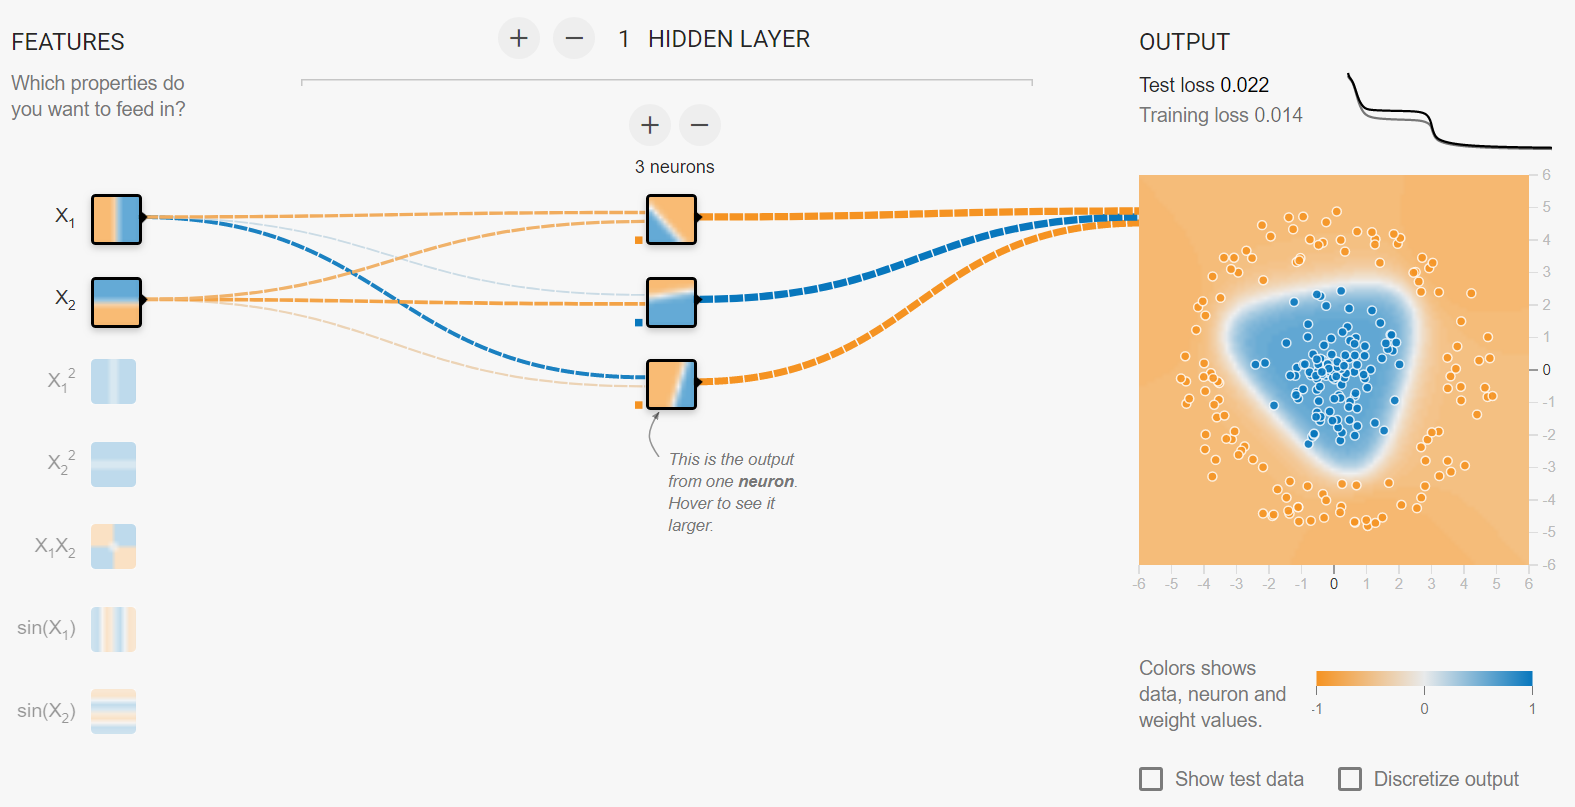
\includegraphics[width=1.0\textwidth]{images/simple_neuronal_network}
					\caption[Simple neuronal network with one hidden layer]{Simple neuronal network with one hidden layer\footnotemark}
					\label{fig:beispiel4}
				\end{figure}
				\footnotetext{Source: \url{http://playground.tensorflow.org/}}
		
			\subsubsection{Convolutional Neuronal Network}
				\noindent A neural network processes a vector. A convolutional neural network, on the other hand, can process a matrix. Describe more here. 
	
			\subsubsection{Transfer Learning}
	
				\noindent Explain here the technique of Convolutional Neuronal Networks.
			
				\paragraph{Transfer Learning Models}
		
					\hl{...}
			
					\begin{figure}[H]
						\centering
						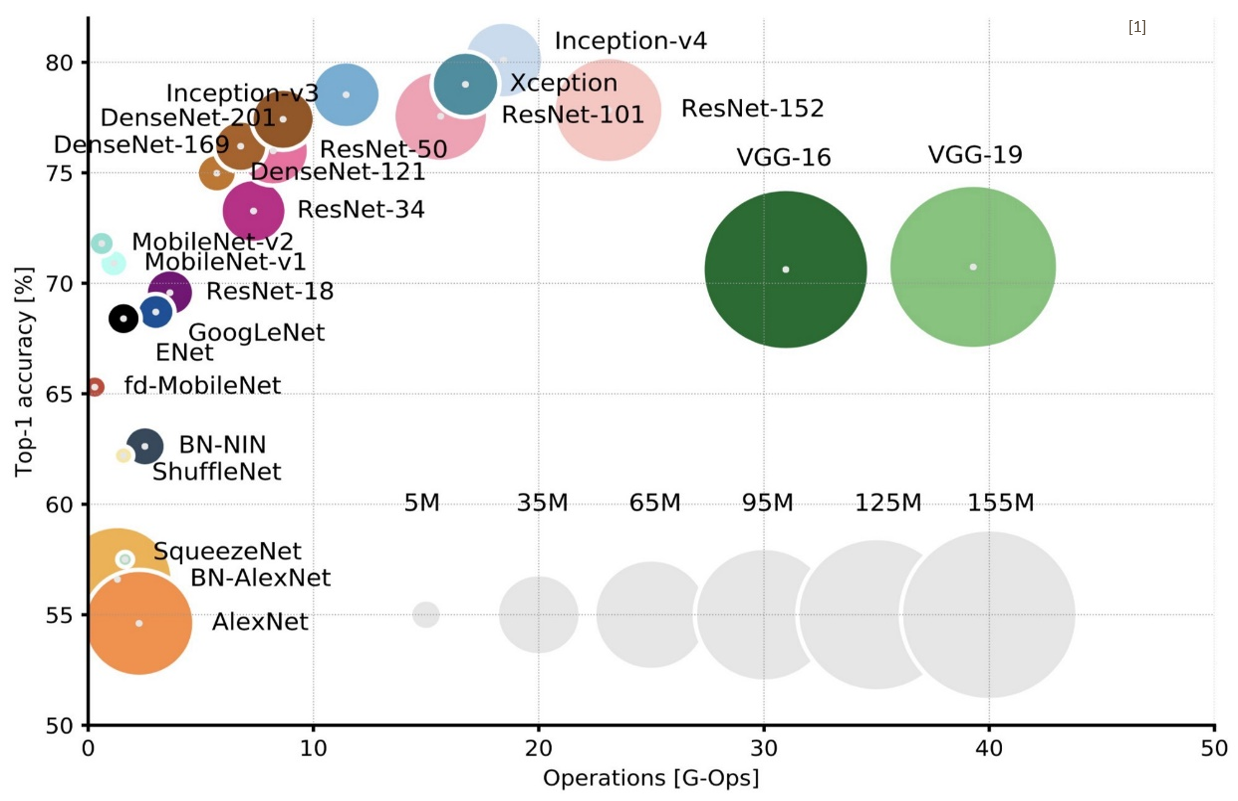
\includegraphics[width=1.0\textwidth]{images/tl_models}
						\caption[Overview of known transfer learning models.]{Overview of known transfer learning models.\footnotemark}
						\label{fig:beispiel5}
					\end{figure}
					\footnotetext{Source: \url{https://towardsdatascience.com/neural-network-architectures-156e5bad51ba}}
		
					\hl{...}
					
					
					
	% -------------------- %
	% Insufficient amount of data %
	% -------------------- %
	\section{Insufficient amount of data}
	\label{sec:section_insufficient_amount_of_data}
		\de{Gibt man einem Menschen einen Donut und erkärt ihm, dass es ein Donut ist, so ist dieser nach einigem Wiederholen selbstständig in der Lage diesen Donut in der Zukunft zu klassifizieren. Bei Machine Learning ist diese Problematik etwas komplexer. Wie bei den meisten machinellen Lernverfahren benötigt man eine große Menge an Daten. Wieviel ist nicht richtig belegt. Gerade wenn man es mit vielen vorherzusagenden Klassen zu tun hat, erhöht sich die Datenmenge erfahrungsgemäß. Einige Meinungen in Foren und Blogartikeln besagen (Hypothese), dass es mindestens 1000 Bilder pro Klasse sein müssen.\footnote{``Deep Learning for Image Classification with Less Data'', https://towardsdatascience.com, February 2, 2020, \url{https://towardsdatascience.com/deep-learning-for-image-classification-with-less-data-90e5df0a7b8e}}\textsuperscript{,}\footnote{``How many images do you need to train a neural network?'', https://petewarden.com, February 2, 2020, \url{https://petewarden.com/2017/12/14/how-many-images-do-you-need-to-train-a-neural-network/}}\textsuperscript{,}\footnote{``What is the minimum sample size required to train a Deep Learning model - CNN?'', https://www.researchgate.net, February 2, 2020, \url{https://www.researchgate.net/post/What_is_the_minimum_sample_size_required_to_train_a_Deep_Learning_model-CNN}}\textsuperscript{,}\autocite{krizhevsky2012imagenet}.}
		\en{If you give a person a donut and explain to him that it is a donut, then after some repetition he is able to classify this donut in the future. With Machine Learning this problem is a bit more complex. As with most machine learning methods, a large amount of data is required. How much is not properly documented. Especially when you are dealing with many classes to be predicted, experience shows that the amount of data increases. Some opinions in forums and blog articles say (hypothesis) that there must be at least 1000 pictures per class.\footnote{``Deep Learning for Image Classification with Less Data'', https://towardsdatascience.com, February 2, 2020, \url{https://towardsdatascience.com/deep-learning-for-image-classification-with-less-data-90e5df0a7b8e}}\textsuperscript{,}\footnote{``How many images do you need to train a neural network?'', https://petewarden.com, February 2, 2020, \url{https://petewarden.com/2017/12/14/how-many-images-do-you-need-to-train-a-neural-network/}}\textsuperscript{,}\footnote{``What is the minimum sample size required to train a Deep Learning model - CNN?'', https://www.researchgate.net, February 2, 2020, \url{https://www.researchgate.net/post/What_is_the_minimum_sample_size_required_to_train_a_Deep_Learning_model-CNN}}\textsuperscript{,}\autocite{krizhevsky2012imagenet}}

		\de{Je nach Anzahl von zu trainierenden Klassen gelangt man somit schnell zu einem benötigten Datenset, welches aus mehrere Gigabyte an Daten besteht. Mittels Transfer Learning ist es möglich diese Zahl nochmals etwas zu reduzieren, jedoch bleibt das Problem der vielen Daten bestehen. Ein Paper von Microsoft aus dem Jahre 2001 zeigte zur damaligen Zeit, dass einfache Algorithmen mit genügend Daten ähnliche Ergebnisse lieferten, wie komplexe Algorithmen auf Basis weniger Daten. Dabei bezogen sich die Forscher auf Daten, welche Sprachkonstrukte klassifizieren sollten:}
		\en{Depending on the number of classes to be trained, you will quickly arrive at the required data set, which consists of several gigabytes of data. With Transfer Learning it is possible to reduce this number a little bit, but the problem of the large amount of data remains. A paper  from Microsoft in 2001 showed at that time that simple algorithms with enough data gave similar results as complex algorithms based on less data. The researchers referred to data which should classify language constructs:}
		
		\blockquote{\textit{We have shown that for a prototypical natural language classification task, the performance of learners can benefit significantly from much larger training sets.}}\autocite{banko2001scaling}
		
		\de{In einem anderen Artikel nur wenige Jahre später wird dieses Thema ebenfalls aufgegriffen. Dabei bezog man sich auf Daten, welche von Texten lernen und man meist nur kleine oder mittelgroße Datensätze zur Verfügung hat. Um die Effizienz auch in diesem Fall zu verbessern, ist es eine gute Idee die Algorithmen und Methoden zu verbessern: \hl{Beispiele!}}
		\en{Another article only a few years later also addresses this issue. This referred to data that learn from texts and that usually only small or medium sized data sets are available. To improve the efficiency also in this case, it is a good idea to improve the algorithms and methods: \hl{Examples!}}

		\blockquote{\textit{...\autocite{halevy2009unreasonable}.}}



	% -------------------- %
	% Validation process %
	% -------------------- %
	\section{Related work}
		\hl{...}



	% -------------------- %
	% Validation process %
	% -------------------- %
	\section{Validation process}

		\hl{This is the part where I explain my approach.}
	
		\subsection{Preamble}
			In the following, the best possible accuracy is to be achieved by testing various parameters.
			A learning set with the following properties was used:
	
			\begin{itemize}
				\item 14865 images
				\item classified within 50 classes
				\item different number of images per class (unbalanced)
			\end{itemize}
	
			With the exception of the model tests, all tests were based on the following parameters
			(whereby one value of the parameters varied depending on the chapter):
		
			\begin{itemize}
				\item model: resnet18
				\item learning rate: 0,001 (decreases every 7 epochs to 10\% of the previous value)
				\item batch size: 48
				\item epochs: 21 (learning rate from epoch 15 to 21: 0,00001)
				\item image size: 224x224 pixels
				\item the entire training and validation set (14865 images)
			\end{itemize}
		
			Different models were tried out in chapter \flqq\nameref{usedModels}\footnote{
				see on page \pageref{usedModels}
				chapter \ref{usedModels}
				\flqq\nameref{usedModels}\frqq
			}\frqq{} with the same
			parameters as above:
		
			\begin{itemize}
				\item ResNet18
				\item ResNet50
				\item ResNet152
				\item AlexNet
				\item VGG
				\item SqueezeNet
				\item DenseNet
				\item Inception v3
			\end{itemize}
			
		\subsection{Working environment}
	
			\hl{Explain in this part of the thesis the frameworks, environments and hardware used, etc.}
			
		\subsection{Splitting and preparing the data}
		
			\subsubsection{Situation}
			
				We have 14866 images differently distributed in 50 classes (unbalanced). We would like to divide these into 80\% training and 20\% validation images.
				
			\subsubsection{Unbalanced}
			
				The unbalanced dispersion data set is divided exactly in the same ratio:
				
				\begin{itemize}
					\item 2953 images for the training
					\item 11913 images for validation
				\end{itemize}
				
				For training with different training elements, the validation dataset of 2953 images is retained for a comparable result. The number of training elements deviating from the total data set results from this:
				
				\begin{equation}
					n_{train} = k \cdot 500;  k \in 1 \dots 26
				\end{equation}
			
			\subsubsection{Balanced}
		
				\noindent ...
	
		\subsection{Performance}
		
			\noindent ...
		
		\pagebreak
	
		\subsection{Accuracy and evaluations}

			\noindent ...

			\subsubsection{Influence of number of trained images on accuracy}
	
				\noindent ...

				\begin{figure}[H]
					\begin{center}
						%% Creator: Matplotlib, PGF backend
%%
%% To include the figure in your LaTeX document, write
%%   \input{<filename>.pgf}
%%
%% Make sure the required packages are loaded in your preamble
%%   \usepackage{pgf}
%%
%% Figures using additional raster images can only be included by \input if
%% they are in the same directory as the main LaTeX file. For loading figures
%% from other directories you can use the `import` package
%%   \usepackage{import}
%% and then include the figures with
%%   \import{<path to file>}{<filename>.pgf}
%%
%% Matplotlib used the following preamble
%%   \usepackage{fontspec}
%%   \setmainfont{DejaVuSerif.ttf}[Path=C:/Users/bjoern/Anaconda3/envs/keras-gpu/lib/site-packages/matplotlib/mpl-data/fonts/ttf/]
%%   \setsansfont{DejaVuSans.ttf}[Path=C:/Users/bjoern/Anaconda3/envs/keras-gpu/lib/site-packages/matplotlib/mpl-data/fonts/ttf/]
%%   \setmonofont{DejaVuSansMono.ttf}[Path=C:/Users/bjoern/Anaconda3/envs/keras-gpu/lib/site-packages/matplotlib/mpl-data/fonts/ttf/]
%%
\begingroup%
\makeatletter%
\begin{pgfpicture}%
\pgfpathrectangle{\pgfpointorigin}{\pgfqpoint{6.000000in}{3.000000in}}%
\pgfusepath{use as bounding box, clip}%
\begin{pgfscope}%
\pgfsetbuttcap%
\pgfsetmiterjoin%
\definecolor{currentfill}{rgb}{1.000000,1.000000,1.000000}%
\pgfsetfillcolor{currentfill}%
\pgfsetlinewidth{0.000000pt}%
\definecolor{currentstroke}{rgb}{1.000000,1.000000,1.000000}%
\pgfsetstrokecolor{currentstroke}%
\pgfsetdash{}{0pt}%
\pgfpathmoveto{\pgfqpoint{0.000000in}{0.000000in}}%
\pgfpathlineto{\pgfqpoint{6.000000in}{0.000000in}}%
\pgfpathlineto{\pgfqpoint{6.000000in}{3.000000in}}%
\pgfpathlineto{\pgfqpoint{0.000000in}{3.000000in}}%
\pgfpathclose%
\pgfusepath{fill}%
\end{pgfscope}%
\begin{pgfscope}%
\pgfsetbuttcap%
\pgfsetmiterjoin%
\definecolor{currentfill}{rgb}{1.000000,1.000000,1.000000}%
\pgfsetfillcolor{currentfill}%
\pgfsetlinewidth{0.000000pt}%
\definecolor{currentstroke}{rgb}{0.000000,0.000000,0.000000}%
\pgfsetstrokecolor{currentstroke}%
\pgfsetstrokeopacity{0.000000}%
\pgfsetdash{}{0pt}%
\pgfpathmoveto{\pgfqpoint{0.720000in}{0.540000in}}%
\pgfpathlineto{\pgfqpoint{5.700000in}{0.540000in}}%
\pgfpathlineto{\pgfqpoint{5.700000in}{2.700000in}}%
\pgfpathlineto{\pgfqpoint{0.720000in}{2.700000in}}%
\pgfpathclose%
\pgfusepath{fill}%
\end{pgfscope}%
\begin{pgfscope}%
\pgfpathrectangle{\pgfqpoint{0.720000in}{0.540000in}}{\pgfqpoint{4.980000in}{2.160000in}}%
\pgfusepath{clip}%
\pgfsetrectcap%
\pgfsetroundjoin%
\pgfsetlinewidth{0.803000pt}%
\definecolor{currentstroke}{rgb}{0.690196,0.690196,0.690196}%
\pgfsetstrokecolor{currentstroke}%
\pgfsetdash{}{0pt}%
\pgfpathmoveto{\pgfqpoint{0.720000in}{0.540000in}}%
\pgfpathlineto{\pgfqpoint{0.720000in}{2.700000in}}%
\pgfusepath{stroke}%
\end{pgfscope}%
\begin{pgfscope}%
\pgfsetbuttcap%
\pgfsetroundjoin%
\definecolor{currentfill}{rgb}{0.000000,0.000000,0.000000}%
\pgfsetfillcolor{currentfill}%
\pgfsetlinewidth{0.803000pt}%
\definecolor{currentstroke}{rgb}{0.000000,0.000000,0.000000}%
\pgfsetstrokecolor{currentstroke}%
\pgfsetdash{}{0pt}%
\pgfsys@defobject{currentmarker}{\pgfqpoint{0.000000in}{-0.048611in}}{\pgfqpoint{0.000000in}{0.000000in}}{%
\pgfpathmoveto{\pgfqpoint{0.000000in}{0.000000in}}%
\pgfpathlineto{\pgfqpoint{0.000000in}{-0.048611in}}%
\pgfusepath{stroke,fill}%
}%
\begin{pgfscope}%
\pgfsys@transformshift{0.720000in}{0.540000in}%
\pgfsys@useobject{currentmarker}{}%
\end{pgfscope}%
\end{pgfscope}%
\begin{pgfscope}%
\definecolor{textcolor}{rgb}{0.000000,0.000000,0.000000}%
\pgfsetstrokecolor{textcolor}%
\pgfsetfillcolor{textcolor}%
\pgftext[x=0.720000in,y=0.442778in,,top]{\color{textcolor}\rmfamily\fontsize{8.000000}{9.600000}\selectfont 0 s}%
\end{pgfscope}%
\begin{pgfscope}%
\pgfpathrectangle{\pgfqpoint{0.720000in}{0.540000in}}{\pgfqpoint{4.980000in}{2.160000in}}%
\pgfusepath{clip}%
\pgfsetrectcap%
\pgfsetroundjoin%
\pgfsetlinewidth{0.803000pt}%
\definecolor{currentstroke}{rgb}{0.690196,0.690196,0.690196}%
\pgfsetstrokecolor{currentstroke}%
\pgfsetdash{}{0pt}%
\pgfpathmoveto{\pgfqpoint{2.380000in}{0.540000in}}%
\pgfpathlineto{\pgfqpoint{2.380000in}{2.700000in}}%
\pgfusepath{stroke}%
\end{pgfscope}%
\begin{pgfscope}%
\pgfsetbuttcap%
\pgfsetroundjoin%
\definecolor{currentfill}{rgb}{0.000000,0.000000,0.000000}%
\pgfsetfillcolor{currentfill}%
\pgfsetlinewidth{0.803000pt}%
\definecolor{currentstroke}{rgb}{0.000000,0.000000,0.000000}%
\pgfsetstrokecolor{currentstroke}%
\pgfsetdash{}{0pt}%
\pgfsys@defobject{currentmarker}{\pgfqpoint{0.000000in}{-0.048611in}}{\pgfqpoint{0.000000in}{0.000000in}}{%
\pgfpathmoveto{\pgfqpoint{0.000000in}{0.000000in}}%
\pgfpathlineto{\pgfqpoint{0.000000in}{-0.048611in}}%
\pgfusepath{stroke,fill}%
}%
\begin{pgfscope}%
\pgfsys@transformshift{2.380000in}{0.540000in}%
\pgfsys@useobject{currentmarker}{}%
\end{pgfscope}%
\end{pgfscope}%
\begin{pgfscope}%
\definecolor{textcolor}{rgb}{0.000000,0.000000,0.000000}%
\pgfsetstrokecolor{textcolor}%
\pgfsetfillcolor{textcolor}%
\pgftext[x=2.380000in,y=0.442778in,,top]{\color{textcolor}\rmfamily\fontsize{8.000000}{9.600000}\selectfont 3600 s}%
\end{pgfscope}%
\begin{pgfscope}%
\pgfpathrectangle{\pgfqpoint{0.720000in}{0.540000in}}{\pgfqpoint{4.980000in}{2.160000in}}%
\pgfusepath{clip}%
\pgfsetrectcap%
\pgfsetroundjoin%
\pgfsetlinewidth{0.803000pt}%
\definecolor{currentstroke}{rgb}{0.690196,0.690196,0.690196}%
\pgfsetstrokecolor{currentstroke}%
\pgfsetdash{}{0pt}%
\pgfpathmoveto{\pgfqpoint{4.040000in}{0.540000in}}%
\pgfpathlineto{\pgfqpoint{4.040000in}{2.700000in}}%
\pgfusepath{stroke}%
\end{pgfscope}%
\begin{pgfscope}%
\pgfsetbuttcap%
\pgfsetroundjoin%
\definecolor{currentfill}{rgb}{0.000000,0.000000,0.000000}%
\pgfsetfillcolor{currentfill}%
\pgfsetlinewidth{0.803000pt}%
\definecolor{currentstroke}{rgb}{0.000000,0.000000,0.000000}%
\pgfsetstrokecolor{currentstroke}%
\pgfsetdash{}{0pt}%
\pgfsys@defobject{currentmarker}{\pgfqpoint{0.000000in}{-0.048611in}}{\pgfqpoint{0.000000in}{0.000000in}}{%
\pgfpathmoveto{\pgfqpoint{0.000000in}{0.000000in}}%
\pgfpathlineto{\pgfqpoint{0.000000in}{-0.048611in}}%
\pgfusepath{stroke,fill}%
}%
\begin{pgfscope}%
\pgfsys@transformshift{4.040000in}{0.540000in}%
\pgfsys@useobject{currentmarker}{}%
\end{pgfscope}%
\end{pgfscope}%
\begin{pgfscope}%
\definecolor{textcolor}{rgb}{0.000000,0.000000,0.000000}%
\pgfsetstrokecolor{textcolor}%
\pgfsetfillcolor{textcolor}%
\pgftext[x=4.040000in,y=0.442778in,,top]{\color{textcolor}\rmfamily\fontsize{8.000000}{9.600000}\selectfont 7200 s}%
\end{pgfscope}%
\begin{pgfscope}%
\pgfpathrectangle{\pgfqpoint{0.720000in}{0.540000in}}{\pgfqpoint{4.980000in}{2.160000in}}%
\pgfusepath{clip}%
\pgfsetrectcap%
\pgfsetroundjoin%
\pgfsetlinewidth{0.803000pt}%
\definecolor{currentstroke}{rgb}{0.690196,0.690196,0.690196}%
\pgfsetstrokecolor{currentstroke}%
\pgfsetdash{}{0pt}%
\pgfpathmoveto{\pgfqpoint{5.700000in}{0.540000in}}%
\pgfpathlineto{\pgfqpoint{5.700000in}{2.700000in}}%
\pgfusepath{stroke}%
\end{pgfscope}%
\begin{pgfscope}%
\pgfsetbuttcap%
\pgfsetroundjoin%
\definecolor{currentfill}{rgb}{0.000000,0.000000,0.000000}%
\pgfsetfillcolor{currentfill}%
\pgfsetlinewidth{0.803000pt}%
\definecolor{currentstroke}{rgb}{0.000000,0.000000,0.000000}%
\pgfsetstrokecolor{currentstroke}%
\pgfsetdash{}{0pt}%
\pgfsys@defobject{currentmarker}{\pgfqpoint{0.000000in}{-0.048611in}}{\pgfqpoint{0.000000in}{0.000000in}}{%
\pgfpathmoveto{\pgfqpoint{0.000000in}{0.000000in}}%
\pgfpathlineto{\pgfqpoint{0.000000in}{-0.048611in}}%
\pgfusepath{stroke,fill}%
}%
\begin{pgfscope}%
\pgfsys@transformshift{5.700000in}{0.540000in}%
\pgfsys@useobject{currentmarker}{}%
\end{pgfscope}%
\end{pgfscope}%
\begin{pgfscope}%
\definecolor{textcolor}{rgb}{0.000000,0.000000,0.000000}%
\pgfsetstrokecolor{textcolor}%
\pgfsetfillcolor{textcolor}%
\pgftext[x=5.700000in,y=0.442778in,,top]{\color{textcolor}\rmfamily\fontsize{8.000000}{9.600000}\selectfont 10800 s}%
\end{pgfscope}%
\begin{pgfscope}%
\definecolor{textcolor}{rgb}{0.000000,0.000000,0.000000}%
\pgfsetstrokecolor{textcolor}%
\pgfsetfillcolor{textcolor}%
\pgftext[x=3.210000in,y=0.279692in,,top]{\color{textcolor}\rmfamily\fontsize{10.000000}{12.000000}\selectfont model training time}%
\end{pgfscope}%
\begin{pgfscope}%
\pgfpathrectangle{\pgfqpoint{0.720000in}{0.540000in}}{\pgfqpoint{4.980000in}{2.160000in}}%
\pgfusepath{clip}%
\pgfsetrectcap%
\pgfsetroundjoin%
\pgfsetlinewidth{0.803000pt}%
\definecolor{currentstroke}{rgb}{0.690196,0.690196,0.690196}%
\pgfsetstrokecolor{currentstroke}%
\pgfsetdash{}{0pt}%
\pgfpathmoveto{\pgfqpoint{0.720000in}{0.940000in}}%
\pgfpathlineto{\pgfqpoint{5.700000in}{0.940000in}}%
\pgfusepath{stroke}%
\end{pgfscope}%
\begin{pgfscope}%
\pgfsetbuttcap%
\pgfsetroundjoin%
\definecolor{currentfill}{rgb}{0.000000,0.000000,0.000000}%
\pgfsetfillcolor{currentfill}%
\pgfsetlinewidth{0.803000pt}%
\definecolor{currentstroke}{rgb}{0.000000,0.000000,0.000000}%
\pgfsetstrokecolor{currentstroke}%
\pgfsetdash{}{0pt}%
\pgfsys@defobject{currentmarker}{\pgfqpoint{-0.048611in}{0.000000in}}{\pgfqpoint{0.000000in}{0.000000in}}{%
\pgfpathmoveto{\pgfqpoint{0.000000in}{0.000000in}}%
\pgfpathlineto{\pgfqpoint{-0.048611in}{0.000000in}}%
\pgfusepath{stroke,fill}%
}%
\begin{pgfscope}%
\pgfsys@transformshift{0.720000in}{0.940000in}%
\pgfsys@useobject{currentmarker}{}%
\end{pgfscope}%
\end{pgfscope}%
\begin{pgfscope}%
\definecolor{textcolor}{rgb}{0.000000,0.000000,0.000000}%
\pgfsetstrokecolor{textcolor}%
\pgfsetfillcolor{textcolor}%
\pgftext[x=0.375816in,y=0.897791in,left,base]{\color{textcolor}\rmfamily\fontsize{8.000000}{9.600000}\selectfont 20\%}%
\end{pgfscope}%
\begin{pgfscope}%
\pgfpathrectangle{\pgfqpoint{0.720000in}{0.540000in}}{\pgfqpoint{4.980000in}{2.160000in}}%
\pgfusepath{clip}%
\pgfsetrectcap%
\pgfsetroundjoin%
\pgfsetlinewidth{0.803000pt}%
\definecolor{currentstroke}{rgb}{0.690196,0.690196,0.690196}%
\pgfsetstrokecolor{currentstroke}%
\pgfsetdash{}{0pt}%
\pgfpathmoveto{\pgfqpoint{0.720000in}{1.473333in}}%
\pgfpathlineto{\pgfqpoint{5.700000in}{1.473333in}}%
\pgfusepath{stroke}%
\end{pgfscope}%
\begin{pgfscope}%
\pgfsetbuttcap%
\pgfsetroundjoin%
\definecolor{currentfill}{rgb}{0.000000,0.000000,0.000000}%
\pgfsetfillcolor{currentfill}%
\pgfsetlinewidth{0.803000pt}%
\definecolor{currentstroke}{rgb}{0.000000,0.000000,0.000000}%
\pgfsetstrokecolor{currentstroke}%
\pgfsetdash{}{0pt}%
\pgfsys@defobject{currentmarker}{\pgfqpoint{-0.048611in}{0.000000in}}{\pgfqpoint{0.000000in}{0.000000in}}{%
\pgfpathmoveto{\pgfqpoint{0.000000in}{0.000000in}}%
\pgfpathlineto{\pgfqpoint{-0.048611in}{0.000000in}}%
\pgfusepath{stroke,fill}%
}%
\begin{pgfscope}%
\pgfsys@transformshift{0.720000in}{1.473333in}%
\pgfsys@useobject{currentmarker}{}%
\end{pgfscope}%
\end{pgfscope}%
\begin{pgfscope}%
\definecolor{textcolor}{rgb}{0.000000,0.000000,0.000000}%
\pgfsetstrokecolor{textcolor}%
\pgfsetfillcolor{textcolor}%
\pgftext[x=0.375816in,y=1.431124in,left,base]{\color{textcolor}\rmfamily\fontsize{8.000000}{9.600000}\selectfont 40\%}%
\end{pgfscope}%
\begin{pgfscope}%
\pgfpathrectangle{\pgfqpoint{0.720000in}{0.540000in}}{\pgfqpoint{4.980000in}{2.160000in}}%
\pgfusepath{clip}%
\pgfsetrectcap%
\pgfsetroundjoin%
\pgfsetlinewidth{0.803000pt}%
\definecolor{currentstroke}{rgb}{0.690196,0.690196,0.690196}%
\pgfsetstrokecolor{currentstroke}%
\pgfsetdash{}{0pt}%
\pgfpathmoveto{\pgfqpoint{0.720000in}{2.006667in}}%
\pgfpathlineto{\pgfqpoint{5.700000in}{2.006667in}}%
\pgfusepath{stroke}%
\end{pgfscope}%
\begin{pgfscope}%
\pgfsetbuttcap%
\pgfsetroundjoin%
\definecolor{currentfill}{rgb}{0.000000,0.000000,0.000000}%
\pgfsetfillcolor{currentfill}%
\pgfsetlinewidth{0.803000pt}%
\definecolor{currentstroke}{rgb}{0.000000,0.000000,0.000000}%
\pgfsetstrokecolor{currentstroke}%
\pgfsetdash{}{0pt}%
\pgfsys@defobject{currentmarker}{\pgfqpoint{-0.048611in}{0.000000in}}{\pgfqpoint{0.000000in}{0.000000in}}{%
\pgfpathmoveto{\pgfqpoint{0.000000in}{0.000000in}}%
\pgfpathlineto{\pgfqpoint{-0.048611in}{0.000000in}}%
\pgfusepath{stroke,fill}%
}%
\begin{pgfscope}%
\pgfsys@transformshift{0.720000in}{2.006667in}%
\pgfsys@useobject{currentmarker}{}%
\end{pgfscope}%
\end{pgfscope}%
\begin{pgfscope}%
\definecolor{textcolor}{rgb}{0.000000,0.000000,0.000000}%
\pgfsetstrokecolor{textcolor}%
\pgfsetfillcolor{textcolor}%
\pgftext[x=0.375816in,y=1.964457in,left,base]{\color{textcolor}\rmfamily\fontsize{8.000000}{9.600000}\selectfont 60\%}%
\end{pgfscope}%
\begin{pgfscope}%
\pgfpathrectangle{\pgfqpoint{0.720000in}{0.540000in}}{\pgfqpoint{4.980000in}{2.160000in}}%
\pgfusepath{clip}%
\pgfsetrectcap%
\pgfsetroundjoin%
\pgfsetlinewidth{0.803000pt}%
\definecolor{currentstroke}{rgb}{0.690196,0.690196,0.690196}%
\pgfsetstrokecolor{currentstroke}%
\pgfsetdash{}{0pt}%
\pgfpathmoveto{\pgfqpoint{0.720000in}{2.540000in}}%
\pgfpathlineto{\pgfqpoint{5.700000in}{2.540000in}}%
\pgfusepath{stroke}%
\end{pgfscope}%
\begin{pgfscope}%
\pgfsetbuttcap%
\pgfsetroundjoin%
\definecolor{currentfill}{rgb}{0.000000,0.000000,0.000000}%
\pgfsetfillcolor{currentfill}%
\pgfsetlinewidth{0.803000pt}%
\definecolor{currentstroke}{rgb}{0.000000,0.000000,0.000000}%
\pgfsetstrokecolor{currentstroke}%
\pgfsetdash{}{0pt}%
\pgfsys@defobject{currentmarker}{\pgfqpoint{-0.048611in}{0.000000in}}{\pgfqpoint{0.000000in}{0.000000in}}{%
\pgfpathmoveto{\pgfqpoint{0.000000in}{0.000000in}}%
\pgfpathlineto{\pgfqpoint{-0.048611in}{0.000000in}}%
\pgfusepath{stroke,fill}%
}%
\begin{pgfscope}%
\pgfsys@transformshift{0.720000in}{2.540000in}%
\pgfsys@useobject{currentmarker}{}%
\end{pgfscope}%
\end{pgfscope}%
\begin{pgfscope}%
\definecolor{textcolor}{rgb}{0.000000,0.000000,0.000000}%
\pgfsetstrokecolor{textcolor}%
\pgfsetfillcolor{textcolor}%
\pgftext[x=0.375816in,y=2.497791in,left,base]{\color{textcolor}\rmfamily\fontsize{8.000000}{9.600000}\selectfont 80\%}%
\end{pgfscope}%
\begin{pgfscope}%
\definecolor{textcolor}{rgb}{0.000000,0.000000,0.000000}%
\pgfsetstrokecolor{textcolor}%
\pgfsetfillcolor{textcolor}%
\pgftext[x=0.320260in,y=1.620000in,,bottom,rotate=90.000000]{\color{textcolor}\rmfamily\fontsize{10.000000}{12.000000}\selectfont accuracy validation top-1}%
\end{pgfscope}%
\begin{pgfscope}%
\pgfpathrectangle{\pgfqpoint{0.720000in}{0.540000in}}{\pgfqpoint{4.980000in}{2.160000in}}%
\pgfusepath{clip}%
\pgfsetrectcap%
\pgfsetroundjoin%
\pgfsetlinewidth{0.752812pt}%
\definecolor{currentstroke}{rgb}{0.000000,0.000000,1.000000}%
\pgfsetstrokecolor{currentstroke}%
\pgfsetdash{}{0pt}%
\pgfpathmoveto{\pgfqpoint{0.750894in}{0.571467in}}%
\pgfpathlineto{\pgfqpoint{0.774411in}{0.731733in}}%
\pgfpathlineto{\pgfqpoint{0.797006in}{0.941333in}}%
\pgfpathlineto{\pgfqpoint{0.819600in}{1.053067in}}%
\pgfpathlineto{\pgfqpoint{0.842194in}{1.189333in}}%
\pgfpathlineto{\pgfqpoint{0.872167in}{1.206667in}}%
\pgfpathlineto{\pgfqpoint{0.894761in}{1.321867in}}%
\pgfpathlineto{\pgfqpoint{0.917356in}{1.435467in}}%
\pgfpathlineto{\pgfqpoint{0.939950in}{1.497067in}}%
\pgfpathlineto{\pgfqpoint{0.962544in}{1.458133in}}%
\pgfpathlineto{\pgfqpoint{0.985139in}{1.516267in}}%
\pgfpathlineto{\pgfqpoint{1.007733in}{1.564267in}}%
\pgfpathlineto{\pgfqpoint{1.030328in}{1.512533in}}%
\pgfpathlineto{\pgfqpoint{1.052922in}{1.549867in}}%
\pgfpathlineto{\pgfqpoint{1.075517in}{1.603467in}}%
\pgfpathlineto{\pgfqpoint{1.098111in}{1.584267in}}%
\pgfpathlineto{\pgfqpoint{1.120706in}{1.618667in}}%
\pgfpathlineto{\pgfqpoint{1.143300in}{1.578933in}}%
\pgfpathlineto{\pgfqpoint{1.165894in}{1.616000in}}%
\pgfpathlineto{\pgfqpoint{1.188489in}{1.626933in}}%
\pgfpathlineto{\pgfqpoint{1.211083in}{1.617067in}}%
\pgfusepath{stroke}%
\end{pgfscope}%
\begin{pgfscope}%
\pgfpathrectangle{\pgfqpoint{0.720000in}{0.540000in}}{\pgfqpoint{4.980000in}{2.160000in}}%
\pgfusepath{clip}%
\pgfsetbuttcap%
\pgfsetroundjoin%
\definecolor{currentfill}{rgb}{0.000000,0.000000,1.000000}%
\pgfsetfillcolor{currentfill}%
\pgfsetlinewidth{1.003750pt}%
\definecolor{currentstroke}{rgb}{0.000000,0.000000,1.000000}%
\pgfsetstrokecolor{currentstroke}%
\pgfsetdash{}{0pt}%
\pgfsys@defobject{currentmarker}{\pgfqpoint{-0.010417in}{-0.010417in}}{\pgfqpoint{0.010417in}{0.010417in}}{%
\pgfpathmoveto{\pgfqpoint{0.000000in}{-0.010417in}}%
\pgfpathcurveto{\pgfqpoint{0.002763in}{-0.010417in}}{\pgfqpoint{0.005412in}{-0.009319in}}{\pgfqpoint{0.007366in}{-0.007366in}}%
\pgfpathcurveto{\pgfqpoint{0.009319in}{-0.005412in}}{\pgfqpoint{0.010417in}{-0.002763in}}{\pgfqpoint{0.010417in}{0.000000in}}%
\pgfpathcurveto{\pgfqpoint{0.010417in}{0.002763in}}{\pgfqpoint{0.009319in}{0.005412in}}{\pgfqpoint{0.007366in}{0.007366in}}%
\pgfpathcurveto{\pgfqpoint{0.005412in}{0.009319in}}{\pgfqpoint{0.002763in}{0.010417in}}{\pgfqpoint{0.000000in}{0.010417in}}%
\pgfpathcurveto{\pgfqpoint{-0.002763in}{0.010417in}}{\pgfqpoint{-0.005412in}{0.009319in}}{\pgfqpoint{-0.007366in}{0.007366in}}%
\pgfpathcurveto{\pgfqpoint{-0.009319in}{0.005412in}}{\pgfqpoint{-0.010417in}{0.002763in}}{\pgfqpoint{-0.010417in}{0.000000in}}%
\pgfpathcurveto{\pgfqpoint{-0.010417in}{-0.002763in}}{\pgfqpoint{-0.009319in}{-0.005412in}}{\pgfqpoint{-0.007366in}{-0.007366in}}%
\pgfpathcurveto{\pgfqpoint{-0.005412in}{-0.009319in}}{\pgfqpoint{-0.002763in}{-0.010417in}}{\pgfqpoint{0.000000in}{-0.010417in}}%
\pgfpathclose%
\pgfusepath{stroke,fill}%
}%
\begin{pgfscope}%
\pgfsys@transformshift{0.750894in}{0.571467in}%
\pgfsys@useobject{currentmarker}{}%
\end{pgfscope}%
\begin{pgfscope}%
\pgfsys@transformshift{0.774411in}{0.731733in}%
\pgfsys@useobject{currentmarker}{}%
\end{pgfscope}%
\begin{pgfscope}%
\pgfsys@transformshift{0.797006in}{0.941333in}%
\pgfsys@useobject{currentmarker}{}%
\end{pgfscope}%
\begin{pgfscope}%
\pgfsys@transformshift{0.819600in}{1.053067in}%
\pgfsys@useobject{currentmarker}{}%
\end{pgfscope}%
\begin{pgfscope}%
\pgfsys@transformshift{0.842194in}{1.189333in}%
\pgfsys@useobject{currentmarker}{}%
\end{pgfscope}%
\begin{pgfscope}%
\pgfsys@transformshift{0.872167in}{1.206667in}%
\pgfsys@useobject{currentmarker}{}%
\end{pgfscope}%
\begin{pgfscope}%
\pgfsys@transformshift{0.894761in}{1.321867in}%
\pgfsys@useobject{currentmarker}{}%
\end{pgfscope}%
\begin{pgfscope}%
\pgfsys@transformshift{0.917356in}{1.435467in}%
\pgfsys@useobject{currentmarker}{}%
\end{pgfscope}%
\begin{pgfscope}%
\pgfsys@transformshift{0.939950in}{1.497067in}%
\pgfsys@useobject{currentmarker}{}%
\end{pgfscope}%
\begin{pgfscope}%
\pgfsys@transformshift{0.962544in}{1.458133in}%
\pgfsys@useobject{currentmarker}{}%
\end{pgfscope}%
\begin{pgfscope}%
\pgfsys@transformshift{0.985139in}{1.516267in}%
\pgfsys@useobject{currentmarker}{}%
\end{pgfscope}%
\begin{pgfscope}%
\pgfsys@transformshift{1.007733in}{1.564267in}%
\pgfsys@useobject{currentmarker}{}%
\end{pgfscope}%
\begin{pgfscope}%
\pgfsys@transformshift{1.030328in}{1.512533in}%
\pgfsys@useobject{currentmarker}{}%
\end{pgfscope}%
\begin{pgfscope}%
\pgfsys@transformshift{1.052922in}{1.549867in}%
\pgfsys@useobject{currentmarker}{}%
\end{pgfscope}%
\begin{pgfscope}%
\pgfsys@transformshift{1.075517in}{1.603467in}%
\pgfsys@useobject{currentmarker}{}%
\end{pgfscope}%
\begin{pgfscope}%
\pgfsys@transformshift{1.098111in}{1.584267in}%
\pgfsys@useobject{currentmarker}{}%
\end{pgfscope}%
\begin{pgfscope}%
\pgfsys@transformshift{1.120706in}{1.618667in}%
\pgfsys@useobject{currentmarker}{}%
\end{pgfscope}%
\begin{pgfscope}%
\pgfsys@transformshift{1.143300in}{1.578933in}%
\pgfsys@useobject{currentmarker}{}%
\end{pgfscope}%
\begin{pgfscope}%
\pgfsys@transformshift{1.165894in}{1.616000in}%
\pgfsys@useobject{currentmarker}{}%
\end{pgfscope}%
\begin{pgfscope}%
\pgfsys@transformshift{1.188489in}{1.626933in}%
\pgfsys@useobject{currentmarker}{}%
\end{pgfscope}%
\begin{pgfscope}%
\pgfsys@transformshift{1.211083in}{1.617067in}%
\pgfsys@useobject{currentmarker}{}%
\end{pgfscope}%
\end{pgfscope}%
\begin{pgfscope}%
\pgfpathrectangle{\pgfqpoint{0.720000in}{0.540000in}}{\pgfqpoint{4.980000in}{2.160000in}}%
\pgfusepath{clip}%
\pgfsetrectcap%
\pgfsetroundjoin%
\pgfsetlinewidth{0.752812pt}%
\definecolor{currentstroke}{rgb}{1.000000,0.647059,0.000000}%
\pgfsetstrokecolor{currentstroke}%
\pgfsetdash{}{0pt}%
\pgfpathmoveto{\pgfqpoint{0.757811in}{0.797067in}}%
\pgfpathlineto{\pgfqpoint{0.789167in}{1.142133in}}%
\pgfpathlineto{\pgfqpoint{0.819600in}{1.458133in}}%
\pgfpathlineto{\pgfqpoint{0.850033in}{1.633333in}}%
\pgfpathlineto{\pgfqpoint{0.880467in}{1.791200in}}%
\pgfpathlineto{\pgfqpoint{0.910900in}{1.886667in}}%
\pgfpathlineto{\pgfqpoint{0.941333in}{1.885600in}}%
\pgfpathlineto{\pgfqpoint{0.971767in}{1.943733in}}%
\pgfpathlineto{\pgfqpoint{1.002200in}{1.965600in}}%
\pgfpathlineto{\pgfqpoint{1.032633in}{2.012000in}}%
\pgfpathlineto{\pgfqpoint{1.063067in}{2.021867in}}%
\pgfpathlineto{\pgfqpoint{1.093500in}{2.030133in}}%
\pgfpathlineto{\pgfqpoint{1.123933in}{2.013867in}}%
\pgfpathlineto{\pgfqpoint{1.154367in}{1.997333in}}%
\pgfpathlineto{\pgfqpoint{1.184800in}{2.021867in}}%
\pgfpathlineto{\pgfqpoint{1.215233in}{2.027467in}}%
\pgfpathlineto{\pgfqpoint{1.245667in}{2.029067in}}%
\pgfpathlineto{\pgfqpoint{1.276100in}{2.044533in}}%
\pgfpathlineto{\pgfqpoint{1.306533in}{2.041867in}}%
\pgfpathlineto{\pgfqpoint{1.336967in}{2.037333in}}%
\pgfpathlineto{\pgfqpoint{1.367400in}{1.999200in}}%
\pgfusepath{stroke}%
\end{pgfscope}%
\begin{pgfscope}%
\pgfpathrectangle{\pgfqpoint{0.720000in}{0.540000in}}{\pgfqpoint{4.980000in}{2.160000in}}%
\pgfusepath{clip}%
\pgfsetbuttcap%
\pgfsetroundjoin%
\definecolor{currentfill}{rgb}{1.000000,0.647059,0.000000}%
\pgfsetfillcolor{currentfill}%
\pgfsetlinewidth{1.003750pt}%
\definecolor{currentstroke}{rgb}{1.000000,0.647059,0.000000}%
\pgfsetstrokecolor{currentstroke}%
\pgfsetdash{}{0pt}%
\pgfsys@defobject{currentmarker}{\pgfqpoint{-0.010417in}{-0.010417in}}{\pgfqpoint{0.010417in}{0.010417in}}{%
\pgfpathmoveto{\pgfqpoint{0.000000in}{-0.010417in}}%
\pgfpathcurveto{\pgfqpoint{0.002763in}{-0.010417in}}{\pgfqpoint{0.005412in}{-0.009319in}}{\pgfqpoint{0.007366in}{-0.007366in}}%
\pgfpathcurveto{\pgfqpoint{0.009319in}{-0.005412in}}{\pgfqpoint{0.010417in}{-0.002763in}}{\pgfqpoint{0.010417in}{0.000000in}}%
\pgfpathcurveto{\pgfqpoint{0.010417in}{0.002763in}}{\pgfqpoint{0.009319in}{0.005412in}}{\pgfqpoint{0.007366in}{0.007366in}}%
\pgfpathcurveto{\pgfqpoint{0.005412in}{0.009319in}}{\pgfqpoint{0.002763in}{0.010417in}}{\pgfqpoint{0.000000in}{0.010417in}}%
\pgfpathcurveto{\pgfqpoint{-0.002763in}{0.010417in}}{\pgfqpoint{-0.005412in}{0.009319in}}{\pgfqpoint{-0.007366in}{0.007366in}}%
\pgfpathcurveto{\pgfqpoint{-0.009319in}{0.005412in}}{\pgfqpoint{-0.010417in}{0.002763in}}{\pgfqpoint{-0.010417in}{0.000000in}}%
\pgfpathcurveto{\pgfqpoint{-0.010417in}{-0.002763in}}{\pgfqpoint{-0.009319in}{-0.005412in}}{\pgfqpoint{-0.007366in}{-0.007366in}}%
\pgfpathcurveto{\pgfqpoint{-0.005412in}{-0.009319in}}{\pgfqpoint{-0.002763in}{-0.010417in}}{\pgfqpoint{0.000000in}{-0.010417in}}%
\pgfpathclose%
\pgfusepath{stroke,fill}%
}%
\begin{pgfscope}%
\pgfsys@transformshift{0.757811in}{0.797067in}%
\pgfsys@useobject{currentmarker}{}%
\end{pgfscope}%
\begin{pgfscope}%
\pgfsys@transformshift{0.789167in}{1.142133in}%
\pgfsys@useobject{currentmarker}{}%
\end{pgfscope}%
\begin{pgfscope}%
\pgfsys@transformshift{0.819600in}{1.458133in}%
\pgfsys@useobject{currentmarker}{}%
\end{pgfscope}%
\begin{pgfscope}%
\pgfsys@transformshift{0.850033in}{1.633333in}%
\pgfsys@useobject{currentmarker}{}%
\end{pgfscope}%
\begin{pgfscope}%
\pgfsys@transformshift{0.880467in}{1.791200in}%
\pgfsys@useobject{currentmarker}{}%
\end{pgfscope}%
\begin{pgfscope}%
\pgfsys@transformshift{0.910900in}{1.886667in}%
\pgfsys@useobject{currentmarker}{}%
\end{pgfscope}%
\begin{pgfscope}%
\pgfsys@transformshift{0.941333in}{1.885600in}%
\pgfsys@useobject{currentmarker}{}%
\end{pgfscope}%
\begin{pgfscope}%
\pgfsys@transformshift{0.971767in}{1.943733in}%
\pgfsys@useobject{currentmarker}{}%
\end{pgfscope}%
\begin{pgfscope}%
\pgfsys@transformshift{1.002200in}{1.965600in}%
\pgfsys@useobject{currentmarker}{}%
\end{pgfscope}%
\begin{pgfscope}%
\pgfsys@transformshift{1.032633in}{2.012000in}%
\pgfsys@useobject{currentmarker}{}%
\end{pgfscope}%
\begin{pgfscope}%
\pgfsys@transformshift{1.063067in}{2.021867in}%
\pgfsys@useobject{currentmarker}{}%
\end{pgfscope}%
\begin{pgfscope}%
\pgfsys@transformshift{1.093500in}{2.030133in}%
\pgfsys@useobject{currentmarker}{}%
\end{pgfscope}%
\begin{pgfscope}%
\pgfsys@transformshift{1.123933in}{2.013867in}%
\pgfsys@useobject{currentmarker}{}%
\end{pgfscope}%
\begin{pgfscope}%
\pgfsys@transformshift{1.154367in}{1.997333in}%
\pgfsys@useobject{currentmarker}{}%
\end{pgfscope}%
\begin{pgfscope}%
\pgfsys@transformshift{1.184800in}{2.021867in}%
\pgfsys@useobject{currentmarker}{}%
\end{pgfscope}%
\begin{pgfscope}%
\pgfsys@transformshift{1.215233in}{2.027467in}%
\pgfsys@useobject{currentmarker}{}%
\end{pgfscope}%
\begin{pgfscope}%
\pgfsys@transformshift{1.245667in}{2.029067in}%
\pgfsys@useobject{currentmarker}{}%
\end{pgfscope}%
\begin{pgfscope}%
\pgfsys@transformshift{1.276100in}{2.044533in}%
\pgfsys@useobject{currentmarker}{}%
\end{pgfscope}%
\begin{pgfscope}%
\pgfsys@transformshift{1.306533in}{2.041867in}%
\pgfsys@useobject{currentmarker}{}%
\end{pgfscope}%
\begin{pgfscope}%
\pgfsys@transformshift{1.336967in}{2.037333in}%
\pgfsys@useobject{currentmarker}{}%
\end{pgfscope}%
\begin{pgfscope}%
\pgfsys@transformshift{1.367400in}{1.999200in}%
\pgfsys@useobject{currentmarker}{}%
\end{pgfscope}%
\end{pgfscope}%
\begin{pgfscope}%
\pgfpathrectangle{\pgfqpoint{0.720000in}{0.540000in}}{\pgfqpoint{4.980000in}{2.160000in}}%
\pgfusepath{clip}%
\pgfsetrectcap%
\pgfsetroundjoin%
\pgfsetlinewidth{0.752812pt}%
\definecolor{currentstroke}{rgb}{0.000000,0.501961,0.000000}%
\pgfsetstrokecolor{currentstroke}%
\pgfsetdash{}{0pt}%
\pgfpathmoveto{\pgfqpoint{0.773028in}{1.198400in}}%
\pgfpathlineto{\pgfqpoint{0.818678in}{1.672267in}}%
\pgfpathlineto{\pgfqpoint{0.864328in}{1.970133in}}%
\pgfpathlineto{\pgfqpoint{0.909978in}{2.064533in}}%
\pgfpathlineto{\pgfqpoint{0.955628in}{2.140800in}}%
\pgfpathlineto{\pgfqpoint{1.001278in}{2.151733in}}%
\pgfpathlineto{\pgfqpoint{1.046928in}{2.197067in}}%
\pgfpathlineto{\pgfqpoint{1.092578in}{2.239733in}}%
\pgfpathlineto{\pgfqpoint{1.138228in}{2.252533in}}%
\pgfpathlineto{\pgfqpoint{1.183878in}{2.236267in}}%
\pgfpathlineto{\pgfqpoint{1.229528in}{2.242667in}}%
\pgfpathlineto{\pgfqpoint{1.275178in}{2.264267in}}%
\pgfpathlineto{\pgfqpoint{1.320828in}{2.262400in}}%
\pgfpathlineto{\pgfqpoint{1.366017in}{2.285333in}}%
\pgfpathlineto{\pgfqpoint{1.411667in}{2.288000in}}%
\pgfpathlineto{\pgfqpoint{1.457317in}{2.274400in}}%
\pgfpathlineto{\pgfqpoint{1.502967in}{2.278933in}}%
\pgfpathlineto{\pgfqpoint{1.548617in}{2.273333in}}%
\pgfpathlineto{\pgfqpoint{1.594267in}{2.292533in}}%
\pgfpathlineto{\pgfqpoint{1.639917in}{2.284267in}}%
\pgfpathlineto{\pgfqpoint{1.685567in}{2.280800in}}%
\pgfusepath{stroke}%
\end{pgfscope}%
\begin{pgfscope}%
\pgfpathrectangle{\pgfqpoint{0.720000in}{0.540000in}}{\pgfqpoint{4.980000in}{2.160000in}}%
\pgfusepath{clip}%
\pgfsetbuttcap%
\pgfsetroundjoin%
\definecolor{currentfill}{rgb}{0.000000,0.501961,0.000000}%
\pgfsetfillcolor{currentfill}%
\pgfsetlinewidth{1.003750pt}%
\definecolor{currentstroke}{rgb}{0.000000,0.501961,0.000000}%
\pgfsetstrokecolor{currentstroke}%
\pgfsetdash{}{0pt}%
\pgfsys@defobject{currentmarker}{\pgfqpoint{-0.010417in}{-0.010417in}}{\pgfqpoint{0.010417in}{0.010417in}}{%
\pgfpathmoveto{\pgfqpoint{0.000000in}{-0.010417in}}%
\pgfpathcurveto{\pgfqpoint{0.002763in}{-0.010417in}}{\pgfqpoint{0.005412in}{-0.009319in}}{\pgfqpoint{0.007366in}{-0.007366in}}%
\pgfpathcurveto{\pgfqpoint{0.009319in}{-0.005412in}}{\pgfqpoint{0.010417in}{-0.002763in}}{\pgfqpoint{0.010417in}{0.000000in}}%
\pgfpathcurveto{\pgfqpoint{0.010417in}{0.002763in}}{\pgfqpoint{0.009319in}{0.005412in}}{\pgfqpoint{0.007366in}{0.007366in}}%
\pgfpathcurveto{\pgfqpoint{0.005412in}{0.009319in}}{\pgfqpoint{0.002763in}{0.010417in}}{\pgfqpoint{0.000000in}{0.010417in}}%
\pgfpathcurveto{\pgfqpoint{-0.002763in}{0.010417in}}{\pgfqpoint{-0.005412in}{0.009319in}}{\pgfqpoint{-0.007366in}{0.007366in}}%
\pgfpathcurveto{\pgfqpoint{-0.009319in}{0.005412in}}{\pgfqpoint{-0.010417in}{0.002763in}}{\pgfqpoint{-0.010417in}{0.000000in}}%
\pgfpathcurveto{\pgfqpoint{-0.010417in}{-0.002763in}}{\pgfqpoint{-0.009319in}{-0.005412in}}{\pgfqpoint{-0.007366in}{-0.007366in}}%
\pgfpathcurveto{\pgfqpoint{-0.005412in}{-0.009319in}}{\pgfqpoint{-0.002763in}{-0.010417in}}{\pgfqpoint{0.000000in}{-0.010417in}}%
\pgfpathclose%
\pgfusepath{stroke,fill}%
}%
\begin{pgfscope}%
\pgfsys@transformshift{0.773028in}{1.198400in}%
\pgfsys@useobject{currentmarker}{}%
\end{pgfscope}%
\begin{pgfscope}%
\pgfsys@transformshift{0.818678in}{1.672267in}%
\pgfsys@useobject{currentmarker}{}%
\end{pgfscope}%
\begin{pgfscope}%
\pgfsys@transformshift{0.864328in}{1.970133in}%
\pgfsys@useobject{currentmarker}{}%
\end{pgfscope}%
\begin{pgfscope}%
\pgfsys@transformshift{0.909978in}{2.064533in}%
\pgfsys@useobject{currentmarker}{}%
\end{pgfscope}%
\begin{pgfscope}%
\pgfsys@transformshift{0.955628in}{2.140800in}%
\pgfsys@useobject{currentmarker}{}%
\end{pgfscope}%
\begin{pgfscope}%
\pgfsys@transformshift{1.001278in}{2.151733in}%
\pgfsys@useobject{currentmarker}{}%
\end{pgfscope}%
\begin{pgfscope}%
\pgfsys@transformshift{1.046928in}{2.197067in}%
\pgfsys@useobject{currentmarker}{}%
\end{pgfscope}%
\begin{pgfscope}%
\pgfsys@transformshift{1.092578in}{2.239733in}%
\pgfsys@useobject{currentmarker}{}%
\end{pgfscope}%
\begin{pgfscope}%
\pgfsys@transformshift{1.138228in}{2.252533in}%
\pgfsys@useobject{currentmarker}{}%
\end{pgfscope}%
\begin{pgfscope}%
\pgfsys@transformshift{1.183878in}{2.236267in}%
\pgfsys@useobject{currentmarker}{}%
\end{pgfscope}%
\begin{pgfscope}%
\pgfsys@transformshift{1.229528in}{2.242667in}%
\pgfsys@useobject{currentmarker}{}%
\end{pgfscope}%
\begin{pgfscope}%
\pgfsys@transformshift{1.275178in}{2.264267in}%
\pgfsys@useobject{currentmarker}{}%
\end{pgfscope}%
\begin{pgfscope}%
\pgfsys@transformshift{1.320828in}{2.262400in}%
\pgfsys@useobject{currentmarker}{}%
\end{pgfscope}%
\begin{pgfscope}%
\pgfsys@transformshift{1.366017in}{2.285333in}%
\pgfsys@useobject{currentmarker}{}%
\end{pgfscope}%
\begin{pgfscope}%
\pgfsys@transformshift{1.411667in}{2.288000in}%
\pgfsys@useobject{currentmarker}{}%
\end{pgfscope}%
\begin{pgfscope}%
\pgfsys@transformshift{1.457317in}{2.274400in}%
\pgfsys@useobject{currentmarker}{}%
\end{pgfscope}%
\begin{pgfscope}%
\pgfsys@transformshift{1.502967in}{2.278933in}%
\pgfsys@useobject{currentmarker}{}%
\end{pgfscope}%
\begin{pgfscope}%
\pgfsys@transformshift{1.548617in}{2.273333in}%
\pgfsys@useobject{currentmarker}{}%
\end{pgfscope}%
\begin{pgfscope}%
\pgfsys@transformshift{1.594267in}{2.292533in}%
\pgfsys@useobject{currentmarker}{}%
\end{pgfscope}%
\begin{pgfscope}%
\pgfsys@transformshift{1.639917in}{2.284267in}%
\pgfsys@useobject{currentmarker}{}%
\end{pgfscope}%
\begin{pgfscope}%
\pgfsys@transformshift{1.685567in}{2.280800in}%
\pgfsys@useobject{currentmarker}{}%
\end{pgfscope}%
\end{pgfscope}%
\begin{pgfscope}%
\pgfpathrectangle{\pgfqpoint{0.720000in}{0.540000in}}{\pgfqpoint{4.980000in}{2.160000in}}%
\pgfusepath{clip}%
\pgfsetrectcap%
\pgfsetroundjoin%
\pgfsetlinewidth{0.752812pt}%
\definecolor{currentstroke}{rgb}{1.000000,0.000000,0.000000}%
\pgfsetstrokecolor{currentstroke}%
\pgfsetdash{}{0pt}%
\pgfpathmoveto{\pgfqpoint{0.818217in}{1.809867in}}%
\pgfpathlineto{\pgfqpoint{0.910439in}{2.186133in}}%
\pgfpathlineto{\pgfqpoint{1.001739in}{2.270667in}}%
\pgfpathlineto{\pgfqpoint{1.093039in}{2.291467in}}%
\pgfpathlineto{\pgfqpoint{1.184339in}{2.391467in}}%
\pgfpathlineto{\pgfqpoint{1.275639in}{2.326133in}}%
\pgfpathlineto{\pgfqpoint{1.366939in}{2.417867in}}%
\pgfpathlineto{\pgfqpoint{1.458239in}{2.467733in}}%
\pgfpathlineto{\pgfqpoint{1.549539in}{2.484000in}}%
\pgfpathlineto{\pgfqpoint{1.640839in}{2.453067in}}%
\pgfpathlineto{\pgfqpoint{1.732139in}{2.471467in}}%
\pgfpathlineto{\pgfqpoint{1.823439in}{2.472267in}}%
\pgfpathlineto{\pgfqpoint{1.914739in}{2.456000in}}%
\pgfpathlineto{\pgfqpoint{2.006039in}{2.482133in}}%
\pgfpathlineto{\pgfqpoint{2.097339in}{2.482133in}}%
\pgfpathlineto{\pgfqpoint{2.188639in}{2.473067in}}%
\pgfpathlineto{\pgfqpoint{2.279939in}{2.465867in}}%
\pgfpathlineto{\pgfqpoint{2.371239in}{2.497600in}}%
\pgfpathlineto{\pgfqpoint{2.462539in}{2.479467in}}%
\pgfpathlineto{\pgfqpoint{2.553839in}{2.465067in}}%
\pgfpathlineto{\pgfqpoint{2.645139in}{2.488533in}}%
\pgfusepath{stroke}%
\end{pgfscope}%
\begin{pgfscope}%
\pgfpathrectangle{\pgfqpoint{0.720000in}{0.540000in}}{\pgfqpoint{4.980000in}{2.160000in}}%
\pgfusepath{clip}%
\pgfsetbuttcap%
\pgfsetroundjoin%
\definecolor{currentfill}{rgb}{1.000000,0.000000,0.000000}%
\pgfsetfillcolor{currentfill}%
\pgfsetlinewidth{1.003750pt}%
\definecolor{currentstroke}{rgb}{1.000000,0.000000,0.000000}%
\pgfsetstrokecolor{currentstroke}%
\pgfsetdash{}{0pt}%
\pgfsys@defobject{currentmarker}{\pgfqpoint{-0.010417in}{-0.010417in}}{\pgfqpoint{0.010417in}{0.010417in}}{%
\pgfpathmoveto{\pgfqpoint{0.000000in}{-0.010417in}}%
\pgfpathcurveto{\pgfqpoint{0.002763in}{-0.010417in}}{\pgfqpoint{0.005412in}{-0.009319in}}{\pgfqpoint{0.007366in}{-0.007366in}}%
\pgfpathcurveto{\pgfqpoint{0.009319in}{-0.005412in}}{\pgfqpoint{0.010417in}{-0.002763in}}{\pgfqpoint{0.010417in}{0.000000in}}%
\pgfpathcurveto{\pgfqpoint{0.010417in}{0.002763in}}{\pgfqpoint{0.009319in}{0.005412in}}{\pgfqpoint{0.007366in}{0.007366in}}%
\pgfpathcurveto{\pgfqpoint{0.005412in}{0.009319in}}{\pgfqpoint{0.002763in}{0.010417in}}{\pgfqpoint{0.000000in}{0.010417in}}%
\pgfpathcurveto{\pgfqpoint{-0.002763in}{0.010417in}}{\pgfqpoint{-0.005412in}{0.009319in}}{\pgfqpoint{-0.007366in}{0.007366in}}%
\pgfpathcurveto{\pgfqpoint{-0.009319in}{0.005412in}}{\pgfqpoint{-0.010417in}{0.002763in}}{\pgfqpoint{-0.010417in}{0.000000in}}%
\pgfpathcurveto{\pgfqpoint{-0.010417in}{-0.002763in}}{\pgfqpoint{-0.009319in}{-0.005412in}}{\pgfqpoint{-0.007366in}{-0.007366in}}%
\pgfpathcurveto{\pgfqpoint{-0.005412in}{-0.009319in}}{\pgfqpoint{-0.002763in}{-0.010417in}}{\pgfqpoint{0.000000in}{-0.010417in}}%
\pgfpathclose%
\pgfusepath{stroke,fill}%
}%
\begin{pgfscope}%
\pgfsys@transformshift{0.818217in}{1.809867in}%
\pgfsys@useobject{currentmarker}{}%
\end{pgfscope}%
\begin{pgfscope}%
\pgfsys@transformshift{0.910439in}{2.186133in}%
\pgfsys@useobject{currentmarker}{}%
\end{pgfscope}%
\begin{pgfscope}%
\pgfsys@transformshift{1.001739in}{2.270667in}%
\pgfsys@useobject{currentmarker}{}%
\end{pgfscope}%
\begin{pgfscope}%
\pgfsys@transformshift{1.093039in}{2.291467in}%
\pgfsys@useobject{currentmarker}{}%
\end{pgfscope}%
\begin{pgfscope}%
\pgfsys@transformshift{1.184339in}{2.391467in}%
\pgfsys@useobject{currentmarker}{}%
\end{pgfscope}%
\begin{pgfscope}%
\pgfsys@transformshift{1.275639in}{2.326133in}%
\pgfsys@useobject{currentmarker}{}%
\end{pgfscope}%
\begin{pgfscope}%
\pgfsys@transformshift{1.366939in}{2.417867in}%
\pgfsys@useobject{currentmarker}{}%
\end{pgfscope}%
\begin{pgfscope}%
\pgfsys@transformshift{1.458239in}{2.467733in}%
\pgfsys@useobject{currentmarker}{}%
\end{pgfscope}%
\begin{pgfscope}%
\pgfsys@transformshift{1.549539in}{2.484000in}%
\pgfsys@useobject{currentmarker}{}%
\end{pgfscope}%
\begin{pgfscope}%
\pgfsys@transformshift{1.640839in}{2.453067in}%
\pgfsys@useobject{currentmarker}{}%
\end{pgfscope}%
\begin{pgfscope}%
\pgfsys@transformshift{1.732139in}{2.471467in}%
\pgfsys@useobject{currentmarker}{}%
\end{pgfscope}%
\begin{pgfscope}%
\pgfsys@transformshift{1.823439in}{2.472267in}%
\pgfsys@useobject{currentmarker}{}%
\end{pgfscope}%
\begin{pgfscope}%
\pgfsys@transformshift{1.914739in}{2.456000in}%
\pgfsys@useobject{currentmarker}{}%
\end{pgfscope}%
\begin{pgfscope}%
\pgfsys@transformshift{2.006039in}{2.482133in}%
\pgfsys@useobject{currentmarker}{}%
\end{pgfscope}%
\begin{pgfscope}%
\pgfsys@transformshift{2.097339in}{2.482133in}%
\pgfsys@useobject{currentmarker}{}%
\end{pgfscope}%
\begin{pgfscope}%
\pgfsys@transformshift{2.188639in}{2.473067in}%
\pgfsys@useobject{currentmarker}{}%
\end{pgfscope}%
\begin{pgfscope}%
\pgfsys@transformshift{2.279939in}{2.465867in}%
\pgfsys@useobject{currentmarker}{}%
\end{pgfscope}%
\begin{pgfscope}%
\pgfsys@transformshift{2.371239in}{2.497600in}%
\pgfsys@useobject{currentmarker}{}%
\end{pgfscope}%
\begin{pgfscope}%
\pgfsys@transformshift{2.462539in}{2.479467in}%
\pgfsys@useobject{currentmarker}{}%
\end{pgfscope}%
\begin{pgfscope}%
\pgfsys@transformshift{2.553839in}{2.465067in}%
\pgfsys@useobject{currentmarker}{}%
\end{pgfscope}%
\begin{pgfscope}%
\pgfsys@transformshift{2.645139in}{2.488533in}%
\pgfsys@useobject{currentmarker}{}%
\end{pgfscope}%
\end{pgfscope}%
\begin{pgfscope}%
\pgfpathrectangle{\pgfqpoint{0.720000in}{0.540000in}}{\pgfqpoint{4.980000in}{2.160000in}}%
\pgfusepath{clip}%
\pgfsetrectcap%
\pgfsetroundjoin%
\pgfsetlinewidth{0.752812pt}%
\definecolor{currentstroke}{rgb}{0.501961,0.000000,0.501961}%
\pgfsetstrokecolor{currentstroke}%
\pgfsetdash{}{0pt}%
\pgfpathmoveto{\pgfqpoint{0.864328in}{2.041600in}}%
\pgfpathlineto{\pgfqpoint{1.001739in}{2.328000in}}%
\pgfpathlineto{\pgfqpoint{1.139150in}{2.364267in}}%
\pgfpathlineto{\pgfqpoint{1.276561in}{2.376800in}}%
\pgfpathlineto{\pgfqpoint{1.413972in}{2.428800in}}%
\pgfpathlineto{\pgfqpoint{1.551383in}{2.366133in}}%
\pgfpathlineto{\pgfqpoint{1.688794in}{2.429600in}}%
\pgfpathlineto{\pgfqpoint{1.826206in}{2.541333in}}%
\pgfpathlineto{\pgfqpoint{1.963617in}{2.531200in}}%
\pgfpathlineto{\pgfqpoint{2.101028in}{2.561333in}}%
\pgfpathlineto{\pgfqpoint{2.238439in}{2.547733in}}%
\pgfpathlineto{\pgfqpoint{2.375850in}{2.521333in}}%
\pgfpathlineto{\pgfqpoint{2.513261in}{2.533067in}}%
\pgfpathlineto{\pgfqpoint{2.650672in}{2.553867in}}%
\pgfpathlineto{\pgfqpoint{2.787622in}{2.533067in}}%
\pgfpathlineto{\pgfqpoint{2.925033in}{2.573067in}}%
\pgfpathlineto{\pgfqpoint{3.062444in}{2.552267in}}%
\pgfpathlineto{\pgfqpoint{3.199856in}{2.553867in}}%
\pgfpathlineto{\pgfqpoint{3.337267in}{2.562133in}}%
\pgfpathlineto{\pgfqpoint{3.474678in}{2.549333in}}%
\pgfpathlineto{\pgfqpoint{3.612089in}{2.564000in}}%
\pgfusepath{stroke}%
\end{pgfscope}%
\begin{pgfscope}%
\pgfpathrectangle{\pgfqpoint{0.720000in}{0.540000in}}{\pgfqpoint{4.980000in}{2.160000in}}%
\pgfusepath{clip}%
\pgfsetbuttcap%
\pgfsetroundjoin%
\definecolor{currentfill}{rgb}{0.501961,0.000000,0.501961}%
\pgfsetfillcolor{currentfill}%
\pgfsetlinewidth{1.003750pt}%
\definecolor{currentstroke}{rgb}{0.501961,0.000000,0.501961}%
\pgfsetstrokecolor{currentstroke}%
\pgfsetdash{}{0pt}%
\pgfsys@defobject{currentmarker}{\pgfqpoint{-0.010417in}{-0.010417in}}{\pgfqpoint{0.010417in}{0.010417in}}{%
\pgfpathmoveto{\pgfqpoint{0.000000in}{-0.010417in}}%
\pgfpathcurveto{\pgfqpoint{0.002763in}{-0.010417in}}{\pgfqpoint{0.005412in}{-0.009319in}}{\pgfqpoint{0.007366in}{-0.007366in}}%
\pgfpathcurveto{\pgfqpoint{0.009319in}{-0.005412in}}{\pgfqpoint{0.010417in}{-0.002763in}}{\pgfqpoint{0.010417in}{0.000000in}}%
\pgfpathcurveto{\pgfqpoint{0.010417in}{0.002763in}}{\pgfqpoint{0.009319in}{0.005412in}}{\pgfqpoint{0.007366in}{0.007366in}}%
\pgfpathcurveto{\pgfqpoint{0.005412in}{0.009319in}}{\pgfqpoint{0.002763in}{0.010417in}}{\pgfqpoint{0.000000in}{0.010417in}}%
\pgfpathcurveto{\pgfqpoint{-0.002763in}{0.010417in}}{\pgfqpoint{-0.005412in}{0.009319in}}{\pgfqpoint{-0.007366in}{0.007366in}}%
\pgfpathcurveto{\pgfqpoint{-0.009319in}{0.005412in}}{\pgfqpoint{-0.010417in}{0.002763in}}{\pgfqpoint{-0.010417in}{0.000000in}}%
\pgfpathcurveto{\pgfqpoint{-0.010417in}{-0.002763in}}{\pgfqpoint{-0.009319in}{-0.005412in}}{\pgfqpoint{-0.007366in}{-0.007366in}}%
\pgfpathcurveto{\pgfqpoint{-0.005412in}{-0.009319in}}{\pgfqpoint{-0.002763in}{-0.010417in}}{\pgfqpoint{0.000000in}{-0.010417in}}%
\pgfpathclose%
\pgfusepath{stroke,fill}%
}%
\begin{pgfscope}%
\pgfsys@transformshift{0.864328in}{2.041600in}%
\pgfsys@useobject{currentmarker}{}%
\end{pgfscope}%
\begin{pgfscope}%
\pgfsys@transformshift{1.001739in}{2.328000in}%
\pgfsys@useobject{currentmarker}{}%
\end{pgfscope}%
\begin{pgfscope}%
\pgfsys@transformshift{1.139150in}{2.364267in}%
\pgfsys@useobject{currentmarker}{}%
\end{pgfscope}%
\begin{pgfscope}%
\pgfsys@transformshift{1.276561in}{2.376800in}%
\pgfsys@useobject{currentmarker}{}%
\end{pgfscope}%
\begin{pgfscope}%
\pgfsys@transformshift{1.413972in}{2.428800in}%
\pgfsys@useobject{currentmarker}{}%
\end{pgfscope}%
\begin{pgfscope}%
\pgfsys@transformshift{1.551383in}{2.366133in}%
\pgfsys@useobject{currentmarker}{}%
\end{pgfscope}%
\begin{pgfscope}%
\pgfsys@transformshift{1.688794in}{2.429600in}%
\pgfsys@useobject{currentmarker}{}%
\end{pgfscope}%
\begin{pgfscope}%
\pgfsys@transformshift{1.826206in}{2.541333in}%
\pgfsys@useobject{currentmarker}{}%
\end{pgfscope}%
\begin{pgfscope}%
\pgfsys@transformshift{1.963617in}{2.531200in}%
\pgfsys@useobject{currentmarker}{}%
\end{pgfscope}%
\begin{pgfscope}%
\pgfsys@transformshift{2.101028in}{2.561333in}%
\pgfsys@useobject{currentmarker}{}%
\end{pgfscope}%
\begin{pgfscope}%
\pgfsys@transformshift{2.238439in}{2.547733in}%
\pgfsys@useobject{currentmarker}{}%
\end{pgfscope}%
\begin{pgfscope}%
\pgfsys@transformshift{2.375850in}{2.521333in}%
\pgfsys@useobject{currentmarker}{}%
\end{pgfscope}%
\begin{pgfscope}%
\pgfsys@transformshift{2.513261in}{2.533067in}%
\pgfsys@useobject{currentmarker}{}%
\end{pgfscope}%
\begin{pgfscope}%
\pgfsys@transformshift{2.650672in}{2.553867in}%
\pgfsys@useobject{currentmarker}{}%
\end{pgfscope}%
\begin{pgfscope}%
\pgfsys@transformshift{2.787622in}{2.533067in}%
\pgfsys@useobject{currentmarker}{}%
\end{pgfscope}%
\begin{pgfscope}%
\pgfsys@transformshift{2.925033in}{2.573067in}%
\pgfsys@useobject{currentmarker}{}%
\end{pgfscope}%
\begin{pgfscope}%
\pgfsys@transformshift{3.062444in}{2.552267in}%
\pgfsys@useobject{currentmarker}{}%
\end{pgfscope}%
\begin{pgfscope}%
\pgfsys@transformshift{3.199856in}{2.553867in}%
\pgfsys@useobject{currentmarker}{}%
\end{pgfscope}%
\begin{pgfscope}%
\pgfsys@transformshift{3.337267in}{2.562133in}%
\pgfsys@useobject{currentmarker}{}%
\end{pgfscope}%
\begin{pgfscope}%
\pgfsys@transformshift{3.474678in}{2.549333in}%
\pgfsys@useobject{currentmarker}{}%
\end{pgfscope}%
\begin{pgfscope}%
\pgfsys@transformshift{3.612089in}{2.564000in}%
\pgfsys@useobject{currentmarker}{}%
\end{pgfscope}%
\end{pgfscope}%
\begin{pgfscope}%
\pgfpathrectangle{\pgfqpoint{0.720000in}{0.540000in}}{\pgfqpoint{4.980000in}{2.160000in}}%
\pgfusepath{clip}%
\pgfsetrectcap%
\pgfsetroundjoin%
\pgfsetlinewidth{0.752812pt}%
\definecolor{currentstroke}{rgb}{0.392157,0.584314,0.929412}%
\pgfsetstrokecolor{currentstroke}%
\pgfsetdash{}{0pt}%
\pgfpathmoveto{\pgfqpoint{0.924733in}{2.242667in}}%
\pgfpathlineto{\pgfqpoint{1.122089in}{2.300533in}}%
\pgfpathlineto{\pgfqpoint{1.318983in}{2.499467in}}%
\pgfpathlineto{\pgfqpoint{1.515878in}{2.513067in}}%
\pgfpathlineto{\pgfqpoint{1.713233in}{2.467733in}}%
\pgfpathlineto{\pgfqpoint{1.910128in}{2.524000in}}%
\pgfpathlineto{\pgfqpoint{2.107022in}{2.559467in}}%
\pgfpathlineto{\pgfqpoint{2.304378in}{2.613067in}}%
\pgfpathlineto{\pgfqpoint{2.501272in}{2.597600in}}%
\pgfpathlineto{\pgfqpoint{2.698167in}{2.591200in}}%
\pgfpathlineto{\pgfqpoint{2.895061in}{2.616533in}}%
\pgfpathlineto{\pgfqpoint{3.091956in}{2.628533in}}%
\pgfpathlineto{\pgfqpoint{3.288850in}{2.597600in}}%
\pgfpathlineto{\pgfqpoint{3.485744in}{2.612000in}}%
\pgfpathlineto{\pgfqpoint{3.682178in}{2.622133in}}%
\pgfpathlineto{\pgfqpoint{3.879994in}{2.612000in}}%
\pgfpathlineto{\pgfqpoint{4.076889in}{2.633067in}}%
\pgfpathlineto{\pgfqpoint{4.288539in}{2.622133in}}%
\pgfpathlineto{\pgfqpoint{4.485433in}{2.629333in}}%
\pgfpathlineto{\pgfqpoint{4.682328in}{2.628533in}}%
\pgfpathlineto{\pgfqpoint{4.879222in}{2.635733in}}%
\pgfusepath{stroke}%
\end{pgfscope}%
\begin{pgfscope}%
\pgfpathrectangle{\pgfqpoint{0.720000in}{0.540000in}}{\pgfqpoint{4.980000in}{2.160000in}}%
\pgfusepath{clip}%
\pgfsetbuttcap%
\pgfsetroundjoin%
\definecolor{currentfill}{rgb}{0.392157,0.584314,0.929412}%
\pgfsetfillcolor{currentfill}%
\pgfsetlinewidth{1.003750pt}%
\definecolor{currentstroke}{rgb}{0.392157,0.584314,0.929412}%
\pgfsetstrokecolor{currentstroke}%
\pgfsetdash{}{0pt}%
\pgfsys@defobject{currentmarker}{\pgfqpoint{-0.010417in}{-0.010417in}}{\pgfqpoint{0.010417in}{0.010417in}}{%
\pgfpathmoveto{\pgfqpoint{0.000000in}{-0.010417in}}%
\pgfpathcurveto{\pgfqpoint{0.002763in}{-0.010417in}}{\pgfqpoint{0.005412in}{-0.009319in}}{\pgfqpoint{0.007366in}{-0.007366in}}%
\pgfpathcurveto{\pgfqpoint{0.009319in}{-0.005412in}}{\pgfqpoint{0.010417in}{-0.002763in}}{\pgfqpoint{0.010417in}{0.000000in}}%
\pgfpathcurveto{\pgfqpoint{0.010417in}{0.002763in}}{\pgfqpoint{0.009319in}{0.005412in}}{\pgfqpoint{0.007366in}{0.007366in}}%
\pgfpathcurveto{\pgfqpoint{0.005412in}{0.009319in}}{\pgfqpoint{0.002763in}{0.010417in}}{\pgfqpoint{0.000000in}{0.010417in}}%
\pgfpathcurveto{\pgfqpoint{-0.002763in}{0.010417in}}{\pgfqpoint{-0.005412in}{0.009319in}}{\pgfqpoint{-0.007366in}{0.007366in}}%
\pgfpathcurveto{\pgfqpoint{-0.009319in}{0.005412in}}{\pgfqpoint{-0.010417in}{0.002763in}}{\pgfqpoint{-0.010417in}{0.000000in}}%
\pgfpathcurveto{\pgfqpoint{-0.010417in}{-0.002763in}}{\pgfqpoint{-0.009319in}{-0.005412in}}{\pgfqpoint{-0.007366in}{-0.007366in}}%
\pgfpathcurveto{\pgfqpoint{-0.005412in}{-0.009319in}}{\pgfqpoint{-0.002763in}{-0.010417in}}{\pgfqpoint{0.000000in}{-0.010417in}}%
\pgfpathclose%
\pgfusepath{stroke,fill}%
}%
\begin{pgfscope}%
\pgfsys@transformshift{0.924733in}{2.242667in}%
\pgfsys@useobject{currentmarker}{}%
\end{pgfscope}%
\begin{pgfscope}%
\pgfsys@transformshift{1.122089in}{2.300533in}%
\pgfsys@useobject{currentmarker}{}%
\end{pgfscope}%
\begin{pgfscope}%
\pgfsys@transformshift{1.318983in}{2.499467in}%
\pgfsys@useobject{currentmarker}{}%
\end{pgfscope}%
\begin{pgfscope}%
\pgfsys@transformshift{1.515878in}{2.513067in}%
\pgfsys@useobject{currentmarker}{}%
\end{pgfscope}%
\begin{pgfscope}%
\pgfsys@transformshift{1.713233in}{2.467733in}%
\pgfsys@useobject{currentmarker}{}%
\end{pgfscope}%
\begin{pgfscope}%
\pgfsys@transformshift{1.910128in}{2.524000in}%
\pgfsys@useobject{currentmarker}{}%
\end{pgfscope}%
\begin{pgfscope}%
\pgfsys@transformshift{2.107022in}{2.559467in}%
\pgfsys@useobject{currentmarker}{}%
\end{pgfscope}%
\begin{pgfscope}%
\pgfsys@transformshift{2.304378in}{2.613067in}%
\pgfsys@useobject{currentmarker}{}%
\end{pgfscope}%
\begin{pgfscope}%
\pgfsys@transformshift{2.501272in}{2.597600in}%
\pgfsys@useobject{currentmarker}{}%
\end{pgfscope}%
\begin{pgfscope}%
\pgfsys@transformshift{2.698167in}{2.591200in}%
\pgfsys@useobject{currentmarker}{}%
\end{pgfscope}%
\begin{pgfscope}%
\pgfsys@transformshift{2.895061in}{2.616533in}%
\pgfsys@useobject{currentmarker}{}%
\end{pgfscope}%
\begin{pgfscope}%
\pgfsys@transformshift{3.091956in}{2.628533in}%
\pgfsys@useobject{currentmarker}{}%
\end{pgfscope}%
\begin{pgfscope}%
\pgfsys@transformshift{3.288850in}{2.597600in}%
\pgfsys@useobject{currentmarker}{}%
\end{pgfscope}%
\begin{pgfscope}%
\pgfsys@transformshift{3.485744in}{2.612000in}%
\pgfsys@useobject{currentmarker}{}%
\end{pgfscope}%
\begin{pgfscope}%
\pgfsys@transformshift{3.682178in}{2.622133in}%
\pgfsys@useobject{currentmarker}{}%
\end{pgfscope}%
\begin{pgfscope}%
\pgfsys@transformshift{3.879994in}{2.612000in}%
\pgfsys@useobject{currentmarker}{}%
\end{pgfscope}%
\begin{pgfscope}%
\pgfsys@transformshift{4.076889in}{2.633067in}%
\pgfsys@useobject{currentmarker}{}%
\end{pgfscope}%
\begin{pgfscope}%
\pgfsys@transformshift{4.288539in}{2.622133in}%
\pgfsys@useobject{currentmarker}{}%
\end{pgfscope}%
\begin{pgfscope}%
\pgfsys@transformshift{4.485433in}{2.629333in}%
\pgfsys@useobject{currentmarker}{}%
\end{pgfscope}%
\begin{pgfscope}%
\pgfsys@transformshift{4.682328in}{2.628533in}%
\pgfsys@useobject{currentmarker}{}%
\end{pgfscope}%
\begin{pgfscope}%
\pgfsys@transformshift{4.879222in}{2.635733in}%
\pgfsys@useobject{currentmarker}{}%
\end{pgfscope}%
\end{pgfscope}%
\begin{pgfscope}%
\pgfsetrectcap%
\pgfsetmiterjoin%
\pgfsetlinewidth{0.803000pt}%
\definecolor{currentstroke}{rgb}{0.000000,0.000000,0.000000}%
\pgfsetstrokecolor{currentstroke}%
\pgfsetdash{}{0pt}%
\pgfpathmoveto{\pgfqpoint{0.720000in}{0.540000in}}%
\pgfpathlineto{\pgfqpoint{0.720000in}{2.700000in}}%
\pgfusepath{stroke}%
\end{pgfscope}%
\begin{pgfscope}%
\pgfsetrectcap%
\pgfsetmiterjoin%
\pgfsetlinewidth{0.803000pt}%
\definecolor{currentstroke}{rgb}{0.000000,0.000000,0.000000}%
\pgfsetstrokecolor{currentstroke}%
\pgfsetdash{}{0pt}%
\pgfpathmoveto{\pgfqpoint{5.700000in}{0.540000in}}%
\pgfpathlineto{\pgfqpoint{5.700000in}{2.700000in}}%
\pgfusepath{stroke}%
\end{pgfscope}%
\begin{pgfscope}%
\pgfsetrectcap%
\pgfsetmiterjoin%
\pgfsetlinewidth{0.803000pt}%
\definecolor{currentstroke}{rgb}{0.000000,0.000000,0.000000}%
\pgfsetstrokecolor{currentstroke}%
\pgfsetdash{}{0pt}%
\pgfpathmoveto{\pgfqpoint{0.720000in}{0.540000in}}%
\pgfpathlineto{\pgfqpoint{5.700000in}{0.540000in}}%
\pgfusepath{stroke}%
\end{pgfscope}%
\begin{pgfscope}%
\pgfsetrectcap%
\pgfsetmiterjoin%
\pgfsetlinewidth{0.803000pt}%
\definecolor{currentstroke}{rgb}{0.000000,0.000000,0.000000}%
\pgfsetstrokecolor{currentstroke}%
\pgfsetdash{}{0pt}%
\pgfpathmoveto{\pgfqpoint{0.720000in}{2.700000in}}%
\pgfpathlineto{\pgfqpoint{5.700000in}{2.700000in}}%
\pgfusepath{stroke}%
\end{pgfscope}%
\begin{pgfscope}%
\definecolor{textcolor}{rgb}{0.000000,0.000000,0.000000}%
\pgfsetstrokecolor{textcolor}%
\pgfsetfillcolor{textcolor}%
\pgftext[x=3.210000in,y=2.783333in,,base]{\color{textcolor}\rmfamily\fontsize{10.000000}{12.000000}\selectfont InceptionV3; 21 epochs; min. 00:17:45; max 02:30:20}%
\end{pgfscope}%
\begin{pgfscope}%
\pgfsetbuttcap%
\pgfsetmiterjoin%
\definecolor{currentfill}{rgb}{1.000000,1.000000,1.000000}%
\pgfsetfillcolor{currentfill}%
\pgfsetfillopacity{0.800000}%
\pgfsetlinewidth{1.003750pt}%
\definecolor{currentstroke}{rgb}{0.800000,0.800000,0.800000}%
\pgfsetstrokecolor{currentstroke}%
\pgfsetstrokeopacity{0.800000}%
\pgfsetdash{}{0pt}%
\pgfpathmoveto{\pgfqpoint{3.760319in}{0.595556in}}%
\pgfpathlineto{\pgfqpoint{5.622222in}{0.595556in}}%
\pgfpathquadraticcurveto{\pgfqpoint{5.644444in}{0.595556in}}{\pgfqpoint{5.644444in}{0.617778in}}%
\pgfpathlineto{\pgfqpoint{5.644444in}{1.585182in}}%
\pgfpathquadraticcurveto{\pgfqpoint{5.644444in}{1.607404in}}{\pgfqpoint{5.622222in}{1.607404in}}%
\pgfpathlineto{\pgfqpoint{3.760319in}{1.607404in}}%
\pgfpathquadraticcurveto{\pgfqpoint{3.738097in}{1.607404in}}{\pgfqpoint{3.738097in}{1.585182in}}%
\pgfpathlineto{\pgfqpoint{3.738097in}{0.617778in}}%
\pgfpathquadraticcurveto{\pgfqpoint{3.738097in}{0.595556in}}{\pgfqpoint{3.760319in}{0.595556in}}%
\pgfpathclose%
\pgfusepath{stroke,fill}%
\end{pgfscope}%
\begin{pgfscope}%
\pgfsetrectcap%
\pgfsetroundjoin%
\pgfsetlinewidth{0.752812pt}%
\definecolor{currentstroke}{rgb}{0.000000,0.000000,1.000000}%
\pgfsetstrokecolor{currentstroke}%
\pgfsetdash{}{0pt}%
\pgfpathmoveto{\pgfqpoint{3.782541in}{1.517430in}}%
\pgfpathlineto{\pgfqpoint{4.004763in}{1.517430in}}%
\pgfusepath{stroke}%
\end{pgfscope}%
\begin{pgfscope}%
\pgfsetbuttcap%
\pgfsetroundjoin%
\definecolor{currentfill}{rgb}{0.000000,0.000000,1.000000}%
\pgfsetfillcolor{currentfill}%
\pgfsetlinewidth{1.003750pt}%
\definecolor{currentstroke}{rgb}{0.000000,0.000000,1.000000}%
\pgfsetstrokecolor{currentstroke}%
\pgfsetdash{}{0pt}%
\pgfsys@defobject{currentmarker}{\pgfqpoint{-0.010417in}{-0.010417in}}{\pgfqpoint{0.010417in}{0.010417in}}{%
\pgfpathmoveto{\pgfqpoint{0.000000in}{-0.010417in}}%
\pgfpathcurveto{\pgfqpoint{0.002763in}{-0.010417in}}{\pgfqpoint{0.005412in}{-0.009319in}}{\pgfqpoint{0.007366in}{-0.007366in}}%
\pgfpathcurveto{\pgfqpoint{0.009319in}{-0.005412in}}{\pgfqpoint{0.010417in}{-0.002763in}}{\pgfqpoint{0.010417in}{0.000000in}}%
\pgfpathcurveto{\pgfqpoint{0.010417in}{0.002763in}}{\pgfqpoint{0.009319in}{0.005412in}}{\pgfqpoint{0.007366in}{0.007366in}}%
\pgfpathcurveto{\pgfqpoint{0.005412in}{0.009319in}}{\pgfqpoint{0.002763in}{0.010417in}}{\pgfqpoint{0.000000in}{0.010417in}}%
\pgfpathcurveto{\pgfqpoint{-0.002763in}{0.010417in}}{\pgfqpoint{-0.005412in}{0.009319in}}{\pgfqpoint{-0.007366in}{0.007366in}}%
\pgfpathcurveto{\pgfqpoint{-0.009319in}{0.005412in}}{\pgfqpoint{-0.010417in}{0.002763in}}{\pgfqpoint{-0.010417in}{0.000000in}}%
\pgfpathcurveto{\pgfqpoint{-0.010417in}{-0.002763in}}{\pgfqpoint{-0.009319in}{-0.005412in}}{\pgfqpoint{-0.007366in}{-0.007366in}}%
\pgfpathcurveto{\pgfqpoint{-0.005412in}{-0.009319in}}{\pgfqpoint{-0.002763in}{-0.010417in}}{\pgfqpoint{0.000000in}{-0.010417in}}%
\pgfpathclose%
\pgfusepath{stroke,fill}%
}%
\begin{pgfscope}%
\pgfsys@transformshift{3.893652in}{1.517430in}%
\pgfsys@useobject{currentmarker}{}%
\end{pgfscope}%
\end{pgfscope}%
\begin{pgfscope}%
\definecolor{textcolor}{rgb}{0.000000,0.000000,0.000000}%
\pgfsetstrokecolor{textcolor}%
\pgfsetfillcolor{textcolor}%
\pgftext[x=4.093652in,y=1.478541in,left,base]{\color{textcolor}\rmfamily\fontsize{8.000000}{9.600000}\selectfont 00500 (45.76\% - 00:17:45)}%
\end{pgfscope}%
\begin{pgfscope}%
\pgfsetrectcap%
\pgfsetroundjoin%
\pgfsetlinewidth{0.752812pt}%
\definecolor{currentstroke}{rgb}{1.000000,0.647059,0.000000}%
\pgfsetstrokecolor{currentstroke}%
\pgfsetdash{}{0pt}%
\pgfpathmoveto{\pgfqpoint{3.782541in}{1.354344in}}%
\pgfpathlineto{\pgfqpoint{4.004763in}{1.354344in}}%
\pgfusepath{stroke}%
\end{pgfscope}%
\begin{pgfscope}%
\pgfsetbuttcap%
\pgfsetroundjoin%
\definecolor{currentfill}{rgb}{1.000000,0.647059,0.000000}%
\pgfsetfillcolor{currentfill}%
\pgfsetlinewidth{1.003750pt}%
\definecolor{currentstroke}{rgb}{1.000000,0.647059,0.000000}%
\pgfsetstrokecolor{currentstroke}%
\pgfsetdash{}{0pt}%
\pgfsys@defobject{currentmarker}{\pgfqpoint{-0.010417in}{-0.010417in}}{\pgfqpoint{0.010417in}{0.010417in}}{%
\pgfpathmoveto{\pgfqpoint{0.000000in}{-0.010417in}}%
\pgfpathcurveto{\pgfqpoint{0.002763in}{-0.010417in}}{\pgfqpoint{0.005412in}{-0.009319in}}{\pgfqpoint{0.007366in}{-0.007366in}}%
\pgfpathcurveto{\pgfqpoint{0.009319in}{-0.005412in}}{\pgfqpoint{0.010417in}{-0.002763in}}{\pgfqpoint{0.010417in}{0.000000in}}%
\pgfpathcurveto{\pgfqpoint{0.010417in}{0.002763in}}{\pgfqpoint{0.009319in}{0.005412in}}{\pgfqpoint{0.007366in}{0.007366in}}%
\pgfpathcurveto{\pgfqpoint{0.005412in}{0.009319in}}{\pgfqpoint{0.002763in}{0.010417in}}{\pgfqpoint{0.000000in}{0.010417in}}%
\pgfpathcurveto{\pgfqpoint{-0.002763in}{0.010417in}}{\pgfqpoint{-0.005412in}{0.009319in}}{\pgfqpoint{-0.007366in}{0.007366in}}%
\pgfpathcurveto{\pgfqpoint{-0.009319in}{0.005412in}}{\pgfqpoint{-0.010417in}{0.002763in}}{\pgfqpoint{-0.010417in}{0.000000in}}%
\pgfpathcurveto{\pgfqpoint{-0.010417in}{-0.002763in}}{\pgfqpoint{-0.009319in}{-0.005412in}}{\pgfqpoint{-0.007366in}{-0.007366in}}%
\pgfpathcurveto{\pgfqpoint{-0.005412in}{-0.009319in}}{\pgfqpoint{-0.002763in}{-0.010417in}}{\pgfqpoint{0.000000in}{-0.010417in}}%
\pgfpathclose%
\pgfusepath{stroke,fill}%
}%
\begin{pgfscope}%
\pgfsys@transformshift{3.893652in}{1.354344in}%
\pgfsys@useobject{currentmarker}{}%
\end{pgfscope}%
\end{pgfscope}%
\begin{pgfscope}%
\definecolor{textcolor}{rgb}{0.000000,0.000000,0.000000}%
\pgfsetstrokecolor{textcolor}%
\pgfsetfillcolor{textcolor}%
\pgftext[x=4.093652in,y=1.315455in,left,base]{\color{textcolor}\rmfamily\fontsize{8.000000}{9.600000}\selectfont 01000 (61.42\% - 00:23:24)}%
\end{pgfscope}%
\begin{pgfscope}%
\pgfsetrectcap%
\pgfsetroundjoin%
\pgfsetlinewidth{0.752812pt}%
\definecolor{currentstroke}{rgb}{0.000000,0.501961,0.000000}%
\pgfsetstrokecolor{currentstroke}%
\pgfsetdash{}{0pt}%
\pgfpathmoveto{\pgfqpoint{3.782541in}{1.191258in}}%
\pgfpathlineto{\pgfqpoint{4.004763in}{1.191258in}}%
\pgfusepath{stroke}%
\end{pgfscope}%
\begin{pgfscope}%
\pgfsetbuttcap%
\pgfsetroundjoin%
\definecolor{currentfill}{rgb}{0.000000,0.501961,0.000000}%
\pgfsetfillcolor{currentfill}%
\pgfsetlinewidth{1.003750pt}%
\definecolor{currentstroke}{rgb}{0.000000,0.501961,0.000000}%
\pgfsetstrokecolor{currentstroke}%
\pgfsetdash{}{0pt}%
\pgfsys@defobject{currentmarker}{\pgfqpoint{-0.010417in}{-0.010417in}}{\pgfqpoint{0.010417in}{0.010417in}}{%
\pgfpathmoveto{\pgfqpoint{0.000000in}{-0.010417in}}%
\pgfpathcurveto{\pgfqpoint{0.002763in}{-0.010417in}}{\pgfqpoint{0.005412in}{-0.009319in}}{\pgfqpoint{0.007366in}{-0.007366in}}%
\pgfpathcurveto{\pgfqpoint{0.009319in}{-0.005412in}}{\pgfqpoint{0.010417in}{-0.002763in}}{\pgfqpoint{0.010417in}{0.000000in}}%
\pgfpathcurveto{\pgfqpoint{0.010417in}{0.002763in}}{\pgfqpoint{0.009319in}{0.005412in}}{\pgfqpoint{0.007366in}{0.007366in}}%
\pgfpathcurveto{\pgfqpoint{0.005412in}{0.009319in}}{\pgfqpoint{0.002763in}{0.010417in}}{\pgfqpoint{0.000000in}{0.010417in}}%
\pgfpathcurveto{\pgfqpoint{-0.002763in}{0.010417in}}{\pgfqpoint{-0.005412in}{0.009319in}}{\pgfqpoint{-0.007366in}{0.007366in}}%
\pgfpathcurveto{\pgfqpoint{-0.009319in}{0.005412in}}{\pgfqpoint{-0.010417in}{0.002763in}}{\pgfqpoint{-0.010417in}{0.000000in}}%
\pgfpathcurveto{\pgfqpoint{-0.010417in}{-0.002763in}}{\pgfqpoint{-0.009319in}{-0.005412in}}{\pgfqpoint{-0.007366in}{-0.007366in}}%
\pgfpathcurveto{\pgfqpoint{-0.005412in}{-0.009319in}}{\pgfqpoint{-0.002763in}{-0.010417in}}{\pgfqpoint{0.000000in}{-0.010417in}}%
\pgfpathclose%
\pgfusepath{stroke,fill}%
}%
\begin{pgfscope}%
\pgfsys@transformshift{3.893652in}{1.191258in}%
\pgfsys@useobject{currentmarker}{}%
\end{pgfscope}%
\end{pgfscope}%
\begin{pgfscope}%
\definecolor{textcolor}{rgb}{0.000000,0.000000,0.000000}%
\pgfsetstrokecolor{textcolor}%
\pgfsetfillcolor{textcolor}%
\pgftext[x=4.093652in,y=1.152369in,left,base]{\color{textcolor}\rmfamily\fontsize{8.000000}{9.600000}\selectfont 02000 (70.72\% - 00:34:54)}%
\end{pgfscope}%
\begin{pgfscope}%
\pgfsetrectcap%
\pgfsetroundjoin%
\pgfsetlinewidth{0.752812pt}%
\definecolor{currentstroke}{rgb}{1.000000,0.000000,0.000000}%
\pgfsetstrokecolor{currentstroke}%
\pgfsetdash{}{0pt}%
\pgfpathmoveto{\pgfqpoint{3.782541in}{1.028172in}}%
\pgfpathlineto{\pgfqpoint{4.004763in}{1.028172in}}%
\pgfusepath{stroke}%
\end{pgfscope}%
\begin{pgfscope}%
\pgfsetbuttcap%
\pgfsetroundjoin%
\definecolor{currentfill}{rgb}{1.000000,0.000000,0.000000}%
\pgfsetfillcolor{currentfill}%
\pgfsetlinewidth{1.003750pt}%
\definecolor{currentstroke}{rgb}{1.000000,0.000000,0.000000}%
\pgfsetstrokecolor{currentstroke}%
\pgfsetdash{}{0pt}%
\pgfsys@defobject{currentmarker}{\pgfqpoint{-0.010417in}{-0.010417in}}{\pgfqpoint{0.010417in}{0.010417in}}{%
\pgfpathmoveto{\pgfqpoint{0.000000in}{-0.010417in}}%
\pgfpathcurveto{\pgfqpoint{0.002763in}{-0.010417in}}{\pgfqpoint{0.005412in}{-0.009319in}}{\pgfqpoint{0.007366in}{-0.007366in}}%
\pgfpathcurveto{\pgfqpoint{0.009319in}{-0.005412in}}{\pgfqpoint{0.010417in}{-0.002763in}}{\pgfqpoint{0.010417in}{0.000000in}}%
\pgfpathcurveto{\pgfqpoint{0.010417in}{0.002763in}}{\pgfqpoint{0.009319in}{0.005412in}}{\pgfqpoint{0.007366in}{0.007366in}}%
\pgfpathcurveto{\pgfqpoint{0.005412in}{0.009319in}}{\pgfqpoint{0.002763in}{0.010417in}}{\pgfqpoint{0.000000in}{0.010417in}}%
\pgfpathcurveto{\pgfqpoint{-0.002763in}{0.010417in}}{\pgfqpoint{-0.005412in}{0.009319in}}{\pgfqpoint{-0.007366in}{0.007366in}}%
\pgfpathcurveto{\pgfqpoint{-0.009319in}{0.005412in}}{\pgfqpoint{-0.010417in}{0.002763in}}{\pgfqpoint{-0.010417in}{0.000000in}}%
\pgfpathcurveto{\pgfqpoint{-0.010417in}{-0.002763in}}{\pgfqpoint{-0.009319in}{-0.005412in}}{\pgfqpoint{-0.007366in}{-0.007366in}}%
\pgfpathcurveto{\pgfqpoint{-0.005412in}{-0.009319in}}{\pgfqpoint{-0.002763in}{-0.010417in}}{\pgfqpoint{0.000000in}{-0.010417in}}%
\pgfpathclose%
\pgfusepath{stroke,fill}%
}%
\begin{pgfscope}%
\pgfsys@transformshift{3.893652in}{1.028172in}%
\pgfsys@useobject{currentmarker}{}%
\end{pgfscope}%
\end{pgfscope}%
\begin{pgfscope}%
\definecolor{textcolor}{rgb}{0.000000,0.000000,0.000000}%
\pgfsetstrokecolor{textcolor}%
\pgfsetfillcolor{textcolor}%
\pgftext[x=4.093652in,y=0.989283in,left,base]{\color{textcolor}\rmfamily\fontsize{8.000000}{9.600000}\selectfont 05000 (78.41\% - 01:09:35)}%
\end{pgfscope}%
\begin{pgfscope}%
\pgfsetrectcap%
\pgfsetroundjoin%
\pgfsetlinewidth{0.752812pt}%
\definecolor{currentstroke}{rgb}{0.501961,0.000000,0.501961}%
\pgfsetstrokecolor{currentstroke}%
\pgfsetdash{}{0pt}%
\pgfpathmoveto{\pgfqpoint{3.782541in}{0.865087in}}%
\pgfpathlineto{\pgfqpoint{4.004763in}{0.865087in}}%
\pgfusepath{stroke}%
\end{pgfscope}%
\begin{pgfscope}%
\pgfsetbuttcap%
\pgfsetroundjoin%
\definecolor{currentfill}{rgb}{0.501961,0.000000,0.501961}%
\pgfsetfillcolor{currentfill}%
\pgfsetlinewidth{1.003750pt}%
\definecolor{currentstroke}{rgb}{0.501961,0.000000,0.501961}%
\pgfsetstrokecolor{currentstroke}%
\pgfsetdash{}{0pt}%
\pgfsys@defobject{currentmarker}{\pgfqpoint{-0.010417in}{-0.010417in}}{\pgfqpoint{0.010417in}{0.010417in}}{%
\pgfpathmoveto{\pgfqpoint{0.000000in}{-0.010417in}}%
\pgfpathcurveto{\pgfqpoint{0.002763in}{-0.010417in}}{\pgfqpoint{0.005412in}{-0.009319in}}{\pgfqpoint{0.007366in}{-0.007366in}}%
\pgfpathcurveto{\pgfqpoint{0.009319in}{-0.005412in}}{\pgfqpoint{0.010417in}{-0.002763in}}{\pgfqpoint{0.010417in}{0.000000in}}%
\pgfpathcurveto{\pgfqpoint{0.010417in}{0.002763in}}{\pgfqpoint{0.009319in}{0.005412in}}{\pgfqpoint{0.007366in}{0.007366in}}%
\pgfpathcurveto{\pgfqpoint{0.005412in}{0.009319in}}{\pgfqpoint{0.002763in}{0.010417in}}{\pgfqpoint{0.000000in}{0.010417in}}%
\pgfpathcurveto{\pgfqpoint{-0.002763in}{0.010417in}}{\pgfqpoint{-0.005412in}{0.009319in}}{\pgfqpoint{-0.007366in}{0.007366in}}%
\pgfpathcurveto{\pgfqpoint{-0.009319in}{0.005412in}}{\pgfqpoint{-0.010417in}{0.002763in}}{\pgfqpoint{-0.010417in}{0.000000in}}%
\pgfpathcurveto{\pgfqpoint{-0.010417in}{-0.002763in}}{\pgfqpoint{-0.009319in}{-0.005412in}}{\pgfqpoint{-0.007366in}{-0.007366in}}%
\pgfpathcurveto{\pgfqpoint{-0.005412in}{-0.009319in}}{\pgfqpoint{-0.002763in}{-0.010417in}}{\pgfqpoint{0.000000in}{-0.010417in}}%
\pgfpathclose%
\pgfusepath{stroke,fill}%
}%
\begin{pgfscope}%
\pgfsys@transformshift{3.893652in}{0.865087in}%
\pgfsys@useobject{currentmarker}{}%
\end{pgfscope}%
\end{pgfscope}%
\begin{pgfscope}%
\definecolor{textcolor}{rgb}{0.000000,0.000000,0.000000}%
\pgfsetstrokecolor{textcolor}%
\pgfsetfillcolor{textcolor}%
\pgftext[x=4.093652in,y=0.826198in,left,base]{\color{textcolor}\rmfamily\fontsize{8.000000}{9.600000}\selectfont 08000 (81.24\% - 01:44:32)}%
\end{pgfscope}%
\begin{pgfscope}%
\pgfsetrectcap%
\pgfsetroundjoin%
\pgfsetlinewidth{0.752812pt}%
\definecolor{currentstroke}{rgb}{0.392157,0.584314,0.929412}%
\pgfsetstrokecolor{currentstroke}%
\pgfsetdash{}{0pt}%
\pgfpathmoveto{\pgfqpoint{3.782541in}{0.702001in}}%
\pgfpathlineto{\pgfqpoint{4.004763in}{0.702001in}}%
\pgfusepath{stroke}%
\end{pgfscope}%
\begin{pgfscope}%
\pgfsetbuttcap%
\pgfsetroundjoin%
\definecolor{currentfill}{rgb}{0.392157,0.584314,0.929412}%
\pgfsetfillcolor{currentfill}%
\pgfsetlinewidth{1.003750pt}%
\definecolor{currentstroke}{rgb}{0.392157,0.584314,0.929412}%
\pgfsetstrokecolor{currentstroke}%
\pgfsetdash{}{0pt}%
\pgfsys@defobject{currentmarker}{\pgfqpoint{-0.010417in}{-0.010417in}}{\pgfqpoint{0.010417in}{0.010417in}}{%
\pgfpathmoveto{\pgfqpoint{0.000000in}{-0.010417in}}%
\pgfpathcurveto{\pgfqpoint{0.002763in}{-0.010417in}}{\pgfqpoint{0.005412in}{-0.009319in}}{\pgfqpoint{0.007366in}{-0.007366in}}%
\pgfpathcurveto{\pgfqpoint{0.009319in}{-0.005412in}}{\pgfqpoint{0.010417in}{-0.002763in}}{\pgfqpoint{0.010417in}{0.000000in}}%
\pgfpathcurveto{\pgfqpoint{0.010417in}{0.002763in}}{\pgfqpoint{0.009319in}{0.005412in}}{\pgfqpoint{0.007366in}{0.007366in}}%
\pgfpathcurveto{\pgfqpoint{0.005412in}{0.009319in}}{\pgfqpoint{0.002763in}{0.010417in}}{\pgfqpoint{0.000000in}{0.010417in}}%
\pgfpathcurveto{\pgfqpoint{-0.002763in}{0.010417in}}{\pgfqpoint{-0.005412in}{0.009319in}}{\pgfqpoint{-0.007366in}{0.007366in}}%
\pgfpathcurveto{\pgfqpoint{-0.009319in}{0.005412in}}{\pgfqpoint{-0.010417in}{0.002763in}}{\pgfqpoint{-0.010417in}{0.000000in}}%
\pgfpathcurveto{\pgfqpoint{-0.010417in}{-0.002763in}}{\pgfqpoint{-0.009319in}{-0.005412in}}{\pgfqpoint{-0.007366in}{-0.007366in}}%
\pgfpathcurveto{\pgfqpoint{-0.005412in}{-0.009319in}}{\pgfqpoint{-0.002763in}{-0.010417in}}{\pgfqpoint{0.000000in}{-0.010417in}}%
\pgfpathclose%
\pgfusepath{stroke,fill}%
}%
\begin{pgfscope}%
\pgfsys@transformshift{3.893652in}{0.702001in}%
\pgfsys@useobject{currentmarker}{}%
\end{pgfscope}%
\end{pgfscope}%
\begin{pgfscope}%
\definecolor{textcolor}{rgb}{0.000000,0.000000,0.000000}%
\pgfsetstrokecolor{textcolor}%
\pgfsetfillcolor{textcolor}%
\pgftext[x=4.093652in,y=0.663112in,left,base]{\color{textcolor}\rmfamily\fontsize{8.000000}{9.600000}\selectfont 11913 (83.59\% - 02:30:20)}%
\end{pgfscope}%
\end{pgfpicture}%
\makeatother%
\endgroup%

					\end{center}
					\caption{Overview of influence of number of trained images on accuracy}
					\label{fig:evaluation_number_train_files}
				\end{figure}

				\noindent ...
		
			\subsubsection{Comparison of different CNN models}

				\noindent ...

				\begin{figure}[H]
					\begin{center}
						%% Creator: Matplotlib, PGF backend
%%
%% To include the figure in your LaTeX document, write
%%   \input{<filename>.pgf}
%%
%% Make sure the required packages are loaded in your preamble
%%   \usepackage{pgf}
%%
%% Figures using additional raster images can only be included by \input if
%% they are in the same directory as the main LaTeX file. For loading figures
%% from other directories you can use the `import` package
%%   \usepackage{import}
%% and then include the figures with
%%   \import{<path to file>}{<filename>.pgf}
%%
%% Matplotlib used the following preamble
%%   \usepackage{fontspec}
%%   \setmainfont{DejaVuSerif.ttf}[Path=C:/Users/bjoern/Anaconda3/envs/keras-gpu/lib/site-packages/matplotlib/mpl-data/fonts/ttf/]
%%   \setsansfont{DejaVuSans.ttf}[Path=C:/Users/bjoern/Anaconda3/envs/keras-gpu/lib/site-packages/matplotlib/mpl-data/fonts/ttf/]
%%   \setmonofont{DejaVuSansMono.ttf}[Path=C:/Users/bjoern/Anaconda3/envs/keras-gpu/lib/site-packages/matplotlib/mpl-data/fonts/ttf/]
%%
\begingroup%
\makeatletter%
\begin{pgfpicture}%
\pgfpathrectangle{\pgfpointorigin}{\pgfqpoint{8.000000in}{4.000000in}}%
\pgfusepath{use as bounding box, clip}%
\begin{pgfscope}%
\pgfsetbuttcap%
\pgfsetmiterjoin%
\definecolor{currentfill}{rgb}{1.000000,1.000000,1.000000}%
\pgfsetfillcolor{currentfill}%
\pgfsetlinewidth{0.000000pt}%
\definecolor{currentstroke}{rgb}{1.000000,1.000000,1.000000}%
\pgfsetstrokecolor{currentstroke}%
\pgfsetdash{}{0pt}%
\pgfpathmoveto{\pgfqpoint{0.000000in}{0.000000in}}%
\pgfpathlineto{\pgfqpoint{8.000000in}{0.000000in}}%
\pgfpathlineto{\pgfqpoint{8.000000in}{4.000000in}}%
\pgfpathlineto{\pgfqpoint{0.000000in}{4.000000in}}%
\pgfpathclose%
\pgfusepath{fill}%
\end{pgfscope}%
\begin{pgfscope}%
\pgfsetbuttcap%
\pgfsetmiterjoin%
\definecolor{currentfill}{rgb}{1.000000,1.000000,1.000000}%
\pgfsetfillcolor{currentfill}%
\pgfsetlinewidth{0.000000pt}%
\definecolor{currentstroke}{rgb}{0.000000,0.000000,0.000000}%
\pgfsetstrokecolor{currentstroke}%
\pgfsetstrokeopacity{0.000000}%
\pgfsetdash{}{0pt}%
\pgfpathmoveto{\pgfqpoint{0.720000in}{0.480000in}}%
\pgfpathlineto{\pgfqpoint{7.760000in}{0.480000in}}%
\pgfpathlineto{\pgfqpoint{7.760000in}{3.600000in}}%
\pgfpathlineto{\pgfqpoint{0.720000in}{3.600000in}}%
\pgfpathclose%
\pgfusepath{fill}%
\end{pgfscope}%
\begin{pgfscope}%
\pgfpathrectangle{\pgfqpoint{0.720000in}{0.480000in}}{\pgfqpoint{7.040000in}{3.120000in}}%
\pgfusepath{clip}%
\pgfsetrectcap%
\pgfsetroundjoin%
\pgfsetlinewidth{0.803000pt}%
\definecolor{currentstroke}{rgb}{0.690196,0.690196,0.690196}%
\pgfsetstrokecolor{currentstroke}%
\pgfsetdash{}{0pt}%
\pgfpathmoveto{\pgfqpoint{0.720000in}{0.480000in}}%
\pgfpathlineto{\pgfqpoint{0.720000in}{3.600000in}}%
\pgfusepath{stroke}%
\end{pgfscope}%
\begin{pgfscope}%
\pgfsetbuttcap%
\pgfsetroundjoin%
\definecolor{currentfill}{rgb}{0.000000,0.000000,0.000000}%
\pgfsetfillcolor{currentfill}%
\pgfsetlinewidth{0.803000pt}%
\definecolor{currentstroke}{rgb}{0.000000,0.000000,0.000000}%
\pgfsetstrokecolor{currentstroke}%
\pgfsetdash{}{0pt}%
\pgfsys@defobject{currentmarker}{\pgfqpoint{0.000000in}{-0.048611in}}{\pgfqpoint{0.000000in}{0.000000in}}{%
\pgfpathmoveto{\pgfqpoint{0.000000in}{0.000000in}}%
\pgfpathlineto{\pgfqpoint{0.000000in}{-0.048611in}}%
\pgfusepath{stroke,fill}%
}%
\begin{pgfscope}%
\pgfsys@transformshift{0.720000in}{0.480000in}%
\pgfsys@useobject{currentmarker}{}%
\end{pgfscope}%
\end{pgfscope}%
\begin{pgfscope}%
\definecolor{textcolor}{rgb}{0.000000,0.000000,0.000000}%
\pgfsetstrokecolor{textcolor}%
\pgfsetfillcolor{textcolor}%
\pgftext[x=0.720000in,y=0.382778in,,top]{\color{textcolor}\sffamily\fontsize{10.000000}{12.000000}\selectfont 0}%
\end{pgfscope}%
\begin{pgfscope}%
\pgfpathrectangle{\pgfqpoint{0.720000in}{0.480000in}}{\pgfqpoint{7.040000in}{3.120000in}}%
\pgfusepath{clip}%
\pgfsetrectcap%
\pgfsetroundjoin%
\pgfsetlinewidth{0.803000pt}%
\definecolor{currentstroke}{rgb}{0.690196,0.690196,0.690196}%
\pgfsetstrokecolor{currentstroke}%
\pgfsetdash{}{0pt}%
\pgfpathmoveto{\pgfqpoint{1.725714in}{0.480000in}}%
\pgfpathlineto{\pgfqpoint{1.725714in}{3.600000in}}%
\pgfusepath{stroke}%
\end{pgfscope}%
\begin{pgfscope}%
\pgfsetbuttcap%
\pgfsetroundjoin%
\definecolor{currentfill}{rgb}{0.000000,0.000000,0.000000}%
\pgfsetfillcolor{currentfill}%
\pgfsetlinewidth{0.803000pt}%
\definecolor{currentstroke}{rgb}{0.000000,0.000000,0.000000}%
\pgfsetstrokecolor{currentstroke}%
\pgfsetdash{}{0pt}%
\pgfsys@defobject{currentmarker}{\pgfqpoint{0.000000in}{-0.048611in}}{\pgfqpoint{0.000000in}{0.000000in}}{%
\pgfpathmoveto{\pgfqpoint{0.000000in}{0.000000in}}%
\pgfpathlineto{\pgfqpoint{0.000000in}{-0.048611in}}%
\pgfusepath{stroke,fill}%
}%
\begin{pgfscope}%
\pgfsys@transformshift{1.725714in}{0.480000in}%
\pgfsys@useobject{currentmarker}{}%
\end{pgfscope}%
\end{pgfscope}%
\begin{pgfscope}%
\definecolor{textcolor}{rgb}{0.000000,0.000000,0.000000}%
\pgfsetstrokecolor{textcolor}%
\pgfsetfillcolor{textcolor}%
\pgftext[x=1.725714in,y=0.382778in,,top]{\color{textcolor}\sffamily\fontsize{10.000000}{12.000000}\selectfont 3600}%
\end{pgfscope}%
\begin{pgfscope}%
\pgfpathrectangle{\pgfqpoint{0.720000in}{0.480000in}}{\pgfqpoint{7.040000in}{3.120000in}}%
\pgfusepath{clip}%
\pgfsetrectcap%
\pgfsetroundjoin%
\pgfsetlinewidth{0.803000pt}%
\definecolor{currentstroke}{rgb}{0.690196,0.690196,0.690196}%
\pgfsetstrokecolor{currentstroke}%
\pgfsetdash{}{0pt}%
\pgfpathmoveto{\pgfqpoint{2.731429in}{0.480000in}}%
\pgfpathlineto{\pgfqpoint{2.731429in}{3.600000in}}%
\pgfusepath{stroke}%
\end{pgfscope}%
\begin{pgfscope}%
\pgfsetbuttcap%
\pgfsetroundjoin%
\definecolor{currentfill}{rgb}{0.000000,0.000000,0.000000}%
\pgfsetfillcolor{currentfill}%
\pgfsetlinewidth{0.803000pt}%
\definecolor{currentstroke}{rgb}{0.000000,0.000000,0.000000}%
\pgfsetstrokecolor{currentstroke}%
\pgfsetdash{}{0pt}%
\pgfsys@defobject{currentmarker}{\pgfqpoint{0.000000in}{-0.048611in}}{\pgfqpoint{0.000000in}{0.000000in}}{%
\pgfpathmoveto{\pgfqpoint{0.000000in}{0.000000in}}%
\pgfpathlineto{\pgfqpoint{0.000000in}{-0.048611in}}%
\pgfusepath{stroke,fill}%
}%
\begin{pgfscope}%
\pgfsys@transformshift{2.731429in}{0.480000in}%
\pgfsys@useobject{currentmarker}{}%
\end{pgfscope}%
\end{pgfscope}%
\begin{pgfscope}%
\definecolor{textcolor}{rgb}{0.000000,0.000000,0.000000}%
\pgfsetstrokecolor{textcolor}%
\pgfsetfillcolor{textcolor}%
\pgftext[x=2.731429in,y=0.382778in,,top]{\color{textcolor}\sffamily\fontsize{10.000000}{12.000000}\selectfont 7200}%
\end{pgfscope}%
\begin{pgfscope}%
\pgfpathrectangle{\pgfqpoint{0.720000in}{0.480000in}}{\pgfqpoint{7.040000in}{3.120000in}}%
\pgfusepath{clip}%
\pgfsetrectcap%
\pgfsetroundjoin%
\pgfsetlinewidth{0.803000pt}%
\definecolor{currentstroke}{rgb}{0.690196,0.690196,0.690196}%
\pgfsetstrokecolor{currentstroke}%
\pgfsetdash{}{0pt}%
\pgfpathmoveto{\pgfqpoint{3.737143in}{0.480000in}}%
\pgfpathlineto{\pgfqpoint{3.737143in}{3.600000in}}%
\pgfusepath{stroke}%
\end{pgfscope}%
\begin{pgfscope}%
\pgfsetbuttcap%
\pgfsetroundjoin%
\definecolor{currentfill}{rgb}{0.000000,0.000000,0.000000}%
\pgfsetfillcolor{currentfill}%
\pgfsetlinewidth{0.803000pt}%
\definecolor{currentstroke}{rgb}{0.000000,0.000000,0.000000}%
\pgfsetstrokecolor{currentstroke}%
\pgfsetdash{}{0pt}%
\pgfsys@defobject{currentmarker}{\pgfqpoint{0.000000in}{-0.048611in}}{\pgfqpoint{0.000000in}{0.000000in}}{%
\pgfpathmoveto{\pgfqpoint{0.000000in}{0.000000in}}%
\pgfpathlineto{\pgfqpoint{0.000000in}{-0.048611in}}%
\pgfusepath{stroke,fill}%
}%
\begin{pgfscope}%
\pgfsys@transformshift{3.737143in}{0.480000in}%
\pgfsys@useobject{currentmarker}{}%
\end{pgfscope}%
\end{pgfscope}%
\begin{pgfscope}%
\definecolor{textcolor}{rgb}{0.000000,0.000000,0.000000}%
\pgfsetstrokecolor{textcolor}%
\pgfsetfillcolor{textcolor}%
\pgftext[x=3.737143in,y=0.382778in,,top]{\color{textcolor}\sffamily\fontsize{10.000000}{12.000000}\selectfont 10800}%
\end{pgfscope}%
\begin{pgfscope}%
\pgfpathrectangle{\pgfqpoint{0.720000in}{0.480000in}}{\pgfqpoint{7.040000in}{3.120000in}}%
\pgfusepath{clip}%
\pgfsetrectcap%
\pgfsetroundjoin%
\pgfsetlinewidth{0.803000pt}%
\definecolor{currentstroke}{rgb}{0.690196,0.690196,0.690196}%
\pgfsetstrokecolor{currentstroke}%
\pgfsetdash{}{0pt}%
\pgfpathmoveto{\pgfqpoint{4.742857in}{0.480000in}}%
\pgfpathlineto{\pgfqpoint{4.742857in}{3.600000in}}%
\pgfusepath{stroke}%
\end{pgfscope}%
\begin{pgfscope}%
\pgfsetbuttcap%
\pgfsetroundjoin%
\definecolor{currentfill}{rgb}{0.000000,0.000000,0.000000}%
\pgfsetfillcolor{currentfill}%
\pgfsetlinewidth{0.803000pt}%
\definecolor{currentstroke}{rgb}{0.000000,0.000000,0.000000}%
\pgfsetstrokecolor{currentstroke}%
\pgfsetdash{}{0pt}%
\pgfsys@defobject{currentmarker}{\pgfqpoint{0.000000in}{-0.048611in}}{\pgfqpoint{0.000000in}{0.000000in}}{%
\pgfpathmoveto{\pgfqpoint{0.000000in}{0.000000in}}%
\pgfpathlineto{\pgfqpoint{0.000000in}{-0.048611in}}%
\pgfusepath{stroke,fill}%
}%
\begin{pgfscope}%
\pgfsys@transformshift{4.742857in}{0.480000in}%
\pgfsys@useobject{currentmarker}{}%
\end{pgfscope}%
\end{pgfscope}%
\begin{pgfscope}%
\definecolor{textcolor}{rgb}{0.000000,0.000000,0.000000}%
\pgfsetstrokecolor{textcolor}%
\pgfsetfillcolor{textcolor}%
\pgftext[x=4.742857in,y=0.382778in,,top]{\color{textcolor}\sffamily\fontsize{10.000000}{12.000000}\selectfont 14400}%
\end{pgfscope}%
\begin{pgfscope}%
\pgfpathrectangle{\pgfqpoint{0.720000in}{0.480000in}}{\pgfqpoint{7.040000in}{3.120000in}}%
\pgfusepath{clip}%
\pgfsetrectcap%
\pgfsetroundjoin%
\pgfsetlinewidth{0.803000pt}%
\definecolor{currentstroke}{rgb}{0.690196,0.690196,0.690196}%
\pgfsetstrokecolor{currentstroke}%
\pgfsetdash{}{0pt}%
\pgfpathmoveto{\pgfqpoint{5.748571in}{0.480000in}}%
\pgfpathlineto{\pgfqpoint{5.748571in}{3.600000in}}%
\pgfusepath{stroke}%
\end{pgfscope}%
\begin{pgfscope}%
\pgfsetbuttcap%
\pgfsetroundjoin%
\definecolor{currentfill}{rgb}{0.000000,0.000000,0.000000}%
\pgfsetfillcolor{currentfill}%
\pgfsetlinewidth{0.803000pt}%
\definecolor{currentstroke}{rgb}{0.000000,0.000000,0.000000}%
\pgfsetstrokecolor{currentstroke}%
\pgfsetdash{}{0pt}%
\pgfsys@defobject{currentmarker}{\pgfqpoint{0.000000in}{-0.048611in}}{\pgfqpoint{0.000000in}{0.000000in}}{%
\pgfpathmoveto{\pgfqpoint{0.000000in}{0.000000in}}%
\pgfpathlineto{\pgfqpoint{0.000000in}{-0.048611in}}%
\pgfusepath{stroke,fill}%
}%
\begin{pgfscope}%
\pgfsys@transformshift{5.748571in}{0.480000in}%
\pgfsys@useobject{currentmarker}{}%
\end{pgfscope}%
\end{pgfscope}%
\begin{pgfscope}%
\definecolor{textcolor}{rgb}{0.000000,0.000000,0.000000}%
\pgfsetstrokecolor{textcolor}%
\pgfsetfillcolor{textcolor}%
\pgftext[x=5.748571in,y=0.382778in,,top]{\color{textcolor}\sffamily\fontsize{10.000000}{12.000000}\selectfont 18000}%
\end{pgfscope}%
\begin{pgfscope}%
\pgfpathrectangle{\pgfqpoint{0.720000in}{0.480000in}}{\pgfqpoint{7.040000in}{3.120000in}}%
\pgfusepath{clip}%
\pgfsetrectcap%
\pgfsetroundjoin%
\pgfsetlinewidth{0.803000pt}%
\definecolor{currentstroke}{rgb}{0.690196,0.690196,0.690196}%
\pgfsetstrokecolor{currentstroke}%
\pgfsetdash{}{0pt}%
\pgfpathmoveto{\pgfqpoint{6.754286in}{0.480000in}}%
\pgfpathlineto{\pgfqpoint{6.754286in}{3.600000in}}%
\pgfusepath{stroke}%
\end{pgfscope}%
\begin{pgfscope}%
\pgfsetbuttcap%
\pgfsetroundjoin%
\definecolor{currentfill}{rgb}{0.000000,0.000000,0.000000}%
\pgfsetfillcolor{currentfill}%
\pgfsetlinewidth{0.803000pt}%
\definecolor{currentstroke}{rgb}{0.000000,0.000000,0.000000}%
\pgfsetstrokecolor{currentstroke}%
\pgfsetdash{}{0pt}%
\pgfsys@defobject{currentmarker}{\pgfqpoint{0.000000in}{-0.048611in}}{\pgfqpoint{0.000000in}{0.000000in}}{%
\pgfpathmoveto{\pgfqpoint{0.000000in}{0.000000in}}%
\pgfpathlineto{\pgfqpoint{0.000000in}{-0.048611in}}%
\pgfusepath{stroke,fill}%
}%
\begin{pgfscope}%
\pgfsys@transformshift{6.754286in}{0.480000in}%
\pgfsys@useobject{currentmarker}{}%
\end{pgfscope}%
\end{pgfscope}%
\begin{pgfscope}%
\definecolor{textcolor}{rgb}{0.000000,0.000000,0.000000}%
\pgfsetstrokecolor{textcolor}%
\pgfsetfillcolor{textcolor}%
\pgftext[x=6.754286in,y=0.382778in,,top]{\color{textcolor}\sffamily\fontsize{10.000000}{12.000000}\selectfont 21600}%
\end{pgfscope}%
\begin{pgfscope}%
\pgfpathrectangle{\pgfqpoint{0.720000in}{0.480000in}}{\pgfqpoint{7.040000in}{3.120000in}}%
\pgfusepath{clip}%
\pgfsetrectcap%
\pgfsetroundjoin%
\pgfsetlinewidth{0.803000pt}%
\definecolor{currentstroke}{rgb}{0.690196,0.690196,0.690196}%
\pgfsetstrokecolor{currentstroke}%
\pgfsetdash{}{0pt}%
\pgfpathmoveto{\pgfqpoint{7.760000in}{0.480000in}}%
\pgfpathlineto{\pgfqpoint{7.760000in}{3.600000in}}%
\pgfusepath{stroke}%
\end{pgfscope}%
\begin{pgfscope}%
\pgfsetbuttcap%
\pgfsetroundjoin%
\definecolor{currentfill}{rgb}{0.000000,0.000000,0.000000}%
\pgfsetfillcolor{currentfill}%
\pgfsetlinewidth{0.803000pt}%
\definecolor{currentstroke}{rgb}{0.000000,0.000000,0.000000}%
\pgfsetstrokecolor{currentstroke}%
\pgfsetdash{}{0pt}%
\pgfsys@defobject{currentmarker}{\pgfqpoint{0.000000in}{-0.048611in}}{\pgfqpoint{0.000000in}{0.000000in}}{%
\pgfpathmoveto{\pgfqpoint{0.000000in}{0.000000in}}%
\pgfpathlineto{\pgfqpoint{0.000000in}{-0.048611in}}%
\pgfusepath{stroke,fill}%
}%
\begin{pgfscope}%
\pgfsys@transformshift{7.760000in}{0.480000in}%
\pgfsys@useobject{currentmarker}{}%
\end{pgfscope}%
\end{pgfscope}%
\begin{pgfscope}%
\definecolor{textcolor}{rgb}{0.000000,0.000000,0.000000}%
\pgfsetstrokecolor{textcolor}%
\pgfsetfillcolor{textcolor}%
\pgftext[x=7.760000in,y=0.382778in,,top]{\color{textcolor}\sffamily\fontsize{10.000000}{12.000000}\selectfont 25200}%
\end{pgfscope}%
\begin{pgfscope}%
\definecolor{textcolor}{rgb}{0.000000,0.000000,0.000000}%
\pgfsetstrokecolor{textcolor}%
\pgfsetfillcolor{textcolor}%
\pgftext[x=4.240000in,y=0.192809in,,top]{\color{textcolor}\sffamily\fontsize{10.000000}{12.000000}\selectfont model training time [s]}%
\end{pgfscope}%
\begin{pgfscope}%
\pgfpathrectangle{\pgfqpoint{0.720000in}{0.480000in}}{\pgfqpoint{7.040000in}{3.120000in}}%
\pgfusepath{clip}%
\pgfsetrectcap%
\pgfsetroundjoin%
\pgfsetlinewidth{0.803000pt}%
\definecolor{currentstroke}{rgb}{0.690196,0.690196,0.690196}%
\pgfsetstrokecolor{currentstroke}%
\pgfsetdash{}{0pt}%
\pgfpathmoveto{\pgfqpoint{0.720000in}{0.672593in}}%
\pgfpathlineto{\pgfqpoint{7.760000in}{0.672593in}}%
\pgfusepath{stroke}%
\end{pgfscope}%
\begin{pgfscope}%
\pgfsetbuttcap%
\pgfsetroundjoin%
\definecolor{currentfill}{rgb}{0.000000,0.000000,0.000000}%
\pgfsetfillcolor{currentfill}%
\pgfsetlinewidth{0.803000pt}%
\definecolor{currentstroke}{rgb}{0.000000,0.000000,0.000000}%
\pgfsetstrokecolor{currentstroke}%
\pgfsetdash{}{0pt}%
\pgfsys@defobject{currentmarker}{\pgfqpoint{-0.048611in}{0.000000in}}{\pgfqpoint{0.000000in}{0.000000in}}{%
\pgfpathmoveto{\pgfqpoint{0.000000in}{0.000000in}}%
\pgfpathlineto{\pgfqpoint{-0.048611in}{0.000000in}}%
\pgfusepath{stroke,fill}%
}%
\begin{pgfscope}%
\pgfsys@transformshift{0.720000in}{0.672593in}%
\pgfsys@useobject{currentmarker}{}%
\end{pgfscope}%
\end{pgfscope}%
\begin{pgfscope}%
\definecolor{textcolor}{rgb}{0.000000,0.000000,0.000000}%
\pgfsetstrokecolor{textcolor}%
\pgfsetfillcolor{textcolor}%
\pgftext[x=0.314076in,y=0.619831in,left,base]{\color{textcolor}\sffamily\fontsize{10.000000}{12.000000}\selectfont 10\%}%
\end{pgfscope}%
\begin{pgfscope}%
\pgfpathrectangle{\pgfqpoint{0.720000in}{0.480000in}}{\pgfqpoint{7.040000in}{3.120000in}}%
\pgfusepath{clip}%
\pgfsetrectcap%
\pgfsetroundjoin%
\pgfsetlinewidth{0.803000pt}%
\definecolor{currentstroke}{rgb}{0.690196,0.690196,0.690196}%
\pgfsetstrokecolor{currentstroke}%
\pgfsetdash{}{0pt}%
\pgfpathmoveto{\pgfqpoint{0.720000in}{1.057778in}}%
\pgfpathlineto{\pgfqpoint{7.760000in}{1.057778in}}%
\pgfusepath{stroke}%
\end{pgfscope}%
\begin{pgfscope}%
\pgfsetbuttcap%
\pgfsetroundjoin%
\definecolor{currentfill}{rgb}{0.000000,0.000000,0.000000}%
\pgfsetfillcolor{currentfill}%
\pgfsetlinewidth{0.803000pt}%
\definecolor{currentstroke}{rgb}{0.000000,0.000000,0.000000}%
\pgfsetstrokecolor{currentstroke}%
\pgfsetdash{}{0pt}%
\pgfsys@defobject{currentmarker}{\pgfqpoint{-0.048611in}{0.000000in}}{\pgfqpoint{0.000000in}{0.000000in}}{%
\pgfpathmoveto{\pgfqpoint{0.000000in}{0.000000in}}%
\pgfpathlineto{\pgfqpoint{-0.048611in}{0.000000in}}%
\pgfusepath{stroke,fill}%
}%
\begin{pgfscope}%
\pgfsys@transformshift{0.720000in}{1.057778in}%
\pgfsys@useobject{currentmarker}{}%
\end{pgfscope}%
\end{pgfscope}%
\begin{pgfscope}%
\definecolor{textcolor}{rgb}{0.000000,0.000000,0.000000}%
\pgfsetstrokecolor{textcolor}%
\pgfsetfillcolor{textcolor}%
\pgftext[x=0.314076in,y=1.005016in,left,base]{\color{textcolor}\sffamily\fontsize{10.000000}{12.000000}\selectfont 20\%}%
\end{pgfscope}%
\begin{pgfscope}%
\pgfpathrectangle{\pgfqpoint{0.720000in}{0.480000in}}{\pgfqpoint{7.040000in}{3.120000in}}%
\pgfusepath{clip}%
\pgfsetrectcap%
\pgfsetroundjoin%
\pgfsetlinewidth{0.803000pt}%
\definecolor{currentstroke}{rgb}{0.690196,0.690196,0.690196}%
\pgfsetstrokecolor{currentstroke}%
\pgfsetdash{}{0pt}%
\pgfpathmoveto{\pgfqpoint{0.720000in}{1.442963in}}%
\pgfpathlineto{\pgfqpoint{7.760000in}{1.442963in}}%
\pgfusepath{stroke}%
\end{pgfscope}%
\begin{pgfscope}%
\pgfsetbuttcap%
\pgfsetroundjoin%
\definecolor{currentfill}{rgb}{0.000000,0.000000,0.000000}%
\pgfsetfillcolor{currentfill}%
\pgfsetlinewidth{0.803000pt}%
\definecolor{currentstroke}{rgb}{0.000000,0.000000,0.000000}%
\pgfsetstrokecolor{currentstroke}%
\pgfsetdash{}{0pt}%
\pgfsys@defobject{currentmarker}{\pgfqpoint{-0.048611in}{0.000000in}}{\pgfqpoint{0.000000in}{0.000000in}}{%
\pgfpathmoveto{\pgfqpoint{0.000000in}{0.000000in}}%
\pgfpathlineto{\pgfqpoint{-0.048611in}{0.000000in}}%
\pgfusepath{stroke,fill}%
}%
\begin{pgfscope}%
\pgfsys@transformshift{0.720000in}{1.442963in}%
\pgfsys@useobject{currentmarker}{}%
\end{pgfscope}%
\end{pgfscope}%
\begin{pgfscope}%
\definecolor{textcolor}{rgb}{0.000000,0.000000,0.000000}%
\pgfsetstrokecolor{textcolor}%
\pgfsetfillcolor{textcolor}%
\pgftext[x=0.314076in,y=1.390201in,left,base]{\color{textcolor}\sffamily\fontsize{10.000000}{12.000000}\selectfont 30\%}%
\end{pgfscope}%
\begin{pgfscope}%
\pgfpathrectangle{\pgfqpoint{0.720000in}{0.480000in}}{\pgfqpoint{7.040000in}{3.120000in}}%
\pgfusepath{clip}%
\pgfsetrectcap%
\pgfsetroundjoin%
\pgfsetlinewidth{0.803000pt}%
\definecolor{currentstroke}{rgb}{0.690196,0.690196,0.690196}%
\pgfsetstrokecolor{currentstroke}%
\pgfsetdash{}{0pt}%
\pgfpathmoveto{\pgfqpoint{0.720000in}{1.828148in}}%
\pgfpathlineto{\pgfqpoint{7.760000in}{1.828148in}}%
\pgfusepath{stroke}%
\end{pgfscope}%
\begin{pgfscope}%
\pgfsetbuttcap%
\pgfsetroundjoin%
\definecolor{currentfill}{rgb}{0.000000,0.000000,0.000000}%
\pgfsetfillcolor{currentfill}%
\pgfsetlinewidth{0.803000pt}%
\definecolor{currentstroke}{rgb}{0.000000,0.000000,0.000000}%
\pgfsetstrokecolor{currentstroke}%
\pgfsetdash{}{0pt}%
\pgfsys@defobject{currentmarker}{\pgfqpoint{-0.048611in}{0.000000in}}{\pgfqpoint{0.000000in}{0.000000in}}{%
\pgfpathmoveto{\pgfqpoint{0.000000in}{0.000000in}}%
\pgfpathlineto{\pgfqpoint{-0.048611in}{0.000000in}}%
\pgfusepath{stroke,fill}%
}%
\begin{pgfscope}%
\pgfsys@transformshift{0.720000in}{1.828148in}%
\pgfsys@useobject{currentmarker}{}%
\end{pgfscope}%
\end{pgfscope}%
\begin{pgfscope}%
\definecolor{textcolor}{rgb}{0.000000,0.000000,0.000000}%
\pgfsetstrokecolor{textcolor}%
\pgfsetfillcolor{textcolor}%
\pgftext[x=0.314076in,y=1.775387in,left,base]{\color{textcolor}\sffamily\fontsize{10.000000}{12.000000}\selectfont 40\%}%
\end{pgfscope}%
\begin{pgfscope}%
\pgfpathrectangle{\pgfqpoint{0.720000in}{0.480000in}}{\pgfqpoint{7.040000in}{3.120000in}}%
\pgfusepath{clip}%
\pgfsetrectcap%
\pgfsetroundjoin%
\pgfsetlinewidth{0.803000pt}%
\definecolor{currentstroke}{rgb}{0.690196,0.690196,0.690196}%
\pgfsetstrokecolor{currentstroke}%
\pgfsetdash{}{0pt}%
\pgfpathmoveto{\pgfqpoint{0.720000in}{2.213333in}}%
\pgfpathlineto{\pgfqpoint{7.760000in}{2.213333in}}%
\pgfusepath{stroke}%
\end{pgfscope}%
\begin{pgfscope}%
\pgfsetbuttcap%
\pgfsetroundjoin%
\definecolor{currentfill}{rgb}{0.000000,0.000000,0.000000}%
\pgfsetfillcolor{currentfill}%
\pgfsetlinewidth{0.803000pt}%
\definecolor{currentstroke}{rgb}{0.000000,0.000000,0.000000}%
\pgfsetstrokecolor{currentstroke}%
\pgfsetdash{}{0pt}%
\pgfsys@defobject{currentmarker}{\pgfqpoint{-0.048611in}{0.000000in}}{\pgfqpoint{0.000000in}{0.000000in}}{%
\pgfpathmoveto{\pgfqpoint{0.000000in}{0.000000in}}%
\pgfpathlineto{\pgfqpoint{-0.048611in}{0.000000in}}%
\pgfusepath{stroke,fill}%
}%
\begin{pgfscope}%
\pgfsys@transformshift{0.720000in}{2.213333in}%
\pgfsys@useobject{currentmarker}{}%
\end{pgfscope}%
\end{pgfscope}%
\begin{pgfscope}%
\definecolor{textcolor}{rgb}{0.000000,0.000000,0.000000}%
\pgfsetstrokecolor{textcolor}%
\pgfsetfillcolor{textcolor}%
\pgftext[x=0.314076in,y=2.160572in,left,base]{\color{textcolor}\sffamily\fontsize{10.000000}{12.000000}\selectfont 50\%}%
\end{pgfscope}%
\begin{pgfscope}%
\pgfpathrectangle{\pgfqpoint{0.720000in}{0.480000in}}{\pgfqpoint{7.040000in}{3.120000in}}%
\pgfusepath{clip}%
\pgfsetrectcap%
\pgfsetroundjoin%
\pgfsetlinewidth{0.803000pt}%
\definecolor{currentstroke}{rgb}{0.690196,0.690196,0.690196}%
\pgfsetstrokecolor{currentstroke}%
\pgfsetdash{}{0pt}%
\pgfpathmoveto{\pgfqpoint{0.720000in}{2.598519in}}%
\pgfpathlineto{\pgfqpoint{7.760000in}{2.598519in}}%
\pgfusepath{stroke}%
\end{pgfscope}%
\begin{pgfscope}%
\pgfsetbuttcap%
\pgfsetroundjoin%
\definecolor{currentfill}{rgb}{0.000000,0.000000,0.000000}%
\pgfsetfillcolor{currentfill}%
\pgfsetlinewidth{0.803000pt}%
\definecolor{currentstroke}{rgb}{0.000000,0.000000,0.000000}%
\pgfsetstrokecolor{currentstroke}%
\pgfsetdash{}{0pt}%
\pgfsys@defobject{currentmarker}{\pgfqpoint{-0.048611in}{0.000000in}}{\pgfqpoint{0.000000in}{0.000000in}}{%
\pgfpathmoveto{\pgfqpoint{0.000000in}{0.000000in}}%
\pgfpathlineto{\pgfqpoint{-0.048611in}{0.000000in}}%
\pgfusepath{stroke,fill}%
}%
\begin{pgfscope}%
\pgfsys@transformshift{0.720000in}{2.598519in}%
\pgfsys@useobject{currentmarker}{}%
\end{pgfscope}%
\end{pgfscope}%
\begin{pgfscope}%
\definecolor{textcolor}{rgb}{0.000000,0.000000,0.000000}%
\pgfsetstrokecolor{textcolor}%
\pgfsetfillcolor{textcolor}%
\pgftext[x=0.314076in,y=2.545757in,left,base]{\color{textcolor}\sffamily\fontsize{10.000000}{12.000000}\selectfont 60\%}%
\end{pgfscope}%
\begin{pgfscope}%
\pgfpathrectangle{\pgfqpoint{0.720000in}{0.480000in}}{\pgfqpoint{7.040000in}{3.120000in}}%
\pgfusepath{clip}%
\pgfsetrectcap%
\pgfsetroundjoin%
\pgfsetlinewidth{0.803000pt}%
\definecolor{currentstroke}{rgb}{0.690196,0.690196,0.690196}%
\pgfsetstrokecolor{currentstroke}%
\pgfsetdash{}{0pt}%
\pgfpathmoveto{\pgfqpoint{0.720000in}{2.983704in}}%
\pgfpathlineto{\pgfqpoint{7.760000in}{2.983704in}}%
\pgfusepath{stroke}%
\end{pgfscope}%
\begin{pgfscope}%
\pgfsetbuttcap%
\pgfsetroundjoin%
\definecolor{currentfill}{rgb}{0.000000,0.000000,0.000000}%
\pgfsetfillcolor{currentfill}%
\pgfsetlinewidth{0.803000pt}%
\definecolor{currentstroke}{rgb}{0.000000,0.000000,0.000000}%
\pgfsetstrokecolor{currentstroke}%
\pgfsetdash{}{0pt}%
\pgfsys@defobject{currentmarker}{\pgfqpoint{-0.048611in}{0.000000in}}{\pgfqpoint{0.000000in}{0.000000in}}{%
\pgfpathmoveto{\pgfqpoint{0.000000in}{0.000000in}}%
\pgfpathlineto{\pgfqpoint{-0.048611in}{0.000000in}}%
\pgfusepath{stroke,fill}%
}%
\begin{pgfscope}%
\pgfsys@transformshift{0.720000in}{2.983704in}%
\pgfsys@useobject{currentmarker}{}%
\end{pgfscope}%
\end{pgfscope}%
\begin{pgfscope}%
\definecolor{textcolor}{rgb}{0.000000,0.000000,0.000000}%
\pgfsetstrokecolor{textcolor}%
\pgfsetfillcolor{textcolor}%
\pgftext[x=0.314076in,y=2.930942in,left,base]{\color{textcolor}\sffamily\fontsize{10.000000}{12.000000}\selectfont 70\%}%
\end{pgfscope}%
\begin{pgfscope}%
\pgfpathrectangle{\pgfqpoint{0.720000in}{0.480000in}}{\pgfqpoint{7.040000in}{3.120000in}}%
\pgfusepath{clip}%
\pgfsetrectcap%
\pgfsetroundjoin%
\pgfsetlinewidth{0.803000pt}%
\definecolor{currentstroke}{rgb}{0.690196,0.690196,0.690196}%
\pgfsetstrokecolor{currentstroke}%
\pgfsetdash{}{0pt}%
\pgfpathmoveto{\pgfqpoint{0.720000in}{3.368889in}}%
\pgfpathlineto{\pgfqpoint{7.760000in}{3.368889in}}%
\pgfusepath{stroke}%
\end{pgfscope}%
\begin{pgfscope}%
\pgfsetbuttcap%
\pgfsetroundjoin%
\definecolor{currentfill}{rgb}{0.000000,0.000000,0.000000}%
\pgfsetfillcolor{currentfill}%
\pgfsetlinewidth{0.803000pt}%
\definecolor{currentstroke}{rgb}{0.000000,0.000000,0.000000}%
\pgfsetstrokecolor{currentstroke}%
\pgfsetdash{}{0pt}%
\pgfsys@defobject{currentmarker}{\pgfqpoint{-0.048611in}{0.000000in}}{\pgfqpoint{0.000000in}{0.000000in}}{%
\pgfpathmoveto{\pgfqpoint{0.000000in}{0.000000in}}%
\pgfpathlineto{\pgfqpoint{-0.048611in}{0.000000in}}%
\pgfusepath{stroke,fill}%
}%
\begin{pgfscope}%
\pgfsys@transformshift{0.720000in}{3.368889in}%
\pgfsys@useobject{currentmarker}{}%
\end{pgfscope}%
\end{pgfscope}%
\begin{pgfscope}%
\definecolor{textcolor}{rgb}{0.000000,0.000000,0.000000}%
\pgfsetstrokecolor{textcolor}%
\pgfsetfillcolor{textcolor}%
\pgftext[x=0.314076in,y=3.316127in,left,base]{\color{textcolor}\sffamily\fontsize{10.000000}{12.000000}\selectfont 80\%}%
\end{pgfscope}%
\begin{pgfscope}%
\definecolor{textcolor}{rgb}{0.000000,0.000000,0.000000}%
\pgfsetstrokecolor{textcolor}%
\pgfsetfillcolor{textcolor}%
\pgftext[x=0.258520in,y=2.040000in,,bottom,rotate=90.000000]{\color{textcolor}\sffamily\fontsize{10.000000}{12.000000}\selectfont accuracy validation top-1 [\%]}%
\end{pgfscope}%
\begin{pgfscope}%
\pgfpathrectangle{\pgfqpoint{0.720000in}{0.480000in}}{\pgfqpoint{7.040000in}{3.120000in}}%
\pgfusepath{clip}%
\pgfsetrectcap%
\pgfsetroundjoin%
\pgfsetlinewidth{0.752812pt}%
\definecolor{currentstroke}{rgb}{0.000000,0.000000,1.000000}%
\pgfsetstrokecolor{currentstroke}%
\pgfsetdash{}{0pt}%
\pgfpathmoveto{\pgfqpoint{0.834540in}{2.867378in}}%
\pgfpathlineto{\pgfqpoint{0.943771in}{3.105807in}}%
\pgfpathlineto{\pgfqpoint{1.052165in}{3.254104in}}%
\pgfpathlineto{\pgfqpoint{1.160838in}{3.197481in}}%
\pgfpathlineto{\pgfqpoint{1.269790in}{3.184385in}}%
\pgfpathlineto{\pgfqpoint{1.378743in}{3.319585in}}%
\pgfpathlineto{\pgfqpoint{1.487695in}{3.244859in}}%
\pgfpathlineto{\pgfqpoint{1.596368in}{3.410104in}}%
\pgfpathlineto{\pgfqpoint{1.705321in}{3.433600in}}%
\pgfpathlineto{\pgfqpoint{1.814552in}{3.397007in}}%
\pgfpathlineto{\pgfqpoint{1.923784in}{3.441689in}}%
\pgfpathlineto{\pgfqpoint{2.032737in}{3.424356in}}%
\pgfpathlineto{\pgfqpoint{2.141968in}{3.438993in}}%
\pgfpathlineto{\pgfqpoint{2.250641in}{3.422044in}}%
\pgfpathlineto{\pgfqpoint{2.359314in}{3.449393in}}%
\pgfpathlineto{\pgfqpoint{2.467987in}{3.477126in}}%
\pgfpathlineto{\pgfqpoint{2.577219in}{3.487526in}}%
\pgfpathlineto{\pgfqpoint{2.685892in}{3.449393in}}%
\pgfpathlineto{\pgfqpoint{2.794286in}{3.465185in}}%
\pgfpathlineto{\pgfqpoint{2.902679in}{3.444000in}}%
\pgfpathlineto{\pgfqpoint{3.011073in}{3.453244in}}%
\pgfusepath{stroke}%
\end{pgfscope}%
\begin{pgfscope}%
\pgfpathrectangle{\pgfqpoint{0.720000in}{0.480000in}}{\pgfqpoint{7.040000in}{3.120000in}}%
\pgfusepath{clip}%
\pgfsetbuttcap%
\pgfsetroundjoin%
\definecolor{currentfill}{rgb}{0.000000,0.000000,1.000000}%
\pgfsetfillcolor{currentfill}%
\pgfsetlinewidth{1.003750pt}%
\definecolor{currentstroke}{rgb}{0.000000,0.000000,1.000000}%
\pgfsetstrokecolor{currentstroke}%
\pgfsetdash{}{0pt}%
\pgfsys@defobject{currentmarker}{\pgfqpoint{-0.010417in}{-0.010417in}}{\pgfqpoint{0.010417in}{0.010417in}}{%
\pgfpathmoveto{\pgfqpoint{0.000000in}{-0.010417in}}%
\pgfpathcurveto{\pgfqpoint{0.002763in}{-0.010417in}}{\pgfqpoint{0.005412in}{-0.009319in}}{\pgfqpoint{0.007366in}{-0.007366in}}%
\pgfpathcurveto{\pgfqpoint{0.009319in}{-0.005412in}}{\pgfqpoint{0.010417in}{-0.002763in}}{\pgfqpoint{0.010417in}{0.000000in}}%
\pgfpathcurveto{\pgfqpoint{0.010417in}{0.002763in}}{\pgfqpoint{0.009319in}{0.005412in}}{\pgfqpoint{0.007366in}{0.007366in}}%
\pgfpathcurveto{\pgfqpoint{0.005412in}{0.009319in}}{\pgfqpoint{0.002763in}{0.010417in}}{\pgfqpoint{0.000000in}{0.010417in}}%
\pgfpathcurveto{\pgfqpoint{-0.002763in}{0.010417in}}{\pgfqpoint{-0.005412in}{0.009319in}}{\pgfqpoint{-0.007366in}{0.007366in}}%
\pgfpathcurveto{\pgfqpoint{-0.009319in}{0.005412in}}{\pgfqpoint{-0.010417in}{0.002763in}}{\pgfqpoint{-0.010417in}{0.000000in}}%
\pgfpathcurveto{\pgfqpoint{-0.010417in}{-0.002763in}}{\pgfqpoint{-0.009319in}{-0.005412in}}{\pgfqpoint{-0.007366in}{-0.007366in}}%
\pgfpathcurveto{\pgfqpoint{-0.005412in}{-0.009319in}}{\pgfqpoint{-0.002763in}{-0.010417in}}{\pgfqpoint{0.000000in}{-0.010417in}}%
\pgfpathclose%
\pgfusepath{stroke,fill}%
}%
\begin{pgfscope}%
\pgfsys@transformshift{0.834540in}{2.867378in}%
\pgfsys@useobject{currentmarker}{}%
\end{pgfscope}%
\begin{pgfscope}%
\pgfsys@transformshift{0.943771in}{3.105807in}%
\pgfsys@useobject{currentmarker}{}%
\end{pgfscope}%
\begin{pgfscope}%
\pgfsys@transformshift{1.052165in}{3.254104in}%
\pgfsys@useobject{currentmarker}{}%
\end{pgfscope}%
\begin{pgfscope}%
\pgfsys@transformshift{1.160838in}{3.197481in}%
\pgfsys@useobject{currentmarker}{}%
\end{pgfscope}%
\begin{pgfscope}%
\pgfsys@transformshift{1.269790in}{3.184385in}%
\pgfsys@useobject{currentmarker}{}%
\end{pgfscope}%
\begin{pgfscope}%
\pgfsys@transformshift{1.378743in}{3.319585in}%
\pgfsys@useobject{currentmarker}{}%
\end{pgfscope}%
\begin{pgfscope}%
\pgfsys@transformshift{1.487695in}{3.244859in}%
\pgfsys@useobject{currentmarker}{}%
\end{pgfscope}%
\begin{pgfscope}%
\pgfsys@transformshift{1.596368in}{3.410104in}%
\pgfsys@useobject{currentmarker}{}%
\end{pgfscope}%
\begin{pgfscope}%
\pgfsys@transformshift{1.705321in}{3.433600in}%
\pgfsys@useobject{currentmarker}{}%
\end{pgfscope}%
\begin{pgfscope}%
\pgfsys@transformshift{1.814552in}{3.397007in}%
\pgfsys@useobject{currentmarker}{}%
\end{pgfscope}%
\begin{pgfscope}%
\pgfsys@transformshift{1.923784in}{3.441689in}%
\pgfsys@useobject{currentmarker}{}%
\end{pgfscope}%
\begin{pgfscope}%
\pgfsys@transformshift{2.032737in}{3.424356in}%
\pgfsys@useobject{currentmarker}{}%
\end{pgfscope}%
\begin{pgfscope}%
\pgfsys@transformshift{2.141968in}{3.438993in}%
\pgfsys@useobject{currentmarker}{}%
\end{pgfscope}%
\begin{pgfscope}%
\pgfsys@transformshift{2.250641in}{3.422044in}%
\pgfsys@useobject{currentmarker}{}%
\end{pgfscope}%
\begin{pgfscope}%
\pgfsys@transformshift{2.359314in}{3.449393in}%
\pgfsys@useobject{currentmarker}{}%
\end{pgfscope}%
\begin{pgfscope}%
\pgfsys@transformshift{2.467987in}{3.477126in}%
\pgfsys@useobject{currentmarker}{}%
\end{pgfscope}%
\begin{pgfscope}%
\pgfsys@transformshift{2.577219in}{3.487526in}%
\pgfsys@useobject{currentmarker}{}%
\end{pgfscope}%
\begin{pgfscope}%
\pgfsys@transformshift{2.685892in}{3.449393in}%
\pgfsys@useobject{currentmarker}{}%
\end{pgfscope}%
\begin{pgfscope}%
\pgfsys@transformshift{2.794286in}{3.465185in}%
\pgfsys@useobject{currentmarker}{}%
\end{pgfscope}%
\begin{pgfscope}%
\pgfsys@transformshift{2.902679in}{3.444000in}%
\pgfsys@useobject{currentmarker}{}%
\end{pgfscope}%
\begin{pgfscope}%
\pgfsys@transformshift{3.011073in}{3.453244in}%
\pgfsys@useobject{currentmarker}{}%
\end{pgfscope}%
\end{pgfscope}%
\begin{pgfscope}%
\pgfpathrectangle{\pgfqpoint{0.720000in}{0.480000in}}{\pgfqpoint{7.040000in}{3.120000in}}%
\pgfusepath{clip}%
\pgfsetrectcap%
\pgfsetroundjoin%
\pgfsetlinewidth{0.752812pt}%
\definecolor{currentstroke}{rgb}{1.000000,0.647059,0.000000}%
\pgfsetstrokecolor{currentstroke}%
\pgfsetdash{}{0pt}%
\pgfpathmoveto{\pgfqpoint{0.976737in}{2.831941in}}%
\pgfpathlineto{\pgfqpoint{1.226489in}{3.096948in}}%
\pgfpathlineto{\pgfqpoint{1.476241in}{3.172830in}}%
\pgfpathlineto{\pgfqpoint{1.725435in}{3.205570in}}%
\pgfpathlineto{\pgfqpoint{1.973790in}{3.166281in}}%
\pgfpathlineto{\pgfqpoint{2.222146in}{3.279911in}}%
\pgfpathlineto{\pgfqpoint{2.470502in}{3.234074in}}%
\pgfpathlineto{\pgfqpoint{2.718857in}{3.421274in}}%
\pgfpathlineto{\pgfqpoint{2.967492in}{3.434370in}}%
\pgfpathlineto{\pgfqpoint{3.216127in}{3.423970in}}%
\pgfpathlineto{\pgfqpoint{3.464762in}{3.459022in}}%
\pgfpathlineto{\pgfqpoint{3.714235in}{3.484059in}}%
\pgfpathlineto{\pgfqpoint{3.964825in}{3.447467in}}%
\pgfpathlineto{\pgfqpoint{4.213460in}{3.456711in}}%
\pgfpathlineto{\pgfqpoint{4.462095in}{3.481363in}}%
\pgfpathlineto{\pgfqpoint{4.710730in}{3.514104in}}%
\pgfpathlineto{\pgfqpoint{4.959365in}{3.508711in}}%
\pgfpathlineto{\pgfqpoint{5.208000in}{3.514104in}}%
\pgfpathlineto{\pgfqpoint{5.456635in}{3.511407in}}%
\pgfpathlineto{\pgfqpoint{5.705270in}{3.487911in}}%
\pgfpathlineto{\pgfqpoint{5.953905in}{3.545304in}}%
\pgfusepath{stroke}%
\end{pgfscope}%
\begin{pgfscope}%
\pgfpathrectangle{\pgfqpoint{0.720000in}{0.480000in}}{\pgfqpoint{7.040000in}{3.120000in}}%
\pgfusepath{clip}%
\pgfsetbuttcap%
\pgfsetroundjoin%
\definecolor{currentfill}{rgb}{1.000000,0.647059,0.000000}%
\pgfsetfillcolor{currentfill}%
\pgfsetlinewidth{1.003750pt}%
\definecolor{currentstroke}{rgb}{1.000000,0.647059,0.000000}%
\pgfsetstrokecolor{currentstroke}%
\pgfsetdash{}{0pt}%
\pgfsys@defobject{currentmarker}{\pgfqpoint{-0.010417in}{-0.010417in}}{\pgfqpoint{0.010417in}{0.010417in}}{%
\pgfpathmoveto{\pgfqpoint{0.000000in}{-0.010417in}}%
\pgfpathcurveto{\pgfqpoint{0.002763in}{-0.010417in}}{\pgfqpoint{0.005412in}{-0.009319in}}{\pgfqpoint{0.007366in}{-0.007366in}}%
\pgfpathcurveto{\pgfqpoint{0.009319in}{-0.005412in}}{\pgfqpoint{0.010417in}{-0.002763in}}{\pgfqpoint{0.010417in}{0.000000in}}%
\pgfpathcurveto{\pgfqpoint{0.010417in}{0.002763in}}{\pgfqpoint{0.009319in}{0.005412in}}{\pgfqpoint{0.007366in}{0.007366in}}%
\pgfpathcurveto{\pgfqpoint{0.005412in}{0.009319in}}{\pgfqpoint{0.002763in}{0.010417in}}{\pgfqpoint{0.000000in}{0.010417in}}%
\pgfpathcurveto{\pgfqpoint{-0.002763in}{0.010417in}}{\pgfqpoint{-0.005412in}{0.009319in}}{\pgfqpoint{-0.007366in}{0.007366in}}%
\pgfpathcurveto{\pgfqpoint{-0.009319in}{0.005412in}}{\pgfqpoint{-0.010417in}{0.002763in}}{\pgfqpoint{-0.010417in}{0.000000in}}%
\pgfpathcurveto{\pgfqpoint{-0.010417in}{-0.002763in}}{\pgfqpoint{-0.009319in}{-0.005412in}}{\pgfqpoint{-0.007366in}{-0.007366in}}%
\pgfpathcurveto{\pgfqpoint{-0.005412in}{-0.009319in}}{\pgfqpoint{-0.002763in}{-0.010417in}}{\pgfqpoint{0.000000in}{-0.010417in}}%
\pgfpathclose%
\pgfusepath{stroke,fill}%
}%
\begin{pgfscope}%
\pgfsys@transformshift{0.976737in}{2.831941in}%
\pgfsys@useobject{currentmarker}{}%
\end{pgfscope}%
\begin{pgfscope}%
\pgfsys@transformshift{1.226489in}{3.096948in}%
\pgfsys@useobject{currentmarker}{}%
\end{pgfscope}%
\begin{pgfscope}%
\pgfsys@transformshift{1.476241in}{3.172830in}%
\pgfsys@useobject{currentmarker}{}%
\end{pgfscope}%
\begin{pgfscope}%
\pgfsys@transformshift{1.725435in}{3.205570in}%
\pgfsys@useobject{currentmarker}{}%
\end{pgfscope}%
\begin{pgfscope}%
\pgfsys@transformshift{1.973790in}{3.166281in}%
\pgfsys@useobject{currentmarker}{}%
\end{pgfscope}%
\begin{pgfscope}%
\pgfsys@transformshift{2.222146in}{3.279911in}%
\pgfsys@useobject{currentmarker}{}%
\end{pgfscope}%
\begin{pgfscope}%
\pgfsys@transformshift{2.470502in}{3.234074in}%
\pgfsys@useobject{currentmarker}{}%
\end{pgfscope}%
\begin{pgfscope}%
\pgfsys@transformshift{2.718857in}{3.421274in}%
\pgfsys@useobject{currentmarker}{}%
\end{pgfscope}%
\begin{pgfscope}%
\pgfsys@transformshift{2.967492in}{3.434370in}%
\pgfsys@useobject{currentmarker}{}%
\end{pgfscope}%
\begin{pgfscope}%
\pgfsys@transformshift{3.216127in}{3.423970in}%
\pgfsys@useobject{currentmarker}{}%
\end{pgfscope}%
\begin{pgfscope}%
\pgfsys@transformshift{3.464762in}{3.459022in}%
\pgfsys@useobject{currentmarker}{}%
\end{pgfscope}%
\begin{pgfscope}%
\pgfsys@transformshift{3.714235in}{3.484059in}%
\pgfsys@useobject{currentmarker}{}%
\end{pgfscope}%
\begin{pgfscope}%
\pgfsys@transformshift{3.964825in}{3.447467in}%
\pgfsys@useobject{currentmarker}{}%
\end{pgfscope}%
\begin{pgfscope}%
\pgfsys@transformshift{4.213460in}{3.456711in}%
\pgfsys@useobject{currentmarker}{}%
\end{pgfscope}%
\begin{pgfscope}%
\pgfsys@transformshift{4.462095in}{3.481363in}%
\pgfsys@useobject{currentmarker}{}%
\end{pgfscope}%
\begin{pgfscope}%
\pgfsys@transformshift{4.710730in}{3.514104in}%
\pgfsys@useobject{currentmarker}{}%
\end{pgfscope}%
\begin{pgfscope}%
\pgfsys@transformshift{4.959365in}{3.508711in}%
\pgfsys@useobject{currentmarker}{}%
\end{pgfscope}%
\begin{pgfscope}%
\pgfsys@transformshift{5.208000in}{3.514104in}%
\pgfsys@useobject{currentmarker}{}%
\end{pgfscope}%
\begin{pgfscope}%
\pgfsys@transformshift{5.456635in}{3.511407in}%
\pgfsys@useobject{currentmarker}{}%
\end{pgfscope}%
\begin{pgfscope}%
\pgfsys@transformshift{5.705270in}{3.487911in}%
\pgfsys@useobject{currentmarker}{}%
\end{pgfscope}%
\begin{pgfscope}%
\pgfsys@transformshift{5.953905in}{3.545304in}%
\pgfsys@useobject{currentmarker}{}%
\end{pgfscope}%
\end{pgfscope}%
\begin{pgfscope}%
\pgfpathrectangle{\pgfqpoint{0.720000in}{0.480000in}}{\pgfqpoint{7.040000in}{3.120000in}}%
\pgfusepath{clip}%
\pgfsetrectcap%
\pgfsetroundjoin%
\pgfsetlinewidth{0.752812pt}%
\definecolor{currentstroke}{rgb}{0.000000,0.501961,0.000000}%
\pgfsetstrokecolor{currentstroke}%
\pgfsetdash{}{0pt}%
\pgfpathmoveto{\pgfqpoint{0.913321in}{2.731407in}}%
\pgfpathlineto{\pgfqpoint{1.073117in}{3.079615in}}%
\pgfpathlineto{\pgfqpoint{1.232356in}{3.135852in}}%
\pgfpathlineto{\pgfqpoint{1.393270in}{3.272207in}}%
\pgfpathlineto{\pgfqpoint{1.551949in}{3.209422in}}%
\pgfpathlineto{\pgfqpoint{1.712584in}{3.269896in}}%
\pgfpathlineto{\pgfqpoint{1.872381in}{3.276444in}}%
\pgfpathlineto{\pgfqpoint{2.032737in}{3.341926in}}%
\pgfpathlineto{\pgfqpoint{2.193371in}{3.309185in}}%
\pgfpathlineto{\pgfqpoint{2.354286in}{3.338074in}}%
\pgfpathlineto{\pgfqpoint{2.513803in}{3.302637in}}%
\pgfpathlineto{\pgfqpoint{2.674159in}{3.341926in}}%
\pgfpathlineto{\pgfqpoint{2.835073in}{3.385067in}}%
\pgfpathlineto{\pgfqpoint{2.994032in}{3.339230in}}%
\pgfpathlineto{\pgfqpoint{3.154387in}{3.360415in}}%
\pgfpathlineto{\pgfqpoint{3.315581in}{3.335378in}}%
\pgfpathlineto{\pgfqpoint{3.474540in}{3.364267in}}%
\pgfpathlineto{\pgfqpoint{3.635175in}{3.353867in}}%
\pgfpathlineto{\pgfqpoint{3.794692in}{3.383911in}}%
\pgfpathlineto{\pgfqpoint{3.954210in}{3.333837in}}%
\pgfpathlineto{\pgfqpoint{4.114286in}{3.356178in}}%
\pgfusepath{stroke}%
\end{pgfscope}%
\begin{pgfscope}%
\pgfpathrectangle{\pgfqpoint{0.720000in}{0.480000in}}{\pgfqpoint{7.040000in}{3.120000in}}%
\pgfusepath{clip}%
\pgfsetbuttcap%
\pgfsetroundjoin%
\definecolor{currentfill}{rgb}{0.000000,0.501961,0.000000}%
\pgfsetfillcolor{currentfill}%
\pgfsetlinewidth{1.003750pt}%
\definecolor{currentstroke}{rgb}{0.000000,0.501961,0.000000}%
\pgfsetstrokecolor{currentstroke}%
\pgfsetdash{}{0pt}%
\pgfsys@defobject{currentmarker}{\pgfqpoint{-0.010417in}{-0.010417in}}{\pgfqpoint{0.010417in}{0.010417in}}{%
\pgfpathmoveto{\pgfqpoint{0.000000in}{-0.010417in}}%
\pgfpathcurveto{\pgfqpoint{0.002763in}{-0.010417in}}{\pgfqpoint{0.005412in}{-0.009319in}}{\pgfqpoint{0.007366in}{-0.007366in}}%
\pgfpathcurveto{\pgfqpoint{0.009319in}{-0.005412in}}{\pgfqpoint{0.010417in}{-0.002763in}}{\pgfqpoint{0.010417in}{0.000000in}}%
\pgfpathcurveto{\pgfqpoint{0.010417in}{0.002763in}}{\pgfqpoint{0.009319in}{0.005412in}}{\pgfqpoint{0.007366in}{0.007366in}}%
\pgfpathcurveto{\pgfqpoint{0.005412in}{0.009319in}}{\pgfqpoint{0.002763in}{0.010417in}}{\pgfqpoint{0.000000in}{0.010417in}}%
\pgfpathcurveto{\pgfqpoint{-0.002763in}{0.010417in}}{\pgfqpoint{-0.005412in}{0.009319in}}{\pgfqpoint{-0.007366in}{0.007366in}}%
\pgfpathcurveto{\pgfqpoint{-0.009319in}{0.005412in}}{\pgfqpoint{-0.010417in}{0.002763in}}{\pgfqpoint{-0.010417in}{0.000000in}}%
\pgfpathcurveto{\pgfqpoint{-0.010417in}{-0.002763in}}{\pgfqpoint{-0.009319in}{-0.005412in}}{\pgfqpoint{-0.007366in}{-0.007366in}}%
\pgfpathcurveto{\pgfqpoint{-0.005412in}{-0.009319in}}{\pgfqpoint{-0.002763in}{-0.010417in}}{\pgfqpoint{0.000000in}{-0.010417in}}%
\pgfpathclose%
\pgfusepath{stroke,fill}%
}%
\begin{pgfscope}%
\pgfsys@transformshift{0.913321in}{2.731407in}%
\pgfsys@useobject{currentmarker}{}%
\end{pgfscope}%
\begin{pgfscope}%
\pgfsys@transformshift{1.073117in}{3.079615in}%
\pgfsys@useobject{currentmarker}{}%
\end{pgfscope}%
\begin{pgfscope}%
\pgfsys@transformshift{1.232356in}{3.135852in}%
\pgfsys@useobject{currentmarker}{}%
\end{pgfscope}%
\begin{pgfscope}%
\pgfsys@transformshift{1.393270in}{3.272207in}%
\pgfsys@useobject{currentmarker}{}%
\end{pgfscope}%
\begin{pgfscope}%
\pgfsys@transformshift{1.551949in}{3.209422in}%
\pgfsys@useobject{currentmarker}{}%
\end{pgfscope}%
\begin{pgfscope}%
\pgfsys@transformshift{1.712584in}{3.269896in}%
\pgfsys@useobject{currentmarker}{}%
\end{pgfscope}%
\begin{pgfscope}%
\pgfsys@transformshift{1.872381in}{3.276444in}%
\pgfsys@useobject{currentmarker}{}%
\end{pgfscope}%
\begin{pgfscope}%
\pgfsys@transformshift{2.032737in}{3.341926in}%
\pgfsys@useobject{currentmarker}{}%
\end{pgfscope}%
\begin{pgfscope}%
\pgfsys@transformshift{2.193371in}{3.309185in}%
\pgfsys@useobject{currentmarker}{}%
\end{pgfscope}%
\begin{pgfscope}%
\pgfsys@transformshift{2.354286in}{3.338074in}%
\pgfsys@useobject{currentmarker}{}%
\end{pgfscope}%
\begin{pgfscope}%
\pgfsys@transformshift{2.513803in}{3.302637in}%
\pgfsys@useobject{currentmarker}{}%
\end{pgfscope}%
\begin{pgfscope}%
\pgfsys@transformshift{2.674159in}{3.341926in}%
\pgfsys@useobject{currentmarker}{}%
\end{pgfscope}%
\begin{pgfscope}%
\pgfsys@transformshift{2.835073in}{3.385067in}%
\pgfsys@useobject{currentmarker}{}%
\end{pgfscope}%
\begin{pgfscope}%
\pgfsys@transformshift{2.994032in}{3.339230in}%
\pgfsys@useobject{currentmarker}{}%
\end{pgfscope}%
\begin{pgfscope}%
\pgfsys@transformshift{3.154387in}{3.360415in}%
\pgfsys@useobject{currentmarker}{}%
\end{pgfscope}%
\begin{pgfscope}%
\pgfsys@transformshift{3.315581in}{3.335378in}%
\pgfsys@useobject{currentmarker}{}%
\end{pgfscope}%
\begin{pgfscope}%
\pgfsys@transformshift{3.474540in}{3.364267in}%
\pgfsys@useobject{currentmarker}{}%
\end{pgfscope}%
\begin{pgfscope}%
\pgfsys@transformshift{3.635175in}{3.353867in}%
\pgfsys@useobject{currentmarker}{}%
\end{pgfscope}%
\begin{pgfscope}%
\pgfsys@transformshift{3.794692in}{3.383911in}%
\pgfsys@useobject{currentmarker}{}%
\end{pgfscope}%
\begin{pgfscope}%
\pgfsys@transformshift{3.954210in}{3.333837in}%
\pgfsys@useobject{currentmarker}{}%
\end{pgfscope}%
\begin{pgfscope}%
\pgfsys@transformshift{4.114286in}{3.356178in}%
\pgfsys@useobject{currentmarker}{}%
\end{pgfscope}%
\end{pgfscope}%
\begin{pgfscope}%
\pgfpathrectangle{\pgfqpoint{0.720000in}{0.480000in}}{\pgfqpoint{7.040000in}{3.120000in}}%
\pgfusepath{clip}%
\pgfsetrectcap%
\pgfsetroundjoin%
\pgfsetlinewidth{0.752812pt}%
\definecolor{currentstroke}{rgb}{1.000000,0.000000,0.000000}%
\pgfsetstrokecolor{currentstroke}%
\pgfsetdash{}{0pt}%
\pgfpathmoveto{\pgfqpoint{0.844038in}{2.939407in}}%
\pgfpathlineto{\pgfqpoint{0.963606in}{3.022993in}}%
\pgfpathlineto{\pgfqpoint{1.082895in}{3.310341in}}%
\pgfpathlineto{\pgfqpoint{1.202184in}{3.329985in}}%
\pgfpathlineto{\pgfqpoint{1.321752in}{3.264504in}}%
\pgfpathlineto{\pgfqpoint{1.441041in}{3.345778in}}%
\pgfpathlineto{\pgfqpoint{1.560330in}{3.397007in}}%
\pgfpathlineto{\pgfqpoint{1.679898in}{3.474430in}}%
\pgfpathlineto{\pgfqpoint{1.799187in}{3.452089in}}%
\pgfpathlineto{\pgfqpoint{1.918476in}{3.442844in}}%
\pgfpathlineto{\pgfqpoint{2.037765in}{3.479437in}}%
\pgfpathlineto{\pgfqpoint{2.157054in}{3.496770in}}%
\pgfpathlineto{\pgfqpoint{2.276343in}{3.452089in}}%
\pgfpathlineto{\pgfqpoint{2.395632in}{3.472889in}}%
\pgfpathlineto{\pgfqpoint{2.514641in}{3.487526in}}%
\pgfpathlineto{\pgfqpoint{2.634489in}{3.472889in}}%
\pgfpathlineto{\pgfqpoint{2.753778in}{3.503319in}}%
\pgfpathlineto{\pgfqpoint{2.882006in}{3.487526in}}%
\pgfpathlineto{\pgfqpoint{3.001295in}{3.497926in}}%
\pgfpathlineto{\pgfqpoint{3.120584in}{3.496770in}}%
\pgfpathlineto{\pgfqpoint{3.239873in}{3.507170in}}%
\pgfusepath{stroke}%
\end{pgfscope}%
\begin{pgfscope}%
\pgfpathrectangle{\pgfqpoint{0.720000in}{0.480000in}}{\pgfqpoint{7.040000in}{3.120000in}}%
\pgfusepath{clip}%
\pgfsetbuttcap%
\pgfsetroundjoin%
\definecolor{currentfill}{rgb}{1.000000,0.000000,0.000000}%
\pgfsetfillcolor{currentfill}%
\pgfsetlinewidth{1.003750pt}%
\definecolor{currentstroke}{rgb}{1.000000,0.000000,0.000000}%
\pgfsetstrokecolor{currentstroke}%
\pgfsetdash{}{0pt}%
\pgfsys@defobject{currentmarker}{\pgfqpoint{-0.010417in}{-0.010417in}}{\pgfqpoint{0.010417in}{0.010417in}}{%
\pgfpathmoveto{\pgfqpoint{0.000000in}{-0.010417in}}%
\pgfpathcurveto{\pgfqpoint{0.002763in}{-0.010417in}}{\pgfqpoint{0.005412in}{-0.009319in}}{\pgfqpoint{0.007366in}{-0.007366in}}%
\pgfpathcurveto{\pgfqpoint{0.009319in}{-0.005412in}}{\pgfqpoint{0.010417in}{-0.002763in}}{\pgfqpoint{0.010417in}{0.000000in}}%
\pgfpathcurveto{\pgfqpoint{0.010417in}{0.002763in}}{\pgfqpoint{0.009319in}{0.005412in}}{\pgfqpoint{0.007366in}{0.007366in}}%
\pgfpathcurveto{\pgfqpoint{0.005412in}{0.009319in}}{\pgfqpoint{0.002763in}{0.010417in}}{\pgfqpoint{0.000000in}{0.010417in}}%
\pgfpathcurveto{\pgfqpoint{-0.002763in}{0.010417in}}{\pgfqpoint{-0.005412in}{0.009319in}}{\pgfqpoint{-0.007366in}{0.007366in}}%
\pgfpathcurveto{\pgfqpoint{-0.009319in}{0.005412in}}{\pgfqpoint{-0.010417in}{0.002763in}}{\pgfqpoint{-0.010417in}{0.000000in}}%
\pgfpathcurveto{\pgfqpoint{-0.010417in}{-0.002763in}}{\pgfqpoint{-0.009319in}{-0.005412in}}{\pgfqpoint{-0.007366in}{-0.007366in}}%
\pgfpathcurveto{\pgfqpoint{-0.005412in}{-0.009319in}}{\pgfqpoint{-0.002763in}{-0.010417in}}{\pgfqpoint{0.000000in}{-0.010417in}}%
\pgfpathclose%
\pgfusepath{stroke,fill}%
}%
\begin{pgfscope}%
\pgfsys@transformshift{0.844038in}{2.939407in}%
\pgfsys@useobject{currentmarker}{}%
\end{pgfscope}%
\begin{pgfscope}%
\pgfsys@transformshift{0.963606in}{3.022993in}%
\pgfsys@useobject{currentmarker}{}%
\end{pgfscope}%
\begin{pgfscope}%
\pgfsys@transformshift{1.082895in}{3.310341in}%
\pgfsys@useobject{currentmarker}{}%
\end{pgfscope}%
\begin{pgfscope}%
\pgfsys@transformshift{1.202184in}{3.329985in}%
\pgfsys@useobject{currentmarker}{}%
\end{pgfscope}%
\begin{pgfscope}%
\pgfsys@transformshift{1.321752in}{3.264504in}%
\pgfsys@useobject{currentmarker}{}%
\end{pgfscope}%
\begin{pgfscope}%
\pgfsys@transformshift{1.441041in}{3.345778in}%
\pgfsys@useobject{currentmarker}{}%
\end{pgfscope}%
\begin{pgfscope}%
\pgfsys@transformshift{1.560330in}{3.397007in}%
\pgfsys@useobject{currentmarker}{}%
\end{pgfscope}%
\begin{pgfscope}%
\pgfsys@transformshift{1.679898in}{3.474430in}%
\pgfsys@useobject{currentmarker}{}%
\end{pgfscope}%
\begin{pgfscope}%
\pgfsys@transformshift{1.799187in}{3.452089in}%
\pgfsys@useobject{currentmarker}{}%
\end{pgfscope}%
\begin{pgfscope}%
\pgfsys@transformshift{1.918476in}{3.442844in}%
\pgfsys@useobject{currentmarker}{}%
\end{pgfscope}%
\begin{pgfscope}%
\pgfsys@transformshift{2.037765in}{3.479437in}%
\pgfsys@useobject{currentmarker}{}%
\end{pgfscope}%
\begin{pgfscope}%
\pgfsys@transformshift{2.157054in}{3.496770in}%
\pgfsys@useobject{currentmarker}{}%
\end{pgfscope}%
\begin{pgfscope}%
\pgfsys@transformshift{2.276343in}{3.452089in}%
\pgfsys@useobject{currentmarker}{}%
\end{pgfscope}%
\begin{pgfscope}%
\pgfsys@transformshift{2.395632in}{3.472889in}%
\pgfsys@useobject{currentmarker}{}%
\end{pgfscope}%
\begin{pgfscope}%
\pgfsys@transformshift{2.514641in}{3.487526in}%
\pgfsys@useobject{currentmarker}{}%
\end{pgfscope}%
\begin{pgfscope}%
\pgfsys@transformshift{2.634489in}{3.472889in}%
\pgfsys@useobject{currentmarker}{}%
\end{pgfscope}%
\begin{pgfscope}%
\pgfsys@transformshift{2.753778in}{3.503319in}%
\pgfsys@useobject{currentmarker}{}%
\end{pgfscope}%
\begin{pgfscope}%
\pgfsys@transformshift{2.882006in}{3.487526in}%
\pgfsys@useobject{currentmarker}{}%
\end{pgfscope}%
\begin{pgfscope}%
\pgfsys@transformshift{3.001295in}{3.497926in}%
\pgfsys@useobject{currentmarker}{}%
\end{pgfscope}%
\begin{pgfscope}%
\pgfsys@transformshift{3.120584in}{3.496770in}%
\pgfsys@useobject{currentmarker}{}%
\end{pgfscope}%
\begin{pgfscope}%
\pgfsys@transformshift{3.239873in}{3.507170in}%
\pgfsys@useobject{currentmarker}{}%
\end{pgfscope}%
\end{pgfscope}%
\begin{pgfscope}%
\pgfpathrectangle{\pgfqpoint{0.720000in}{0.480000in}}{\pgfqpoint{7.040000in}{3.120000in}}%
\pgfusepath{clip}%
\pgfsetrectcap%
\pgfsetroundjoin%
\pgfsetlinewidth{0.752812pt}%
\definecolor{currentstroke}{rgb}{0.501961,0.000000,0.501961}%
\pgfsetstrokecolor{currentstroke}%
\pgfsetdash{}{0pt}%
\pgfpathmoveto{\pgfqpoint{2.063187in}{3.141244in}}%
\pgfpathlineto{\pgfqpoint{3.393803in}{3.180533in}}%
\pgfpathlineto{\pgfqpoint{4.724140in}{3.364652in}}%
\pgfpathlineto{\pgfqpoint{6.055873in}{3.340000in}}%
\pgfpathlineto{\pgfqpoint{7.387886in}{3.321511in}}%
\pgfpathlineto{\pgfqpoint{7.770000in}{3.318192in}}%
\pgfusepath{stroke}%
\end{pgfscope}%
\begin{pgfscope}%
\pgfpathrectangle{\pgfqpoint{0.720000in}{0.480000in}}{\pgfqpoint{7.040000in}{3.120000in}}%
\pgfusepath{clip}%
\pgfsetbuttcap%
\pgfsetroundjoin%
\definecolor{currentfill}{rgb}{0.501961,0.000000,0.501961}%
\pgfsetfillcolor{currentfill}%
\pgfsetlinewidth{1.003750pt}%
\definecolor{currentstroke}{rgb}{0.501961,0.000000,0.501961}%
\pgfsetstrokecolor{currentstroke}%
\pgfsetdash{}{0pt}%
\pgfsys@defobject{currentmarker}{\pgfqpoint{-0.010417in}{-0.010417in}}{\pgfqpoint{0.010417in}{0.010417in}}{%
\pgfpathmoveto{\pgfqpoint{0.000000in}{-0.010417in}}%
\pgfpathcurveto{\pgfqpoint{0.002763in}{-0.010417in}}{\pgfqpoint{0.005412in}{-0.009319in}}{\pgfqpoint{0.007366in}{-0.007366in}}%
\pgfpathcurveto{\pgfqpoint{0.009319in}{-0.005412in}}{\pgfqpoint{0.010417in}{-0.002763in}}{\pgfqpoint{0.010417in}{0.000000in}}%
\pgfpathcurveto{\pgfqpoint{0.010417in}{0.002763in}}{\pgfqpoint{0.009319in}{0.005412in}}{\pgfqpoint{0.007366in}{0.007366in}}%
\pgfpathcurveto{\pgfqpoint{0.005412in}{0.009319in}}{\pgfqpoint{0.002763in}{0.010417in}}{\pgfqpoint{0.000000in}{0.010417in}}%
\pgfpathcurveto{\pgfqpoint{-0.002763in}{0.010417in}}{\pgfqpoint{-0.005412in}{0.009319in}}{\pgfqpoint{-0.007366in}{0.007366in}}%
\pgfpathcurveto{\pgfqpoint{-0.009319in}{0.005412in}}{\pgfqpoint{-0.010417in}{0.002763in}}{\pgfqpoint{-0.010417in}{0.000000in}}%
\pgfpathcurveto{\pgfqpoint{-0.010417in}{-0.002763in}}{\pgfqpoint{-0.009319in}{-0.005412in}}{\pgfqpoint{-0.007366in}{-0.007366in}}%
\pgfpathcurveto{\pgfqpoint{-0.005412in}{-0.009319in}}{\pgfqpoint{-0.002763in}{-0.010417in}}{\pgfqpoint{0.000000in}{-0.010417in}}%
\pgfpathclose%
\pgfusepath{stroke,fill}%
}%
\begin{pgfscope}%
\pgfsys@transformshift{2.063187in}{3.141244in}%
\pgfsys@useobject{currentmarker}{}%
\end{pgfscope}%
\begin{pgfscope}%
\pgfsys@transformshift{3.393803in}{3.180533in}%
\pgfsys@useobject{currentmarker}{}%
\end{pgfscope}%
\begin{pgfscope}%
\pgfsys@transformshift{4.724140in}{3.364652in}%
\pgfsys@useobject{currentmarker}{}%
\end{pgfscope}%
\begin{pgfscope}%
\pgfsys@transformshift{6.055873in}{3.340000in}%
\pgfsys@useobject{currentmarker}{}%
\end{pgfscope}%
\begin{pgfscope}%
\pgfsys@transformshift{7.387886in}{3.321511in}%
\pgfsys@useobject{currentmarker}{}%
\end{pgfscope}%
\begin{pgfscope}%
\pgfsys@transformshift{8.718222in}{3.309956in}%
\pgfsys@useobject{currentmarker}{}%
\end{pgfscope}%
\begin{pgfscope}%
\pgfsys@transformshift{10.049117in}{3.363496in}%
\pgfsys@useobject{currentmarker}{}%
\end{pgfscope}%
\begin{pgfscope}%
\pgfsys@transformshift{11.379733in}{3.500622in}%
\pgfsys@useobject{currentmarker}{}%
\end{pgfscope}%
\begin{pgfscope}%
\pgfsys@transformshift{12.711467in}{3.469037in}%
\pgfsys@useobject{currentmarker}{}%
\end{pgfscope}%
\begin{pgfscope}%
\pgfsys@transformshift{14.047390in}{3.456326in}%
\pgfsys@useobject{currentmarker}{}%
\end{pgfscope}%
\begin{pgfscope}%
\pgfsys@transformshift{15.382756in}{3.475585in}%
\pgfsys@useobject{currentmarker}{}%
\end{pgfscope}%
\begin{pgfscope}%
\pgfsys@transformshift{16.725663in}{3.492533in}%
\pgfsys@useobject{currentmarker}{}%
\end{pgfscope}%
\begin{pgfscope}%
\pgfsys@transformshift{18.072483in}{3.475585in}%
\pgfsys@useobject{currentmarker}{}%
\end{pgfscope}%
\begin{pgfscope}%
\pgfsys@transformshift{19.416787in}{3.513719in}%
\pgfsys@useobject{currentmarker}{}%
\end{pgfscope}%
\begin{pgfscope}%
\pgfsys@transformshift{20.748241in}{3.508326in}%
\pgfsys@useobject{currentmarker}{}%
\end{pgfscope}%
\begin{pgfscope}%
\pgfsys@transformshift{22.078019in}{3.496770in}%
\pgfsys@useobject{currentmarker}{}%
\end{pgfscope}%
\begin{pgfscope}%
\pgfsys@transformshift{23.410032in}{3.507170in}%
\pgfsys@useobject{currentmarker}{}%
\end{pgfscope}%
\begin{pgfscope}%
\pgfsys@transformshift{24.857702in}{3.511022in}%
\pgfsys@useobject{currentmarker}{}%
\end{pgfscope}%
\begin{pgfscope}%
\pgfsys@transformshift{26.204241in}{3.494074in}%
\pgfsys@useobject{currentmarker}{}%
\end{pgfscope}%
\begin{pgfscope}%
\pgfsys@transformshift{27.543238in}{3.497926in}%
\pgfsys@useobject{currentmarker}{}%
\end{pgfscope}%
\begin{pgfscope}%
\pgfsys@transformshift{28.875530in}{3.508326in}%
\pgfsys@useobject{currentmarker}{}%
\end{pgfscope}%
\end{pgfscope}%
\begin{pgfscope}%
\pgfpathrectangle{\pgfqpoint{0.720000in}{0.480000in}}{\pgfqpoint{7.040000in}{3.120000in}}%
\pgfusepath{clip}%
\pgfsetrectcap%
\pgfsetroundjoin%
\pgfsetlinewidth{0.752812pt}%
\definecolor{currentstroke}{rgb}{0.392157,0.584314,0.929412}%
\pgfsetstrokecolor{currentstroke}%
\pgfsetdash{}{0pt}%
\pgfpathmoveto{\pgfqpoint{0.813308in}{2.931704in}}%
\pgfpathlineto{\pgfqpoint{0.912203in}{3.048030in}}%
\pgfpathlineto{\pgfqpoint{1.010819in}{3.190933in}}%
\pgfpathlineto{\pgfqpoint{1.109435in}{3.195170in}}%
\pgfpathlineto{\pgfqpoint{1.208330in}{3.206726in}}%
\pgfpathlineto{\pgfqpoint{1.306946in}{3.210578in}}%
\pgfpathlineto{\pgfqpoint{1.405562in}{3.196326in}}%
\pgfpathlineto{\pgfqpoint{1.504178in}{3.343081in}}%
\pgfpathlineto{\pgfqpoint{1.602794in}{3.358874in}}%
\pgfpathlineto{\pgfqpoint{1.701410in}{3.343081in}}%
\pgfpathlineto{\pgfqpoint{1.800025in}{3.391615in}}%
\pgfpathlineto{\pgfqpoint{1.898921in}{3.403556in}}%
\pgfpathlineto{\pgfqpoint{1.997816in}{3.341926in}}%
\pgfpathlineto{\pgfqpoint{2.096711in}{3.399704in}}%
\pgfpathlineto{\pgfqpoint{2.195327in}{3.400859in}}%
\pgfpathlineto{\pgfqpoint{2.293943in}{3.397007in}}%
\pgfpathlineto{\pgfqpoint{2.392559in}{3.412800in}}%
\pgfpathlineto{\pgfqpoint{2.491454in}{3.406252in}}%
\pgfpathlineto{\pgfqpoint{2.590070in}{3.415496in}}%
\pgfpathlineto{\pgfqpoint{2.688686in}{3.406252in}}%
\pgfpathlineto{\pgfqpoint{2.787302in}{3.391615in}}%
\pgfusepath{stroke}%
\end{pgfscope}%
\begin{pgfscope}%
\pgfpathrectangle{\pgfqpoint{0.720000in}{0.480000in}}{\pgfqpoint{7.040000in}{3.120000in}}%
\pgfusepath{clip}%
\pgfsetbuttcap%
\pgfsetroundjoin%
\definecolor{currentfill}{rgb}{0.392157,0.584314,0.929412}%
\pgfsetfillcolor{currentfill}%
\pgfsetlinewidth{1.003750pt}%
\definecolor{currentstroke}{rgb}{0.392157,0.584314,0.929412}%
\pgfsetstrokecolor{currentstroke}%
\pgfsetdash{}{0pt}%
\pgfsys@defobject{currentmarker}{\pgfqpoint{-0.010417in}{-0.010417in}}{\pgfqpoint{0.010417in}{0.010417in}}{%
\pgfpathmoveto{\pgfqpoint{0.000000in}{-0.010417in}}%
\pgfpathcurveto{\pgfqpoint{0.002763in}{-0.010417in}}{\pgfqpoint{0.005412in}{-0.009319in}}{\pgfqpoint{0.007366in}{-0.007366in}}%
\pgfpathcurveto{\pgfqpoint{0.009319in}{-0.005412in}}{\pgfqpoint{0.010417in}{-0.002763in}}{\pgfqpoint{0.010417in}{0.000000in}}%
\pgfpathcurveto{\pgfqpoint{0.010417in}{0.002763in}}{\pgfqpoint{0.009319in}{0.005412in}}{\pgfqpoint{0.007366in}{0.007366in}}%
\pgfpathcurveto{\pgfqpoint{0.005412in}{0.009319in}}{\pgfqpoint{0.002763in}{0.010417in}}{\pgfqpoint{0.000000in}{0.010417in}}%
\pgfpathcurveto{\pgfqpoint{-0.002763in}{0.010417in}}{\pgfqpoint{-0.005412in}{0.009319in}}{\pgfqpoint{-0.007366in}{0.007366in}}%
\pgfpathcurveto{\pgfqpoint{-0.009319in}{0.005412in}}{\pgfqpoint{-0.010417in}{0.002763in}}{\pgfqpoint{-0.010417in}{0.000000in}}%
\pgfpathcurveto{\pgfqpoint{-0.010417in}{-0.002763in}}{\pgfqpoint{-0.009319in}{-0.005412in}}{\pgfqpoint{-0.007366in}{-0.007366in}}%
\pgfpathcurveto{\pgfqpoint{-0.005412in}{-0.009319in}}{\pgfqpoint{-0.002763in}{-0.010417in}}{\pgfqpoint{0.000000in}{-0.010417in}}%
\pgfpathclose%
\pgfusepath{stroke,fill}%
}%
\begin{pgfscope}%
\pgfsys@transformshift{0.813308in}{2.931704in}%
\pgfsys@useobject{currentmarker}{}%
\end{pgfscope}%
\begin{pgfscope}%
\pgfsys@transformshift{0.912203in}{3.048030in}%
\pgfsys@useobject{currentmarker}{}%
\end{pgfscope}%
\begin{pgfscope}%
\pgfsys@transformshift{1.010819in}{3.190933in}%
\pgfsys@useobject{currentmarker}{}%
\end{pgfscope}%
\begin{pgfscope}%
\pgfsys@transformshift{1.109435in}{3.195170in}%
\pgfsys@useobject{currentmarker}{}%
\end{pgfscope}%
\begin{pgfscope}%
\pgfsys@transformshift{1.208330in}{3.206726in}%
\pgfsys@useobject{currentmarker}{}%
\end{pgfscope}%
\begin{pgfscope}%
\pgfsys@transformshift{1.306946in}{3.210578in}%
\pgfsys@useobject{currentmarker}{}%
\end{pgfscope}%
\begin{pgfscope}%
\pgfsys@transformshift{1.405562in}{3.196326in}%
\pgfsys@useobject{currentmarker}{}%
\end{pgfscope}%
\begin{pgfscope}%
\pgfsys@transformshift{1.504178in}{3.343081in}%
\pgfsys@useobject{currentmarker}{}%
\end{pgfscope}%
\begin{pgfscope}%
\pgfsys@transformshift{1.602794in}{3.358874in}%
\pgfsys@useobject{currentmarker}{}%
\end{pgfscope}%
\begin{pgfscope}%
\pgfsys@transformshift{1.701410in}{3.343081in}%
\pgfsys@useobject{currentmarker}{}%
\end{pgfscope}%
\begin{pgfscope}%
\pgfsys@transformshift{1.800025in}{3.391615in}%
\pgfsys@useobject{currentmarker}{}%
\end{pgfscope}%
\begin{pgfscope}%
\pgfsys@transformshift{1.898921in}{3.403556in}%
\pgfsys@useobject{currentmarker}{}%
\end{pgfscope}%
\begin{pgfscope}%
\pgfsys@transformshift{1.997816in}{3.341926in}%
\pgfsys@useobject{currentmarker}{}%
\end{pgfscope}%
\begin{pgfscope}%
\pgfsys@transformshift{2.096711in}{3.399704in}%
\pgfsys@useobject{currentmarker}{}%
\end{pgfscope}%
\begin{pgfscope}%
\pgfsys@transformshift{2.195327in}{3.400859in}%
\pgfsys@useobject{currentmarker}{}%
\end{pgfscope}%
\begin{pgfscope}%
\pgfsys@transformshift{2.293943in}{3.397007in}%
\pgfsys@useobject{currentmarker}{}%
\end{pgfscope}%
\begin{pgfscope}%
\pgfsys@transformshift{2.392559in}{3.412800in}%
\pgfsys@useobject{currentmarker}{}%
\end{pgfscope}%
\begin{pgfscope}%
\pgfsys@transformshift{2.491454in}{3.406252in}%
\pgfsys@useobject{currentmarker}{}%
\end{pgfscope}%
\begin{pgfscope}%
\pgfsys@transformshift{2.590070in}{3.415496in}%
\pgfsys@useobject{currentmarker}{}%
\end{pgfscope}%
\begin{pgfscope}%
\pgfsys@transformshift{2.688686in}{3.406252in}%
\pgfsys@useobject{currentmarker}{}%
\end{pgfscope}%
\begin{pgfscope}%
\pgfsys@transformshift{2.787302in}{3.391615in}%
\pgfsys@useobject{currentmarker}{}%
\end{pgfscope}%
\end{pgfscope}%
\begin{pgfscope}%
\pgfpathrectangle{\pgfqpoint{0.720000in}{0.480000in}}{\pgfqpoint{7.040000in}{3.120000in}}%
\pgfusepath{clip}%
\pgfsetrectcap%
\pgfsetroundjoin%
\pgfsetlinewidth{0.752812pt}%
\definecolor{currentstroke}{rgb}{1.000000,0.752941,0.796078}%
\pgfsetstrokecolor{currentstroke}%
\pgfsetdash{}{0pt}%
\pgfpathmoveto{\pgfqpoint{0.813587in}{0.509659in}}%
\pgfpathlineto{\pgfqpoint{0.921143in}{0.615200in}}%
\pgfpathlineto{\pgfqpoint{1.028140in}{1.200296in}}%
\pgfpathlineto{\pgfqpoint{1.135137in}{1.865126in}}%
\pgfpathlineto{\pgfqpoint{1.242133in}{2.392444in}}%
\pgfpathlineto{\pgfqpoint{1.349130in}{2.482963in}}%
\pgfpathlineto{\pgfqpoint{1.456127in}{2.619319in}}%
\pgfpathlineto{\pgfqpoint{1.563124in}{3.025689in}}%
\pgfpathlineto{\pgfqpoint{1.670121in}{3.007585in}}%
\pgfpathlineto{\pgfqpoint{1.777117in}{3.022993in}}%
\pgfpathlineto{\pgfqpoint{1.884114in}{2.915526in}}%
\pgfpathlineto{\pgfqpoint{1.991390in}{2.996800in}}%
\pgfpathlineto{\pgfqpoint{2.098387in}{2.961363in}}%
\pgfpathlineto{\pgfqpoint{2.205384in}{2.978696in}}%
\pgfpathlineto{\pgfqpoint{2.312381in}{3.184385in}}%
\pgfpathlineto{\pgfqpoint{2.419378in}{3.159733in}}%
\pgfpathlineto{\pgfqpoint{2.526375in}{3.197481in}}%
\pgfpathlineto{\pgfqpoint{2.633371in}{3.172830in}}%
\pgfpathlineto{\pgfqpoint{2.740368in}{3.188237in}}%
\pgfpathlineto{\pgfqpoint{2.847365in}{3.113511in}}%
\pgfpathlineto{\pgfqpoint{2.954362in}{3.128148in}}%
\pgfusepath{stroke}%
\end{pgfscope}%
\begin{pgfscope}%
\pgfpathrectangle{\pgfqpoint{0.720000in}{0.480000in}}{\pgfqpoint{7.040000in}{3.120000in}}%
\pgfusepath{clip}%
\pgfsetbuttcap%
\pgfsetroundjoin%
\definecolor{currentfill}{rgb}{1.000000,0.752941,0.796078}%
\pgfsetfillcolor{currentfill}%
\pgfsetlinewidth{1.003750pt}%
\definecolor{currentstroke}{rgb}{1.000000,0.752941,0.796078}%
\pgfsetstrokecolor{currentstroke}%
\pgfsetdash{}{0pt}%
\pgfsys@defobject{currentmarker}{\pgfqpoint{-0.010417in}{-0.010417in}}{\pgfqpoint{0.010417in}{0.010417in}}{%
\pgfpathmoveto{\pgfqpoint{0.000000in}{-0.010417in}}%
\pgfpathcurveto{\pgfqpoint{0.002763in}{-0.010417in}}{\pgfqpoint{0.005412in}{-0.009319in}}{\pgfqpoint{0.007366in}{-0.007366in}}%
\pgfpathcurveto{\pgfqpoint{0.009319in}{-0.005412in}}{\pgfqpoint{0.010417in}{-0.002763in}}{\pgfqpoint{0.010417in}{0.000000in}}%
\pgfpathcurveto{\pgfqpoint{0.010417in}{0.002763in}}{\pgfqpoint{0.009319in}{0.005412in}}{\pgfqpoint{0.007366in}{0.007366in}}%
\pgfpathcurveto{\pgfqpoint{0.005412in}{0.009319in}}{\pgfqpoint{0.002763in}{0.010417in}}{\pgfqpoint{0.000000in}{0.010417in}}%
\pgfpathcurveto{\pgfqpoint{-0.002763in}{0.010417in}}{\pgfqpoint{-0.005412in}{0.009319in}}{\pgfqpoint{-0.007366in}{0.007366in}}%
\pgfpathcurveto{\pgfqpoint{-0.009319in}{0.005412in}}{\pgfqpoint{-0.010417in}{0.002763in}}{\pgfqpoint{-0.010417in}{0.000000in}}%
\pgfpathcurveto{\pgfqpoint{-0.010417in}{-0.002763in}}{\pgfqpoint{-0.009319in}{-0.005412in}}{\pgfqpoint{-0.007366in}{-0.007366in}}%
\pgfpathcurveto{\pgfqpoint{-0.005412in}{-0.009319in}}{\pgfqpoint{-0.002763in}{-0.010417in}}{\pgfqpoint{0.000000in}{-0.010417in}}%
\pgfpathclose%
\pgfusepath{stroke,fill}%
}%
\begin{pgfscope}%
\pgfsys@transformshift{0.813587in}{0.509659in}%
\pgfsys@useobject{currentmarker}{}%
\end{pgfscope}%
\begin{pgfscope}%
\pgfsys@transformshift{0.921143in}{0.615200in}%
\pgfsys@useobject{currentmarker}{}%
\end{pgfscope}%
\begin{pgfscope}%
\pgfsys@transformshift{1.028140in}{1.200296in}%
\pgfsys@useobject{currentmarker}{}%
\end{pgfscope}%
\begin{pgfscope}%
\pgfsys@transformshift{1.135137in}{1.865126in}%
\pgfsys@useobject{currentmarker}{}%
\end{pgfscope}%
\begin{pgfscope}%
\pgfsys@transformshift{1.242133in}{2.392444in}%
\pgfsys@useobject{currentmarker}{}%
\end{pgfscope}%
\begin{pgfscope}%
\pgfsys@transformshift{1.349130in}{2.482963in}%
\pgfsys@useobject{currentmarker}{}%
\end{pgfscope}%
\begin{pgfscope}%
\pgfsys@transformshift{1.456127in}{2.619319in}%
\pgfsys@useobject{currentmarker}{}%
\end{pgfscope}%
\begin{pgfscope}%
\pgfsys@transformshift{1.563124in}{3.025689in}%
\pgfsys@useobject{currentmarker}{}%
\end{pgfscope}%
\begin{pgfscope}%
\pgfsys@transformshift{1.670121in}{3.007585in}%
\pgfsys@useobject{currentmarker}{}%
\end{pgfscope}%
\begin{pgfscope}%
\pgfsys@transformshift{1.777117in}{3.022993in}%
\pgfsys@useobject{currentmarker}{}%
\end{pgfscope}%
\begin{pgfscope}%
\pgfsys@transformshift{1.884114in}{2.915526in}%
\pgfsys@useobject{currentmarker}{}%
\end{pgfscope}%
\begin{pgfscope}%
\pgfsys@transformshift{1.991390in}{2.996800in}%
\pgfsys@useobject{currentmarker}{}%
\end{pgfscope}%
\begin{pgfscope}%
\pgfsys@transformshift{2.098387in}{2.961363in}%
\pgfsys@useobject{currentmarker}{}%
\end{pgfscope}%
\begin{pgfscope}%
\pgfsys@transformshift{2.205384in}{2.978696in}%
\pgfsys@useobject{currentmarker}{}%
\end{pgfscope}%
\begin{pgfscope}%
\pgfsys@transformshift{2.312381in}{3.184385in}%
\pgfsys@useobject{currentmarker}{}%
\end{pgfscope}%
\begin{pgfscope}%
\pgfsys@transformshift{2.419378in}{3.159733in}%
\pgfsys@useobject{currentmarker}{}%
\end{pgfscope}%
\begin{pgfscope}%
\pgfsys@transformshift{2.526375in}{3.197481in}%
\pgfsys@useobject{currentmarker}{}%
\end{pgfscope}%
\begin{pgfscope}%
\pgfsys@transformshift{2.633371in}{3.172830in}%
\pgfsys@useobject{currentmarker}{}%
\end{pgfscope}%
\begin{pgfscope}%
\pgfsys@transformshift{2.740368in}{3.188237in}%
\pgfsys@useobject{currentmarker}{}%
\end{pgfscope}%
\begin{pgfscope}%
\pgfsys@transformshift{2.847365in}{3.113511in}%
\pgfsys@useobject{currentmarker}{}%
\end{pgfscope}%
\begin{pgfscope}%
\pgfsys@transformshift{2.954362in}{3.128148in}%
\pgfsys@useobject{currentmarker}{}%
\end{pgfscope}%
\end{pgfscope}%
\begin{pgfscope}%
\pgfpathrectangle{\pgfqpoint{0.720000in}{0.480000in}}{\pgfqpoint{7.040000in}{3.120000in}}%
\pgfusepath{clip}%
\pgfsetrectcap%
\pgfsetroundjoin%
\pgfsetlinewidth{0.752812pt}%
\definecolor{currentstroke}{rgb}{0.501961,0.501961,0.501961}%
\pgfsetstrokecolor{currentstroke}%
\pgfsetdash{}{0pt}%
\pgfpathmoveto{\pgfqpoint{0.848508in}{2.403230in}}%
\pgfpathlineto{\pgfqpoint{0.988470in}{2.941719in}}%
\pgfpathlineto{\pgfqpoint{1.127873in}{3.095407in}}%
\pgfpathlineto{\pgfqpoint{1.267276in}{3.183230in}}%
\pgfpathlineto{\pgfqpoint{1.407238in}{3.218667in}}%
\pgfpathlineto{\pgfqpoint{1.546641in}{3.227911in}}%
\pgfpathlineto{\pgfqpoint{1.685765in}{3.229067in}}%
\pgfpathlineto{\pgfqpoint{1.825448in}{3.260652in}}%
\pgfpathlineto{\pgfqpoint{1.964851in}{3.263348in}}%
\pgfpathlineto{\pgfqpoint{2.123251in}{3.242163in}}%
\pgfpathlineto{\pgfqpoint{2.263771in}{3.256800in}}%
\pgfpathlineto{\pgfqpoint{2.403175in}{3.261807in}}%
\pgfpathlineto{\pgfqpoint{2.543695in}{3.246015in}}%
\pgfpathlineto{\pgfqpoint{2.683937in}{3.260652in}}%
\pgfpathlineto{\pgfqpoint{2.823898in}{3.260652in}}%
\pgfpathlineto{\pgfqpoint{2.963302in}{3.259111in}}%
\pgfpathlineto{\pgfqpoint{3.103543in}{3.263348in}}%
\pgfpathlineto{\pgfqpoint{3.242108in}{3.257956in}}%
\pgfpathlineto{\pgfqpoint{3.380673in}{3.256800in}}%
\pgfpathlineto{\pgfqpoint{3.519797in}{3.264504in}}%
\pgfpathlineto{\pgfqpoint{3.658921in}{3.251407in}}%
\pgfusepath{stroke}%
\end{pgfscope}%
\begin{pgfscope}%
\pgfpathrectangle{\pgfqpoint{0.720000in}{0.480000in}}{\pgfqpoint{7.040000in}{3.120000in}}%
\pgfusepath{clip}%
\pgfsetbuttcap%
\pgfsetroundjoin%
\definecolor{currentfill}{rgb}{0.501961,0.501961,0.501961}%
\pgfsetfillcolor{currentfill}%
\pgfsetlinewidth{1.003750pt}%
\definecolor{currentstroke}{rgb}{0.501961,0.501961,0.501961}%
\pgfsetstrokecolor{currentstroke}%
\pgfsetdash{}{0pt}%
\pgfsys@defobject{currentmarker}{\pgfqpoint{-0.010417in}{-0.010417in}}{\pgfqpoint{0.010417in}{0.010417in}}{%
\pgfpathmoveto{\pgfqpoint{0.000000in}{-0.010417in}}%
\pgfpathcurveto{\pgfqpoint{0.002763in}{-0.010417in}}{\pgfqpoint{0.005412in}{-0.009319in}}{\pgfqpoint{0.007366in}{-0.007366in}}%
\pgfpathcurveto{\pgfqpoint{0.009319in}{-0.005412in}}{\pgfqpoint{0.010417in}{-0.002763in}}{\pgfqpoint{0.010417in}{0.000000in}}%
\pgfpathcurveto{\pgfqpoint{0.010417in}{0.002763in}}{\pgfqpoint{0.009319in}{0.005412in}}{\pgfqpoint{0.007366in}{0.007366in}}%
\pgfpathcurveto{\pgfqpoint{0.005412in}{0.009319in}}{\pgfqpoint{0.002763in}{0.010417in}}{\pgfqpoint{0.000000in}{0.010417in}}%
\pgfpathcurveto{\pgfqpoint{-0.002763in}{0.010417in}}{\pgfqpoint{-0.005412in}{0.009319in}}{\pgfqpoint{-0.007366in}{0.007366in}}%
\pgfpathcurveto{\pgfqpoint{-0.009319in}{0.005412in}}{\pgfqpoint{-0.010417in}{0.002763in}}{\pgfqpoint{-0.010417in}{0.000000in}}%
\pgfpathcurveto{\pgfqpoint{-0.010417in}{-0.002763in}}{\pgfqpoint{-0.009319in}{-0.005412in}}{\pgfqpoint{-0.007366in}{-0.007366in}}%
\pgfpathcurveto{\pgfqpoint{-0.005412in}{-0.009319in}}{\pgfqpoint{-0.002763in}{-0.010417in}}{\pgfqpoint{0.000000in}{-0.010417in}}%
\pgfpathclose%
\pgfusepath{stroke,fill}%
}%
\begin{pgfscope}%
\pgfsys@transformshift{0.848508in}{2.403230in}%
\pgfsys@useobject{currentmarker}{}%
\end{pgfscope}%
\begin{pgfscope}%
\pgfsys@transformshift{0.988470in}{2.941719in}%
\pgfsys@useobject{currentmarker}{}%
\end{pgfscope}%
\begin{pgfscope}%
\pgfsys@transformshift{1.127873in}{3.095407in}%
\pgfsys@useobject{currentmarker}{}%
\end{pgfscope}%
\begin{pgfscope}%
\pgfsys@transformshift{1.267276in}{3.183230in}%
\pgfsys@useobject{currentmarker}{}%
\end{pgfscope}%
\begin{pgfscope}%
\pgfsys@transformshift{1.407238in}{3.218667in}%
\pgfsys@useobject{currentmarker}{}%
\end{pgfscope}%
\begin{pgfscope}%
\pgfsys@transformshift{1.546641in}{3.227911in}%
\pgfsys@useobject{currentmarker}{}%
\end{pgfscope}%
\begin{pgfscope}%
\pgfsys@transformshift{1.685765in}{3.229067in}%
\pgfsys@useobject{currentmarker}{}%
\end{pgfscope}%
\begin{pgfscope}%
\pgfsys@transformshift{1.825448in}{3.260652in}%
\pgfsys@useobject{currentmarker}{}%
\end{pgfscope}%
\begin{pgfscope}%
\pgfsys@transformshift{1.964851in}{3.263348in}%
\pgfsys@useobject{currentmarker}{}%
\end{pgfscope}%
\begin{pgfscope}%
\pgfsys@transformshift{2.123251in}{3.242163in}%
\pgfsys@useobject{currentmarker}{}%
\end{pgfscope}%
\begin{pgfscope}%
\pgfsys@transformshift{2.263771in}{3.256800in}%
\pgfsys@useobject{currentmarker}{}%
\end{pgfscope}%
\begin{pgfscope}%
\pgfsys@transformshift{2.403175in}{3.261807in}%
\pgfsys@useobject{currentmarker}{}%
\end{pgfscope}%
\begin{pgfscope}%
\pgfsys@transformshift{2.543695in}{3.246015in}%
\pgfsys@useobject{currentmarker}{}%
\end{pgfscope}%
\begin{pgfscope}%
\pgfsys@transformshift{2.683937in}{3.260652in}%
\pgfsys@useobject{currentmarker}{}%
\end{pgfscope}%
\begin{pgfscope}%
\pgfsys@transformshift{2.823898in}{3.260652in}%
\pgfsys@useobject{currentmarker}{}%
\end{pgfscope}%
\begin{pgfscope}%
\pgfsys@transformshift{2.963302in}{3.259111in}%
\pgfsys@useobject{currentmarker}{}%
\end{pgfscope}%
\begin{pgfscope}%
\pgfsys@transformshift{3.103543in}{3.263348in}%
\pgfsys@useobject{currentmarker}{}%
\end{pgfscope}%
\begin{pgfscope}%
\pgfsys@transformshift{3.242108in}{3.257956in}%
\pgfsys@useobject{currentmarker}{}%
\end{pgfscope}%
\begin{pgfscope}%
\pgfsys@transformshift{3.380673in}{3.256800in}%
\pgfsys@useobject{currentmarker}{}%
\end{pgfscope}%
\begin{pgfscope}%
\pgfsys@transformshift{3.519797in}{3.264504in}%
\pgfsys@useobject{currentmarker}{}%
\end{pgfscope}%
\begin{pgfscope}%
\pgfsys@transformshift{3.658921in}{3.251407in}%
\pgfsys@useobject{currentmarker}{}%
\end{pgfscope}%
\end{pgfscope}%
\begin{pgfscope}%
\pgfsetrectcap%
\pgfsetmiterjoin%
\pgfsetlinewidth{0.803000pt}%
\definecolor{currentstroke}{rgb}{0.000000,0.000000,0.000000}%
\pgfsetstrokecolor{currentstroke}%
\pgfsetdash{}{0pt}%
\pgfpathmoveto{\pgfqpoint{0.720000in}{0.480000in}}%
\pgfpathlineto{\pgfqpoint{0.720000in}{3.600000in}}%
\pgfusepath{stroke}%
\end{pgfscope}%
\begin{pgfscope}%
\pgfsetrectcap%
\pgfsetmiterjoin%
\pgfsetlinewidth{0.803000pt}%
\definecolor{currentstroke}{rgb}{0.000000,0.000000,0.000000}%
\pgfsetstrokecolor{currentstroke}%
\pgfsetdash{}{0pt}%
\pgfpathmoveto{\pgfqpoint{7.760000in}{0.480000in}}%
\pgfpathlineto{\pgfqpoint{7.760000in}{3.600000in}}%
\pgfusepath{stroke}%
\end{pgfscope}%
\begin{pgfscope}%
\pgfsetrectcap%
\pgfsetmiterjoin%
\pgfsetlinewidth{0.803000pt}%
\definecolor{currentstroke}{rgb}{0.000000,0.000000,0.000000}%
\pgfsetstrokecolor{currentstroke}%
\pgfsetdash{}{0pt}%
\pgfpathmoveto{\pgfqpoint{0.720000in}{0.480000in}}%
\pgfpathlineto{\pgfqpoint{7.760000in}{0.480000in}}%
\pgfusepath{stroke}%
\end{pgfscope}%
\begin{pgfscope}%
\pgfsetrectcap%
\pgfsetmiterjoin%
\pgfsetlinewidth{0.803000pt}%
\definecolor{currentstroke}{rgb}{0.000000,0.000000,0.000000}%
\pgfsetstrokecolor{currentstroke}%
\pgfsetdash{}{0pt}%
\pgfpathmoveto{\pgfqpoint{0.720000in}{3.600000in}}%
\pgfpathlineto{\pgfqpoint{7.760000in}{3.600000in}}%
\pgfusepath{stroke}%
\end{pgfscope}%
\begin{pgfscope}%
\definecolor{textcolor}{rgb}{0.000000,0.000000,0.000000}%
\pgfsetstrokecolor{textcolor}%
\pgfsetfillcolor{textcolor}%
\pgftext[x=1.897572in,y=3.838851in,left,base]{\color{textcolor}\sffamily\fontsize{10.000000}{12.000000}\selectfont model training "food-50"; 21 epochs; min. 02:03:20; max 27:59:44}%
\end{pgfscope}%
\begin{pgfscope}%
\definecolor{textcolor}{rgb}{0.000000,0.000000,0.000000}%
\pgfsetstrokecolor{textcolor}%
\pgfsetfillcolor{textcolor}%
\pgftext[x=3.389611in,y=3.683333in,left,base]{\color{textcolor}\sffamily\fontsize{10.000000}{12.000000}\selectfont (GPU - Nvidia GTX 1060)}%
\end{pgfscope}%
\begin{pgfscope}%
\pgfsetbuttcap%
\pgfsetmiterjoin%
\definecolor{currentfill}{rgb}{1.000000,1.000000,1.000000}%
\pgfsetfillcolor{currentfill}%
\pgfsetfillopacity{0.800000}%
\pgfsetlinewidth{1.003750pt}%
\definecolor{currentstroke}{rgb}{0.800000,0.800000,0.800000}%
\pgfsetstrokecolor{currentstroke}%
\pgfsetstrokeopacity{0.800000}%
\pgfsetdash{}{0pt}%
\pgfpathmoveto{\pgfqpoint{4.171670in}{0.542500in}}%
\pgfpathlineto{\pgfqpoint{7.672500in}{0.542500in}}%
\pgfpathquadraticcurveto{\pgfqpoint{7.697500in}{0.542500in}}{\pgfqpoint{7.697500in}{0.567500in}}%
\pgfpathlineto{\pgfqpoint{7.697500in}{2.022772in}}%
\pgfpathquadraticcurveto{\pgfqpoint{7.697500in}{2.047772in}}{\pgfqpoint{7.672500in}{2.047772in}}%
\pgfpathlineto{\pgfqpoint{4.171670in}{2.047772in}}%
\pgfpathquadraticcurveto{\pgfqpoint{4.146670in}{2.047772in}}{\pgfqpoint{4.146670in}{2.022772in}}%
\pgfpathlineto{\pgfqpoint{4.146670in}{0.567500in}}%
\pgfpathquadraticcurveto{\pgfqpoint{4.146670in}{0.542500in}}{\pgfqpoint{4.171670in}{0.542500in}}%
\pgfpathclose%
\pgfusepath{stroke,fill}%
\end{pgfscope}%
\begin{pgfscope}%
\pgfsetrectcap%
\pgfsetroundjoin%
\pgfsetlinewidth{0.752812pt}%
\definecolor{currentstroke}{rgb}{0.000000,0.000000,1.000000}%
\pgfsetstrokecolor{currentstroke}%
\pgfsetdash{}{0pt}%
\pgfpathmoveto{\pgfqpoint{4.196670in}{1.946552in}}%
\pgfpathlineto{\pgfqpoint{4.446670in}{1.946552in}}%
\pgfusepath{stroke}%
\end{pgfscope}%
\begin{pgfscope}%
\pgfsetbuttcap%
\pgfsetroundjoin%
\definecolor{currentfill}{rgb}{0.000000,0.000000,1.000000}%
\pgfsetfillcolor{currentfill}%
\pgfsetlinewidth{1.003750pt}%
\definecolor{currentstroke}{rgb}{0.000000,0.000000,1.000000}%
\pgfsetstrokecolor{currentstroke}%
\pgfsetdash{}{0pt}%
\pgfsys@defobject{currentmarker}{\pgfqpoint{-0.010417in}{-0.010417in}}{\pgfqpoint{0.010417in}{0.010417in}}{%
\pgfpathmoveto{\pgfqpoint{0.000000in}{-0.010417in}}%
\pgfpathcurveto{\pgfqpoint{0.002763in}{-0.010417in}}{\pgfqpoint{0.005412in}{-0.009319in}}{\pgfqpoint{0.007366in}{-0.007366in}}%
\pgfpathcurveto{\pgfqpoint{0.009319in}{-0.005412in}}{\pgfqpoint{0.010417in}{-0.002763in}}{\pgfqpoint{0.010417in}{0.000000in}}%
\pgfpathcurveto{\pgfqpoint{0.010417in}{0.002763in}}{\pgfqpoint{0.009319in}{0.005412in}}{\pgfqpoint{0.007366in}{0.007366in}}%
\pgfpathcurveto{\pgfqpoint{0.005412in}{0.009319in}}{\pgfqpoint{0.002763in}{0.010417in}}{\pgfqpoint{0.000000in}{0.010417in}}%
\pgfpathcurveto{\pgfqpoint{-0.002763in}{0.010417in}}{\pgfqpoint{-0.005412in}{0.009319in}}{\pgfqpoint{-0.007366in}{0.007366in}}%
\pgfpathcurveto{\pgfqpoint{-0.009319in}{0.005412in}}{\pgfqpoint{-0.010417in}{0.002763in}}{\pgfqpoint{-0.010417in}{0.000000in}}%
\pgfpathcurveto{\pgfqpoint{-0.010417in}{-0.002763in}}{\pgfqpoint{-0.009319in}{-0.005412in}}{\pgfqpoint{-0.007366in}{-0.007366in}}%
\pgfpathcurveto{\pgfqpoint{-0.005412in}{-0.009319in}}{\pgfqpoint{-0.002763in}{-0.010417in}}{\pgfqpoint{0.000000in}{-0.010417in}}%
\pgfpathclose%
\pgfusepath{stroke,fill}%
}%
\begin{pgfscope}%
\pgfsys@transformshift{4.321670in}{1.946552in}%
\pgfsys@useobject{currentmarker}{}%
\end{pgfscope}%
\end{pgfscope}%
\begin{pgfscope}%
\definecolor{textcolor}{rgb}{0.000000,0.000000,0.000000}%
\pgfsetstrokecolor{textcolor}%
\pgfsetfillcolor{textcolor}%
\pgftext[x=4.546670in,y=1.902802in,left,base]{\color{textcolor}\sffamily\fontsize{9.000000}{10.800000}\selectfont DenseNet121 @ bs=16 (83.08\% - 02:16:41)}%
\end{pgfscope}%
\begin{pgfscope}%
\pgfsetrectcap%
\pgfsetroundjoin%
\pgfsetlinewidth{0.752812pt}%
\definecolor{currentstroke}{rgb}{1.000000,0.647059,0.000000}%
\pgfsetstrokecolor{currentstroke}%
\pgfsetdash{}{0pt}%
\pgfpathmoveto{\pgfqpoint{4.196670in}{1.763080in}}%
\pgfpathlineto{\pgfqpoint{4.446670in}{1.763080in}}%
\pgfusepath{stroke}%
\end{pgfscope}%
\begin{pgfscope}%
\pgfsetbuttcap%
\pgfsetroundjoin%
\definecolor{currentfill}{rgb}{1.000000,0.647059,0.000000}%
\pgfsetfillcolor{currentfill}%
\pgfsetlinewidth{1.003750pt}%
\definecolor{currentstroke}{rgb}{1.000000,0.647059,0.000000}%
\pgfsetstrokecolor{currentstroke}%
\pgfsetdash{}{0pt}%
\pgfsys@defobject{currentmarker}{\pgfqpoint{-0.010417in}{-0.010417in}}{\pgfqpoint{0.010417in}{0.010417in}}{%
\pgfpathmoveto{\pgfqpoint{0.000000in}{-0.010417in}}%
\pgfpathcurveto{\pgfqpoint{0.002763in}{-0.010417in}}{\pgfqpoint{0.005412in}{-0.009319in}}{\pgfqpoint{0.007366in}{-0.007366in}}%
\pgfpathcurveto{\pgfqpoint{0.009319in}{-0.005412in}}{\pgfqpoint{0.010417in}{-0.002763in}}{\pgfqpoint{0.010417in}{0.000000in}}%
\pgfpathcurveto{\pgfqpoint{0.010417in}{0.002763in}}{\pgfqpoint{0.009319in}{0.005412in}}{\pgfqpoint{0.007366in}{0.007366in}}%
\pgfpathcurveto{\pgfqpoint{0.005412in}{0.009319in}}{\pgfqpoint{0.002763in}{0.010417in}}{\pgfqpoint{0.000000in}{0.010417in}}%
\pgfpathcurveto{\pgfqpoint{-0.002763in}{0.010417in}}{\pgfqpoint{-0.005412in}{0.009319in}}{\pgfqpoint{-0.007366in}{0.007366in}}%
\pgfpathcurveto{\pgfqpoint{-0.009319in}{0.005412in}}{\pgfqpoint{-0.010417in}{0.002763in}}{\pgfqpoint{-0.010417in}{0.000000in}}%
\pgfpathcurveto{\pgfqpoint{-0.010417in}{-0.002763in}}{\pgfqpoint{-0.009319in}{-0.005412in}}{\pgfqpoint{-0.007366in}{-0.007366in}}%
\pgfpathcurveto{\pgfqpoint{-0.005412in}{-0.009319in}}{\pgfqpoint{-0.002763in}{-0.010417in}}{\pgfqpoint{0.000000in}{-0.010417in}}%
\pgfpathclose%
\pgfusepath{stroke,fill}%
}%
\begin{pgfscope}%
\pgfsys@transformshift{4.321670in}{1.763080in}%
\pgfsys@useobject{currentmarker}{}%
\end{pgfscope}%
\end{pgfscope}%
\begin{pgfscope}%
\definecolor{textcolor}{rgb}{0.000000,0.000000,0.000000}%
\pgfsetstrokecolor{textcolor}%
\pgfsetfillcolor{textcolor}%
\pgftext[x=4.546670in,y=1.719330in,left,base]{\color{textcolor}\sffamily\fontsize{9.000000}{10.800000}\selectfont DenseNet201 @ bs=8 (84.58\% - 05:12:15)}%
\end{pgfscope}%
\begin{pgfscope}%
\pgfsetrectcap%
\pgfsetroundjoin%
\pgfsetlinewidth{0.752812pt}%
\definecolor{currentstroke}{rgb}{0.000000,0.501961,0.000000}%
\pgfsetstrokecolor{currentstroke}%
\pgfsetdash{}{0pt}%
\pgfpathmoveto{\pgfqpoint{4.196670in}{1.579608in}}%
\pgfpathlineto{\pgfqpoint{4.446670in}{1.579608in}}%
\pgfusepath{stroke}%
\end{pgfscope}%
\begin{pgfscope}%
\pgfsetbuttcap%
\pgfsetroundjoin%
\definecolor{currentfill}{rgb}{0.000000,0.501961,0.000000}%
\pgfsetfillcolor{currentfill}%
\pgfsetlinewidth{1.003750pt}%
\definecolor{currentstroke}{rgb}{0.000000,0.501961,0.000000}%
\pgfsetstrokecolor{currentstroke}%
\pgfsetdash{}{0pt}%
\pgfsys@defobject{currentmarker}{\pgfqpoint{-0.010417in}{-0.010417in}}{\pgfqpoint{0.010417in}{0.010417in}}{%
\pgfpathmoveto{\pgfqpoint{0.000000in}{-0.010417in}}%
\pgfpathcurveto{\pgfqpoint{0.002763in}{-0.010417in}}{\pgfqpoint{0.005412in}{-0.009319in}}{\pgfqpoint{0.007366in}{-0.007366in}}%
\pgfpathcurveto{\pgfqpoint{0.009319in}{-0.005412in}}{\pgfqpoint{0.010417in}{-0.002763in}}{\pgfqpoint{0.010417in}{0.000000in}}%
\pgfpathcurveto{\pgfqpoint{0.010417in}{0.002763in}}{\pgfqpoint{0.009319in}{0.005412in}}{\pgfqpoint{0.007366in}{0.007366in}}%
\pgfpathcurveto{\pgfqpoint{0.005412in}{0.009319in}}{\pgfqpoint{0.002763in}{0.010417in}}{\pgfqpoint{0.000000in}{0.010417in}}%
\pgfpathcurveto{\pgfqpoint{-0.002763in}{0.010417in}}{\pgfqpoint{-0.005412in}{0.009319in}}{\pgfqpoint{-0.007366in}{0.007366in}}%
\pgfpathcurveto{\pgfqpoint{-0.009319in}{0.005412in}}{\pgfqpoint{-0.010417in}{0.002763in}}{\pgfqpoint{-0.010417in}{0.000000in}}%
\pgfpathcurveto{\pgfqpoint{-0.010417in}{-0.002763in}}{\pgfqpoint{-0.009319in}{-0.005412in}}{\pgfqpoint{-0.007366in}{-0.007366in}}%
\pgfpathcurveto{\pgfqpoint{-0.005412in}{-0.009319in}}{\pgfqpoint{-0.002763in}{-0.010417in}}{\pgfqpoint{0.000000in}{-0.010417in}}%
\pgfpathclose%
\pgfusepath{stroke,fill}%
}%
\begin{pgfscope}%
\pgfsys@transformshift{4.321670in}{1.579608in}%
\pgfsys@useobject{currentmarker}{}%
\end{pgfscope}%
\end{pgfscope}%
\begin{pgfscope}%
\definecolor{textcolor}{rgb}{0.000000,0.000000,0.000000}%
\pgfsetstrokecolor{textcolor}%
\pgfsetfillcolor{textcolor}%
\pgftext[x=4.546670in,y=1.535858in,left,base]{\color{textcolor}\sffamily\fontsize{9.000000}{10.800000}\selectfont InceptionResNetV2 @ bs=16 (80.42\% - 03:22:30)}%
\end{pgfscope}%
\begin{pgfscope}%
\pgfsetrectcap%
\pgfsetroundjoin%
\pgfsetlinewidth{0.752812pt}%
\definecolor{currentstroke}{rgb}{1.000000,0.000000,0.000000}%
\pgfsetstrokecolor{currentstroke}%
\pgfsetdash{}{0pt}%
\pgfpathmoveto{\pgfqpoint{4.196670in}{1.396137in}}%
\pgfpathlineto{\pgfqpoint{4.446670in}{1.396137in}}%
\pgfusepath{stroke}%
\end{pgfscope}%
\begin{pgfscope}%
\pgfsetbuttcap%
\pgfsetroundjoin%
\definecolor{currentfill}{rgb}{1.000000,0.000000,0.000000}%
\pgfsetfillcolor{currentfill}%
\pgfsetlinewidth{1.003750pt}%
\definecolor{currentstroke}{rgb}{1.000000,0.000000,0.000000}%
\pgfsetstrokecolor{currentstroke}%
\pgfsetdash{}{0pt}%
\pgfsys@defobject{currentmarker}{\pgfqpoint{-0.010417in}{-0.010417in}}{\pgfqpoint{0.010417in}{0.010417in}}{%
\pgfpathmoveto{\pgfqpoint{0.000000in}{-0.010417in}}%
\pgfpathcurveto{\pgfqpoint{0.002763in}{-0.010417in}}{\pgfqpoint{0.005412in}{-0.009319in}}{\pgfqpoint{0.007366in}{-0.007366in}}%
\pgfpathcurveto{\pgfqpoint{0.009319in}{-0.005412in}}{\pgfqpoint{0.010417in}{-0.002763in}}{\pgfqpoint{0.010417in}{0.000000in}}%
\pgfpathcurveto{\pgfqpoint{0.010417in}{0.002763in}}{\pgfqpoint{0.009319in}{0.005412in}}{\pgfqpoint{0.007366in}{0.007366in}}%
\pgfpathcurveto{\pgfqpoint{0.005412in}{0.009319in}}{\pgfqpoint{0.002763in}{0.010417in}}{\pgfqpoint{0.000000in}{0.010417in}}%
\pgfpathcurveto{\pgfqpoint{-0.002763in}{0.010417in}}{\pgfqpoint{-0.005412in}{0.009319in}}{\pgfqpoint{-0.007366in}{0.007366in}}%
\pgfpathcurveto{\pgfqpoint{-0.009319in}{0.005412in}}{\pgfqpoint{-0.010417in}{0.002763in}}{\pgfqpoint{-0.010417in}{0.000000in}}%
\pgfpathcurveto{\pgfqpoint{-0.010417in}{-0.002763in}}{\pgfqpoint{-0.009319in}{-0.005412in}}{\pgfqpoint{-0.007366in}{-0.007366in}}%
\pgfpathcurveto{\pgfqpoint{-0.005412in}{-0.009319in}}{\pgfqpoint{-0.002763in}{-0.010417in}}{\pgfqpoint{0.000000in}{-0.010417in}}%
\pgfpathclose%
\pgfusepath{stroke,fill}%
}%
\begin{pgfscope}%
\pgfsys@transformshift{4.321670in}{1.396137in}%
\pgfsys@useobject{currentmarker}{}%
\end{pgfscope}%
\end{pgfscope}%
\begin{pgfscope}%
\definecolor{textcolor}{rgb}{0.000000,0.000000,0.000000}%
\pgfsetstrokecolor{textcolor}%
\pgfsetfillcolor{textcolor}%
\pgftext[x=4.546670in,y=1.352387in,left,base]{\color{textcolor}\sffamily\fontsize{9.000000}{10.800000}\selectfont InceptionV3 @ bs=16 (83.59\% - 02:30:20)}%
\end{pgfscope}%
\begin{pgfscope}%
\pgfsetrectcap%
\pgfsetroundjoin%
\pgfsetlinewidth{0.752812pt}%
\definecolor{currentstroke}{rgb}{0.501961,0.000000,0.501961}%
\pgfsetstrokecolor{currentstroke}%
\pgfsetdash{}{0pt}%
\pgfpathmoveto{\pgfqpoint{4.196670in}{1.212665in}}%
\pgfpathlineto{\pgfqpoint{4.446670in}{1.212665in}}%
\pgfusepath{stroke}%
\end{pgfscope}%
\begin{pgfscope}%
\pgfsetbuttcap%
\pgfsetroundjoin%
\definecolor{currentfill}{rgb}{0.501961,0.000000,0.501961}%
\pgfsetfillcolor{currentfill}%
\pgfsetlinewidth{1.003750pt}%
\definecolor{currentstroke}{rgb}{0.501961,0.000000,0.501961}%
\pgfsetstrokecolor{currentstroke}%
\pgfsetdash{}{0pt}%
\pgfsys@defobject{currentmarker}{\pgfqpoint{-0.010417in}{-0.010417in}}{\pgfqpoint{0.010417in}{0.010417in}}{%
\pgfpathmoveto{\pgfqpoint{0.000000in}{-0.010417in}}%
\pgfpathcurveto{\pgfqpoint{0.002763in}{-0.010417in}}{\pgfqpoint{0.005412in}{-0.009319in}}{\pgfqpoint{0.007366in}{-0.007366in}}%
\pgfpathcurveto{\pgfqpoint{0.009319in}{-0.005412in}}{\pgfqpoint{0.010417in}{-0.002763in}}{\pgfqpoint{0.010417in}{0.000000in}}%
\pgfpathcurveto{\pgfqpoint{0.010417in}{0.002763in}}{\pgfqpoint{0.009319in}{0.005412in}}{\pgfqpoint{0.007366in}{0.007366in}}%
\pgfpathcurveto{\pgfqpoint{0.005412in}{0.009319in}}{\pgfqpoint{0.002763in}{0.010417in}}{\pgfqpoint{0.000000in}{0.010417in}}%
\pgfpathcurveto{\pgfqpoint{-0.002763in}{0.010417in}}{\pgfqpoint{-0.005412in}{0.009319in}}{\pgfqpoint{-0.007366in}{0.007366in}}%
\pgfpathcurveto{\pgfqpoint{-0.009319in}{0.005412in}}{\pgfqpoint{-0.010417in}{0.002763in}}{\pgfqpoint{-0.010417in}{0.000000in}}%
\pgfpathcurveto{\pgfqpoint{-0.010417in}{-0.002763in}}{\pgfqpoint{-0.009319in}{-0.005412in}}{\pgfqpoint{-0.007366in}{-0.007366in}}%
\pgfpathcurveto{\pgfqpoint{-0.005412in}{-0.009319in}}{\pgfqpoint{-0.002763in}{-0.010417in}}{\pgfqpoint{0.000000in}{-0.010417in}}%
\pgfpathclose%
\pgfusepath{stroke,fill}%
}%
\begin{pgfscope}%
\pgfsys@transformshift{4.321670in}{1.212665in}%
\pgfsys@useobject{currentmarker}{}%
\end{pgfscope}%
\end{pgfscope}%
\begin{pgfscope}%
\definecolor{textcolor}{rgb}{0.000000,0.000000,0.000000}%
\pgfsetstrokecolor{textcolor}%
\pgfsetfillcolor{textcolor}%
\pgftext[x=4.546670in,y=1.168915in,left,base]{\color{textcolor}\sffamily\fontsize{9.000000}{10.800000}\selectfont NASNetLarge @ bs=4 (83.76\% - 27:59:44)}%
\end{pgfscope}%
\begin{pgfscope}%
\pgfsetrectcap%
\pgfsetroundjoin%
\pgfsetlinewidth{0.752812pt}%
\definecolor{currentstroke}{rgb}{0.392157,0.584314,0.929412}%
\pgfsetstrokecolor{currentstroke}%
\pgfsetdash{}{0pt}%
\pgfpathmoveto{\pgfqpoint{4.196670in}{1.029194in}}%
\pgfpathlineto{\pgfqpoint{4.446670in}{1.029194in}}%
\pgfusepath{stroke}%
\end{pgfscope}%
\begin{pgfscope}%
\pgfsetbuttcap%
\pgfsetroundjoin%
\definecolor{currentfill}{rgb}{0.392157,0.584314,0.929412}%
\pgfsetfillcolor{currentfill}%
\pgfsetlinewidth{1.003750pt}%
\definecolor{currentstroke}{rgb}{0.392157,0.584314,0.929412}%
\pgfsetstrokecolor{currentstroke}%
\pgfsetdash{}{0pt}%
\pgfsys@defobject{currentmarker}{\pgfqpoint{-0.010417in}{-0.010417in}}{\pgfqpoint{0.010417in}{0.010417in}}{%
\pgfpathmoveto{\pgfqpoint{0.000000in}{-0.010417in}}%
\pgfpathcurveto{\pgfqpoint{0.002763in}{-0.010417in}}{\pgfqpoint{0.005412in}{-0.009319in}}{\pgfqpoint{0.007366in}{-0.007366in}}%
\pgfpathcurveto{\pgfqpoint{0.009319in}{-0.005412in}}{\pgfqpoint{0.010417in}{-0.002763in}}{\pgfqpoint{0.010417in}{0.000000in}}%
\pgfpathcurveto{\pgfqpoint{0.010417in}{0.002763in}}{\pgfqpoint{0.009319in}{0.005412in}}{\pgfqpoint{0.007366in}{0.007366in}}%
\pgfpathcurveto{\pgfqpoint{0.005412in}{0.009319in}}{\pgfqpoint{0.002763in}{0.010417in}}{\pgfqpoint{0.000000in}{0.010417in}}%
\pgfpathcurveto{\pgfqpoint{-0.002763in}{0.010417in}}{\pgfqpoint{-0.005412in}{0.009319in}}{\pgfqpoint{-0.007366in}{0.007366in}}%
\pgfpathcurveto{\pgfqpoint{-0.009319in}{0.005412in}}{\pgfqpoint{-0.010417in}{0.002763in}}{\pgfqpoint{-0.010417in}{0.000000in}}%
\pgfpathcurveto{\pgfqpoint{-0.010417in}{-0.002763in}}{\pgfqpoint{-0.009319in}{-0.005412in}}{\pgfqpoint{-0.007366in}{-0.007366in}}%
\pgfpathcurveto{\pgfqpoint{-0.005412in}{-0.009319in}}{\pgfqpoint{-0.002763in}{-0.010417in}}{\pgfqpoint{0.000000in}{-0.010417in}}%
\pgfpathclose%
\pgfusepath{stroke,fill}%
}%
\begin{pgfscope}%
\pgfsys@transformshift{4.321670in}{1.029194in}%
\pgfsys@useobject{currentmarker}{}%
\end{pgfscope}%
\end{pgfscope}%
\begin{pgfscope}%
\definecolor{textcolor}{rgb}{0.000000,0.000000,0.000000}%
\pgfsetstrokecolor{textcolor}%
\pgfsetfillcolor{textcolor}%
\pgftext[x=4.546670in,y=0.985444in,left,base]{\color{textcolor}\sffamily\fontsize{9.000000}{10.800000}\selectfont ResNet50 @ bs=16 (81.21\% - 02:03:20)}%
\end{pgfscope}%
\begin{pgfscope}%
\pgfsetrectcap%
\pgfsetroundjoin%
\pgfsetlinewidth{0.752812pt}%
\definecolor{currentstroke}{rgb}{1.000000,0.752941,0.796078}%
\pgfsetstrokecolor{currentstroke}%
\pgfsetdash{}{0pt}%
\pgfpathmoveto{\pgfqpoint{4.196670in}{0.845722in}}%
\pgfpathlineto{\pgfqpoint{4.446670in}{0.845722in}}%
\pgfusepath{stroke}%
\end{pgfscope}%
\begin{pgfscope}%
\pgfsetbuttcap%
\pgfsetroundjoin%
\definecolor{currentfill}{rgb}{1.000000,0.752941,0.796078}%
\pgfsetfillcolor{currentfill}%
\pgfsetlinewidth{1.003750pt}%
\definecolor{currentstroke}{rgb}{1.000000,0.752941,0.796078}%
\pgfsetstrokecolor{currentstroke}%
\pgfsetdash{}{0pt}%
\pgfsys@defobject{currentmarker}{\pgfqpoint{-0.010417in}{-0.010417in}}{\pgfqpoint{0.010417in}{0.010417in}}{%
\pgfpathmoveto{\pgfqpoint{0.000000in}{-0.010417in}}%
\pgfpathcurveto{\pgfqpoint{0.002763in}{-0.010417in}}{\pgfqpoint{0.005412in}{-0.009319in}}{\pgfqpoint{0.007366in}{-0.007366in}}%
\pgfpathcurveto{\pgfqpoint{0.009319in}{-0.005412in}}{\pgfqpoint{0.010417in}{-0.002763in}}{\pgfqpoint{0.010417in}{0.000000in}}%
\pgfpathcurveto{\pgfqpoint{0.010417in}{0.002763in}}{\pgfqpoint{0.009319in}{0.005412in}}{\pgfqpoint{0.007366in}{0.007366in}}%
\pgfpathcurveto{\pgfqpoint{0.005412in}{0.009319in}}{\pgfqpoint{0.002763in}{0.010417in}}{\pgfqpoint{0.000000in}{0.010417in}}%
\pgfpathcurveto{\pgfqpoint{-0.002763in}{0.010417in}}{\pgfqpoint{-0.005412in}{0.009319in}}{\pgfqpoint{-0.007366in}{0.007366in}}%
\pgfpathcurveto{\pgfqpoint{-0.009319in}{0.005412in}}{\pgfqpoint{-0.010417in}{0.002763in}}{\pgfqpoint{-0.010417in}{0.000000in}}%
\pgfpathcurveto{\pgfqpoint{-0.010417in}{-0.002763in}}{\pgfqpoint{-0.009319in}{-0.005412in}}{\pgfqpoint{-0.007366in}{-0.007366in}}%
\pgfpathcurveto{\pgfqpoint{-0.005412in}{-0.009319in}}{\pgfqpoint{-0.002763in}{-0.010417in}}{\pgfqpoint{0.000000in}{-0.010417in}}%
\pgfpathclose%
\pgfusepath{stroke,fill}%
}%
\begin{pgfscope}%
\pgfsys@transformshift{4.321670in}{0.845722in}%
\pgfsys@useobject{currentmarker}{}%
\end{pgfscope}%
\end{pgfscope}%
\begin{pgfscope}%
\definecolor{textcolor}{rgb}{0.000000,0.000000,0.000000}%
\pgfsetstrokecolor{textcolor}%
\pgfsetfillcolor{textcolor}%
\pgftext[x=4.546670in,y=0.801972in,left,base]{\color{textcolor}\sffamily\fontsize{9.000000}{10.800000}\selectfont VGG19 @ bs=16 (75.55\% - 02:13:18)}%
\end{pgfscope}%
\begin{pgfscope}%
\pgfsetrectcap%
\pgfsetroundjoin%
\pgfsetlinewidth{0.752812pt}%
\definecolor{currentstroke}{rgb}{0.501961,0.501961,0.501961}%
\pgfsetstrokecolor{currentstroke}%
\pgfsetdash{}{0pt}%
\pgfpathmoveto{\pgfqpoint{4.196670in}{0.662251in}}%
\pgfpathlineto{\pgfqpoint{4.446670in}{0.662251in}}%
\pgfusepath{stroke}%
\end{pgfscope}%
\begin{pgfscope}%
\pgfsetbuttcap%
\pgfsetroundjoin%
\definecolor{currentfill}{rgb}{0.501961,0.501961,0.501961}%
\pgfsetfillcolor{currentfill}%
\pgfsetlinewidth{1.003750pt}%
\definecolor{currentstroke}{rgb}{0.501961,0.501961,0.501961}%
\pgfsetstrokecolor{currentstroke}%
\pgfsetdash{}{0pt}%
\pgfsys@defobject{currentmarker}{\pgfqpoint{-0.010417in}{-0.010417in}}{\pgfqpoint{0.010417in}{0.010417in}}{%
\pgfpathmoveto{\pgfqpoint{0.000000in}{-0.010417in}}%
\pgfpathcurveto{\pgfqpoint{0.002763in}{-0.010417in}}{\pgfqpoint{0.005412in}{-0.009319in}}{\pgfqpoint{0.007366in}{-0.007366in}}%
\pgfpathcurveto{\pgfqpoint{0.009319in}{-0.005412in}}{\pgfqpoint{0.010417in}{-0.002763in}}{\pgfqpoint{0.010417in}{0.000000in}}%
\pgfpathcurveto{\pgfqpoint{0.010417in}{0.002763in}}{\pgfqpoint{0.009319in}{0.005412in}}{\pgfqpoint{0.007366in}{0.007366in}}%
\pgfpathcurveto{\pgfqpoint{0.005412in}{0.009319in}}{\pgfqpoint{0.002763in}{0.010417in}}{\pgfqpoint{0.000000in}{0.010417in}}%
\pgfpathcurveto{\pgfqpoint{-0.002763in}{0.010417in}}{\pgfqpoint{-0.005412in}{0.009319in}}{\pgfqpoint{-0.007366in}{0.007366in}}%
\pgfpathcurveto{\pgfqpoint{-0.009319in}{0.005412in}}{\pgfqpoint{-0.010417in}{0.002763in}}{\pgfqpoint{-0.010417in}{0.000000in}}%
\pgfpathcurveto{\pgfqpoint{-0.010417in}{-0.002763in}}{\pgfqpoint{-0.009319in}{-0.005412in}}{\pgfqpoint{-0.007366in}{-0.007366in}}%
\pgfpathcurveto{\pgfqpoint{-0.005412in}{-0.009319in}}{\pgfqpoint{-0.002763in}{-0.010417in}}{\pgfqpoint{0.000000in}{-0.010417in}}%
\pgfpathclose%
\pgfusepath{stroke,fill}%
}%
\begin{pgfscope}%
\pgfsys@transformshift{4.321670in}{0.662251in}%
\pgfsys@useobject{currentmarker}{}%
\end{pgfscope}%
\end{pgfscope}%
\begin{pgfscope}%
\definecolor{textcolor}{rgb}{0.000000,0.000000,0.000000}%
\pgfsetstrokecolor{textcolor}%
\pgfsetfillcolor{textcolor}%
\pgftext[x=4.546670in,y=0.618501in,left,base]{\color{textcolor}\sffamily\fontsize{9.000000}{10.800000}\selectfont Xception @ bs=16 (77.29\% - 02:55:20)}%
\end{pgfscope}%
\end{pgfpicture}%
\makeatother%
\endgroup%

					\end{center}
					\caption{Overview of known transfer learning models}
					\label{fig:evaluation_different_models}
				\end{figure}

				\noindent ...
		
			\subsubsection{Use of the transfer learning approach}
	
				\noindent ...

				\begin{figure}[H]
					\begin{center}
						%% Creator: Matplotlib, PGF backend
%%
%% To include the figure in your LaTeX document, write
%%   \input{<filename>.pgf}
%%
%% Make sure the required packages are loaded in your preamble
%%   \usepackage{pgf}
%%
%% Figures using additional raster images can only be included by \input if
%% they are in the same directory as the main LaTeX file. For loading figures
%% from other directories you can use the `import` package
%%   \usepackage{import}
%% and then include the figures with
%%   \import{<path to file>}{<filename>.pgf}
%%
%% Matplotlib used the following preamble
%%   \usepackage{fontspec}
%%   \setmainfont{DejaVuSerif.ttf}[Path=C:/Users/bjoern/Anaconda3/envs/keras-gpu/lib/site-packages/matplotlib/mpl-data/fonts/ttf/]
%%   \setsansfont{DejaVuSans.ttf}[Path=C:/Users/bjoern/Anaconda3/envs/keras-gpu/lib/site-packages/matplotlib/mpl-data/fonts/ttf/]
%%   \setmonofont{DejaVuSansMono.ttf}[Path=C:/Users/bjoern/Anaconda3/envs/keras-gpu/lib/site-packages/matplotlib/mpl-data/fonts/ttf/]
%%
\begingroup%
\makeatletter%
\begin{pgfpicture}%
\pgfpathrectangle{\pgfpointorigin}{\pgfqpoint{8.000000in}{4.000000in}}%
\pgfusepath{use as bounding box, clip}%
\begin{pgfscope}%
\pgfsetbuttcap%
\pgfsetmiterjoin%
\definecolor{currentfill}{rgb}{1.000000,1.000000,1.000000}%
\pgfsetfillcolor{currentfill}%
\pgfsetlinewidth{0.000000pt}%
\definecolor{currentstroke}{rgb}{1.000000,1.000000,1.000000}%
\pgfsetstrokecolor{currentstroke}%
\pgfsetdash{}{0pt}%
\pgfpathmoveto{\pgfqpoint{0.000000in}{0.000000in}}%
\pgfpathlineto{\pgfqpoint{8.000000in}{0.000000in}}%
\pgfpathlineto{\pgfqpoint{8.000000in}{4.000000in}}%
\pgfpathlineto{\pgfqpoint{0.000000in}{4.000000in}}%
\pgfpathclose%
\pgfusepath{fill}%
\end{pgfscope}%
\begin{pgfscope}%
\pgfsetbuttcap%
\pgfsetmiterjoin%
\definecolor{currentfill}{rgb}{1.000000,1.000000,1.000000}%
\pgfsetfillcolor{currentfill}%
\pgfsetlinewidth{0.000000pt}%
\definecolor{currentstroke}{rgb}{0.000000,0.000000,0.000000}%
\pgfsetstrokecolor{currentstroke}%
\pgfsetstrokeopacity{0.000000}%
\pgfsetdash{}{0pt}%
\pgfpathmoveto{\pgfqpoint{0.720000in}{0.480000in}}%
\pgfpathlineto{\pgfqpoint{7.760000in}{0.480000in}}%
\pgfpathlineto{\pgfqpoint{7.760000in}{3.600000in}}%
\pgfpathlineto{\pgfqpoint{0.720000in}{3.600000in}}%
\pgfpathclose%
\pgfusepath{fill}%
\end{pgfscope}%
\begin{pgfscope}%
\pgfpathrectangle{\pgfqpoint{0.720000in}{0.480000in}}{\pgfqpoint{7.040000in}{3.120000in}}%
\pgfusepath{clip}%
\pgfsetrectcap%
\pgfsetroundjoin%
\pgfsetlinewidth{0.803000pt}%
\definecolor{currentstroke}{rgb}{0.690196,0.690196,0.690196}%
\pgfsetstrokecolor{currentstroke}%
\pgfsetdash{}{0pt}%
\pgfpathmoveto{\pgfqpoint{0.720000in}{0.480000in}}%
\pgfpathlineto{\pgfqpoint{0.720000in}{3.600000in}}%
\pgfusepath{stroke}%
\end{pgfscope}%
\begin{pgfscope}%
\pgfsetbuttcap%
\pgfsetroundjoin%
\definecolor{currentfill}{rgb}{0.000000,0.000000,0.000000}%
\pgfsetfillcolor{currentfill}%
\pgfsetlinewidth{0.803000pt}%
\definecolor{currentstroke}{rgb}{0.000000,0.000000,0.000000}%
\pgfsetstrokecolor{currentstroke}%
\pgfsetdash{}{0pt}%
\pgfsys@defobject{currentmarker}{\pgfqpoint{0.000000in}{-0.048611in}}{\pgfqpoint{0.000000in}{0.000000in}}{%
\pgfpathmoveto{\pgfqpoint{0.000000in}{0.000000in}}%
\pgfpathlineto{\pgfqpoint{0.000000in}{-0.048611in}}%
\pgfusepath{stroke,fill}%
}%
\begin{pgfscope}%
\pgfsys@transformshift{0.720000in}{0.480000in}%
\pgfsys@useobject{currentmarker}{}%
\end{pgfscope}%
\end{pgfscope}%
\begin{pgfscope}%
\definecolor{textcolor}{rgb}{0.000000,0.000000,0.000000}%
\pgfsetstrokecolor{textcolor}%
\pgfsetfillcolor{textcolor}%
\pgftext[x=0.720000in,y=0.382778in,,top]{\color{textcolor}\sffamily\fontsize{10.000000}{12.000000}\selectfont 0}%
\end{pgfscope}%
\begin{pgfscope}%
\pgfpathrectangle{\pgfqpoint{0.720000in}{0.480000in}}{\pgfqpoint{7.040000in}{3.120000in}}%
\pgfusepath{clip}%
\pgfsetrectcap%
\pgfsetroundjoin%
\pgfsetlinewidth{0.803000pt}%
\definecolor{currentstroke}{rgb}{0.690196,0.690196,0.690196}%
\pgfsetstrokecolor{currentstroke}%
\pgfsetdash{}{0pt}%
\pgfpathmoveto{\pgfqpoint{3.066667in}{0.480000in}}%
\pgfpathlineto{\pgfqpoint{3.066667in}{3.600000in}}%
\pgfusepath{stroke}%
\end{pgfscope}%
\begin{pgfscope}%
\pgfsetbuttcap%
\pgfsetroundjoin%
\definecolor{currentfill}{rgb}{0.000000,0.000000,0.000000}%
\pgfsetfillcolor{currentfill}%
\pgfsetlinewidth{0.803000pt}%
\definecolor{currentstroke}{rgb}{0.000000,0.000000,0.000000}%
\pgfsetstrokecolor{currentstroke}%
\pgfsetdash{}{0pt}%
\pgfsys@defobject{currentmarker}{\pgfqpoint{0.000000in}{-0.048611in}}{\pgfqpoint{0.000000in}{0.000000in}}{%
\pgfpathmoveto{\pgfqpoint{0.000000in}{0.000000in}}%
\pgfpathlineto{\pgfqpoint{0.000000in}{-0.048611in}}%
\pgfusepath{stroke,fill}%
}%
\begin{pgfscope}%
\pgfsys@transformshift{3.066667in}{0.480000in}%
\pgfsys@useobject{currentmarker}{}%
\end{pgfscope}%
\end{pgfscope}%
\begin{pgfscope}%
\definecolor{textcolor}{rgb}{0.000000,0.000000,0.000000}%
\pgfsetstrokecolor{textcolor}%
\pgfsetfillcolor{textcolor}%
\pgftext[x=3.066667in,y=0.382778in,,top]{\color{textcolor}\sffamily\fontsize{10.000000}{12.000000}\selectfont 3600}%
\end{pgfscope}%
\begin{pgfscope}%
\pgfpathrectangle{\pgfqpoint{0.720000in}{0.480000in}}{\pgfqpoint{7.040000in}{3.120000in}}%
\pgfusepath{clip}%
\pgfsetrectcap%
\pgfsetroundjoin%
\pgfsetlinewidth{0.803000pt}%
\definecolor{currentstroke}{rgb}{0.690196,0.690196,0.690196}%
\pgfsetstrokecolor{currentstroke}%
\pgfsetdash{}{0pt}%
\pgfpathmoveto{\pgfqpoint{5.413333in}{0.480000in}}%
\pgfpathlineto{\pgfqpoint{5.413333in}{3.600000in}}%
\pgfusepath{stroke}%
\end{pgfscope}%
\begin{pgfscope}%
\pgfsetbuttcap%
\pgfsetroundjoin%
\definecolor{currentfill}{rgb}{0.000000,0.000000,0.000000}%
\pgfsetfillcolor{currentfill}%
\pgfsetlinewidth{0.803000pt}%
\definecolor{currentstroke}{rgb}{0.000000,0.000000,0.000000}%
\pgfsetstrokecolor{currentstroke}%
\pgfsetdash{}{0pt}%
\pgfsys@defobject{currentmarker}{\pgfqpoint{0.000000in}{-0.048611in}}{\pgfqpoint{0.000000in}{0.000000in}}{%
\pgfpathmoveto{\pgfqpoint{0.000000in}{0.000000in}}%
\pgfpathlineto{\pgfqpoint{0.000000in}{-0.048611in}}%
\pgfusepath{stroke,fill}%
}%
\begin{pgfscope}%
\pgfsys@transformshift{5.413333in}{0.480000in}%
\pgfsys@useobject{currentmarker}{}%
\end{pgfscope}%
\end{pgfscope}%
\begin{pgfscope}%
\definecolor{textcolor}{rgb}{0.000000,0.000000,0.000000}%
\pgfsetstrokecolor{textcolor}%
\pgfsetfillcolor{textcolor}%
\pgftext[x=5.413333in,y=0.382778in,,top]{\color{textcolor}\sffamily\fontsize{10.000000}{12.000000}\selectfont 7200}%
\end{pgfscope}%
\begin{pgfscope}%
\pgfpathrectangle{\pgfqpoint{0.720000in}{0.480000in}}{\pgfqpoint{7.040000in}{3.120000in}}%
\pgfusepath{clip}%
\pgfsetrectcap%
\pgfsetroundjoin%
\pgfsetlinewidth{0.803000pt}%
\definecolor{currentstroke}{rgb}{0.690196,0.690196,0.690196}%
\pgfsetstrokecolor{currentstroke}%
\pgfsetdash{}{0pt}%
\pgfpathmoveto{\pgfqpoint{7.760000in}{0.480000in}}%
\pgfpathlineto{\pgfqpoint{7.760000in}{3.600000in}}%
\pgfusepath{stroke}%
\end{pgfscope}%
\begin{pgfscope}%
\pgfsetbuttcap%
\pgfsetroundjoin%
\definecolor{currentfill}{rgb}{0.000000,0.000000,0.000000}%
\pgfsetfillcolor{currentfill}%
\pgfsetlinewidth{0.803000pt}%
\definecolor{currentstroke}{rgb}{0.000000,0.000000,0.000000}%
\pgfsetstrokecolor{currentstroke}%
\pgfsetdash{}{0pt}%
\pgfsys@defobject{currentmarker}{\pgfqpoint{0.000000in}{-0.048611in}}{\pgfqpoint{0.000000in}{0.000000in}}{%
\pgfpathmoveto{\pgfqpoint{0.000000in}{0.000000in}}%
\pgfpathlineto{\pgfqpoint{0.000000in}{-0.048611in}}%
\pgfusepath{stroke,fill}%
}%
\begin{pgfscope}%
\pgfsys@transformshift{7.760000in}{0.480000in}%
\pgfsys@useobject{currentmarker}{}%
\end{pgfscope}%
\end{pgfscope}%
\begin{pgfscope}%
\definecolor{textcolor}{rgb}{0.000000,0.000000,0.000000}%
\pgfsetstrokecolor{textcolor}%
\pgfsetfillcolor{textcolor}%
\pgftext[x=7.760000in,y=0.382778in,,top]{\color{textcolor}\sffamily\fontsize{10.000000}{12.000000}\selectfont 10800}%
\end{pgfscope}%
\begin{pgfscope}%
\definecolor{textcolor}{rgb}{0.000000,0.000000,0.000000}%
\pgfsetstrokecolor{textcolor}%
\pgfsetfillcolor{textcolor}%
\pgftext[x=4.240000in,y=0.192809in,,top]{\color{textcolor}\sffamily\fontsize{10.000000}{12.000000}\selectfont model training time [s]}%
\end{pgfscope}%
\begin{pgfscope}%
\pgfpathrectangle{\pgfqpoint{0.720000in}{0.480000in}}{\pgfqpoint{7.040000in}{3.120000in}}%
\pgfusepath{clip}%
\pgfsetrectcap%
\pgfsetroundjoin%
\pgfsetlinewidth{0.803000pt}%
\definecolor{currentstroke}{rgb}{0.690196,0.690196,0.690196}%
\pgfsetstrokecolor{currentstroke}%
\pgfsetdash{}{0pt}%
\pgfpathmoveto{\pgfqpoint{0.720000in}{0.672593in}}%
\pgfpathlineto{\pgfqpoint{7.760000in}{0.672593in}}%
\pgfusepath{stroke}%
\end{pgfscope}%
\begin{pgfscope}%
\pgfsetbuttcap%
\pgfsetroundjoin%
\definecolor{currentfill}{rgb}{0.000000,0.000000,0.000000}%
\pgfsetfillcolor{currentfill}%
\pgfsetlinewidth{0.803000pt}%
\definecolor{currentstroke}{rgb}{0.000000,0.000000,0.000000}%
\pgfsetstrokecolor{currentstroke}%
\pgfsetdash{}{0pt}%
\pgfsys@defobject{currentmarker}{\pgfqpoint{-0.048611in}{0.000000in}}{\pgfqpoint{0.000000in}{0.000000in}}{%
\pgfpathmoveto{\pgfqpoint{0.000000in}{0.000000in}}%
\pgfpathlineto{\pgfqpoint{-0.048611in}{0.000000in}}%
\pgfusepath{stroke,fill}%
}%
\begin{pgfscope}%
\pgfsys@transformshift{0.720000in}{0.672593in}%
\pgfsys@useobject{currentmarker}{}%
\end{pgfscope}%
\end{pgfscope}%
\begin{pgfscope}%
\definecolor{textcolor}{rgb}{0.000000,0.000000,0.000000}%
\pgfsetstrokecolor{textcolor}%
\pgfsetfillcolor{textcolor}%
\pgftext[x=0.314076in,y=0.619831in,left,base]{\color{textcolor}\sffamily\fontsize{10.000000}{12.000000}\selectfont 10\%}%
\end{pgfscope}%
\begin{pgfscope}%
\pgfpathrectangle{\pgfqpoint{0.720000in}{0.480000in}}{\pgfqpoint{7.040000in}{3.120000in}}%
\pgfusepath{clip}%
\pgfsetrectcap%
\pgfsetroundjoin%
\pgfsetlinewidth{0.803000pt}%
\definecolor{currentstroke}{rgb}{0.690196,0.690196,0.690196}%
\pgfsetstrokecolor{currentstroke}%
\pgfsetdash{}{0pt}%
\pgfpathmoveto{\pgfqpoint{0.720000in}{1.057778in}}%
\pgfpathlineto{\pgfqpoint{7.760000in}{1.057778in}}%
\pgfusepath{stroke}%
\end{pgfscope}%
\begin{pgfscope}%
\pgfsetbuttcap%
\pgfsetroundjoin%
\definecolor{currentfill}{rgb}{0.000000,0.000000,0.000000}%
\pgfsetfillcolor{currentfill}%
\pgfsetlinewidth{0.803000pt}%
\definecolor{currentstroke}{rgb}{0.000000,0.000000,0.000000}%
\pgfsetstrokecolor{currentstroke}%
\pgfsetdash{}{0pt}%
\pgfsys@defobject{currentmarker}{\pgfqpoint{-0.048611in}{0.000000in}}{\pgfqpoint{0.000000in}{0.000000in}}{%
\pgfpathmoveto{\pgfqpoint{0.000000in}{0.000000in}}%
\pgfpathlineto{\pgfqpoint{-0.048611in}{0.000000in}}%
\pgfusepath{stroke,fill}%
}%
\begin{pgfscope}%
\pgfsys@transformshift{0.720000in}{1.057778in}%
\pgfsys@useobject{currentmarker}{}%
\end{pgfscope}%
\end{pgfscope}%
\begin{pgfscope}%
\definecolor{textcolor}{rgb}{0.000000,0.000000,0.000000}%
\pgfsetstrokecolor{textcolor}%
\pgfsetfillcolor{textcolor}%
\pgftext[x=0.314076in,y=1.005016in,left,base]{\color{textcolor}\sffamily\fontsize{10.000000}{12.000000}\selectfont 20\%}%
\end{pgfscope}%
\begin{pgfscope}%
\pgfpathrectangle{\pgfqpoint{0.720000in}{0.480000in}}{\pgfqpoint{7.040000in}{3.120000in}}%
\pgfusepath{clip}%
\pgfsetrectcap%
\pgfsetroundjoin%
\pgfsetlinewidth{0.803000pt}%
\definecolor{currentstroke}{rgb}{0.690196,0.690196,0.690196}%
\pgfsetstrokecolor{currentstroke}%
\pgfsetdash{}{0pt}%
\pgfpathmoveto{\pgfqpoint{0.720000in}{1.442963in}}%
\pgfpathlineto{\pgfqpoint{7.760000in}{1.442963in}}%
\pgfusepath{stroke}%
\end{pgfscope}%
\begin{pgfscope}%
\pgfsetbuttcap%
\pgfsetroundjoin%
\definecolor{currentfill}{rgb}{0.000000,0.000000,0.000000}%
\pgfsetfillcolor{currentfill}%
\pgfsetlinewidth{0.803000pt}%
\definecolor{currentstroke}{rgb}{0.000000,0.000000,0.000000}%
\pgfsetstrokecolor{currentstroke}%
\pgfsetdash{}{0pt}%
\pgfsys@defobject{currentmarker}{\pgfqpoint{-0.048611in}{0.000000in}}{\pgfqpoint{0.000000in}{0.000000in}}{%
\pgfpathmoveto{\pgfqpoint{0.000000in}{0.000000in}}%
\pgfpathlineto{\pgfqpoint{-0.048611in}{0.000000in}}%
\pgfusepath{stroke,fill}%
}%
\begin{pgfscope}%
\pgfsys@transformshift{0.720000in}{1.442963in}%
\pgfsys@useobject{currentmarker}{}%
\end{pgfscope}%
\end{pgfscope}%
\begin{pgfscope}%
\definecolor{textcolor}{rgb}{0.000000,0.000000,0.000000}%
\pgfsetstrokecolor{textcolor}%
\pgfsetfillcolor{textcolor}%
\pgftext[x=0.314076in,y=1.390201in,left,base]{\color{textcolor}\sffamily\fontsize{10.000000}{12.000000}\selectfont 30\%}%
\end{pgfscope}%
\begin{pgfscope}%
\pgfpathrectangle{\pgfqpoint{0.720000in}{0.480000in}}{\pgfqpoint{7.040000in}{3.120000in}}%
\pgfusepath{clip}%
\pgfsetrectcap%
\pgfsetroundjoin%
\pgfsetlinewidth{0.803000pt}%
\definecolor{currentstroke}{rgb}{0.690196,0.690196,0.690196}%
\pgfsetstrokecolor{currentstroke}%
\pgfsetdash{}{0pt}%
\pgfpathmoveto{\pgfqpoint{0.720000in}{1.828148in}}%
\pgfpathlineto{\pgfqpoint{7.760000in}{1.828148in}}%
\pgfusepath{stroke}%
\end{pgfscope}%
\begin{pgfscope}%
\pgfsetbuttcap%
\pgfsetroundjoin%
\definecolor{currentfill}{rgb}{0.000000,0.000000,0.000000}%
\pgfsetfillcolor{currentfill}%
\pgfsetlinewidth{0.803000pt}%
\definecolor{currentstroke}{rgb}{0.000000,0.000000,0.000000}%
\pgfsetstrokecolor{currentstroke}%
\pgfsetdash{}{0pt}%
\pgfsys@defobject{currentmarker}{\pgfqpoint{-0.048611in}{0.000000in}}{\pgfqpoint{0.000000in}{0.000000in}}{%
\pgfpathmoveto{\pgfqpoint{0.000000in}{0.000000in}}%
\pgfpathlineto{\pgfqpoint{-0.048611in}{0.000000in}}%
\pgfusepath{stroke,fill}%
}%
\begin{pgfscope}%
\pgfsys@transformshift{0.720000in}{1.828148in}%
\pgfsys@useobject{currentmarker}{}%
\end{pgfscope}%
\end{pgfscope}%
\begin{pgfscope}%
\definecolor{textcolor}{rgb}{0.000000,0.000000,0.000000}%
\pgfsetstrokecolor{textcolor}%
\pgfsetfillcolor{textcolor}%
\pgftext[x=0.314076in,y=1.775387in,left,base]{\color{textcolor}\sffamily\fontsize{10.000000}{12.000000}\selectfont 40\%}%
\end{pgfscope}%
\begin{pgfscope}%
\pgfpathrectangle{\pgfqpoint{0.720000in}{0.480000in}}{\pgfqpoint{7.040000in}{3.120000in}}%
\pgfusepath{clip}%
\pgfsetrectcap%
\pgfsetroundjoin%
\pgfsetlinewidth{0.803000pt}%
\definecolor{currentstroke}{rgb}{0.690196,0.690196,0.690196}%
\pgfsetstrokecolor{currentstroke}%
\pgfsetdash{}{0pt}%
\pgfpathmoveto{\pgfqpoint{0.720000in}{2.213333in}}%
\pgfpathlineto{\pgfqpoint{7.760000in}{2.213333in}}%
\pgfusepath{stroke}%
\end{pgfscope}%
\begin{pgfscope}%
\pgfsetbuttcap%
\pgfsetroundjoin%
\definecolor{currentfill}{rgb}{0.000000,0.000000,0.000000}%
\pgfsetfillcolor{currentfill}%
\pgfsetlinewidth{0.803000pt}%
\definecolor{currentstroke}{rgb}{0.000000,0.000000,0.000000}%
\pgfsetstrokecolor{currentstroke}%
\pgfsetdash{}{0pt}%
\pgfsys@defobject{currentmarker}{\pgfqpoint{-0.048611in}{0.000000in}}{\pgfqpoint{0.000000in}{0.000000in}}{%
\pgfpathmoveto{\pgfqpoint{0.000000in}{0.000000in}}%
\pgfpathlineto{\pgfqpoint{-0.048611in}{0.000000in}}%
\pgfusepath{stroke,fill}%
}%
\begin{pgfscope}%
\pgfsys@transformshift{0.720000in}{2.213333in}%
\pgfsys@useobject{currentmarker}{}%
\end{pgfscope}%
\end{pgfscope}%
\begin{pgfscope}%
\definecolor{textcolor}{rgb}{0.000000,0.000000,0.000000}%
\pgfsetstrokecolor{textcolor}%
\pgfsetfillcolor{textcolor}%
\pgftext[x=0.314076in,y=2.160572in,left,base]{\color{textcolor}\sffamily\fontsize{10.000000}{12.000000}\selectfont 50\%}%
\end{pgfscope}%
\begin{pgfscope}%
\pgfpathrectangle{\pgfqpoint{0.720000in}{0.480000in}}{\pgfqpoint{7.040000in}{3.120000in}}%
\pgfusepath{clip}%
\pgfsetrectcap%
\pgfsetroundjoin%
\pgfsetlinewidth{0.803000pt}%
\definecolor{currentstroke}{rgb}{0.690196,0.690196,0.690196}%
\pgfsetstrokecolor{currentstroke}%
\pgfsetdash{}{0pt}%
\pgfpathmoveto{\pgfqpoint{0.720000in}{2.598519in}}%
\pgfpathlineto{\pgfqpoint{7.760000in}{2.598519in}}%
\pgfusepath{stroke}%
\end{pgfscope}%
\begin{pgfscope}%
\pgfsetbuttcap%
\pgfsetroundjoin%
\definecolor{currentfill}{rgb}{0.000000,0.000000,0.000000}%
\pgfsetfillcolor{currentfill}%
\pgfsetlinewidth{0.803000pt}%
\definecolor{currentstroke}{rgb}{0.000000,0.000000,0.000000}%
\pgfsetstrokecolor{currentstroke}%
\pgfsetdash{}{0pt}%
\pgfsys@defobject{currentmarker}{\pgfqpoint{-0.048611in}{0.000000in}}{\pgfqpoint{0.000000in}{0.000000in}}{%
\pgfpathmoveto{\pgfqpoint{0.000000in}{0.000000in}}%
\pgfpathlineto{\pgfqpoint{-0.048611in}{0.000000in}}%
\pgfusepath{stroke,fill}%
}%
\begin{pgfscope}%
\pgfsys@transformshift{0.720000in}{2.598519in}%
\pgfsys@useobject{currentmarker}{}%
\end{pgfscope}%
\end{pgfscope}%
\begin{pgfscope}%
\definecolor{textcolor}{rgb}{0.000000,0.000000,0.000000}%
\pgfsetstrokecolor{textcolor}%
\pgfsetfillcolor{textcolor}%
\pgftext[x=0.314076in,y=2.545757in,left,base]{\color{textcolor}\sffamily\fontsize{10.000000}{12.000000}\selectfont 60\%}%
\end{pgfscope}%
\begin{pgfscope}%
\pgfpathrectangle{\pgfqpoint{0.720000in}{0.480000in}}{\pgfqpoint{7.040000in}{3.120000in}}%
\pgfusepath{clip}%
\pgfsetrectcap%
\pgfsetroundjoin%
\pgfsetlinewidth{0.803000pt}%
\definecolor{currentstroke}{rgb}{0.690196,0.690196,0.690196}%
\pgfsetstrokecolor{currentstroke}%
\pgfsetdash{}{0pt}%
\pgfpathmoveto{\pgfqpoint{0.720000in}{2.983704in}}%
\pgfpathlineto{\pgfqpoint{7.760000in}{2.983704in}}%
\pgfusepath{stroke}%
\end{pgfscope}%
\begin{pgfscope}%
\pgfsetbuttcap%
\pgfsetroundjoin%
\definecolor{currentfill}{rgb}{0.000000,0.000000,0.000000}%
\pgfsetfillcolor{currentfill}%
\pgfsetlinewidth{0.803000pt}%
\definecolor{currentstroke}{rgb}{0.000000,0.000000,0.000000}%
\pgfsetstrokecolor{currentstroke}%
\pgfsetdash{}{0pt}%
\pgfsys@defobject{currentmarker}{\pgfqpoint{-0.048611in}{0.000000in}}{\pgfqpoint{0.000000in}{0.000000in}}{%
\pgfpathmoveto{\pgfqpoint{0.000000in}{0.000000in}}%
\pgfpathlineto{\pgfqpoint{-0.048611in}{0.000000in}}%
\pgfusepath{stroke,fill}%
}%
\begin{pgfscope}%
\pgfsys@transformshift{0.720000in}{2.983704in}%
\pgfsys@useobject{currentmarker}{}%
\end{pgfscope}%
\end{pgfscope}%
\begin{pgfscope}%
\definecolor{textcolor}{rgb}{0.000000,0.000000,0.000000}%
\pgfsetstrokecolor{textcolor}%
\pgfsetfillcolor{textcolor}%
\pgftext[x=0.314076in,y=2.930942in,left,base]{\color{textcolor}\sffamily\fontsize{10.000000}{12.000000}\selectfont 70\%}%
\end{pgfscope}%
\begin{pgfscope}%
\pgfpathrectangle{\pgfqpoint{0.720000in}{0.480000in}}{\pgfqpoint{7.040000in}{3.120000in}}%
\pgfusepath{clip}%
\pgfsetrectcap%
\pgfsetroundjoin%
\pgfsetlinewidth{0.803000pt}%
\definecolor{currentstroke}{rgb}{0.690196,0.690196,0.690196}%
\pgfsetstrokecolor{currentstroke}%
\pgfsetdash{}{0pt}%
\pgfpathmoveto{\pgfqpoint{0.720000in}{3.368889in}}%
\pgfpathlineto{\pgfqpoint{7.760000in}{3.368889in}}%
\pgfusepath{stroke}%
\end{pgfscope}%
\begin{pgfscope}%
\pgfsetbuttcap%
\pgfsetroundjoin%
\definecolor{currentfill}{rgb}{0.000000,0.000000,0.000000}%
\pgfsetfillcolor{currentfill}%
\pgfsetlinewidth{0.803000pt}%
\definecolor{currentstroke}{rgb}{0.000000,0.000000,0.000000}%
\pgfsetstrokecolor{currentstroke}%
\pgfsetdash{}{0pt}%
\pgfsys@defobject{currentmarker}{\pgfqpoint{-0.048611in}{0.000000in}}{\pgfqpoint{0.000000in}{0.000000in}}{%
\pgfpathmoveto{\pgfqpoint{0.000000in}{0.000000in}}%
\pgfpathlineto{\pgfqpoint{-0.048611in}{0.000000in}}%
\pgfusepath{stroke,fill}%
}%
\begin{pgfscope}%
\pgfsys@transformshift{0.720000in}{3.368889in}%
\pgfsys@useobject{currentmarker}{}%
\end{pgfscope}%
\end{pgfscope}%
\begin{pgfscope}%
\definecolor{textcolor}{rgb}{0.000000,0.000000,0.000000}%
\pgfsetstrokecolor{textcolor}%
\pgfsetfillcolor{textcolor}%
\pgftext[x=0.314076in,y=3.316127in,left,base]{\color{textcolor}\sffamily\fontsize{10.000000}{12.000000}\selectfont 80\%}%
\end{pgfscope}%
\begin{pgfscope}%
\definecolor{textcolor}{rgb}{0.000000,0.000000,0.000000}%
\pgfsetstrokecolor{textcolor}%
\pgfsetfillcolor{textcolor}%
\pgftext[x=0.258520in,y=2.040000in,,bottom,rotate=90.000000]{\color{textcolor}\sffamily\fontsize{10.000000}{12.000000}\selectfont accuracy validation top-1 [\%]}%
\end{pgfscope}%
\begin{pgfscope}%
\pgfpathrectangle{\pgfqpoint{0.720000in}{0.480000in}}{\pgfqpoint{7.040000in}{3.120000in}}%
\pgfusepath{clip}%
\pgfsetrectcap%
\pgfsetroundjoin%
\pgfsetlinewidth{0.752812pt}%
\definecolor{currentstroke}{rgb}{0.000000,0.000000,1.000000}%
\pgfsetstrokecolor{currentstroke}%
\pgfsetdash{}{0pt}%
\pgfpathmoveto{\pgfqpoint{1.009422in}{2.939407in}}%
\pgfpathlineto{\pgfqpoint{1.288415in}{3.022993in}}%
\pgfpathlineto{\pgfqpoint{1.566756in}{3.310341in}}%
\pgfpathlineto{\pgfqpoint{1.845096in}{3.329985in}}%
\pgfpathlineto{\pgfqpoint{2.124089in}{3.264504in}}%
\pgfpathlineto{\pgfqpoint{2.402430in}{3.345778in}}%
\pgfpathlineto{\pgfqpoint{2.680770in}{3.397007in}}%
\pgfpathlineto{\pgfqpoint{2.959763in}{3.474430in}}%
\pgfpathlineto{\pgfqpoint{3.238104in}{3.452089in}}%
\pgfpathlineto{\pgfqpoint{3.516444in}{3.442844in}}%
\pgfpathlineto{\pgfqpoint{3.794785in}{3.479437in}}%
\pgfpathlineto{\pgfqpoint{4.073126in}{3.496770in}}%
\pgfpathlineto{\pgfqpoint{4.351467in}{3.452089in}}%
\pgfpathlineto{\pgfqpoint{4.629807in}{3.472889in}}%
\pgfpathlineto{\pgfqpoint{4.907496in}{3.487526in}}%
\pgfpathlineto{\pgfqpoint{5.187141in}{3.472889in}}%
\pgfpathlineto{\pgfqpoint{5.465481in}{3.503319in}}%
\pgfpathlineto{\pgfqpoint{5.764681in}{3.487526in}}%
\pgfpathlineto{\pgfqpoint{6.043022in}{3.497926in}}%
\pgfpathlineto{\pgfqpoint{6.321363in}{3.496770in}}%
\pgfpathlineto{\pgfqpoint{6.599704in}{3.507170in}}%
\pgfusepath{stroke}%
\end{pgfscope}%
\begin{pgfscope}%
\pgfpathrectangle{\pgfqpoint{0.720000in}{0.480000in}}{\pgfqpoint{7.040000in}{3.120000in}}%
\pgfusepath{clip}%
\pgfsetbuttcap%
\pgfsetroundjoin%
\definecolor{currentfill}{rgb}{0.000000,0.000000,1.000000}%
\pgfsetfillcolor{currentfill}%
\pgfsetlinewidth{1.003750pt}%
\definecolor{currentstroke}{rgb}{0.000000,0.000000,1.000000}%
\pgfsetstrokecolor{currentstroke}%
\pgfsetdash{}{0pt}%
\pgfsys@defobject{currentmarker}{\pgfqpoint{-0.010417in}{-0.010417in}}{\pgfqpoint{0.010417in}{0.010417in}}{%
\pgfpathmoveto{\pgfqpoint{0.000000in}{-0.010417in}}%
\pgfpathcurveto{\pgfqpoint{0.002763in}{-0.010417in}}{\pgfqpoint{0.005412in}{-0.009319in}}{\pgfqpoint{0.007366in}{-0.007366in}}%
\pgfpathcurveto{\pgfqpoint{0.009319in}{-0.005412in}}{\pgfqpoint{0.010417in}{-0.002763in}}{\pgfqpoint{0.010417in}{0.000000in}}%
\pgfpathcurveto{\pgfqpoint{0.010417in}{0.002763in}}{\pgfqpoint{0.009319in}{0.005412in}}{\pgfqpoint{0.007366in}{0.007366in}}%
\pgfpathcurveto{\pgfqpoint{0.005412in}{0.009319in}}{\pgfqpoint{0.002763in}{0.010417in}}{\pgfqpoint{0.000000in}{0.010417in}}%
\pgfpathcurveto{\pgfqpoint{-0.002763in}{0.010417in}}{\pgfqpoint{-0.005412in}{0.009319in}}{\pgfqpoint{-0.007366in}{0.007366in}}%
\pgfpathcurveto{\pgfqpoint{-0.009319in}{0.005412in}}{\pgfqpoint{-0.010417in}{0.002763in}}{\pgfqpoint{-0.010417in}{0.000000in}}%
\pgfpathcurveto{\pgfqpoint{-0.010417in}{-0.002763in}}{\pgfqpoint{-0.009319in}{-0.005412in}}{\pgfqpoint{-0.007366in}{-0.007366in}}%
\pgfpathcurveto{\pgfqpoint{-0.005412in}{-0.009319in}}{\pgfqpoint{-0.002763in}{-0.010417in}}{\pgfqpoint{0.000000in}{-0.010417in}}%
\pgfpathclose%
\pgfusepath{stroke,fill}%
}%
\begin{pgfscope}%
\pgfsys@transformshift{1.009422in}{2.939407in}%
\pgfsys@useobject{currentmarker}{}%
\end{pgfscope}%
\begin{pgfscope}%
\pgfsys@transformshift{1.288415in}{3.022993in}%
\pgfsys@useobject{currentmarker}{}%
\end{pgfscope}%
\begin{pgfscope}%
\pgfsys@transformshift{1.566756in}{3.310341in}%
\pgfsys@useobject{currentmarker}{}%
\end{pgfscope}%
\begin{pgfscope}%
\pgfsys@transformshift{1.845096in}{3.329985in}%
\pgfsys@useobject{currentmarker}{}%
\end{pgfscope}%
\begin{pgfscope}%
\pgfsys@transformshift{2.124089in}{3.264504in}%
\pgfsys@useobject{currentmarker}{}%
\end{pgfscope}%
\begin{pgfscope}%
\pgfsys@transformshift{2.402430in}{3.345778in}%
\pgfsys@useobject{currentmarker}{}%
\end{pgfscope}%
\begin{pgfscope}%
\pgfsys@transformshift{2.680770in}{3.397007in}%
\pgfsys@useobject{currentmarker}{}%
\end{pgfscope}%
\begin{pgfscope}%
\pgfsys@transformshift{2.959763in}{3.474430in}%
\pgfsys@useobject{currentmarker}{}%
\end{pgfscope}%
\begin{pgfscope}%
\pgfsys@transformshift{3.238104in}{3.452089in}%
\pgfsys@useobject{currentmarker}{}%
\end{pgfscope}%
\begin{pgfscope}%
\pgfsys@transformshift{3.516444in}{3.442844in}%
\pgfsys@useobject{currentmarker}{}%
\end{pgfscope}%
\begin{pgfscope}%
\pgfsys@transformshift{3.794785in}{3.479437in}%
\pgfsys@useobject{currentmarker}{}%
\end{pgfscope}%
\begin{pgfscope}%
\pgfsys@transformshift{4.073126in}{3.496770in}%
\pgfsys@useobject{currentmarker}{}%
\end{pgfscope}%
\begin{pgfscope}%
\pgfsys@transformshift{4.351467in}{3.452089in}%
\pgfsys@useobject{currentmarker}{}%
\end{pgfscope}%
\begin{pgfscope}%
\pgfsys@transformshift{4.629807in}{3.472889in}%
\pgfsys@useobject{currentmarker}{}%
\end{pgfscope}%
\begin{pgfscope}%
\pgfsys@transformshift{4.907496in}{3.487526in}%
\pgfsys@useobject{currentmarker}{}%
\end{pgfscope}%
\begin{pgfscope}%
\pgfsys@transformshift{5.187141in}{3.472889in}%
\pgfsys@useobject{currentmarker}{}%
\end{pgfscope}%
\begin{pgfscope}%
\pgfsys@transformshift{5.465481in}{3.503319in}%
\pgfsys@useobject{currentmarker}{}%
\end{pgfscope}%
\begin{pgfscope}%
\pgfsys@transformshift{5.764681in}{3.487526in}%
\pgfsys@useobject{currentmarker}{}%
\end{pgfscope}%
\begin{pgfscope}%
\pgfsys@transformshift{6.043022in}{3.497926in}%
\pgfsys@useobject{currentmarker}{}%
\end{pgfscope}%
\begin{pgfscope}%
\pgfsys@transformshift{6.321363in}{3.496770in}%
\pgfsys@useobject{currentmarker}{}%
\end{pgfscope}%
\begin{pgfscope}%
\pgfsys@transformshift{6.599704in}{3.507170in}%
\pgfsys@useobject{currentmarker}{}%
\end{pgfscope}%
\end{pgfscope}%
\begin{pgfscope}%
\pgfpathrectangle{\pgfqpoint{0.720000in}{0.480000in}}{\pgfqpoint{7.040000in}{3.120000in}}%
\pgfusepath{clip}%
\pgfsetrectcap%
\pgfsetroundjoin%
\pgfsetlinewidth{0.752812pt}%
\definecolor{currentstroke}{rgb}{1.000000,0.647059,0.000000}%
\pgfsetstrokecolor{currentstroke}%
\pgfsetdash{}{0pt}%
\pgfpathmoveto{\pgfqpoint{1.038104in}{0.613274in}}%
\pgfpathlineto{\pgfqpoint{1.317096in}{0.718815in}}%
\pgfpathlineto{\pgfqpoint{1.594785in}{0.721511in}}%
\pgfpathlineto{\pgfqpoint{1.872474in}{0.879052in}}%
\pgfpathlineto{\pgfqpoint{2.151467in}{1.055852in}}%
\pgfpathlineto{\pgfqpoint{2.429807in}{1.105926in}}%
\pgfpathlineto{\pgfqpoint{2.707496in}{1.045452in}}%
\pgfpathlineto{\pgfqpoint{2.985185in}{1.410222in}}%
\pgfpathlineto{\pgfqpoint{3.262874in}{1.348593in}}%
\pgfpathlineto{\pgfqpoint{3.540563in}{1.465304in}}%
\pgfpathlineto{\pgfqpoint{3.818252in}{1.453363in}}%
\pgfpathlineto{\pgfqpoint{4.095941in}{1.504593in}}%
\pgfpathlineto{\pgfqpoint{4.373630in}{1.504593in}}%
\pgfpathlineto{\pgfqpoint{4.651319in}{1.589719in}}%
\pgfpathlineto{\pgfqpoint{4.929659in}{1.726074in}}%
\pgfpathlineto{\pgfqpoint{5.208000in}{1.749570in}}%
\pgfpathlineto{\pgfqpoint{5.486341in}{1.716830in}}%
\pgfpathlineto{\pgfqpoint{5.764030in}{1.693333in}}%
\pgfpathlineto{\pgfqpoint{6.042370in}{1.694489in}}%
\pgfpathlineto{\pgfqpoint{6.320711in}{1.727615in}}%
\pgfpathlineto{\pgfqpoint{6.599052in}{1.760356in}}%
\pgfusepath{stroke}%
\end{pgfscope}%
\begin{pgfscope}%
\pgfpathrectangle{\pgfqpoint{0.720000in}{0.480000in}}{\pgfqpoint{7.040000in}{3.120000in}}%
\pgfusepath{clip}%
\pgfsetbuttcap%
\pgfsetroundjoin%
\definecolor{currentfill}{rgb}{1.000000,0.647059,0.000000}%
\pgfsetfillcolor{currentfill}%
\pgfsetlinewidth{1.003750pt}%
\definecolor{currentstroke}{rgb}{1.000000,0.647059,0.000000}%
\pgfsetstrokecolor{currentstroke}%
\pgfsetdash{}{0pt}%
\pgfsys@defobject{currentmarker}{\pgfqpoint{-0.010417in}{-0.010417in}}{\pgfqpoint{0.010417in}{0.010417in}}{%
\pgfpathmoveto{\pgfqpoint{0.000000in}{-0.010417in}}%
\pgfpathcurveto{\pgfqpoint{0.002763in}{-0.010417in}}{\pgfqpoint{0.005412in}{-0.009319in}}{\pgfqpoint{0.007366in}{-0.007366in}}%
\pgfpathcurveto{\pgfqpoint{0.009319in}{-0.005412in}}{\pgfqpoint{0.010417in}{-0.002763in}}{\pgfqpoint{0.010417in}{0.000000in}}%
\pgfpathcurveto{\pgfqpoint{0.010417in}{0.002763in}}{\pgfqpoint{0.009319in}{0.005412in}}{\pgfqpoint{0.007366in}{0.007366in}}%
\pgfpathcurveto{\pgfqpoint{0.005412in}{0.009319in}}{\pgfqpoint{0.002763in}{0.010417in}}{\pgfqpoint{0.000000in}{0.010417in}}%
\pgfpathcurveto{\pgfqpoint{-0.002763in}{0.010417in}}{\pgfqpoint{-0.005412in}{0.009319in}}{\pgfqpoint{-0.007366in}{0.007366in}}%
\pgfpathcurveto{\pgfqpoint{-0.009319in}{0.005412in}}{\pgfqpoint{-0.010417in}{0.002763in}}{\pgfqpoint{-0.010417in}{0.000000in}}%
\pgfpathcurveto{\pgfqpoint{-0.010417in}{-0.002763in}}{\pgfqpoint{-0.009319in}{-0.005412in}}{\pgfqpoint{-0.007366in}{-0.007366in}}%
\pgfpathcurveto{\pgfqpoint{-0.005412in}{-0.009319in}}{\pgfqpoint{-0.002763in}{-0.010417in}}{\pgfqpoint{0.000000in}{-0.010417in}}%
\pgfpathclose%
\pgfusepath{stroke,fill}%
}%
\begin{pgfscope}%
\pgfsys@transformshift{1.038104in}{0.613274in}%
\pgfsys@useobject{currentmarker}{}%
\end{pgfscope}%
\begin{pgfscope}%
\pgfsys@transformshift{1.317096in}{0.718815in}%
\pgfsys@useobject{currentmarker}{}%
\end{pgfscope}%
\begin{pgfscope}%
\pgfsys@transformshift{1.594785in}{0.721511in}%
\pgfsys@useobject{currentmarker}{}%
\end{pgfscope}%
\begin{pgfscope}%
\pgfsys@transformshift{1.872474in}{0.879052in}%
\pgfsys@useobject{currentmarker}{}%
\end{pgfscope}%
\begin{pgfscope}%
\pgfsys@transformshift{2.151467in}{1.055852in}%
\pgfsys@useobject{currentmarker}{}%
\end{pgfscope}%
\begin{pgfscope}%
\pgfsys@transformshift{2.429807in}{1.105926in}%
\pgfsys@useobject{currentmarker}{}%
\end{pgfscope}%
\begin{pgfscope}%
\pgfsys@transformshift{2.707496in}{1.045452in}%
\pgfsys@useobject{currentmarker}{}%
\end{pgfscope}%
\begin{pgfscope}%
\pgfsys@transformshift{2.985185in}{1.410222in}%
\pgfsys@useobject{currentmarker}{}%
\end{pgfscope}%
\begin{pgfscope}%
\pgfsys@transformshift{3.262874in}{1.348593in}%
\pgfsys@useobject{currentmarker}{}%
\end{pgfscope}%
\begin{pgfscope}%
\pgfsys@transformshift{3.540563in}{1.465304in}%
\pgfsys@useobject{currentmarker}{}%
\end{pgfscope}%
\begin{pgfscope}%
\pgfsys@transformshift{3.818252in}{1.453363in}%
\pgfsys@useobject{currentmarker}{}%
\end{pgfscope}%
\begin{pgfscope}%
\pgfsys@transformshift{4.095941in}{1.504593in}%
\pgfsys@useobject{currentmarker}{}%
\end{pgfscope}%
\begin{pgfscope}%
\pgfsys@transformshift{4.373630in}{1.504593in}%
\pgfsys@useobject{currentmarker}{}%
\end{pgfscope}%
\begin{pgfscope}%
\pgfsys@transformshift{4.651319in}{1.589719in}%
\pgfsys@useobject{currentmarker}{}%
\end{pgfscope}%
\begin{pgfscope}%
\pgfsys@transformshift{4.929659in}{1.726074in}%
\pgfsys@useobject{currentmarker}{}%
\end{pgfscope}%
\begin{pgfscope}%
\pgfsys@transformshift{5.208000in}{1.749570in}%
\pgfsys@useobject{currentmarker}{}%
\end{pgfscope}%
\begin{pgfscope}%
\pgfsys@transformshift{5.486341in}{1.716830in}%
\pgfsys@useobject{currentmarker}{}%
\end{pgfscope}%
\begin{pgfscope}%
\pgfsys@transformshift{5.764030in}{1.693333in}%
\pgfsys@useobject{currentmarker}{}%
\end{pgfscope}%
\begin{pgfscope}%
\pgfsys@transformshift{6.042370in}{1.694489in}%
\pgfsys@useobject{currentmarker}{}%
\end{pgfscope}%
\begin{pgfscope}%
\pgfsys@transformshift{6.320711in}{1.727615in}%
\pgfsys@useobject{currentmarker}{}%
\end{pgfscope}%
\begin{pgfscope}%
\pgfsys@transformshift{6.599052in}{1.760356in}%
\pgfsys@useobject{currentmarker}{}%
\end{pgfscope}%
\end{pgfscope}%
\begin{pgfscope}%
\pgfsetrectcap%
\pgfsetmiterjoin%
\pgfsetlinewidth{0.803000pt}%
\definecolor{currentstroke}{rgb}{0.000000,0.000000,0.000000}%
\pgfsetstrokecolor{currentstroke}%
\pgfsetdash{}{0pt}%
\pgfpathmoveto{\pgfqpoint{0.720000in}{0.480000in}}%
\pgfpathlineto{\pgfqpoint{0.720000in}{3.600000in}}%
\pgfusepath{stroke}%
\end{pgfscope}%
\begin{pgfscope}%
\pgfsetrectcap%
\pgfsetmiterjoin%
\pgfsetlinewidth{0.803000pt}%
\definecolor{currentstroke}{rgb}{0.000000,0.000000,0.000000}%
\pgfsetstrokecolor{currentstroke}%
\pgfsetdash{}{0pt}%
\pgfpathmoveto{\pgfqpoint{7.760000in}{0.480000in}}%
\pgfpathlineto{\pgfqpoint{7.760000in}{3.600000in}}%
\pgfusepath{stroke}%
\end{pgfscope}%
\begin{pgfscope}%
\pgfsetrectcap%
\pgfsetmiterjoin%
\pgfsetlinewidth{0.803000pt}%
\definecolor{currentstroke}{rgb}{0.000000,0.000000,0.000000}%
\pgfsetstrokecolor{currentstroke}%
\pgfsetdash{}{0pt}%
\pgfpathmoveto{\pgfqpoint{0.720000in}{0.480000in}}%
\pgfpathlineto{\pgfqpoint{7.760000in}{0.480000in}}%
\pgfusepath{stroke}%
\end{pgfscope}%
\begin{pgfscope}%
\pgfsetrectcap%
\pgfsetmiterjoin%
\pgfsetlinewidth{0.803000pt}%
\definecolor{currentstroke}{rgb}{0.000000,0.000000,0.000000}%
\pgfsetstrokecolor{currentstroke}%
\pgfsetdash{}{0pt}%
\pgfpathmoveto{\pgfqpoint{0.720000in}{3.600000in}}%
\pgfpathlineto{\pgfqpoint{7.760000in}{3.600000in}}%
\pgfusepath{stroke}%
\end{pgfscope}%
\begin{pgfscope}%
\definecolor{textcolor}{rgb}{0.000000,0.000000,0.000000}%
\pgfsetstrokecolor{textcolor}%
\pgfsetfillcolor{textcolor}%
\pgftext[x=1.437910in,y=3.838851in,left,base]{\color{textcolor}\sffamily\fontsize{10.000000}{12.000000}\selectfont model training "food-50"; InceptionV3; 21 epochs; min. 02:30:19; max 02:30:20}%
\end{pgfscope}%
\begin{pgfscope}%
\definecolor{textcolor}{rgb}{0.000000,0.000000,0.000000}%
\pgfsetstrokecolor{textcolor}%
\pgfsetfillcolor{textcolor}%
\pgftext[x=3.389611in,y=3.683333in,left,base]{\color{textcolor}\sffamily\fontsize{10.000000}{12.000000}\selectfont (GPU - Nvidia GTX 1060)}%
\end{pgfscope}%
\begin{pgfscope}%
\pgfsetbuttcap%
\pgfsetmiterjoin%
\definecolor{currentfill}{rgb}{1.000000,1.000000,1.000000}%
\pgfsetfillcolor{currentfill}%
\pgfsetfillopacity{0.800000}%
\pgfsetlinewidth{1.003750pt}%
\definecolor{currentstroke}{rgb}{0.800000,0.800000,0.800000}%
\pgfsetstrokecolor{currentstroke}%
\pgfsetstrokeopacity{0.800000}%
\pgfsetdash{}{0pt}%
\pgfpathmoveto{\pgfqpoint{4.419656in}{0.542500in}}%
\pgfpathlineto{\pgfqpoint{7.672500in}{0.542500in}}%
\pgfpathquadraticcurveto{\pgfqpoint{7.697500in}{0.542500in}}{\pgfqpoint{7.697500in}{0.567500in}}%
\pgfpathlineto{\pgfqpoint{7.697500in}{0.921943in}}%
\pgfpathquadraticcurveto{\pgfqpoint{7.697500in}{0.946943in}}{\pgfqpoint{7.672500in}{0.946943in}}%
\pgfpathlineto{\pgfqpoint{4.419656in}{0.946943in}}%
\pgfpathquadraticcurveto{\pgfqpoint{4.394656in}{0.946943in}}{\pgfqpoint{4.394656in}{0.921943in}}%
\pgfpathlineto{\pgfqpoint{4.394656in}{0.567500in}}%
\pgfpathquadraticcurveto{\pgfqpoint{4.394656in}{0.542500in}}{\pgfqpoint{4.419656in}{0.542500in}}%
\pgfpathclose%
\pgfusepath{stroke,fill}%
\end{pgfscope}%
\begin{pgfscope}%
\pgfsetrectcap%
\pgfsetroundjoin%
\pgfsetlinewidth{0.752812pt}%
\definecolor{currentstroke}{rgb}{0.000000,0.000000,1.000000}%
\pgfsetstrokecolor{currentstroke}%
\pgfsetdash{}{0pt}%
\pgfpathmoveto{\pgfqpoint{4.444656in}{0.845722in}}%
\pgfpathlineto{\pgfqpoint{4.694656in}{0.845722in}}%
\pgfusepath{stroke}%
\end{pgfscope}%
\begin{pgfscope}%
\pgfsetbuttcap%
\pgfsetroundjoin%
\definecolor{currentfill}{rgb}{0.000000,0.000000,1.000000}%
\pgfsetfillcolor{currentfill}%
\pgfsetlinewidth{1.003750pt}%
\definecolor{currentstroke}{rgb}{0.000000,0.000000,1.000000}%
\pgfsetstrokecolor{currentstroke}%
\pgfsetdash{}{0pt}%
\pgfsys@defobject{currentmarker}{\pgfqpoint{-0.010417in}{-0.010417in}}{\pgfqpoint{0.010417in}{0.010417in}}{%
\pgfpathmoveto{\pgfqpoint{0.000000in}{-0.010417in}}%
\pgfpathcurveto{\pgfqpoint{0.002763in}{-0.010417in}}{\pgfqpoint{0.005412in}{-0.009319in}}{\pgfqpoint{0.007366in}{-0.007366in}}%
\pgfpathcurveto{\pgfqpoint{0.009319in}{-0.005412in}}{\pgfqpoint{0.010417in}{-0.002763in}}{\pgfqpoint{0.010417in}{0.000000in}}%
\pgfpathcurveto{\pgfqpoint{0.010417in}{0.002763in}}{\pgfqpoint{0.009319in}{0.005412in}}{\pgfqpoint{0.007366in}{0.007366in}}%
\pgfpathcurveto{\pgfqpoint{0.005412in}{0.009319in}}{\pgfqpoint{0.002763in}{0.010417in}}{\pgfqpoint{0.000000in}{0.010417in}}%
\pgfpathcurveto{\pgfqpoint{-0.002763in}{0.010417in}}{\pgfqpoint{-0.005412in}{0.009319in}}{\pgfqpoint{-0.007366in}{0.007366in}}%
\pgfpathcurveto{\pgfqpoint{-0.009319in}{0.005412in}}{\pgfqpoint{-0.010417in}{0.002763in}}{\pgfqpoint{-0.010417in}{0.000000in}}%
\pgfpathcurveto{\pgfqpoint{-0.010417in}{-0.002763in}}{\pgfqpoint{-0.009319in}{-0.005412in}}{\pgfqpoint{-0.007366in}{-0.007366in}}%
\pgfpathcurveto{\pgfqpoint{-0.005412in}{-0.009319in}}{\pgfqpoint{-0.002763in}{-0.010417in}}{\pgfqpoint{0.000000in}{-0.010417in}}%
\pgfpathclose%
\pgfusepath{stroke,fill}%
}%
\begin{pgfscope}%
\pgfsys@transformshift{4.569656in}{0.845722in}%
\pgfsys@useobject{currentmarker}{}%
\end{pgfscope}%
\end{pgfscope}%
\begin{pgfscope}%
\definecolor{textcolor}{rgb}{0.000000,0.000000,0.000000}%
\pgfsetstrokecolor{textcolor}%
\pgfsetfillcolor{textcolor}%
\pgftext[x=4.794656in,y=0.801972in,left,base]{\color{textcolor}\sffamily\fontsize{9.000000}{10.800000}\selectfont imagenet (83.59\% - 02:30:20)}%
\end{pgfscope}%
\begin{pgfscope}%
\pgfsetrectcap%
\pgfsetroundjoin%
\pgfsetlinewidth{0.752812pt}%
\definecolor{currentstroke}{rgb}{1.000000,0.647059,0.000000}%
\pgfsetstrokecolor{currentstroke}%
\pgfsetdash{}{0pt}%
\pgfpathmoveto{\pgfqpoint{4.444656in}{0.662251in}}%
\pgfpathlineto{\pgfqpoint{4.694656in}{0.662251in}}%
\pgfusepath{stroke}%
\end{pgfscope}%
\begin{pgfscope}%
\pgfsetbuttcap%
\pgfsetroundjoin%
\definecolor{currentfill}{rgb}{1.000000,0.647059,0.000000}%
\pgfsetfillcolor{currentfill}%
\pgfsetlinewidth{1.003750pt}%
\definecolor{currentstroke}{rgb}{1.000000,0.647059,0.000000}%
\pgfsetstrokecolor{currentstroke}%
\pgfsetdash{}{0pt}%
\pgfsys@defobject{currentmarker}{\pgfqpoint{-0.010417in}{-0.010417in}}{\pgfqpoint{0.010417in}{0.010417in}}{%
\pgfpathmoveto{\pgfqpoint{0.000000in}{-0.010417in}}%
\pgfpathcurveto{\pgfqpoint{0.002763in}{-0.010417in}}{\pgfqpoint{0.005412in}{-0.009319in}}{\pgfqpoint{0.007366in}{-0.007366in}}%
\pgfpathcurveto{\pgfqpoint{0.009319in}{-0.005412in}}{\pgfqpoint{0.010417in}{-0.002763in}}{\pgfqpoint{0.010417in}{0.000000in}}%
\pgfpathcurveto{\pgfqpoint{0.010417in}{0.002763in}}{\pgfqpoint{0.009319in}{0.005412in}}{\pgfqpoint{0.007366in}{0.007366in}}%
\pgfpathcurveto{\pgfqpoint{0.005412in}{0.009319in}}{\pgfqpoint{0.002763in}{0.010417in}}{\pgfqpoint{0.000000in}{0.010417in}}%
\pgfpathcurveto{\pgfqpoint{-0.002763in}{0.010417in}}{\pgfqpoint{-0.005412in}{0.009319in}}{\pgfqpoint{-0.007366in}{0.007366in}}%
\pgfpathcurveto{\pgfqpoint{-0.009319in}{0.005412in}}{\pgfqpoint{-0.010417in}{0.002763in}}{\pgfqpoint{-0.010417in}{0.000000in}}%
\pgfpathcurveto{\pgfqpoint{-0.010417in}{-0.002763in}}{\pgfqpoint{-0.009319in}{-0.005412in}}{\pgfqpoint{-0.007366in}{-0.007366in}}%
\pgfpathcurveto{\pgfqpoint{-0.005412in}{-0.009319in}}{\pgfqpoint{-0.002763in}{-0.010417in}}{\pgfqpoint{0.000000in}{-0.010417in}}%
\pgfpathclose%
\pgfusepath{stroke,fill}%
}%
\begin{pgfscope}%
\pgfsys@transformshift{4.569656in}{0.662251in}%
\pgfsys@useobject{currentmarker}{}%
\end{pgfscope}%
\end{pgfscope}%
\begin{pgfscope}%
\definecolor{textcolor}{rgb}{0.000000,0.000000,0.000000}%
\pgfsetstrokecolor{textcolor}%
\pgfsetfillcolor{textcolor}%
\pgftext[x=4.794656in,y=0.618501in,left,base]{\color{textcolor}\sffamily\fontsize{9.000000}{10.800000}\selectfont without transfer learning (38.24\% - 02:30:19)}%
\end{pgfscope}%
\end{pgfpicture}%
\makeatother%
\endgroup%

					\end{center}
					\caption{Overview of use of the transfer learning approach}
					\label{fig:evaluation_transfer_learning}
				\end{figure}

				\noindent ...

			\subsubsection{Influence of different error optimizers}

				\paragraph{Comparison Optimizer}

				\noindent ...

				\begin{figure}[H]
					\begin{center}
						%% Creator: Matplotlib, PGF backend
%%
%% To include the figure in your LaTeX document, write
%%   \input{<filename>.pgf}
%%
%% Make sure the required packages are loaded in your preamble
%%   \usepackage{pgf}
%%
%% Figures using additional raster images can only be included by \input if
%% they are in the same directory as the main LaTeX file. For loading figures
%% from other directories you can use the `import` package
%%   \usepackage{import}
%% and then include the figures with
%%   \import{<path to file>}{<filename>.pgf}
%%
%% Matplotlib used the following preamble
%%   \usepackage{fontspec}
%%   \setmainfont{DejaVuSerif.ttf}[Path=C:/Users/bjoern/Anaconda3/envs/keras-gpu/lib/site-packages/matplotlib/mpl-data/fonts/ttf/]
%%   \setsansfont{DejaVuSans.ttf}[Path=C:/Users/bjoern/Anaconda3/envs/keras-gpu/lib/site-packages/matplotlib/mpl-data/fonts/ttf/]
%%   \setmonofont{DejaVuSansMono.ttf}[Path=C:/Users/bjoern/Anaconda3/envs/keras-gpu/lib/site-packages/matplotlib/mpl-data/fonts/ttf/]
%%
\begingroup%
\makeatletter%
\begin{pgfpicture}%
\pgfpathrectangle{\pgfpointorigin}{\pgfqpoint{6.000000in}{3.000000in}}%
\pgfusepath{use as bounding box, clip}%
\begin{pgfscope}%
\pgfsetbuttcap%
\pgfsetmiterjoin%
\definecolor{currentfill}{rgb}{1.000000,1.000000,1.000000}%
\pgfsetfillcolor{currentfill}%
\pgfsetlinewidth{0.000000pt}%
\definecolor{currentstroke}{rgb}{1.000000,1.000000,1.000000}%
\pgfsetstrokecolor{currentstroke}%
\pgfsetdash{}{0pt}%
\pgfpathmoveto{\pgfqpoint{0.000000in}{0.000000in}}%
\pgfpathlineto{\pgfqpoint{6.000000in}{0.000000in}}%
\pgfpathlineto{\pgfqpoint{6.000000in}{3.000000in}}%
\pgfpathlineto{\pgfqpoint{0.000000in}{3.000000in}}%
\pgfpathclose%
\pgfusepath{fill}%
\end{pgfscope}%
\begin{pgfscope}%
\pgfsetbuttcap%
\pgfsetmiterjoin%
\definecolor{currentfill}{rgb}{1.000000,1.000000,1.000000}%
\pgfsetfillcolor{currentfill}%
\pgfsetlinewidth{0.000000pt}%
\definecolor{currentstroke}{rgb}{0.000000,0.000000,0.000000}%
\pgfsetstrokecolor{currentstroke}%
\pgfsetstrokeopacity{0.000000}%
\pgfsetdash{}{0pt}%
\pgfpathmoveto{\pgfqpoint{0.720000in}{0.540000in}}%
\pgfpathlineto{\pgfqpoint{5.700000in}{0.540000in}}%
\pgfpathlineto{\pgfqpoint{5.700000in}{2.700000in}}%
\pgfpathlineto{\pgfqpoint{0.720000in}{2.700000in}}%
\pgfpathclose%
\pgfusepath{fill}%
\end{pgfscope}%
\begin{pgfscope}%
\pgfpathrectangle{\pgfqpoint{0.720000in}{0.540000in}}{\pgfqpoint{4.980000in}{2.160000in}}%
\pgfusepath{clip}%
\pgfsetrectcap%
\pgfsetroundjoin%
\pgfsetlinewidth{0.803000pt}%
\definecolor{currentstroke}{rgb}{0.690196,0.690196,0.690196}%
\pgfsetstrokecolor{currentstroke}%
\pgfsetdash{}{0pt}%
\pgfpathmoveto{\pgfqpoint{0.720000in}{0.540000in}}%
\pgfpathlineto{\pgfqpoint{0.720000in}{2.700000in}}%
\pgfusepath{stroke}%
\end{pgfscope}%
\begin{pgfscope}%
\pgfsetbuttcap%
\pgfsetroundjoin%
\definecolor{currentfill}{rgb}{0.000000,0.000000,0.000000}%
\pgfsetfillcolor{currentfill}%
\pgfsetlinewidth{0.803000pt}%
\definecolor{currentstroke}{rgb}{0.000000,0.000000,0.000000}%
\pgfsetstrokecolor{currentstroke}%
\pgfsetdash{}{0pt}%
\pgfsys@defobject{currentmarker}{\pgfqpoint{0.000000in}{-0.048611in}}{\pgfqpoint{0.000000in}{0.000000in}}{%
\pgfpathmoveto{\pgfqpoint{0.000000in}{0.000000in}}%
\pgfpathlineto{\pgfqpoint{0.000000in}{-0.048611in}}%
\pgfusepath{stroke,fill}%
}%
\begin{pgfscope}%
\pgfsys@transformshift{0.720000in}{0.540000in}%
\pgfsys@useobject{currentmarker}{}%
\end{pgfscope}%
\end{pgfscope}%
\begin{pgfscope}%
\definecolor{textcolor}{rgb}{0.000000,0.000000,0.000000}%
\pgfsetstrokecolor{textcolor}%
\pgfsetfillcolor{textcolor}%
\pgftext[x=0.720000in,y=0.442778in,,top]{\color{textcolor}\rmfamily\fontsize{8.000000}{9.600000}\selectfont 0 s}%
\end{pgfscope}%
\begin{pgfscope}%
\pgfpathrectangle{\pgfqpoint{0.720000in}{0.540000in}}{\pgfqpoint{4.980000in}{2.160000in}}%
\pgfusepath{clip}%
\pgfsetrectcap%
\pgfsetroundjoin%
\pgfsetlinewidth{0.803000pt}%
\definecolor{currentstroke}{rgb}{0.690196,0.690196,0.690196}%
\pgfsetstrokecolor{currentstroke}%
\pgfsetdash{}{0pt}%
\pgfpathmoveto{\pgfqpoint{2.380000in}{0.540000in}}%
\pgfpathlineto{\pgfqpoint{2.380000in}{2.700000in}}%
\pgfusepath{stroke}%
\end{pgfscope}%
\begin{pgfscope}%
\pgfsetbuttcap%
\pgfsetroundjoin%
\definecolor{currentfill}{rgb}{0.000000,0.000000,0.000000}%
\pgfsetfillcolor{currentfill}%
\pgfsetlinewidth{0.803000pt}%
\definecolor{currentstroke}{rgb}{0.000000,0.000000,0.000000}%
\pgfsetstrokecolor{currentstroke}%
\pgfsetdash{}{0pt}%
\pgfsys@defobject{currentmarker}{\pgfqpoint{0.000000in}{-0.048611in}}{\pgfqpoint{0.000000in}{0.000000in}}{%
\pgfpathmoveto{\pgfqpoint{0.000000in}{0.000000in}}%
\pgfpathlineto{\pgfqpoint{0.000000in}{-0.048611in}}%
\pgfusepath{stroke,fill}%
}%
\begin{pgfscope}%
\pgfsys@transformshift{2.380000in}{0.540000in}%
\pgfsys@useobject{currentmarker}{}%
\end{pgfscope}%
\end{pgfscope}%
\begin{pgfscope}%
\definecolor{textcolor}{rgb}{0.000000,0.000000,0.000000}%
\pgfsetstrokecolor{textcolor}%
\pgfsetfillcolor{textcolor}%
\pgftext[x=2.380000in,y=0.442778in,,top]{\color{textcolor}\rmfamily\fontsize{8.000000}{9.600000}\selectfont 3600 s}%
\end{pgfscope}%
\begin{pgfscope}%
\pgfpathrectangle{\pgfqpoint{0.720000in}{0.540000in}}{\pgfqpoint{4.980000in}{2.160000in}}%
\pgfusepath{clip}%
\pgfsetrectcap%
\pgfsetroundjoin%
\pgfsetlinewidth{0.803000pt}%
\definecolor{currentstroke}{rgb}{0.690196,0.690196,0.690196}%
\pgfsetstrokecolor{currentstroke}%
\pgfsetdash{}{0pt}%
\pgfpathmoveto{\pgfqpoint{4.040000in}{0.540000in}}%
\pgfpathlineto{\pgfqpoint{4.040000in}{2.700000in}}%
\pgfusepath{stroke}%
\end{pgfscope}%
\begin{pgfscope}%
\pgfsetbuttcap%
\pgfsetroundjoin%
\definecolor{currentfill}{rgb}{0.000000,0.000000,0.000000}%
\pgfsetfillcolor{currentfill}%
\pgfsetlinewidth{0.803000pt}%
\definecolor{currentstroke}{rgb}{0.000000,0.000000,0.000000}%
\pgfsetstrokecolor{currentstroke}%
\pgfsetdash{}{0pt}%
\pgfsys@defobject{currentmarker}{\pgfqpoint{0.000000in}{-0.048611in}}{\pgfqpoint{0.000000in}{0.000000in}}{%
\pgfpathmoveto{\pgfqpoint{0.000000in}{0.000000in}}%
\pgfpathlineto{\pgfqpoint{0.000000in}{-0.048611in}}%
\pgfusepath{stroke,fill}%
}%
\begin{pgfscope}%
\pgfsys@transformshift{4.040000in}{0.540000in}%
\pgfsys@useobject{currentmarker}{}%
\end{pgfscope}%
\end{pgfscope}%
\begin{pgfscope}%
\definecolor{textcolor}{rgb}{0.000000,0.000000,0.000000}%
\pgfsetstrokecolor{textcolor}%
\pgfsetfillcolor{textcolor}%
\pgftext[x=4.040000in,y=0.442778in,,top]{\color{textcolor}\rmfamily\fontsize{8.000000}{9.600000}\selectfont 7200 s}%
\end{pgfscope}%
\begin{pgfscope}%
\pgfpathrectangle{\pgfqpoint{0.720000in}{0.540000in}}{\pgfqpoint{4.980000in}{2.160000in}}%
\pgfusepath{clip}%
\pgfsetrectcap%
\pgfsetroundjoin%
\pgfsetlinewidth{0.803000pt}%
\definecolor{currentstroke}{rgb}{0.690196,0.690196,0.690196}%
\pgfsetstrokecolor{currentstroke}%
\pgfsetdash{}{0pt}%
\pgfpathmoveto{\pgfqpoint{5.700000in}{0.540000in}}%
\pgfpathlineto{\pgfqpoint{5.700000in}{2.700000in}}%
\pgfusepath{stroke}%
\end{pgfscope}%
\begin{pgfscope}%
\pgfsetbuttcap%
\pgfsetroundjoin%
\definecolor{currentfill}{rgb}{0.000000,0.000000,0.000000}%
\pgfsetfillcolor{currentfill}%
\pgfsetlinewidth{0.803000pt}%
\definecolor{currentstroke}{rgb}{0.000000,0.000000,0.000000}%
\pgfsetstrokecolor{currentstroke}%
\pgfsetdash{}{0pt}%
\pgfsys@defobject{currentmarker}{\pgfqpoint{0.000000in}{-0.048611in}}{\pgfqpoint{0.000000in}{0.000000in}}{%
\pgfpathmoveto{\pgfqpoint{0.000000in}{0.000000in}}%
\pgfpathlineto{\pgfqpoint{0.000000in}{-0.048611in}}%
\pgfusepath{stroke,fill}%
}%
\begin{pgfscope}%
\pgfsys@transformshift{5.700000in}{0.540000in}%
\pgfsys@useobject{currentmarker}{}%
\end{pgfscope}%
\end{pgfscope}%
\begin{pgfscope}%
\definecolor{textcolor}{rgb}{0.000000,0.000000,0.000000}%
\pgfsetstrokecolor{textcolor}%
\pgfsetfillcolor{textcolor}%
\pgftext[x=5.700000in,y=0.442778in,,top]{\color{textcolor}\rmfamily\fontsize{8.000000}{9.600000}\selectfont 10800 s}%
\end{pgfscope}%
\begin{pgfscope}%
\definecolor{textcolor}{rgb}{0.000000,0.000000,0.000000}%
\pgfsetstrokecolor{textcolor}%
\pgfsetfillcolor{textcolor}%
\pgftext[x=3.210000in,y=0.279692in,,top]{\color{textcolor}\rmfamily\fontsize{10.000000}{12.000000}\selectfont model training time}%
\end{pgfscope}%
\begin{pgfscope}%
\pgfpathrectangle{\pgfqpoint{0.720000in}{0.540000in}}{\pgfqpoint{4.980000in}{2.160000in}}%
\pgfusepath{clip}%
\pgfsetrectcap%
\pgfsetroundjoin%
\pgfsetlinewidth{0.803000pt}%
\definecolor{currentstroke}{rgb}{0.690196,0.690196,0.690196}%
\pgfsetstrokecolor{currentstroke}%
\pgfsetdash{}{0pt}%
\pgfpathmoveto{\pgfqpoint{0.720000in}{0.540000in}}%
\pgfpathlineto{\pgfqpoint{5.700000in}{0.540000in}}%
\pgfusepath{stroke}%
\end{pgfscope}%
\begin{pgfscope}%
\pgfsetbuttcap%
\pgfsetroundjoin%
\definecolor{currentfill}{rgb}{0.000000,0.000000,0.000000}%
\pgfsetfillcolor{currentfill}%
\pgfsetlinewidth{0.803000pt}%
\definecolor{currentstroke}{rgb}{0.000000,0.000000,0.000000}%
\pgfsetstrokecolor{currentstroke}%
\pgfsetdash{}{0pt}%
\pgfsys@defobject{currentmarker}{\pgfqpoint{-0.048611in}{0.000000in}}{\pgfqpoint{0.000000in}{0.000000in}}{%
\pgfpathmoveto{\pgfqpoint{0.000000in}{0.000000in}}%
\pgfpathlineto{\pgfqpoint{-0.048611in}{0.000000in}}%
\pgfusepath{stroke,fill}%
}%
\begin{pgfscope}%
\pgfsys@transformshift{0.720000in}{0.540000in}%
\pgfsys@useobject{currentmarker}{}%
\end{pgfscope}%
\end{pgfscope}%
\begin{pgfscope}%
\definecolor{textcolor}{rgb}{0.000000,0.000000,0.000000}%
\pgfsetstrokecolor{textcolor}%
\pgfsetfillcolor{textcolor}%
\pgftext[x=0.446508in,y=0.497791in,left,base]{\color{textcolor}\rmfamily\fontsize{8.000000}{9.600000}\selectfont 0\%}%
\end{pgfscope}%
\begin{pgfscope}%
\pgfpathrectangle{\pgfqpoint{0.720000in}{0.540000in}}{\pgfqpoint{4.980000in}{2.160000in}}%
\pgfusepath{clip}%
\pgfsetrectcap%
\pgfsetroundjoin%
\pgfsetlinewidth{0.803000pt}%
\definecolor{currentstroke}{rgb}{0.690196,0.690196,0.690196}%
\pgfsetstrokecolor{currentstroke}%
\pgfsetdash{}{0pt}%
\pgfpathmoveto{\pgfqpoint{0.720000in}{1.048235in}}%
\pgfpathlineto{\pgfqpoint{5.700000in}{1.048235in}}%
\pgfusepath{stroke}%
\end{pgfscope}%
\begin{pgfscope}%
\pgfsetbuttcap%
\pgfsetroundjoin%
\definecolor{currentfill}{rgb}{0.000000,0.000000,0.000000}%
\pgfsetfillcolor{currentfill}%
\pgfsetlinewidth{0.803000pt}%
\definecolor{currentstroke}{rgb}{0.000000,0.000000,0.000000}%
\pgfsetstrokecolor{currentstroke}%
\pgfsetdash{}{0pt}%
\pgfsys@defobject{currentmarker}{\pgfqpoint{-0.048611in}{0.000000in}}{\pgfqpoint{0.000000in}{0.000000in}}{%
\pgfpathmoveto{\pgfqpoint{0.000000in}{0.000000in}}%
\pgfpathlineto{\pgfqpoint{-0.048611in}{0.000000in}}%
\pgfusepath{stroke,fill}%
}%
\begin{pgfscope}%
\pgfsys@transformshift{0.720000in}{1.048235in}%
\pgfsys@useobject{currentmarker}{}%
\end{pgfscope}%
\end{pgfscope}%
\begin{pgfscope}%
\definecolor{textcolor}{rgb}{0.000000,0.000000,0.000000}%
\pgfsetstrokecolor{textcolor}%
\pgfsetfillcolor{textcolor}%
\pgftext[x=0.375816in,y=1.006026in,left,base]{\color{textcolor}\rmfamily\fontsize{8.000000}{9.600000}\selectfont 20\%}%
\end{pgfscope}%
\begin{pgfscope}%
\pgfpathrectangle{\pgfqpoint{0.720000in}{0.540000in}}{\pgfqpoint{4.980000in}{2.160000in}}%
\pgfusepath{clip}%
\pgfsetrectcap%
\pgfsetroundjoin%
\pgfsetlinewidth{0.803000pt}%
\definecolor{currentstroke}{rgb}{0.690196,0.690196,0.690196}%
\pgfsetstrokecolor{currentstroke}%
\pgfsetdash{}{0pt}%
\pgfpathmoveto{\pgfqpoint{0.720000in}{1.556471in}}%
\pgfpathlineto{\pgfqpoint{5.700000in}{1.556471in}}%
\pgfusepath{stroke}%
\end{pgfscope}%
\begin{pgfscope}%
\pgfsetbuttcap%
\pgfsetroundjoin%
\definecolor{currentfill}{rgb}{0.000000,0.000000,0.000000}%
\pgfsetfillcolor{currentfill}%
\pgfsetlinewidth{0.803000pt}%
\definecolor{currentstroke}{rgb}{0.000000,0.000000,0.000000}%
\pgfsetstrokecolor{currentstroke}%
\pgfsetdash{}{0pt}%
\pgfsys@defobject{currentmarker}{\pgfqpoint{-0.048611in}{0.000000in}}{\pgfqpoint{0.000000in}{0.000000in}}{%
\pgfpathmoveto{\pgfqpoint{0.000000in}{0.000000in}}%
\pgfpathlineto{\pgfqpoint{-0.048611in}{0.000000in}}%
\pgfusepath{stroke,fill}%
}%
\begin{pgfscope}%
\pgfsys@transformshift{0.720000in}{1.556471in}%
\pgfsys@useobject{currentmarker}{}%
\end{pgfscope}%
\end{pgfscope}%
\begin{pgfscope}%
\definecolor{textcolor}{rgb}{0.000000,0.000000,0.000000}%
\pgfsetstrokecolor{textcolor}%
\pgfsetfillcolor{textcolor}%
\pgftext[x=0.375816in,y=1.514261in,left,base]{\color{textcolor}\rmfamily\fontsize{8.000000}{9.600000}\selectfont 40\%}%
\end{pgfscope}%
\begin{pgfscope}%
\pgfpathrectangle{\pgfqpoint{0.720000in}{0.540000in}}{\pgfqpoint{4.980000in}{2.160000in}}%
\pgfusepath{clip}%
\pgfsetrectcap%
\pgfsetroundjoin%
\pgfsetlinewidth{0.803000pt}%
\definecolor{currentstroke}{rgb}{0.690196,0.690196,0.690196}%
\pgfsetstrokecolor{currentstroke}%
\pgfsetdash{}{0pt}%
\pgfpathmoveto{\pgfqpoint{0.720000in}{2.064706in}}%
\pgfpathlineto{\pgfqpoint{5.700000in}{2.064706in}}%
\pgfusepath{stroke}%
\end{pgfscope}%
\begin{pgfscope}%
\pgfsetbuttcap%
\pgfsetroundjoin%
\definecolor{currentfill}{rgb}{0.000000,0.000000,0.000000}%
\pgfsetfillcolor{currentfill}%
\pgfsetlinewidth{0.803000pt}%
\definecolor{currentstroke}{rgb}{0.000000,0.000000,0.000000}%
\pgfsetstrokecolor{currentstroke}%
\pgfsetdash{}{0pt}%
\pgfsys@defobject{currentmarker}{\pgfqpoint{-0.048611in}{0.000000in}}{\pgfqpoint{0.000000in}{0.000000in}}{%
\pgfpathmoveto{\pgfqpoint{0.000000in}{0.000000in}}%
\pgfpathlineto{\pgfqpoint{-0.048611in}{0.000000in}}%
\pgfusepath{stroke,fill}%
}%
\begin{pgfscope}%
\pgfsys@transformshift{0.720000in}{2.064706in}%
\pgfsys@useobject{currentmarker}{}%
\end{pgfscope}%
\end{pgfscope}%
\begin{pgfscope}%
\definecolor{textcolor}{rgb}{0.000000,0.000000,0.000000}%
\pgfsetstrokecolor{textcolor}%
\pgfsetfillcolor{textcolor}%
\pgftext[x=0.375816in,y=2.022497in,left,base]{\color{textcolor}\rmfamily\fontsize{8.000000}{9.600000}\selectfont 60\%}%
\end{pgfscope}%
\begin{pgfscope}%
\pgfpathrectangle{\pgfqpoint{0.720000in}{0.540000in}}{\pgfqpoint{4.980000in}{2.160000in}}%
\pgfusepath{clip}%
\pgfsetrectcap%
\pgfsetroundjoin%
\pgfsetlinewidth{0.803000pt}%
\definecolor{currentstroke}{rgb}{0.690196,0.690196,0.690196}%
\pgfsetstrokecolor{currentstroke}%
\pgfsetdash{}{0pt}%
\pgfpathmoveto{\pgfqpoint{0.720000in}{2.572941in}}%
\pgfpathlineto{\pgfqpoint{5.700000in}{2.572941in}}%
\pgfusepath{stroke}%
\end{pgfscope}%
\begin{pgfscope}%
\pgfsetbuttcap%
\pgfsetroundjoin%
\definecolor{currentfill}{rgb}{0.000000,0.000000,0.000000}%
\pgfsetfillcolor{currentfill}%
\pgfsetlinewidth{0.803000pt}%
\definecolor{currentstroke}{rgb}{0.000000,0.000000,0.000000}%
\pgfsetstrokecolor{currentstroke}%
\pgfsetdash{}{0pt}%
\pgfsys@defobject{currentmarker}{\pgfqpoint{-0.048611in}{0.000000in}}{\pgfqpoint{0.000000in}{0.000000in}}{%
\pgfpathmoveto{\pgfqpoint{0.000000in}{0.000000in}}%
\pgfpathlineto{\pgfqpoint{-0.048611in}{0.000000in}}%
\pgfusepath{stroke,fill}%
}%
\begin{pgfscope}%
\pgfsys@transformshift{0.720000in}{2.572941in}%
\pgfsys@useobject{currentmarker}{}%
\end{pgfscope}%
\end{pgfscope}%
\begin{pgfscope}%
\definecolor{textcolor}{rgb}{0.000000,0.000000,0.000000}%
\pgfsetstrokecolor{textcolor}%
\pgfsetfillcolor{textcolor}%
\pgftext[x=0.375816in,y=2.530732in,left,base]{\color{textcolor}\rmfamily\fontsize{8.000000}{9.600000}\selectfont 80\%}%
\end{pgfscope}%
\begin{pgfscope}%
\definecolor{textcolor}{rgb}{0.000000,0.000000,0.000000}%
\pgfsetstrokecolor{textcolor}%
\pgfsetfillcolor{textcolor}%
\pgftext[x=0.320260in,y=1.620000in,,bottom,rotate=90.000000]{\color{textcolor}\rmfamily\fontsize{10.000000}{12.000000}\selectfont accuracy validation top-1}%
\end{pgfscope}%
\begin{pgfscope}%
\pgfpathrectangle{\pgfqpoint{0.720000in}{0.540000in}}{\pgfqpoint{4.980000in}{2.160000in}}%
\pgfusepath{clip}%
\pgfsetrectcap%
\pgfsetroundjoin%
\pgfsetlinewidth{0.752812pt}%
\definecolor{currentstroke}{rgb}{0.000000,0.000000,1.000000}%
\pgfsetstrokecolor{currentstroke}%
\pgfsetdash{}{0pt}%
\pgfpathmoveto{\pgfqpoint{0.954244in}{0.676461in}}%
\pgfpathlineto{\pgfqpoint{1.180189in}{0.774551in}}%
\pgfpathlineto{\pgfqpoint{1.407056in}{0.893986in}}%
\pgfpathlineto{\pgfqpoint{1.632078in}{1.018504in}}%
\pgfpathlineto{\pgfqpoint{1.857100in}{1.158522in}}%
\pgfpathlineto{\pgfqpoint{2.083967in}{1.279736in}}%
\pgfpathlineto{\pgfqpoint{2.308528in}{1.392311in}}%
\pgfpathlineto{\pgfqpoint{2.532167in}{1.437289in}}%
\pgfpathlineto{\pgfqpoint{2.755806in}{1.484047in}}%
\pgfpathlineto{\pgfqpoint{2.979444in}{1.529788in}}%
\pgfpathlineto{\pgfqpoint{3.203083in}{1.591285in}}%
\pgfpathlineto{\pgfqpoint{3.427183in}{1.631944in}}%
\pgfpathlineto{\pgfqpoint{3.650822in}{1.676160in}}%
\pgfpathlineto{\pgfqpoint{3.874461in}{1.703859in}}%
\pgfpathlineto{\pgfqpoint{4.099022in}{1.724442in}}%
\pgfpathlineto{\pgfqpoint{4.323583in}{1.759002in}}%
\pgfpathlineto{\pgfqpoint{4.548144in}{1.776536in}}%
\pgfpathlineto{\pgfqpoint{4.772244in}{1.803981in}}%
\pgfpathlineto{\pgfqpoint{4.996806in}{1.809318in}}%
\pgfpathlineto{\pgfqpoint{5.221367in}{1.822278in}}%
\pgfpathlineto{\pgfqpoint{5.445928in}{1.843115in}}%
\pgfusepath{stroke}%
\end{pgfscope}%
\begin{pgfscope}%
\pgfpathrectangle{\pgfqpoint{0.720000in}{0.540000in}}{\pgfqpoint{4.980000in}{2.160000in}}%
\pgfusepath{clip}%
\pgfsetbuttcap%
\pgfsetroundjoin%
\definecolor{currentfill}{rgb}{0.000000,0.000000,1.000000}%
\pgfsetfillcolor{currentfill}%
\pgfsetlinewidth{1.003750pt}%
\definecolor{currentstroke}{rgb}{0.000000,0.000000,1.000000}%
\pgfsetstrokecolor{currentstroke}%
\pgfsetdash{}{0pt}%
\pgfsys@defobject{currentmarker}{\pgfqpoint{-0.010417in}{-0.010417in}}{\pgfqpoint{0.010417in}{0.010417in}}{%
\pgfpathmoveto{\pgfqpoint{0.000000in}{-0.010417in}}%
\pgfpathcurveto{\pgfqpoint{0.002763in}{-0.010417in}}{\pgfqpoint{0.005412in}{-0.009319in}}{\pgfqpoint{0.007366in}{-0.007366in}}%
\pgfpathcurveto{\pgfqpoint{0.009319in}{-0.005412in}}{\pgfqpoint{0.010417in}{-0.002763in}}{\pgfqpoint{0.010417in}{0.000000in}}%
\pgfpathcurveto{\pgfqpoint{0.010417in}{0.002763in}}{\pgfqpoint{0.009319in}{0.005412in}}{\pgfqpoint{0.007366in}{0.007366in}}%
\pgfpathcurveto{\pgfqpoint{0.005412in}{0.009319in}}{\pgfqpoint{0.002763in}{0.010417in}}{\pgfqpoint{0.000000in}{0.010417in}}%
\pgfpathcurveto{\pgfqpoint{-0.002763in}{0.010417in}}{\pgfqpoint{-0.005412in}{0.009319in}}{\pgfqpoint{-0.007366in}{0.007366in}}%
\pgfpathcurveto{\pgfqpoint{-0.009319in}{0.005412in}}{\pgfqpoint{-0.010417in}{0.002763in}}{\pgfqpoint{-0.010417in}{0.000000in}}%
\pgfpathcurveto{\pgfqpoint{-0.010417in}{-0.002763in}}{\pgfqpoint{-0.009319in}{-0.005412in}}{\pgfqpoint{-0.007366in}{-0.007366in}}%
\pgfpathcurveto{\pgfqpoint{-0.005412in}{-0.009319in}}{\pgfqpoint{-0.002763in}{-0.010417in}}{\pgfqpoint{0.000000in}{-0.010417in}}%
\pgfpathclose%
\pgfusepath{stroke,fill}%
}%
\begin{pgfscope}%
\pgfsys@transformshift{0.954244in}{0.676461in}%
\pgfsys@useobject{currentmarker}{}%
\end{pgfscope}%
\begin{pgfscope}%
\pgfsys@transformshift{1.180189in}{0.774551in}%
\pgfsys@useobject{currentmarker}{}%
\end{pgfscope}%
\begin{pgfscope}%
\pgfsys@transformshift{1.407056in}{0.893986in}%
\pgfsys@useobject{currentmarker}{}%
\end{pgfscope}%
\begin{pgfscope}%
\pgfsys@transformshift{1.632078in}{1.018504in}%
\pgfsys@useobject{currentmarker}{}%
\end{pgfscope}%
\begin{pgfscope}%
\pgfsys@transformshift{1.857100in}{1.158522in}%
\pgfsys@useobject{currentmarker}{}%
\end{pgfscope}%
\begin{pgfscope}%
\pgfsys@transformshift{2.083967in}{1.279736in}%
\pgfsys@useobject{currentmarker}{}%
\end{pgfscope}%
\begin{pgfscope}%
\pgfsys@transformshift{2.308528in}{1.392311in}%
\pgfsys@useobject{currentmarker}{}%
\end{pgfscope}%
\begin{pgfscope}%
\pgfsys@transformshift{2.532167in}{1.437289in}%
\pgfsys@useobject{currentmarker}{}%
\end{pgfscope}%
\begin{pgfscope}%
\pgfsys@transformshift{2.755806in}{1.484047in}%
\pgfsys@useobject{currentmarker}{}%
\end{pgfscope}%
\begin{pgfscope}%
\pgfsys@transformshift{2.979444in}{1.529788in}%
\pgfsys@useobject{currentmarker}{}%
\end{pgfscope}%
\begin{pgfscope}%
\pgfsys@transformshift{3.203083in}{1.591285in}%
\pgfsys@useobject{currentmarker}{}%
\end{pgfscope}%
\begin{pgfscope}%
\pgfsys@transformshift{3.427183in}{1.631944in}%
\pgfsys@useobject{currentmarker}{}%
\end{pgfscope}%
\begin{pgfscope}%
\pgfsys@transformshift{3.650822in}{1.676160in}%
\pgfsys@useobject{currentmarker}{}%
\end{pgfscope}%
\begin{pgfscope}%
\pgfsys@transformshift{3.874461in}{1.703859in}%
\pgfsys@useobject{currentmarker}{}%
\end{pgfscope}%
\begin{pgfscope}%
\pgfsys@transformshift{4.099022in}{1.724442in}%
\pgfsys@useobject{currentmarker}{}%
\end{pgfscope}%
\begin{pgfscope}%
\pgfsys@transformshift{4.323583in}{1.759002in}%
\pgfsys@useobject{currentmarker}{}%
\end{pgfscope}%
\begin{pgfscope}%
\pgfsys@transformshift{4.548144in}{1.776536in}%
\pgfsys@useobject{currentmarker}{}%
\end{pgfscope}%
\begin{pgfscope}%
\pgfsys@transformshift{4.772244in}{1.803981in}%
\pgfsys@useobject{currentmarker}{}%
\end{pgfscope}%
\begin{pgfscope}%
\pgfsys@transformshift{4.996806in}{1.809318in}%
\pgfsys@useobject{currentmarker}{}%
\end{pgfscope}%
\begin{pgfscope}%
\pgfsys@transformshift{5.221367in}{1.822278in}%
\pgfsys@useobject{currentmarker}{}%
\end{pgfscope}%
\begin{pgfscope}%
\pgfsys@transformshift{5.445928in}{1.843115in}%
\pgfsys@useobject{currentmarker}{}%
\end{pgfscope}%
\end{pgfscope}%
\begin{pgfscope}%
\pgfpathrectangle{\pgfqpoint{0.720000in}{0.540000in}}{\pgfqpoint{4.980000in}{2.160000in}}%
\pgfusepath{clip}%
\pgfsetrectcap%
\pgfsetroundjoin%
\pgfsetlinewidth{0.752812pt}%
\definecolor{currentstroke}{rgb}{1.000000,0.647059,0.000000}%
\pgfsetstrokecolor{currentstroke}%
\pgfsetdash{}{0pt}%
\pgfpathmoveto{\pgfqpoint{0.932111in}{2.438005in}}%
\pgfpathlineto{\pgfqpoint{1.135461in}{2.538635in}}%
\pgfpathlineto{\pgfqpoint{1.337889in}{2.583614in}}%
\pgfpathlineto{\pgfqpoint{1.540778in}{2.594795in}}%
\pgfpathlineto{\pgfqpoint{1.743667in}{2.601911in}}%
\pgfpathlineto{\pgfqpoint{1.946094in}{2.601911in}}%
\pgfpathlineto{\pgfqpoint{2.148522in}{2.594795in}}%
\pgfpathlineto{\pgfqpoint{2.350950in}{2.614871in}}%
\pgfpathlineto{\pgfqpoint{2.553839in}{2.618174in}}%
\pgfpathlineto{\pgfqpoint{2.756267in}{2.624273in}}%
\pgfpathlineto{\pgfqpoint{2.958694in}{2.620969in}}%
\pgfpathlineto{\pgfqpoint{3.161583in}{2.612329in}}%
\pgfpathlineto{\pgfqpoint{3.365394in}{2.619191in}}%
\pgfpathlineto{\pgfqpoint{3.568283in}{2.623511in}}%
\pgfpathlineto{\pgfqpoint{3.770711in}{2.621732in}}%
\pgfpathlineto{\pgfqpoint{3.973600in}{2.622494in}}%
\pgfpathlineto{\pgfqpoint{4.176489in}{2.621732in}}%
\pgfpathlineto{\pgfqpoint{4.378917in}{2.622494in}}%
\pgfpathlineto{\pgfqpoint{4.581344in}{2.620969in}}%
\pgfpathlineto{\pgfqpoint{4.784233in}{2.619191in}}%
\pgfpathlineto{\pgfqpoint{4.987583in}{2.621732in}}%
\pgfusepath{stroke}%
\end{pgfscope}%
\begin{pgfscope}%
\pgfpathrectangle{\pgfqpoint{0.720000in}{0.540000in}}{\pgfqpoint{4.980000in}{2.160000in}}%
\pgfusepath{clip}%
\pgfsetbuttcap%
\pgfsetroundjoin%
\definecolor{currentfill}{rgb}{1.000000,0.647059,0.000000}%
\pgfsetfillcolor{currentfill}%
\pgfsetlinewidth{1.003750pt}%
\definecolor{currentstroke}{rgb}{1.000000,0.647059,0.000000}%
\pgfsetstrokecolor{currentstroke}%
\pgfsetdash{}{0pt}%
\pgfsys@defobject{currentmarker}{\pgfqpoint{-0.010417in}{-0.010417in}}{\pgfqpoint{0.010417in}{0.010417in}}{%
\pgfpathmoveto{\pgfqpoint{0.000000in}{-0.010417in}}%
\pgfpathcurveto{\pgfqpoint{0.002763in}{-0.010417in}}{\pgfqpoint{0.005412in}{-0.009319in}}{\pgfqpoint{0.007366in}{-0.007366in}}%
\pgfpathcurveto{\pgfqpoint{0.009319in}{-0.005412in}}{\pgfqpoint{0.010417in}{-0.002763in}}{\pgfqpoint{0.010417in}{0.000000in}}%
\pgfpathcurveto{\pgfqpoint{0.010417in}{0.002763in}}{\pgfqpoint{0.009319in}{0.005412in}}{\pgfqpoint{0.007366in}{0.007366in}}%
\pgfpathcurveto{\pgfqpoint{0.005412in}{0.009319in}}{\pgfqpoint{0.002763in}{0.010417in}}{\pgfqpoint{0.000000in}{0.010417in}}%
\pgfpathcurveto{\pgfqpoint{-0.002763in}{0.010417in}}{\pgfqpoint{-0.005412in}{0.009319in}}{\pgfqpoint{-0.007366in}{0.007366in}}%
\pgfpathcurveto{\pgfqpoint{-0.009319in}{0.005412in}}{\pgfqpoint{-0.010417in}{0.002763in}}{\pgfqpoint{-0.010417in}{0.000000in}}%
\pgfpathcurveto{\pgfqpoint{-0.010417in}{-0.002763in}}{\pgfqpoint{-0.009319in}{-0.005412in}}{\pgfqpoint{-0.007366in}{-0.007366in}}%
\pgfpathcurveto{\pgfqpoint{-0.005412in}{-0.009319in}}{\pgfqpoint{-0.002763in}{-0.010417in}}{\pgfqpoint{0.000000in}{-0.010417in}}%
\pgfpathclose%
\pgfusepath{stroke,fill}%
}%
\begin{pgfscope}%
\pgfsys@transformshift{0.932111in}{2.438005in}%
\pgfsys@useobject{currentmarker}{}%
\end{pgfscope}%
\begin{pgfscope}%
\pgfsys@transformshift{1.135461in}{2.538635in}%
\pgfsys@useobject{currentmarker}{}%
\end{pgfscope}%
\begin{pgfscope}%
\pgfsys@transformshift{1.337889in}{2.583614in}%
\pgfsys@useobject{currentmarker}{}%
\end{pgfscope}%
\begin{pgfscope}%
\pgfsys@transformshift{1.540778in}{2.594795in}%
\pgfsys@useobject{currentmarker}{}%
\end{pgfscope}%
\begin{pgfscope}%
\pgfsys@transformshift{1.743667in}{2.601911in}%
\pgfsys@useobject{currentmarker}{}%
\end{pgfscope}%
\begin{pgfscope}%
\pgfsys@transformshift{1.946094in}{2.601911in}%
\pgfsys@useobject{currentmarker}{}%
\end{pgfscope}%
\begin{pgfscope}%
\pgfsys@transformshift{2.148522in}{2.594795in}%
\pgfsys@useobject{currentmarker}{}%
\end{pgfscope}%
\begin{pgfscope}%
\pgfsys@transformshift{2.350950in}{2.614871in}%
\pgfsys@useobject{currentmarker}{}%
\end{pgfscope}%
\begin{pgfscope}%
\pgfsys@transformshift{2.553839in}{2.618174in}%
\pgfsys@useobject{currentmarker}{}%
\end{pgfscope}%
\begin{pgfscope}%
\pgfsys@transformshift{2.756267in}{2.624273in}%
\pgfsys@useobject{currentmarker}{}%
\end{pgfscope}%
\begin{pgfscope}%
\pgfsys@transformshift{2.958694in}{2.620969in}%
\pgfsys@useobject{currentmarker}{}%
\end{pgfscope}%
\begin{pgfscope}%
\pgfsys@transformshift{3.161583in}{2.612329in}%
\pgfsys@useobject{currentmarker}{}%
\end{pgfscope}%
\begin{pgfscope}%
\pgfsys@transformshift{3.365394in}{2.619191in}%
\pgfsys@useobject{currentmarker}{}%
\end{pgfscope}%
\begin{pgfscope}%
\pgfsys@transformshift{3.568283in}{2.623511in}%
\pgfsys@useobject{currentmarker}{}%
\end{pgfscope}%
\begin{pgfscope}%
\pgfsys@transformshift{3.770711in}{2.621732in}%
\pgfsys@useobject{currentmarker}{}%
\end{pgfscope}%
\begin{pgfscope}%
\pgfsys@transformshift{3.973600in}{2.622494in}%
\pgfsys@useobject{currentmarker}{}%
\end{pgfscope}%
\begin{pgfscope}%
\pgfsys@transformshift{4.176489in}{2.621732in}%
\pgfsys@useobject{currentmarker}{}%
\end{pgfscope}%
\begin{pgfscope}%
\pgfsys@transformshift{4.378917in}{2.622494in}%
\pgfsys@useobject{currentmarker}{}%
\end{pgfscope}%
\begin{pgfscope}%
\pgfsys@transformshift{4.581344in}{2.620969in}%
\pgfsys@useobject{currentmarker}{}%
\end{pgfscope}%
\begin{pgfscope}%
\pgfsys@transformshift{4.784233in}{2.619191in}%
\pgfsys@useobject{currentmarker}{}%
\end{pgfscope}%
\begin{pgfscope}%
\pgfsys@transformshift{4.987583in}{2.621732in}%
\pgfsys@useobject{currentmarker}{}%
\end{pgfscope}%
\end{pgfscope}%
\begin{pgfscope}%
\pgfpathrectangle{\pgfqpoint{0.720000in}{0.540000in}}{\pgfqpoint{4.980000in}{2.160000in}}%
\pgfusepath{clip}%
\pgfsetrectcap%
\pgfsetroundjoin%
\pgfsetlinewidth{0.752812pt}%
\definecolor{currentstroke}{rgb}{0.000000,0.501961,0.000000}%
\pgfsetstrokecolor{currentstroke}%
\pgfsetdash{}{0pt}%
\pgfpathmoveto{\pgfqpoint{0.942256in}{0.627162in}}%
\pgfpathlineto{\pgfqpoint{1.155750in}{0.610899in}}%
\pgfpathlineto{\pgfqpoint{1.368322in}{0.651558in}}%
\pgfpathlineto{\pgfqpoint{1.580894in}{0.665534in}}%
\pgfpathlineto{\pgfqpoint{1.793928in}{0.780649in}}%
\pgfpathlineto{\pgfqpoint{2.006500in}{0.923209in}}%
\pgfpathlineto{\pgfqpoint{2.219533in}{0.999445in}}%
\pgfpathlineto{\pgfqpoint{2.432567in}{1.064245in}}%
\pgfpathlineto{\pgfqpoint{2.645600in}{1.086861in}}%
\pgfpathlineto{\pgfqpoint{2.858633in}{1.185459in}}%
\pgfpathlineto{\pgfqpoint{3.071667in}{1.081525in}}%
\pgfpathlineto{\pgfqpoint{3.284700in}{1.108461in}}%
\pgfpathlineto{\pgfqpoint{3.504189in}{1.213920in}}%
\pgfpathlineto{\pgfqpoint{3.717683in}{1.100584in}}%
\pgfpathlineto{\pgfqpoint{3.930717in}{1.441609in}}%
\pgfpathlineto{\pgfqpoint{4.144211in}{1.534108in}}%
\pgfpathlineto{\pgfqpoint{4.357706in}{1.392311in}}%
\pgfpathlineto{\pgfqpoint{4.570739in}{1.497769in}}%
\pgfpathlineto{\pgfqpoint{4.784694in}{1.435511in}}%
\pgfpathlineto{\pgfqpoint{4.997728in}{1.454569in}}%
\pgfpathlineto{\pgfqpoint{5.211222in}{1.463972in}}%
\pgfusepath{stroke}%
\end{pgfscope}%
\begin{pgfscope}%
\pgfpathrectangle{\pgfqpoint{0.720000in}{0.540000in}}{\pgfqpoint{4.980000in}{2.160000in}}%
\pgfusepath{clip}%
\pgfsetbuttcap%
\pgfsetroundjoin%
\definecolor{currentfill}{rgb}{0.000000,0.501961,0.000000}%
\pgfsetfillcolor{currentfill}%
\pgfsetlinewidth{1.003750pt}%
\definecolor{currentstroke}{rgb}{0.000000,0.501961,0.000000}%
\pgfsetstrokecolor{currentstroke}%
\pgfsetdash{}{0pt}%
\pgfsys@defobject{currentmarker}{\pgfqpoint{-0.010417in}{-0.010417in}}{\pgfqpoint{0.010417in}{0.010417in}}{%
\pgfpathmoveto{\pgfqpoint{0.000000in}{-0.010417in}}%
\pgfpathcurveto{\pgfqpoint{0.002763in}{-0.010417in}}{\pgfqpoint{0.005412in}{-0.009319in}}{\pgfqpoint{0.007366in}{-0.007366in}}%
\pgfpathcurveto{\pgfqpoint{0.009319in}{-0.005412in}}{\pgfqpoint{0.010417in}{-0.002763in}}{\pgfqpoint{0.010417in}{0.000000in}}%
\pgfpathcurveto{\pgfqpoint{0.010417in}{0.002763in}}{\pgfqpoint{0.009319in}{0.005412in}}{\pgfqpoint{0.007366in}{0.007366in}}%
\pgfpathcurveto{\pgfqpoint{0.005412in}{0.009319in}}{\pgfqpoint{0.002763in}{0.010417in}}{\pgfqpoint{0.000000in}{0.010417in}}%
\pgfpathcurveto{\pgfqpoint{-0.002763in}{0.010417in}}{\pgfqpoint{-0.005412in}{0.009319in}}{\pgfqpoint{-0.007366in}{0.007366in}}%
\pgfpathcurveto{\pgfqpoint{-0.009319in}{0.005412in}}{\pgfqpoint{-0.010417in}{0.002763in}}{\pgfqpoint{-0.010417in}{0.000000in}}%
\pgfpathcurveto{\pgfqpoint{-0.010417in}{-0.002763in}}{\pgfqpoint{-0.009319in}{-0.005412in}}{\pgfqpoint{-0.007366in}{-0.007366in}}%
\pgfpathcurveto{\pgfqpoint{-0.005412in}{-0.009319in}}{\pgfqpoint{-0.002763in}{-0.010417in}}{\pgfqpoint{0.000000in}{-0.010417in}}%
\pgfpathclose%
\pgfusepath{stroke,fill}%
}%
\begin{pgfscope}%
\pgfsys@transformshift{0.942256in}{0.627162in}%
\pgfsys@useobject{currentmarker}{}%
\end{pgfscope}%
\begin{pgfscope}%
\pgfsys@transformshift{1.155750in}{0.610899in}%
\pgfsys@useobject{currentmarker}{}%
\end{pgfscope}%
\begin{pgfscope}%
\pgfsys@transformshift{1.368322in}{0.651558in}%
\pgfsys@useobject{currentmarker}{}%
\end{pgfscope}%
\begin{pgfscope}%
\pgfsys@transformshift{1.580894in}{0.665534in}%
\pgfsys@useobject{currentmarker}{}%
\end{pgfscope}%
\begin{pgfscope}%
\pgfsys@transformshift{1.793928in}{0.780649in}%
\pgfsys@useobject{currentmarker}{}%
\end{pgfscope}%
\begin{pgfscope}%
\pgfsys@transformshift{2.006500in}{0.923209in}%
\pgfsys@useobject{currentmarker}{}%
\end{pgfscope}%
\begin{pgfscope}%
\pgfsys@transformshift{2.219533in}{0.999445in}%
\pgfsys@useobject{currentmarker}{}%
\end{pgfscope}%
\begin{pgfscope}%
\pgfsys@transformshift{2.432567in}{1.064245in}%
\pgfsys@useobject{currentmarker}{}%
\end{pgfscope}%
\begin{pgfscope}%
\pgfsys@transformshift{2.645600in}{1.086861in}%
\pgfsys@useobject{currentmarker}{}%
\end{pgfscope}%
\begin{pgfscope}%
\pgfsys@transformshift{2.858633in}{1.185459in}%
\pgfsys@useobject{currentmarker}{}%
\end{pgfscope}%
\begin{pgfscope}%
\pgfsys@transformshift{3.071667in}{1.081525in}%
\pgfsys@useobject{currentmarker}{}%
\end{pgfscope}%
\begin{pgfscope}%
\pgfsys@transformshift{3.284700in}{1.108461in}%
\pgfsys@useobject{currentmarker}{}%
\end{pgfscope}%
\begin{pgfscope}%
\pgfsys@transformshift{3.504189in}{1.213920in}%
\pgfsys@useobject{currentmarker}{}%
\end{pgfscope}%
\begin{pgfscope}%
\pgfsys@transformshift{3.717683in}{1.100584in}%
\pgfsys@useobject{currentmarker}{}%
\end{pgfscope}%
\begin{pgfscope}%
\pgfsys@transformshift{3.930717in}{1.441609in}%
\pgfsys@useobject{currentmarker}{}%
\end{pgfscope}%
\begin{pgfscope}%
\pgfsys@transformshift{4.144211in}{1.534108in}%
\pgfsys@useobject{currentmarker}{}%
\end{pgfscope}%
\begin{pgfscope}%
\pgfsys@transformshift{4.357706in}{1.392311in}%
\pgfsys@useobject{currentmarker}{}%
\end{pgfscope}%
\begin{pgfscope}%
\pgfsys@transformshift{4.570739in}{1.497769in}%
\pgfsys@useobject{currentmarker}{}%
\end{pgfscope}%
\begin{pgfscope}%
\pgfsys@transformshift{4.784694in}{1.435511in}%
\pgfsys@useobject{currentmarker}{}%
\end{pgfscope}%
\begin{pgfscope}%
\pgfsys@transformshift{4.997728in}{1.454569in}%
\pgfsys@useobject{currentmarker}{}%
\end{pgfscope}%
\begin{pgfscope}%
\pgfsys@transformshift{5.211222in}{1.463972in}%
\pgfsys@useobject{currentmarker}{}%
\end{pgfscope}%
\end{pgfscope}%
\begin{pgfscope}%
\pgfpathrectangle{\pgfqpoint{0.720000in}{0.540000in}}{\pgfqpoint{4.980000in}{2.160000in}}%
\pgfusepath{clip}%
\pgfsetrectcap%
\pgfsetroundjoin%
\pgfsetlinewidth{0.752812pt}%
\definecolor{currentstroke}{rgb}{1.000000,0.000000,0.000000}%
\pgfsetstrokecolor{currentstroke}%
\pgfsetdash{}{0pt}%
\pgfpathmoveto{\pgfqpoint{0.934417in}{0.618522in}}%
\pgfpathlineto{\pgfqpoint{1.141456in}{0.616235in}}%
\pgfpathlineto{\pgfqpoint{1.347572in}{0.655115in}}%
\pgfpathlineto{\pgfqpoint{1.553689in}{0.692216in}}%
\pgfpathlineto{\pgfqpoint{1.759806in}{0.684593in}}%
\pgfpathlineto{\pgfqpoint{1.965922in}{0.750155in}}%
\pgfpathlineto{\pgfqpoint{2.172039in}{0.738212in}}%
\pgfpathlineto{\pgfqpoint{2.378156in}{0.863492in}}%
\pgfpathlineto{\pgfqpoint{2.584272in}{0.843671in}}%
\pgfpathlineto{\pgfqpoint{2.790850in}{0.849007in}}%
\pgfpathlineto{\pgfqpoint{2.997428in}{0.911266in}}%
\pgfpathlineto{\pgfqpoint{3.204006in}{0.912791in}}%
\pgfpathlineto{\pgfqpoint{3.410122in}{0.924226in}}%
\pgfpathlineto{\pgfqpoint{3.616239in}{0.902626in}}%
\pgfpathlineto{\pgfqpoint{3.822817in}{0.995125in}}%
\pgfpathlineto{\pgfqpoint{4.029856in}{1.018504in}}%
\pgfpathlineto{\pgfqpoint{4.236894in}{1.036546in}}%
\pgfpathlineto{\pgfqpoint{4.443472in}{1.027906in}}%
\pgfpathlineto{\pgfqpoint{4.650050in}{1.026381in}}%
\pgfpathlineto{\pgfqpoint{4.856628in}{0.976066in}}%
\pgfpathlineto{\pgfqpoint{5.063206in}{1.030701in}}%
\pgfusepath{stroke}%
\end{pgfscope}%
\begin{pgfscope}%
\pgfpathrectangle{\pgfqpoint{0.720000in}{0.540000in}}{\pgfqpoint{4.980000in}{2.160000in}}%
\pgfusepath{clip}%
\pgfsetbuttcap%
\pgfsetroundjoin%
\definecolor{currentfill}{rgb}{1.000000,0.000000,0.000000}%
\pgfsetfillcolor{currentfill}%
\pgfsetlinewidth{1.003750pt}%
\definecolor{currentstroke}{rgb}{1.000000,0.000000,0.000000}%
\pgfsetstrokecolor{currentstroke}%
\pgfsetdash{}{0pt}%
\pgfsys@defobject{currentmarker}{\pgfqpoint{-0.010417in}{-0.010417in}}{\pgfqpoint{0.010417in}{0.010417in}}{%
\pgfpathmoveto{\pgfqpoint{0.000000in}{-0.010417in}}%
\pgfpathcurveto{\pgfqpoint{0.002763in}{-0.010417in}}{\pgfqpoint{0.005412in}{-0.009319in}}{\pgfqpoint{0.007366in}{-0.007366in}}%
\pgfpathcurveto{\pgfqpoint{0.009319in}{-0.005412in}}{\pgfqpoint{0.010417in}{-0.002763in}}{\pgfqpoint{0.010417in}{0.000000in}}%
\pgfpathcurveto{\pgfqpoint{0.010417in}{0.002763in}}{\pgfqpoint{0.009319in}{0.005412in}}{\pgfqpoint{0.007366in}{0.007366in}}%
\pgfpathcurveto{\pgfqpoint{0.005412in}{0.009319in}}{\pgfqpoint{0.002763in}{0.010417in}}{\pgfqpoint{0.000000in}{0.010417in}}%
\pgfpathcurveto{\pgfqpoint{-0.002763in}{0.010417in}}{\pgfqpoint{-0.005412in}{0.009319in}}{\pgfqpoint{-0.007366in}{0.007366in}}%
\pgfpathcurveto{\pgfqpoint{-0.009319in}{0.005412in}}{\pgfqpoint{-0.010417in}{0.002763in}}{\pgfqpoint{-0.010417in}{0.000000in}}%
\pgfpathcurveto{\pgfqpoint{-0.010417in}{-0.002763in}}{\pgfqpoint{-0.009319in}{-0.005412in}}{\pgfqpoint{-0.007366in}{-0.007366in}}%
\pgfpathcurveto{\pgfqpoint{-0.005412in}{-0.009319in}}{\pgfqpoint{-0.002763in}{-0.010417in}}{\pgfqpoint{0.000000in}{-0.010417in}}%
\pgfpathclose%
\pgfusepath{stroke,fill}%
}%
\begin{pgfscope}%
\pgfsys@transformshift{0.934417in}{0.618522in}%
\pgfsys@useobject{currentmarker}{}%
\end{pgfscope}%
\begin{pgfscope}%
\pgfsys@transformshift{1.141456in}{0.616235in}%
\pgfsys@useobject{currentmarker}{}%
\end{pgfscope}%
\begin{pgfscope}%
\pgfsys@transformshift{1.347572in}{0.655115in}%
\pgfsys@useobject{currentmarker}{}%
\end{pgfscope}%
\begin{pgfscope}%
\pgfsys@transformshift{1.553689in}{0.692216in}%
\pgfsys@useobject{currentmarker}{}%
\end{pgfscope}%
\begin{pgfscope}%
\pgfsys@transformshift{1.759806in}{0.684593in}%
\pgfsys@useobject{currentmarker}{}%
\end{pgfscope}%
\begin{pgfscope}%
\pgfsys@transformshift{1.965922in}{0.750155in}%
\pgfsys@useobject{currentmarker}{}%
\end{pgfscope}%
\begin{pgfscope}%
\pgfsys@transformshift{2.172039in}{0.738212in}%
\pgfsys@useobject{currentmarker}{}%
\end{pgfscope}%
\begin{pgfscope}%
\pgfsys@transformshift{2.378156in}{0.863492in}%
\pgfsys@useobject{currentmarker}{}%
\end{pgfscope}%
\begin{pgfscope}%
\pgfsys@transformshift{2.584272in}{0.843671in}%
\pgfsys@useobject{currentmarker}{}%
\end{pgfscope}%
\begin{pgfscope}%
\pgfsys@transformshift{2.790850in}{0.849007in}%
\pgfsys@useobject{currentmarker}{}%
\end{pgfscope}%
\begin{pgfscope}%
\pgfsys@transformshift{2.997428in}{0.911266in}%
\pgfsys@useobject{currentmarker}{}%
\end{pgfscope}%
\begin{pgfscope}%
\pgfsys@transformshift{3.204006in}{0.912791in}%
\pgfsys@useobject{currentmarker}{}%
\end{pgfscope}%
\begin{pgfscope}%
\pgfsys@transformshift{3.410122in}{0.924226in}%
\pgfsys@useobject{currentmarker}{}%
\end{pgfscope}%
\begin{pgfscope}%
\pgfsys@transformshift{3.616239in}{0.902626in}%
\pgfsys@useobject{currentmarker}{}%
\end{pgfscope}%
\begin{pgfscope}%
\pgfsys@transformshift{3.822817in}{0.995125in}%
\pgfsys@useobject{currentmarker}{}%
\end{pgfscope}%
\begin{pgfscope}%
\pgfsys@transformshift{4.029856in}{1.018504in}%
\pgfsys@useobject{currentmarker}{}%
\end{pgfscope}%
\begin{pgfscope}%
\pgfsys@transformshift{4.236894in}{1.036546in}%
\pgfsys@useobject{currentmarker}{}%
\end{pgfscope}%
\begin{pgfscope}%
\pgfsys@transformshift{4.443472in}{1.027906in}%
\pgfsys@useobject{currentmarker}{}%
\end{pgfscope}%
\begin{pgfscope}%
\pgfsys@transformshift{4.650050in}{1.026381in}%
\pgfsys@useobject{currentmarker}{}%
\end{pgfscope}%
\begin{pgfscope}%
\pgfsys@transformshift{4.856628in}{0.976066in}%
\pgfsys@useobject{currentmarker}{}%
\end{pgfscope}%
\begin{pgfscope}%
\pgfsys@transformshift{5.063206in}{1.030701in}%
\pgfsys@useobject{currentmarker}{}%
\end{pgfscope}%
\end{pgfscope}%
\begin{pgfscope}%
\pgfpathrectangle{\pgfqpoint{0.720000in}{0.540000in}}{\pgfqpoint{4.980000in}{2.160000in}}%
\pgfusepath{clip}%
\pgfsetrectcap%
\pgfsetroundjoin%
\pgfsetlinewidth{0.752812pt}%
\definecolor{currentstroke}{rgb}{0.501961,0.000000,0.501961}%
\pgfsetstrokecolor{currentstroke}%
\pgfsetdash{}{0pt}%
\pgfpathmoveto{\pgfqpoint{0.924733in}{2.289600in}}%
\pgfpathlineto{\pgfqpoint{1.122089in}{2.344744in}}%
\pgfpathlineto{\pgfqpoint{1.318983in}{2.534315in}}%
\pgfpathlineto{\pgfqpoint{1.515878in}{2.547275in}}%
\pgfpathlineto{\pgfqpoint{1.713233in}{2.504075in}}%
\pgfpathlineto{\pgfqpoint{1.910128in}{2.557694in}}%
\pgfpathlineto{\pgfqpoint{2.107022in}{2.591492in}}%
\pgfpathlineto{\pgfqpoint{2.304378in}{2.642569in}}%
\pgfpathlineto{\pgfqpoint{2.501272in}{2.627831in}}%
\pgfpathlineto{\pgfqpoint{2.698167in}{2.621732in}}%
\pgfpathlineto{\pgfqpoint{2.895061in}{2.645873in}}%
\pgfpathlineto{\pgfqpoint{3.091956in}{2.657308in}}%
\pgfpathlineto{\pgfqpoint{3.288850in}{2.627831in}}%
\pgfpathlineto{\pgfqpoint{3.485744in}{2.641553in}}%
\pgfpathlineto{\pgfqpoint{3.682178in}{2.651209in}}%
\pgfpathlineto{\pgfqpoint{3.879994in}{2.641553in}}%
\pgfpathlineto{\pgfqpoint{4.076889in}{2.661628in}}%
\pgfpathlineto{\pgfqpoint{4.288539in}{2.651209in}}%
\pgfpathlineto{\pgfqpoint{4.485433in}{2.658071in}}%
\pgfpathlineto{\pgfqpoint{4.682328in}{2.657308in}}%
\pgfpathlineto{\pgfqpoint{4.879222in}{2.664169in}}%
\pgfusepath{stroke}%
\end{pgfscope}%
\begin{pgfscope}%
\pgfpathrectangle{\pgfqpoint{0.720000in}{0.540000in}}{\pgfqpoint{4.980000in}{2.160000in}}%
\pgfusepath{clip}%
\pgfsetbuttcap%
\pgfsetroundjoin%
\definecolor{currentfill}{rgb}{0.501961,0.000000,0.501961}%
\pgfsetfillcolor{currentfill}%
\pgfsetlinewidth{1.003750pt}%
\definecolor{currentstroke}{rgb}{0.501961,0.000000,0.501961}%
\pgfsetstrokecolor{currentstroke}%
\pgfsetdash{}{0pt}%
\pgfsys@defobject{currentmarker}{\pgfqpoint{-0.010417in}{-0.010417in}}{\pgfqpoint{0.010417in}{0.010417in}}{%
\pgfpathmoveto{\pgfqpoint{0.000000in}{-0.010417in}}%
\pgfpathcurveto{\pgfqpoint{0.002763in}{-0.010417in}}{\pgfqpoint{0.005412in}{-0.009319in}}{\pgfqpoint{0.007366in}{-0.007366in}}%
\pgfpathcurveto{\pgfqpoint{0.009319in}{-0.005412in}}{\pgfqpoint{0.010417in}{-0.002763in}}{\pgfqpoint{0.010417in}{0.000000in}}%
\pgfpathcurveto{\pgfqpoint{0.010417in}{0.002763in}}{\pgfqpoint{0.009319in}{0.005412in}}{\pgfqpoint{0.007366in}{0.007366in}}%
\pgfpathcurveto{\pgfqpoint{0.005412in}{0.009319in}}{\pgfqpoint{0.002763in}{0.010417in}}{\pgfqpoint{0.000000in}{0.010417in}}%
\pgfpathcurveto{\pgfqpoint{-0.002763in}{0.010417in}}{\pgfqpoint{-0.005412in}{0.009319in}}{\pgfqpoint{-0.007366in}{0.007366in}}%
\pgfpathcurveto{\pgfqpoint{-0.009319in}{0.005412in}}{\pgfqpoint{-0.010417in}{0.002763in}}{\pgfqpoint{-0.010417in}{0.000000in}}%
\pgfpathcurveto{\pgfqpoint{-0.010417in}{-0.002763in}}{\pgfqpoint{-0.009319in}{-0.005412in}}{\pgfqpoint{-0.007366in}{-0.007366in}}%
\pgfpathcurveto{\pgfqpoint{-0.005412in}{-0.009319in}}{\pgfqpoint{-0.002763in}{-0.010417in}}{\pgfqpoint{0.000000in}{-0.010417in}}%
\pgfpathclose%
\pgfusepath{stroke,fill}%
}%
\begin{pgfscope}%
\pgfsys@transformshift{0.924733in}{2.289600in}%
\pgfsys@useobject{currentmarker}{}%
\end{pgfscope}%
\begin{pgfscope}%
\pgfsys@transformshift{1.122089in}{2.344744in}%
\pgfsys@useobject{currentmarker}{}%
\end{pgfscope}%
\begin{pgfscope}%
\pgfsys@transformshift{1.318983in}{2.534315in}%
\pgfsys@useobject{currentmarker}{}%
\end{pgfscope}%
\begin{pgfscope}%
\pgfsys@transformshift{1.515878in}{2.547275in}%
\pgfsys@useobject{currentmarker}{}%
\end{pgfscope}%
\begin{pgfscope}%
\pgfsys@transformshift{1.713233in}{2.504075in}%
\pgfsys@useobject{currentmarker}{}%
\end{pgfscope}%
\begin{pgfscope}%
\pgfsys@transformshift{1.910128in}{2.557694in}%
\pgfsys@useobject{currentmarker}{}%
\end{pgfscope}%
\begin{pgfscope}%
\pgfsys@transformshift{2.107022in}{2.591492in}%
\pgfsys@useobject{currentmarker}{}%
\end{pgfscope}%
\begin{pgfscope}%
\pgfsys@transformshift{2.304378in}{2.642569in}%
\pgfsys@useobject{currentmarker}{}%
\end{pgfscope}%
\begin{pgfscope}%
\pgfsys@transformshift{2.501272in}{2.627831in}%
\pgfsys@useobject{currentmarker}{}%
\end{pgfscope}%
\begin{pgfscope}%
\pgfsys@transformshift{2.698167in}{2.621732in}%
\pgfsys@useobject{currentmarker}{}%
\end{pgfscope}%
\begin{pgfscope}%
\pgfsys@transformshift{2.895061in}{2.645873in}%
\pgfsys@useobject{currentmarker}{}%
\end{pgfscope}%
\begin{pgfscope}%
\pgfsys@transformshift{3.091956in}{2.657308in}%
\pgfsys@useobject{currentmarker}{}%
\end{pgfscope}%
\begin{pgfscope}%
\pgfsys@transformshift{3.288850in}{2.627831in}%
\pgfsys@useobject{currentmarker}{}%
\end{pgfscope}%
\begin{pgfscope}%
\pgfsys@transformshift{3.485744in}{2.641553in}%
\pgfsys@useobject{currentmarker}{}%
\end{pgfscope}%
\begin{pgfscope}%
\pgfsys@transformshift{3.682178in}{2.651209in}%
\pgfsys@useobject{currentmarker}{}%
\end{pgfscope}%
\begin{pgfscope}%
\pgfsys@transformshift{3.879994in}{2.641553in}%
\pgfsys@useobject{currentmarker}{}%
\end{pgfscope}%
\begin{pgfscope}%
\pgfsys@transformshift{4.076889in}{2.661628in}%
\pgfsys@useobject{currentmarker}{}%
\end{pgfscope}%
\begin{pgfscope}%
\pgfsys@transformshift{4.288539in}{2.651209in}%
\pgfsys@useobject{currentmarker}{}%
\end{pgfscope}%
\begin{pgfscope}%
\pgfsys@transformshift{4.485433in}{2.658071in}%
\pgfsys@useobject{currentmarker}{}%
\end{pgfscope}%
\begin{pgfscope}%
\pgfsys@transformshift{4.682328in}{2.657308in}%
\pgfsys@useobject{currentmarker}{}%
\end{pgfscope}%
\begin{pgfscope}%
\pgfsys@transformshift{4.879222in}{2.664169in}%
\pgfsys@useobject{currentmarker}{}%
\end{pgfscope}%
\end{pgfscope}%
\begin{pgfscope}%
\pgfpathrectangle{\pgfqpoint{0.720000in}{0.540000in}}{\pgfqpoint{4.980000in}{2.160000in}}%
\pgfusepath{clip}%
\pgfsetrectcap%
\pgfsetroundjoin%
\pgfsetlinewidth{0.752812pt}%
\definecolor{currentstroke}{rgb}{0.392157,0.584314,0.929412}%
\pgfsetstrokecolor{currentstroke}%
\pgfsetdash{}{0pt}%
\pgfpathmoveto{\pgfqpoint{0.922428in}{2.292141in}}%
\pgfpathlineto{\pgfqpoint{1.116556in}{2.411576in}}%
\pgfpathlineto{\pgfqpoint{1.309761in}{2.489336in}}%
\pgfpathlineto{\pgfqpoint{1.502967in}{2.480696in}}%
\pgfpathlineto{\pgfqpoint{1.696172in}{2.533553in}}%
\pgfpathlineto{\pgfqpoint{1.889378in}{2.433176in}}%
\pgfpathlineto{\pgfqpoint{2.083044in}{2.561252in}}%
\pgfpathlineto{\pgfqpoint{2.276250in}{2.605214in}}%
\pgfpathlineto{\pgfqpoint{2.469917in}{2.632913in}}%
\pgfpathlineto{\pgfqpoint{2.663583in}{2.620969in}}%
\pgfpathlineto{\pgfqpoint{2.856789in}{2.626814in}}%
\pgfpathlineto{\pgfqpoint{3.049994in}{2.630372in}}%
\pgfpathlineto{\pgfqpoint{3.243200in}{2.608772in}}%
\pgfpathlineto{\pgfqpoint{3.436406in}{2.637233in}}%
\pgfpathlineto{\pgfqpoint{3.629611in}{2.645873in}}%
\pgfpathlineto{\pgfqpoint{3.822817in}{2.654513in}}%
\pgfpathlineto{\pgfqpoint{4.016022in}{2.650193in}}%
\pgfpathlineto{\pgfqpoint{4.209228in}{2.637233in}}%
\pgfpathlineto{\pgfqpoint{4.402433in}{2.658071in}}%
\pgfpathlineto{\pgfqpoint{4.595639in}{2.637233in}}%
\pgfpathlineto{\pgfqpoint{4.788844in}{2.638249in}}%
\pgfusepath{stroke}%
\end{pgfscope}%
\begin{pgfscope}%
\pgfpathrectangle{\pgfqpoint{0.720000in}{0.540000in}}{\pgfqpoint{4.980000in}{2.160000in}}%
\pgfusepath{clip}%
\pgfsetbuttcap%
\pgfsetroundjoin%
\definecolor{currentfill}{rgb}{0.392157,0.584314,0.929412}%
\pgfsetfillcolor{currentfill}%
\pgfsetlinewidth{1.003750pt}%
\definecolor{currentstroke}{rgb}{0.392157,0.584314,0.929412}%
\pgfsetstrokecolor{currentstroke}%
\pgfsetdash{}{0pt}%
\pgfsys@defobject{currentmarker}{\pgfqpoint{-0.010417in}{-0.010417in}}{\pgfqpoint{0.010417in}{0.010417in}}{%
\pgfpathmoveto{\pgfqpoint{0.000000in}{-0.010417in}}%
\pgfpathcurveto{\pgfqpoint{0.002763in}{-0.010417in}}{\pgfqpoint{0.005412in}{-0.009319in}}{\pgfqpoint{0.007366in}{-0.007366in}}%
\pgfpathcurveto{\pgfqpoint{0.009319in}{-0.005412in}}{\pgfqpoint{0.010417in}{-0.002763in}}{\pgfqpoint{0.010417in}{0.000000in}}%
\pgfpathcurveto{\pgfqpoint{0.010417in}{0.002763in}}{\pgfqpoint{0.009319in}{0.005412in}}{\pgfqpoint{0.007366in}{0.007366in}}%
\pgfpathcurveto{\pgfqpoint{0.005412in}{0.009319in}}{\pgfqpoint{0.002763in}{0.010417in}}{\pgfqpoint{0.000000in}{0.010417in}}%
\pgfpathcurveto{\pgfqpoint{-0.002763in}{0.010417in}}{\pgfqpoint{-0.005412in}{0.009319in}}{\pgfqpoint{-0.007366in}{0.007366in}}%
\pgfpathcurveto{\pgfqpoint{-0.009319in}{0.005412in}}{\pgfqpoint{-0.010417in}{0.002763in}}{\pgfqpoint{-0.010417in}{0.000000in}}%
\pgfpathcurveto{\pgfqpoint{-0.010417in}{-0.002763in}}{\pgfqpoint{-0.009319in}{-0.005412in}}{\pgfqpoint{-0.007366in}{-0.007366in}}%
\pgfpathcurveto{\pgfqpoint{-0.005412in}{-0.009319in}}{\pgfqpoint{-0.002763in}{-0.010417in}}{\pgfqpoint{0.000000in}{-0.010417in}}%
\pgfpathclose%
\pgfusepath{stroke,fill}%
}%
\begin{pgfscope}%
\pgfsys@transformshift{0.922428in}{2.292141in}%
\pgfsys@useobject{currentmarker}{}%
\end{pgfscope}%
\begin{pgfscope}%
\pgfsys@transformshift{1.116556in}{2.411576in}%
\pgfsys@useobject{currentmarker}{}%
\end{pgfscope}%
\begin{pgfscope}%
\pgfsys@transformshift{1.309761in}{2.489336in}%
\pgfsys@useobject{currentmarker}{}%
\end{pgfscope}%
\begin{pgfscope}%
\pgfsys@transformshift{1.502967in}{2.480696in}%
\pgfsys@useobject{currentmarker}{}%
\end{pgfscope}%
\begin{pgfscope}%
\pgfsys@transformshift{1.696172in}{2.533553in}%
\pgfsys@useobject{currentmarker}{}%
\end{pgfscope}%
\begin{pgfscope}%
\pgfsys@transformshift{1.889378in}{2.433176in}%
\pgfsys@useobject{currentmarker}{}%
\end{pgfscope}%
\begin{pgfscope}%
\pgfsys@transformshift{2.083044in}{2.561252in}%
\pgfsys@useobject{currentmarker}{}%
\end{pgfscope}%
\begin{pgfscope}%
\pgfsys@transformshift{2.276250in}{2.605214in}%
\pgfsys@useobject{currentmarker}{}%
\end{pgfscope}%
\begin{pgfscope}%
\pgfsys@transformshift{2.469917in}{2.632913in}%
\pgfsys@useobject{currentmarker}{}%
\end{pgfscope}%
\begin{pgfscope}%
\pgfsys@transformshift{2.663583in}{2.620969in}%
\pgfsys@useobject{currentmarker}{}%
\end{pgfscope}%
\begin{pgfscope}%
\pgfsys@transformshift{2.856789in}{2.626814in}%
\pgfsys@useobject{currentmarker}{}%
\end{pgfscope}%
\begin{pgfscope}%
\pgfsys@transformshift{3.049994in}{2.630372in}%
\pgfsys@useobject{currentmarker}{}%
\end{pgfscope}%
\begin{pgfscope}%
\pgfsys@transformshift{3.243200in}{2.608772in}%
\pgfsys@useobject{currentmarker}{}%
\end{pgfscope}%
\begin{pgfscope}%
\pgfsys@transformshift{3.436406in}{2.637233in}%
\pgfsys@useobject{currentmarker}{}%
\end{pgfscope}%
\begin{pgfscope}%
\pgfsys@transformshift{3.629611in}{2.645873in}%
\pgfsys@useobject{currentmarker}{}%
\end{pgfscope}%
\begin{pgfscope}%
\pgfsys@transformshift{3.822817in}{2.654513in}%
\pgfsys@useobject{currentmarker}{}%
\end{pgfscope}%
\begin{pgfscope}%
\pgfsys@transformshift{4.016022in}{2.650193in}%
\pgfsys@useobject{currentmarker}{}%
\end{pgfscope}%
\begin{pgfscope}%
\pgfsys@transformshift{4.209228in}{2.637233in}%
\pgfsys@useobject{currentmarker}{}%
\end{pgfscope}%
\begin{pgfscope}%
\pgfsys@transformshift{4.402433in}{2.658071in}%
\pgfsys@useobject{currentmarker}{}%
\end{pgfscope}%
\begin{pgfscope}%
\pgfsys@transformshift{4.595639in}{2.637233in}%
\pgfsys@useobject{currentmarker}{}%
\end{pgfscope}%
\begin{pgfscope}%
\pgfsys@transformshift{4.788844in}{2.638249in}%
\pgfsys@useobject{currentmarker}{}%
\end{pgfscope}%
\end{pgfscope}%
\begin{pgfscope}%
\pgfsetrectcap%
\pgfsetmiterjoin%
\pgfsetlinewidth{0.803000pt}%
\definecolor{currentstroke}{rgb}{0.000000,0.000000,0.000000}%
\pgfsetstrokecolor{currentstroke}%
\pgfsetdash{}{0pt}%
\pgfpathmoveto{\pgfqpoint{0.720000in}{0.540000in}}%
\pgfpathlineto{\pgfqpoint{0.720000in}{2.700000in}}%
\pgfusepath{stroke}%
\end{pgfscope}%
\begin{pgfscope}%
\pgfsetrectcap%
\pgfsetmiterjoin%
\pgfsetlinewidth{0.803000pt}%
\definecolor{currentstroke}{rgb}{0.000000,0.000000,0.000000}%
\pgfsetstrokecolor{currentstroke}%
\pgfsetdash{}{0pt}%
\pgfpathmoveto{\pgfqpoint{5.700000in}{0.540000in}}%
\pgfpathlineto{\pgfqpoint{5.700000in}{2.700000in}}%
\pgfusepath{stroke}%
\end{pgfscope}%
\begin{pgfscope}%
\pgfsetrectcap%
\pgfsetmiterjoin%
\pgfsetlinewidth{0.803000pt}%
\definecolor{currentstroke}{rgb}{0.000000,0.000000,0.000000}%
\pgfsetstrokecolor{currentstroke}%
\pgfsetdash{}{0pt}%
\pgfpathmoveto{\pgfqpoint{0.720000in}{0.540000in}}%
\pgfpathlineto{\pgfqpoint{5.700000in}{0.540000in}}%
\pgfusepath{stroke}%
\end{pgfscope}%
\begin{pgfscope}%
\pgfsetrectcap%
\pgfsetmiterjoin%
\pgfsetlinewidth{0.803000pt}%
\definecolor{currentstroke}{rgb}{0.000000,0.000000,0.000000}%
\pgfsetstrokecolor{currentstroke}%
\pgfsetdash{}{0pt}%
\pgfpathmoveto{\pgfqpoint{0.720000in}{2.700000in}}%
\pgfpathlineto{\pgfqpoint{5.700000in}{2.700000in}}%
\pgfusepath{stroke}%
\end{pgfscope}%
\begin{pgfscope}%
\definecolor{textcolor}{rgb}{0.000000,0.000000,0.000000}%
\pgfsetstrokecolor{textcolor}%
\pgfsetfillcolor{textcolor}%
\pgftext[x=3.210000in,y=2.783333in,,base]{\color{textcolor}\rmfamily\fontsize{10.000000}{12.000000}\selectfont InceptionV3; 21 epochs; min. 02:27:04; max 02:50:49}%
\end{pgfscope}%
\begin{pgfscope}%
\pgfsetbuttcap%
\pgfsetmiterjoin%
\definecolor{currentfill}{rgb}{1.000000,1.000000,1.000000}%
\pgfsetfillcolor{currentfill}%
\pgfsetfillopacity{0.800000}%
\pgfsetlinewidth{1.003750pt}%
\definecolor{currentstroke}{rgb}{0.800000,0.800000,0.800000}%
\pgfsetstrokecolor{currentstroke}%
\pgfsetstrokeopacity{0.800000}%
\pgfsetdash{}{0pt}%
\pgfpathmoveto{\pgfqpoint{0.788056in}{1.369652in}}%
\pgfpathlineto{\pgfqpoint{3.146910in}{1.369652in}}%
\pgfpathquadraticcurveto{\pgfqpoint{3.166354in}{1.369652in}}{\pgfqpoint{3.166354in}{1.389096in}}%
\pgfpathlineto{\pgfqpoint{3.166354in}{2.239704in}}%
\pgfpathquadraticcurveto{\pgfqpoint{3.166354in}{2.259148in}}{\pgfqpoint{3.146910in}{2.259148in}}%
\pgfpathlineto{\pgfqpoint{0.788056in}{2.259148in}}%
\pgfpathquadraticcurveto{\pgfqpoint{0.768611in}{2.259148in}}{\pgfqpoint{0.768611in}{2.239704in}}%
\pgfpathlineto{\pgfqpoint{0.768611in}{1.389096in}}%
\pgfpathquadraticcurveto{\pgfqpoint{0.768611in}{1.369652in}}{\pgfqpoint{0.788056in}{1.369652in}}%
\pgfpathclose%
\pgfusepath{stroke,fill}%
\end{pgfscope}%
\begin{pgfscope}%
\pgfsetrectcap%
\pgfsetroundjoin%
\pgfsetlinewidth{0.752812pt}%
\definecolor{currentstroke}{rgb}{0.000000,0.000000,1.000000}%
\pgfsetstrokecolor{currentstroke}%
\pgfsetdash{}{0pt}%
\pgfpathmoveto{\pgfqpoint{0.807500in}{2.180421in}}%
\pgfpathlineto{\pgfqpoint{1.001944in}{2.180421in}}%
\pgfusepath{stroke}%
\end{pgfscope}%
\begin{pgfscope}%
\pgfsetbuttcap%
\pgfsetroundjoin%
\definecolor{currentfill}{rgb}{0.000000,0.000000,1.000000}%
\pgfsetfillcolor{currentfill}%
\pgfsetlinewidth{1.003750pt}%
\definecolor{currentstroke}{rgb}{0.000000,0.000000,1.000000}%
\pgfsetstrokecolor{currentstroke}%
\pgfsetdash{}{0pt}%
\pgfsys@defobject{currentmarker}{\pgfqpoint{-0.010417in}{-0.010417in}}{\pgfqpoint{0.010417in}{0.010417in}}{%
\pgfpathmoveto{\pgfqpoint{0.000000in}{-0.010417in}}%
\pgfpathcurveto{\pgfqpoint{0.002763in}{-0.010417in}}{\pgfqpoint{0.005412in}{-0.009319in}}{\pgfqpoint{0.007366in}{-0.007366in}}%
\pgfpathcurveto{\pgfqpoint{0.009319in}{-0.005412in}}{\pgfqpoint{0.010417in}{-0.002763in}}{\pgfqpoint{0.010417in}{0.000000in}}%
\pgfpathcurveto{\pgfqpoint{0.010417in}{0.002763in}}{\pgfqpoint{0.009319in}{0.005412in}}{\pgfqpoint{0.007366in}{0.007366in}}%
\pgfpathcurveto{\pgfqpoint{0.005412in}{0.009319in}}{\pgfqpoint{0.002763in}{0.010417in}}{\pgfqpoint{0.000000in}{0.010417in}}%
\pgfpathcurveto{\pgfqpoint{-0.002763in}{0.010417in}}{\pgfqpoint{-0.005412in}{0.009319in}}{\pgfqpoint{-0.007366in}{0.007366in}}%
\pgfpathcurveto{\pgfqpoint{-0.009319in}{0.005412in}}{\pgfqpoint{-0.010417in}{0.002763in}}{\pgfqpoint{-0.010417in}{0.000000in}}%
\pgfpathcurveto{\pgfqpoint{-0.010417in}{-0.002763in}}{\pgfqpoint{-0.009319in}{-0.005412in}}{\pgfqpoint{-0.007366in}{-0.007366in}}%
\pgfpathcurveto{\pgfqpoint{-0.005412in}{-0.009319in}}{\pgfqpoint{-0.002763in}{-0.010417in}}{\pgfqpoint{0.000000in}{-0.010417in}}%
\pgfpathclose%
\pgfusepath{stroke,fill}%
}%
\begin{pgfscope}%
\pgfsys@transformshift{0.904722in}{2.180421in}%
\pgfsys@useobject{currentmarker}{}%
\end{pgfscope}%
\end{pgfscope}%
\begin{pgfscope}%
\definecolor{textcolor}{rgb}{0.000000,0.000000,0.000000}%
\pgfsetstrokecolor{textcolor}%
\pgfsetfillcolor{textcolor}%
\pgftext[x=1.079722in,y=2.146393in,left,base]{\color{textcolor}\rmfamily\fontsize{7.000000}{8.400000}\selectfont adadelta (51.28\% - 02:50:49)}%
\end{pgfscope}%
\begin{pgfscope}%
\pgfsetrectcap%
\pgfsetroundjoin%
\pgfsetlinewidth{0.752812pt}%
\definecolor{currentstroke}{rgb}{1.000000,0.647059,0.000000}%
\pgfsetstrokecolor{currentstroke}%
\pgfsetdash{}{0pt}%
\pgfpathmoveto{\pgfqpoint{0.807500in}{2.037721in}}%
\pgfpathlineto{\pgfqpoint{1.001944in}{2.037721in}}%
\pgfusepath{stroke}%
\end{pgfscope}%
\begin{pgfscope}%
\pgfsetbuttcap%
\pgfsetroundjoin%
\definecolor{currentfill}{rgb}{1.000000,0.647059,0.000000}%
\pgfsetfillcolor{currentfill}%
\pgfsetlinewidth{1.003750pt}%
\definecolor{currentstroke}{rgb}{1.000000,0.647059,0.000000}%
\pgfsetstrokecolor{currentstroke}%
\pgfsetdash{}{0pt}%
\pgfsys@defobject{currentmarker}{\pgfqpoint{-0.010417in}{-0.010417in}}{\pgfqpoint{0.010417in}{0.010417in}}{%
\pgfpathmoveto{\pgfqpoint{0.000000in}{-0.010417in}}%
\pgfpathcurveto{\pgfqpoint{0.002763in}{-0.010417in}}{\pgfqpoint{0.005412in}{-0.009319in}}{\pgfqpoint{0.007366in}{-0.007366in}}%
\pgfpathcurveto{\pgfqpoint{0.009319in}{-0.005412in}}{\pgfqpoint{0.010417in}{-0.002763in}}{\pgfqpoint{0.010417in}{0.000000in}}%
\pgfpathcurveto{\pgfqpoint{0.010417in}{0.002763in}}{\pgfqpoint{0.009319in}{0.005412in}}{\pgfqpoint{0.007366in}{0.007366in}}%
\pgfpathcurveto{\pgfqpoint{0.005412in}{0.009319in}}{\pgfqpoint{0.002763in}{0.010417in}}{\pgfqpoint{0.000000in}{0.010417in}}%
\pgfpathcurveto{\pgfqpoint{-0.002763in}{0.010417in}}{\pgfqpoint{-0.005412in}{0.009319in}}{\pgfqpoint{-0.007366in}{0.007366in}}%
\pgfpathcurveto{\pgfqpoint{-0.009319in}{0.005412in}}{\pgfqpoint{-0.010417in}{0.002763in}}{\pgfqpoint{-0.010417in}{0.000000in}}%
\pgfpathcurveto{\pgfqpoint{-0.010417in}{-0.002763in}}{\pgfqpoint{-0.009319in}{-0.005412in}}{\pgfqpoint{-0.007366in}{-0.007366in}}%
\pgfpathcurveto{\pgfqpoint{-0.005412in}{-0.009319in}}{\pgfqpoint{-0.002763in}{-0.010417in}}{\pgfqpoint{0.000000in}{-0.010417in}}%
\pgfpathclose%
\pgfusepath{stroke,fill}%
}%
\begin{pgfscope}%
\pgfsys@transformshift{0.904722in}{2.037721in}%
\pgfsys@useobject{currentmarker}{}%
\end{pgfscope}%
\end{pgfscope}%
\begin{pgfscope}%
\definecolor{textcolor}{rgb}{0.000000,0.000000,0.000000}%
\pgfsetstrokecolor{textcolor}%
\pgfsetfillcolor{textcolor}%
\pgftext[x=1.079722in,y=2.003693in,left,base]{\color{textcolor}\rmfamily\fontsize{7.000000}{8.400000}\selectfont adagrad (82.02\% - 02:34:15)}%
\end{pgfscope}%
\begin{pgfscope}%
\pgfsetrectcap%
\pgfsetroundjoin%
\pgfsetlinewidth{0.752812pt}%
\definecolor{currentstroke}{rgb}{0.000000,0.501961,0.000000}%
\pgfsetstrokecolor{currentstroke}%
\pgfsetdash{}{0pt}%
\pgfpathmoveto{\pgfqpoint{0.807500in}{1.893644in}}%
\pgfpathlineto{\pgfqpoint{1.001944in}{1.893644in}}%
\pgfusepath{stroke}%
\end{pgfscope}%
\begin{pgfscope}%
\pgfsetbuttcap%
\pgfsetroundjoin%
\definecolor{currentfill}{rgb}{0.000000,0.501961,0.000000}%
\pgfsetfillcolor{currentfill}%
\pgfsetlinewidth{1.003750pt}%
\definecolor{currentstroke}{rgb}{0.000000,0.501961,0.000000}%
\pgfsetstrokecolor{currentstroke}%
\pgfsetdash{}{0pt}%
\pgfsys@defobject{currentmarker}{\pgfqpoint{-0.010417in}{-0.010417in}}{\pgfqpoint{0.010417in}{0.010417in}}{%
\pgfpathmoveto{\pgfqpoint{0.000000in}{-0.010417in}}%
\pgfpathcurveto{\pgfqpoint{0.002763in}{-0.010417in}}{\pgfqpoint{0.005412in}{-0.009319in}}{\pgfqpoint{0.007366in}{-0.007366in}}%
\pgfpathcurveto{\pgfqpoint{0.009319in}{-0.005412in}}{\pgfqpoint{0.010417in}{-0.002763in}}{\pgfqpoint{0.010417in}{0.000000in}}%
\pgfpathcurveto{\pgfqpoint{0.010417in}{0.002763in}}{\pgfqpoint{0.009319in}{0.005412in}}{\pgfqpoint{0.007366in}{0.007366in}}%
\pgfpathcurveto{\pgfqpoint{0.005412in}{0.009319in}}{\pgfqpoint{0.002763in}{0.010417in}}{\pgfqpoint{0.000000in}{0.010417in}}%
\pgfpathcurveto{\pgfqpoint{-0.002763in}{0.010417in}}{\pgfqpoint{-0.005412in}{0.009319in}}{\pgfqpoint{-0.007366in}{0.007366in}}%
\pgfpathcurveto{\pgfqpoint{-0.009319in}{0.005412in}}{\pgfqpoint{-0.010417in}{0.002763in}}{\pgfqpoint{-0.010417in}{0.000000in}}%
\pgfpathcurveto{\pgfqpoint{-0.010417in}{-0.002763in}}{\pgfqpoint{-0.009319in}{-0.005412in}}{\pgfqpoint{-0.007366in}{-0.007366in}}%
\pgfpathcurveto{\pgfqpoint{-0.005412in}{-0.009319in}}{\pgfqpoint{-0.002763in}{-0.010417in}}{\pgfqpoint{0.000000in}{-0.010417in}}%
\pgfpathclose%
\pgfusepath{stroke,fill}%
}%
\begin{pgfscope}%
\pgfsys@transformshift{0.904722in}{1.893644in}%
\pgfsys@useobject{currentmarker}{}%
\end{pgfscope}%
\end{pgfscope}%
\begin{pgfscope}%
\definecolor{textcolor}{rgb}{0.000000,0.000000,0.000000}%
\pgfsetstrokecolor{textcolor}%
\pgfsetfillcolor{textcolor}%
\pgftext[x=1.079722in,y=1.859617in,left,base]{\color{textcolor}\rmfamily\fontsize{7.000000}{8.400000}\selectfont adam (39.12\% - 02:42:20)}%
\end{pgfscope}%
\begin{pgfscope}%
\pgfsetrectcap%
\pgfsetroundjoin%
\pgfsetlinewidth{0.752812pt}%
\definecolor{currentstroke}{rgb}{1.000000,0.000000,0.000000}%
\pgfsetstrokecolor{currentstroke}%
\pgfsetdash{}{0pt}%
\pgfpathmoveto{\pgfqpoint{0.807500in}{1.750944in}}%
\pgfpathlineto{\pgfqpoint{1.001944in}{1.750944in}}%
\pgfusepath{stroke}%
\end{pgfscope}%
\begin{pgfscope}%
\pgfsetbuttcap%
\pgfsetroundjoin%
\definecolor{currentfill}{rgb}{1.000000,0.000000,0.000000}%
\pgfsetfillcolor{currentfill}%
\pgfsetlinewidth{1.003750pt}%
\definecolor{currentstroke}{rgb}{1.000000,0.000000,0.000000}%
\pgfsetstrokecolor{currentstroke}%
\pgfsetdash{}{0pt}%
\pgfsys@defobject{currentmarker}{\pgfqpoint{-0.010417in}{-0.010417in}}{\pgfqpoint{0.010417in}{0.010417in}}{%
\pgfpathmoveto{\pgfqpoint{0.000000in}{-0.010417in}}%
\pgfpathcurveto{\pgfqpoint{0.002763in}{-0.010417in}}{\pgfqpoint{0.005412in}{-0.009319in}}{\pgfqpoint{0.007366in}{-0.007366in}}%
\pgfpathcurveto{\pgfqpoint{0.009319in}{-0.005412in}}{\pgfqpoint{0.010417in}{-0.002763in}}{\pgfqpoint{0.010417in}{0.000000in}}%
\pgfpathcurveto{\pgfqpoint{0.010417in}{0.002763in}}{\pgfqpoint{0.009319in}{0.005412in}}{\pgfqpoint{0.007366in}{0.007366in}}%
\pgfpathcurveto{\pgfqpoint{0.005412in}{0.009319in}}{\pgfqpoint{0.002763in}{0.010417in}}{\pgfqpoint{0.000000in}{0.010417in}}%
\pgfpathcurveto{\pgfqpoint{-0.002763in}{0.010417in}}{\pgfqpoint{-0.005412in}{0.009319in}}{\pgfqpoint{-0.007366in}{0.007366in}}%
\pgfpathcurveto{\pgfqpoint{-0.009319in}{0.005412in}}{\pgfqpoint{-0.010417in}{0.002763in}}{\pgfqpoint{-0.010417in}{0.000000in}}%
\pgfpathcurveto{\pgfqpoint{-0.010417in}{-0.002763in}}{\pgfqpoint{-0.009319in}{-0.005412in}}{\pgfqpoint{-0.007366in}{-0.007366in}}%
\pgfpathcurveto{\pgfqpoint{-0.005412in}{-0.009319in}}{\pgfqpoint{-0.002763in}{-0.010417in}}{\pgfqpoint{0.000000in}{-0.010417in}}%
\pgfpathclose%
\pgfusepath{stroke,fill}%
}%
\begin{pgfscope}%
\pgfsys@transformshift{0.904722in}{1.750944in}%
\pgfsys@useobject{currentmarker}{}%
\end{pgfscope}%
\end{pgfscope}%
\begin{pgfscope}%
\definecolor{textcolor}{rgb}{0.000000,0.000000,0.000000}%
\pgfsetstrokecolor{textcolor}%
\pgfsetfillcolor{textcolor}%
\pgftext[x=1.079722in,y=1.716917in,left,base]{\color{textcolor}\rmfamily\fontsize{7.000000}{8.400000}\selectfont rmsprop (19.54\% - 02:36:59)}%
\end{pgfscope}%
\begin{pgfscope}%
\pgfsetrectcap%
\pgfsetroundjoin%
\pgfsetlinewidth{0.752812pt}%
\definecolor{currentstroke}{rgb}{0.501961,0.000000,0.501961}%
\pgfsetstrokecolor{currentstroke}%
\pgfsetdash{}{0pt}%
\pgfpathmoveto{\pgfqpoint{0.807500in}{1.608244in}}%
\pgfpathlineto{\pgfqpoint{1.001944in}{1.608244in}}%
\pgfusepath{stroke}%
\end{pgfscope}%
\begin{pgfscope}%
\pgfsetbuttcap%
\pgfsetroundjoin%
\definecolor{currentfill}{rgb}{0.501961,0.000000,0.501961}%
\pgfsetfillcolor{currentfill}%
\pgfsetlinewidth{1.003750pt}%
\definecolor{currentstroke}{rgb}{0.501961,0.000000,0.501961}%
\pgfsetstrokecolor{currentstroke}%
\pgfsetdash{}{0pt}%
\pgfsys@defobject{currentmarker}{\pgfqpoint{-0.010417in}{-0.010417in}}{\pgfqpoint{0.010417in}{0.010417in}}{%
\pgfpathmoveto{\pgfqpoint{0.000000in}{-0.010417in}}%
\pgfpathcurveto{\pgfqpoint{0.002763in}{-0.010417in}}{\pgfqpoint{0.005412in}{-0.009319in}}{\pgfqpoint{0.007366in}{-0.007366in}}%
\pgfpathcurveto{\pgfqpoint{0.009319in}{-0.005412in}}{\pgfqpoint{0.010417in}{-0.002763in}}{\pgfqpoint{0.010417in}{0.000000in}}%
\pgfpathcurveto{\pgfqpoint{0.010417in}{0.002763in}}{\pgfqpoint{0.009319in}{0.005412in}}{\pgfqpoint{0.007366in}{0.007366in}}%
\pgfpathcurveto{\pgfqpoint{0.005412in}{0.009319in}}{\pgfqpoint{0.002763in}{0.010417in}}{\pgfqpoint{0.000000in}{0.010417in}}%
\pgfpathcurveto{\pgfqpoint{-0.002763in}{0.010417in}}{\pgfqpoint{-0.005412in}{0.009319in}}{\pgfqpoint{-0.007366in}{0.007366in}}%
\pgfpathcurveto{\pgfqpoint{-0.009319in}{0.005412in}}{\pgfqpoint{-0.010417in}{0.002763in}}{\pgfqpoint{-0.010417in}{0.000000in}}%
\pgfpathcurveto{\pgfqpoint{-0.010417in}{-0.002763in}}{\pgfqpoint{-0.009319in}{-0.005412in}}{\pgfqpoint{-0.007366in}{-0.007366in}}%
\pgfpathcurveto{\pgfqpoint{-0.005412in}{-0.009319in}}{\pgfqpoint{-0.002763in}{-0.010417in}}{\pgfqpoint{0.000000in}{-0.010417in}}%
\pgfpathclose%
\pgfusepath{stroke,fill}%
}%
\begin{pgfscope}%
\pgfsys@transformshift{0.904722in}{1.608244in}%
\pgfsys@useobject{currentmarker}{}%
\end{pgfscope}%
\end{pgfscope}%
\begin{pgfscope}%
\definecolor{textcolor}{rgb}{0.000000,0.000000,0.000000}%
\pgfsetstrokecolor{textcolor}%
\pgfsetfillcolor{textcolor}%
\pgftext[x=1.079722in,y=1.574217in,left,base]{\color{textcolor}\rmfamily\fontsize{7.000000}{8.400000}\selectfont sgd with nesterov (83.59\% - 02:30:20)}%
\end{pgfscope}%
\begin{pgfscope}%
\pgfsetrectcap%
\pgfsetroundjoin%
\pgfsetlinewidth{0.752812pt}%
\definecolor{currentstroke}{rgb}{0.392157,0.584314,0.929412}%
\pgfsetstrokecolor{currentstroke}%
\pgfsetdash{}{0pt}%
\pgfpathmoveto{\pgfqpoint{0.807500in}{1.464168in}}%
\pgfpathlineto{\pgfqpoint{1.001944in}{1.464168in}}%
\pgfusepath{stroke}%
\end{pgfscope}%
\begin{pgfscope}%
\pgfsetbuttcap%
\pgfsetroundjoin%
\definecolor{currentfill}{rgb}{0.392157,0.584314,0.929412}%
\pgfsetfillcolor{currentfill}%
\pgfsetlinewidth{1.003750pt}%
\definecolor{currentstroke}{rgb}{0.392157,0.584314,0.929412}%
\pgfsetstrokecolor{currentstroke}%
\pgfsetdash{}{0pt}%
\pgfsys@defobject{currentmarker}{\pgfqpoint{-0.010417in}{-0.010417in}}{\pgfqpoint{0.010417in}{0.010417in}}{%
\pgfpathmoveto{\pgfqpoint{0.000000in}{-0.010417in}}%
\pgfpathcurveto{\pgfqpoint{0.002763in}{-0.010417in}}{\pgfqpoint{0.005412in}{-0.009319in}}{\pgfqpoint{0.007366in}{-0.007366in}}%
\pgfpathcurveto{\pgfqpoint{0.009319in}{-0.005412in}}{\pgfqpoint{0.010417in}{-0.002763in}}{\pgfqpoint{0.010417in}{0.000000in}}%
\pgfpathcurveto{\pgfqpoint{0.010417in}{0.002763in}}{\pgfqpoint{0.009319in}{0.005412in}}{\pgfqpoint{0.007366in}{0.007366in}}%
\pgfpathcurveto{\pgfqpoint{0.005412in}{0.009319in}}{\pgfqpoint{0.002763in}{0.010417in}}{\pgfqpoint{0.000000in}{0.010417in}}%
\pgfpathcurveto{\pgfqpoint{-0.002763in}{0.010417in}}{\pgfqpoint{-0.005412in}{0.009319in}}{\pgfqpoint{-0.007366in}{0.007366in}}%
\pgfpathcurveto{\pgfqpoint{-0.009319in}{0.005412in}}{\pgfqpoint{-0.010417in}{0.002763in}}{\pgfqpoint{-0.010417in}{0.000000in}}%
\pgfpathcurveto{\pgfqpoint{-0.010417in}{-0.002763in}}{\pgfqpoint{-0.009319in}{-0.005412in}}{\pgfqpoint{-0.007366in}{-0.007366in}}%
\pgfpathcurveto{\pgfqpoint{-0.005412in}{-0.009319in}}{\pgfqpoint{-0.002763in}{-0.010417in}}{\pgfqpoint{0.000000in}{-0.010417in}}%
\pgfpathclose%
\pgfusepath{stroke,fill}%
}%
\begin{pgfscope}%
\pgfsys@transformshift{0.904722in}{1.464168in}%
\pgfsys@useobject{currentmarker}{}%
\end{pgfscope}%
\end{pgfscope}%
\begin{pgfscope}%
\definecolor{textcolor}{rgb}{0.000000,0.000000,0.000000}%
\pgfsetstrokecolor{textcolor}%
\pgfsetfillcolor{textcolor}%
\pgftext[x=1.079722in,y=1.430140in,left,base]{\color{textcolor}\rmfamily\fontsize{7.000000}{8.400000}\selectfont sgd without nesterov (83.35\% - 02:27:04)}%
\end{pgfscope}%
\end{pgfpicture}%
\makeatother%
\endgroup%

					\end{center}
					\caption{Overview of best optimizer}
					\label{fig:evaluation_momentum}
				\end{figure}

				\noindent ...

				\paragraph{Influence of the momentum and the Nesterov momentum}

				\noindent ...

				\begin{figure}[H]
					\begin{center}
						\inputpgf{images/evaluation}{momentum.pgf}
					\end{center}
					\caption{Overview momentum vs nesterov momentum}
					\label{fig:evaluation_momentum}
				\end{figure}

				\noindent ...
		
			\subsubsection{Influence of the number of trained layers on the accuracy}
	
				\noindent ...

				\begin{figure}[H]
					\begin{center}
						\inputpgf{images/evaluation}{number_trainable_layers.pgf}
					\end{center}
					\caption{Overview of influence of the number of trained layers}
					\label{fig:evaluation_number_trainable_layers}
				\end{figure}

				\noindent ...
		
			\subsubsection{Influence of a dynamic learning rate on accuracy (scheduling)}

				\noindent ...

				\begin{figure}[H]
					\begin{center}
						\inputpgf{images/evaluation}{scheduling_learning_rate.pgf}
					\end{center}
					\caption{Overview of a dynamic learning rate on accuracy}
					\label{fig:evaluation_scheduling_learning_rate}
				\end{figure}

				\noindent ...
		
			\subsubsection{Different batch sizes}
	
				\noindent ...
		
			\subsubsection{Different image sizes}
	
				\noindent ...
		
			\subsubsection{Different number of learned epochs}
	
				\noindent ...


	
	% -------------------- %
	% Optimization process %
	% -------------------- %
	\section{Optimization process}
		This chapter contains ideas, approaches and evaluations of more complex ideas, which do not fit into the range of simple parameter changes.
	
		\subsection{Preamble}
			\noindent ...

		\subsection{Data augmentation}
			\noindent ...

			\begin{figure}[H]
				\begin{center}
					\inputpgf{images/pgf}{augment.pgf}
				\end{center}
				\caption{Data Augmentation}
				\label{fig:data_augmentation}
			\end{figure}

		\subsection{Enrichment of the data set from other data sources}
			\noindent ...
		
		\subsection{Analyses with multidimensional scaling}
			\noindent ...
		
		\subsection{Hierarchical classification}
			\de{Durch die Verwendung eines einzigen Modelles für alle Klassen, sind die bisherigen Klassifikatoren darauf trainiert, den Verlust am Klassenausgabevektor zu minimieren. Jede bisher verwendete Klasse hat den gleichen Rang sowohl beim Training, als auch bei der Klassifizierung. Die Vorhersage von "Pizza" kostet genauso viel wie die Vorhersage von "Martini".}
			\en{By using a single model for all classes, previous classifiers have been trained to minimize the loss of the class output vector. Each class used so far has the same rank in both training and classification. The prediction of "Pizza" costs the same as the prediction of "Martini".}

			\de{Die menschliche Fähigkeit Objekte einordnen zu können, funktioniert nicht nur auf einer Ebene. Kategorien werden sich natürlich überlappen und eine hierarchische Struktur aufweisen. So wird ein Mensch ein Bild beispielsweise unter "Pizza", "Thunfischpizza" oder sogar "Fastfood" einordnen, was so gesehen korrekt ist. Je nach Einordnung findet hier lediglich ein "Informationsverlust" statt. Jedoch wird der Mensch eine "Pizza" meist nicht fälschlicherweise als "Martini" verwechseln, welcher eher der Kategorie "Getränk" oder "Cocktail" einzuordnen ist\autocite{rosch2004basic}.}
			\en{The human ability to classify objects does not only work on one level. Categories will naturally overlap and have a hierarchical structure. For example, a human will classify a picture under "pizza", "tuna pizza" or even "fast food", which is correct from this point of view. Depending on the classification, there will only be a "loss of information". However, a person will not mistake a "pizza" as a "Martini", which is more likely to be classified as a "drink" or "cocktail"\autocite{rosch2004basic}.}
		
		\subsection{Binary classifiers}
			\noindent ...
		
		\subsection{Evaluation}
			\noindent ...
		
		\subsection{Use of the model across programming languages}
			\noindent ...



	% -------------------- %
	% Summary and outlook %
	% -------------------- %
	\pagebreak
	\section{Summary and outlook}
		\hl{What's the outcome? What else is possible? How can this work be continued? In here!}


	% -------------------- %
	% List of figures %
	% -------------------- %
	\pagebreak
	\renewcommand{\listfigurename}{List of figures}
	\addcontentsline{toc}{section}{List of figures}
	\listoffigures
	\listoftables
	


	% -------------------- %
	% List of literature %
	% -------------------- %
	\pagebreak	
	\section*{List of literature}
		\addcontentsline{toc}{section}{List of literature}
		\printbibliography[heading=none]
	


	% -------------------- %
	% List of literature %
	% -------------------- %
	\pagebreak	
	\section*{List of links}
		\addcontentsline{toc}{section}{List of links}
		\begin{itemize}
			\item Deep learning unbalanced training data?
			\begin{itemize}
				\item \url{https://towardsdatascience.com/deep-learning-unbalanced-training-data-solve-it-like-this-6c528e9efea6}
			\end{itemize}
			\item Data Augmentation
			\begin{itemize}
				\item \url{https://machinelearningmastery.com/how-to-configure-image-data-augmentation-when-training-deep-learning-neural-networks/}
			\end{itemize}
			\item Stop Feeding Garbage To Your Model! — The 6 biggest mistakes with datasets and how to avoid them.
			\begin{itemize}
				\item \url{https://hackernoon.com/stop-feeding-garbage-to-your-model-the-6-biggest-mistakes-with-datasets-and-how-to-avoid-them-3cb7532ad3b7}
			\end{itemize}
		\end{itemize}
	


	% -------------------- %
	% Declaration %
	% -------------------- %
	\pagebreak
	\section*{Declaration}
		\thispagestyle{empty}
		
		\noindent I hereby declare that the work presented in this thesis is solely my work and that to the best of my
		knowledge this work is original, except where indicated by references to other authors. No part of this
		work has been submitted for any other degree or diploma. 
		
		\begin{displaymath}
		% use packages: array
		\begin{array}{ll}
		Signature:~~~~~~~~~~~~~~~~~~~~~~~~~~~~~~~~~~~~~~~~~~
		& Place, Date:~~~~~~~~~~~~~~~~~~~~~~~~~~~~~~~~~~~~~~~~~~
		\end{array}
		\end{displaymath}

\end{document}